
%%%%%%%%%%%%%%%%%%
%                %
% Introduction   %
%                %
\chapter{Introduction}
\label{cp:intro}

%\begin{highlight}
%    \begin{st}
%        General structure with just some dummy text.
%    \end{st} 
%\end{highlight}

\lettrine{M}{obile robots} are a class of robots with the ability to move through the environment~\citep{corke2017robotics}. Most of these robots are power-demanding devices constrained by battery limitations. Although such limitations are a common challenge in many areas, they are critical in mobile robots' design and development. They influence the level of autonomy~\citep{seewald2020mechanical}, which in turn is expected to increase in the foreseeable future~\citep{fisher2013verifying}.

To move, mobile robots combine different components which sense and interact with the surrounding environment~\citep{mei2006deployment}. The analysis and interpretation of the data originating from these components often rely on high-level decisions, usually implemented on energy-demanding heterogeneous computing hardware. Planning an energy-aware path with a power-saving scheduling policy on such hardware is an underrepresented topic in the literature. Many past approaches focus almost exclusively on one of these topics. Some generate an energy-optimized path, despite the computations energy almost equaling the motion energy of some instances of low-energy mobile robots~\citep{sudhakar2020balancing}. Moreover, due to the recent advancements in the computational capabilities of heterogeneous computing hardware, such as the introduction of powerful portable GPUs\findex{GPU}~\citep{rizvi2017general}, the use of computations is on the rise~\citep{abramov2012real,satria2016real,jaramillo2019visual}. Others provide a power-saving scheduling policy. Yet, moving a mobile robot requires considerable energy expenditure over mere computations~\citep{mei2004energy,mei2005case}.

In this work, we focus on dynamic energy planning. We generate both an energy-aware plan of the path and a power-saving schedule of the computations. We plan these two aspects simultaneously, exploring their tradeoffs. We demonstrate the approach both in simulation and empirically, and we focus on aerial mobile robots. These systems share with the broader class of mobile robots stringent battery limitations, yet, handling the battery in flight introduces additional complications. Indeed it is generally required landing to replace or recharge the battery~\citep{zamanakos2020energy}. Aerial robots are an ideal instance of energy-constrained systems that would benefit from a dynamic energy planning technique. In the remainder of this work, we thus focus our analysis on aerial robots.

To formulate a mobile robot planning problem later in \fref{sec:pb-form}{Section}, we adapt some autonomous use cases involving aerial robots. Commonly, these originate from precision agriculture, search and rescue, payload delivery, transportation, and many others. We focus on precision agriculture and progressively build dynamic planning of a fixed-wing aerial robot flying over an agricultural field with little human input.

\begin{figure}[t]
  \centering
  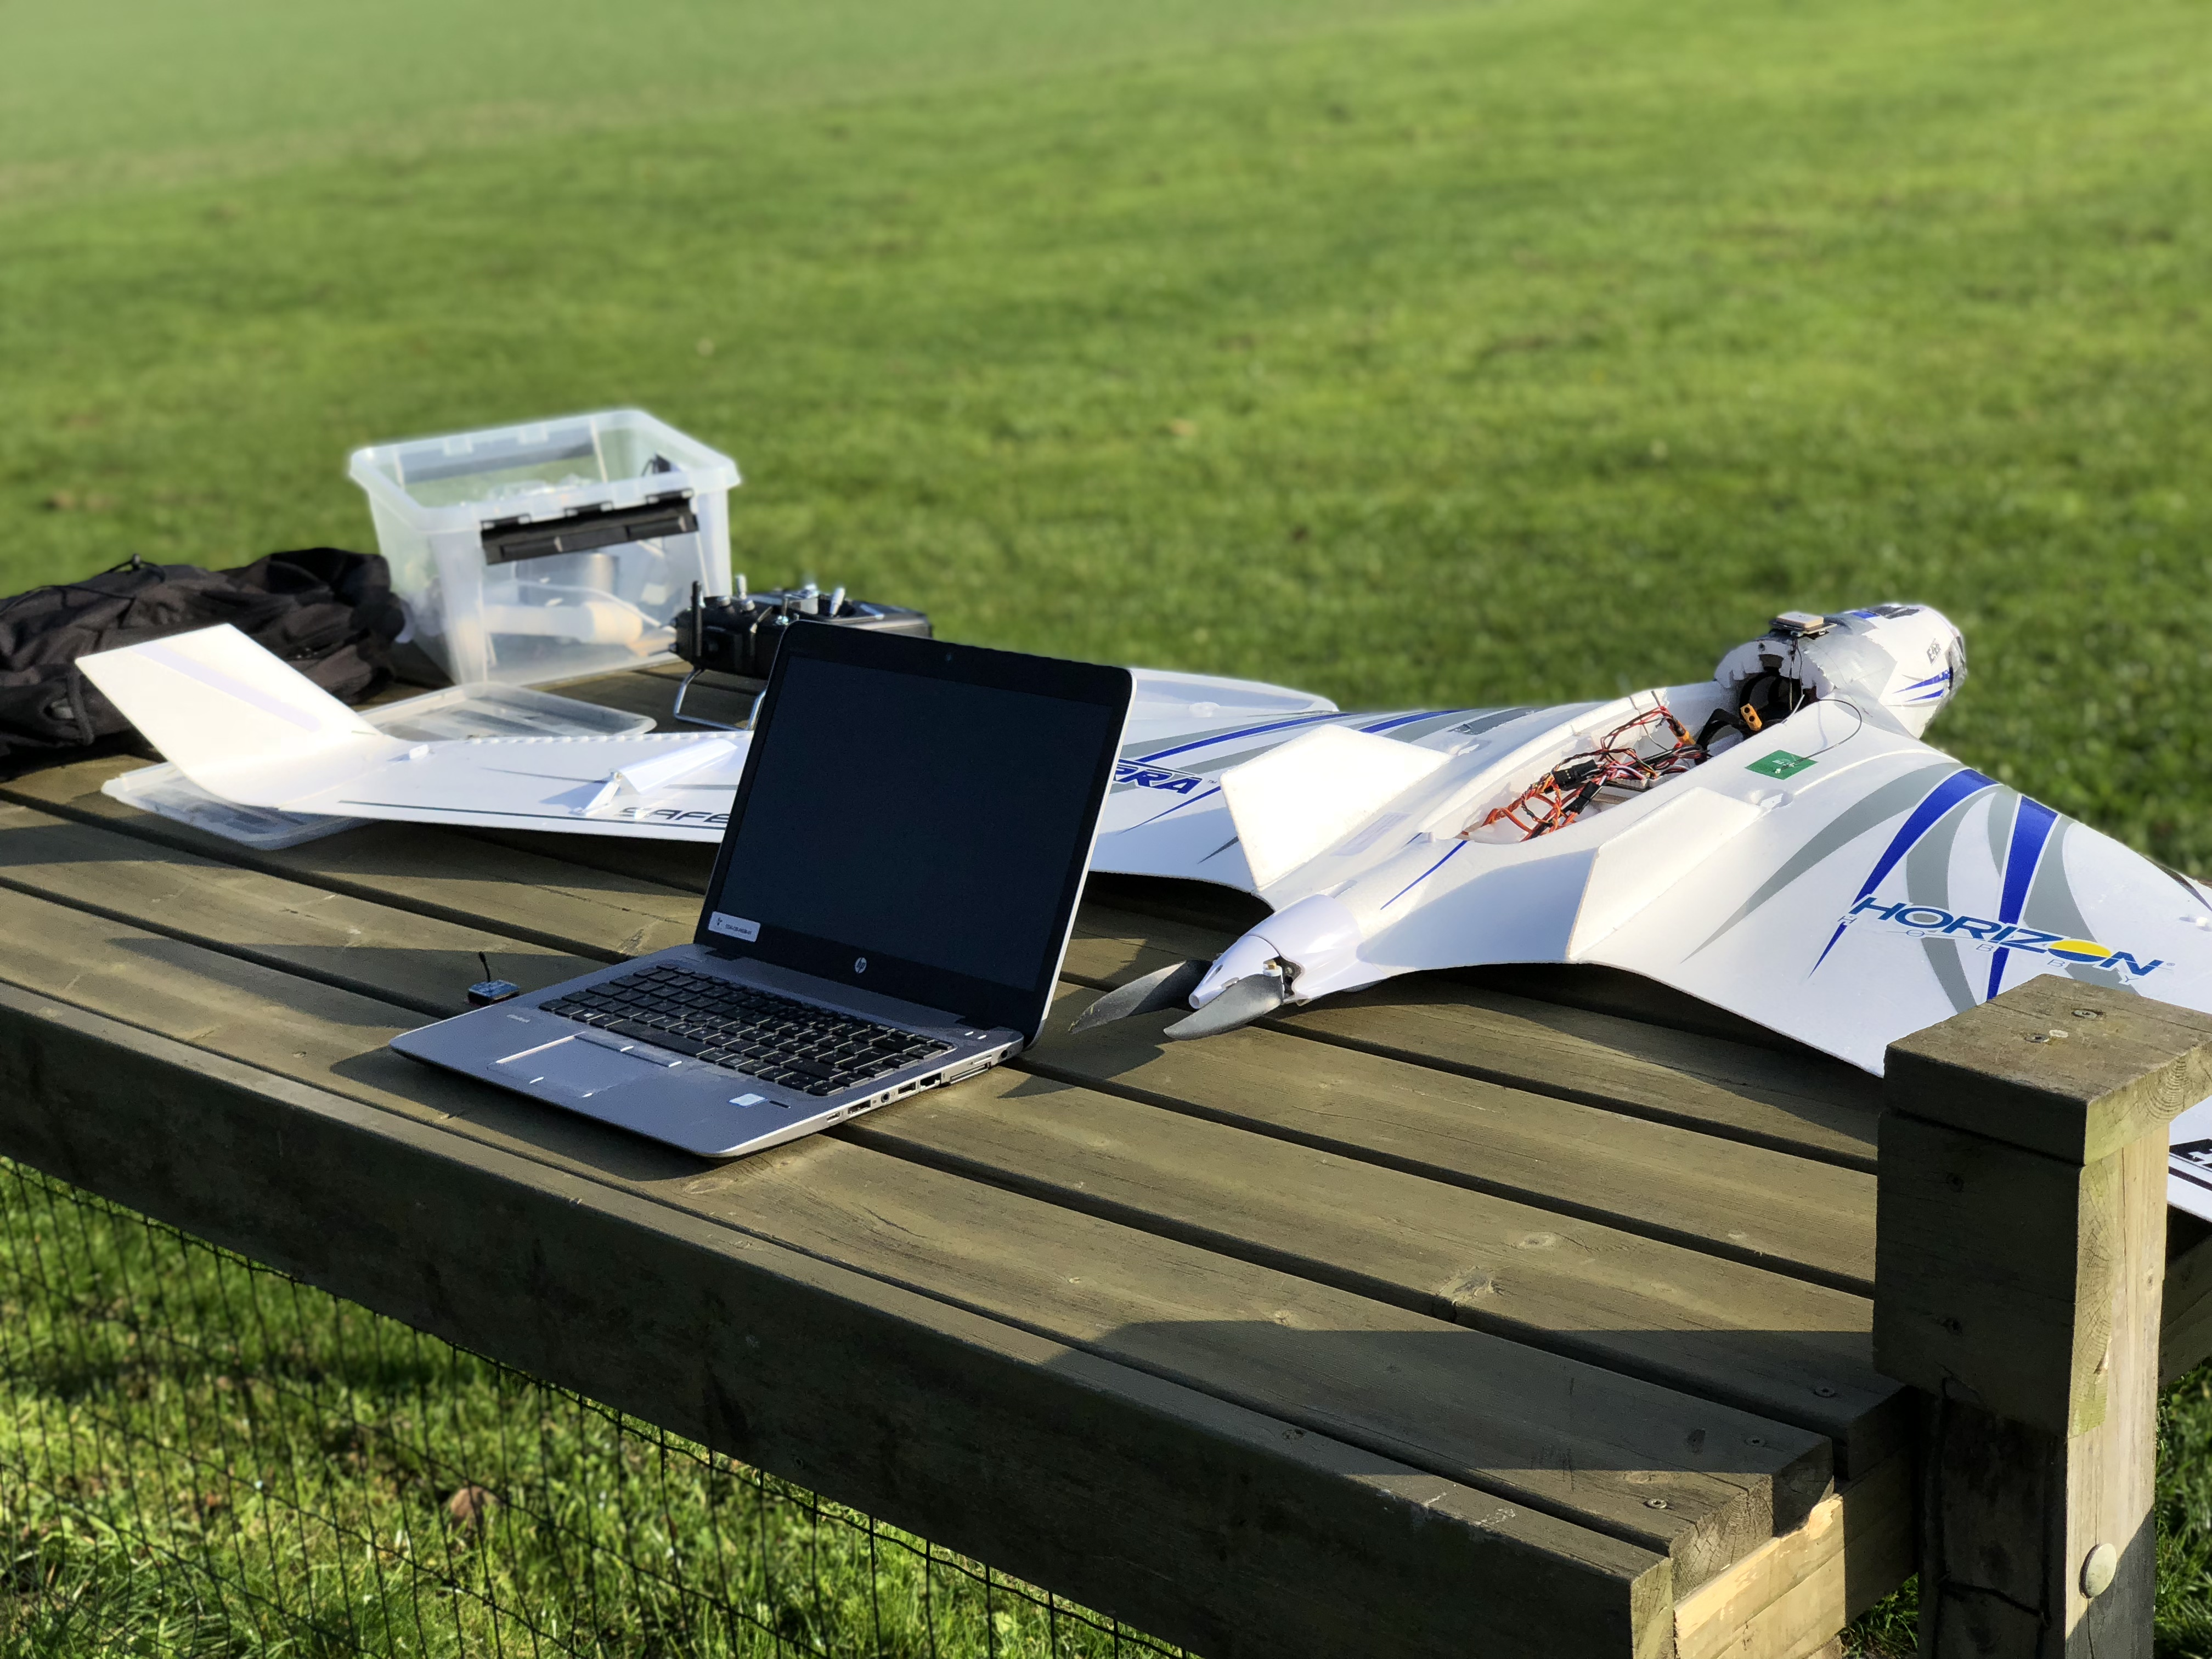
\includegraphics[width=.7\textwidth]{pictures/photo}
  \caption[Opterra fixed-wing drone]{Opterra fixed-wing drone employed as an aerial robotics platform for precision agriculture {\scriptsize(photo credit: Amit Ferencz Appel)}.}   
  \label{fig:opterra}
\end{figure}

We investigate different physical aerial robotics platforms in this work but we focus most on the Opterra fixed-wing drone\findex{Opterra fixed-wing drone}~\citep{opterra} adapted for precision agriculture. Precision agriculture\findex{precision agriculture} is often put into practice~\citep{hajjaj2014review} with ground mobile robots used for harvesting~\citep{qingchun2012study,dong2011development, de2011design, aljanobi2010setup, li2008analysis, edan2000robotic}, and \Gls{acr:uav}s for preventing damage and ensuring better crop quality~\citep{puri2017agriculture, daponte2019review}. The aerial robot is shown in \fref{fig:opterra}{Figure}.

In the remainder of the chapter and before we introduce the problem in \fref{sec:pb-form}{Section}, we briefly investigate the evolution of the field of aerial robotics in the next section. We then analyze the main aerial robots available today, and how they apply to dynamic energy planning in \fref{sec:aerial-robo-types}{Section}. We then provide some further motivation for our planning in \fref{sec:motivation}{Section} and the outline of the approach in \fref{sec:outline}{Section}. Finally, we provide the structure of the remaining chapters in \fref{sec:structure}{Section}.

This chapter connects to the remainder of this work as follows. Here we present some definitions and formalize the planning problem. We describe the derivation of a proper energy model to predict the future energy consumption of the planning problem in \fref{cp:model}{Chapter}. We estimate some coefficients of the model using robust estimation techniques in \fref{cp:est}{Chapter}. We implement an optimal configuration of the path and computations using data-driven control\findex{data-driven control} and other modern optimal control techniques in \fref{cp:opt}{Chapter}. This optimal configuration solves the planning problem from this chapter. We use such configuration for guidance and scheduling of the aerial robot in \fref{cp:gd}{Chapter}. The guidance moves physically the robot; the scheduling defines the granularity of the tasks being executed in flight. Moreover, we describe previous approaches to solve the dynamic planning problem in \fref{cp:soa}{Chapter}. 


%%%%%%%%%%%%%%%%%%%%%%%%%%%%%%%%%%%%%%%%%%%
\section{From UAVs to Modern Aerial Robots}

Modern aerial robots are a valuable tool in robotic research and aerospace. They are found with different names in the literature. These include unmanned aerial vehicles\findex{unmanned aerial vehicles} (\Gls{acr:uav}s)\footnote{The term unmanned is sometimes replaced by uninhabited}, unmanned aerial systems\findex{unmanned aerial systems} (\Gls{acr:uas}s), flying robots, or drones. Usually, we refer to drones, \Gls{acr:uav}s, and \Gls{acr:uas}s when these systems are semi-autonomous, operated from the ground. \Gls{acr:uas} often denotes the entire infrastructure of unmanned flight in the aerospace jargon. Aerial or flying robots, on the other hand, have advanced levels of autonomy~\citep{siciliano2016springer}. Nevertheless, all these systems have basic autonomous features such as position and altitude holding and leveling. The position holding is usually implemented using global navigation satellite system\findex{global navigation satellite system} (\Gls{acr:gnss}), altitude holding using a barometer\findex{barometer}, and leveling using inertial measurement unit\findex{inertial measurement unit} (\Gls{acr:imu}).

\begin{figure}[t]
  \centering
  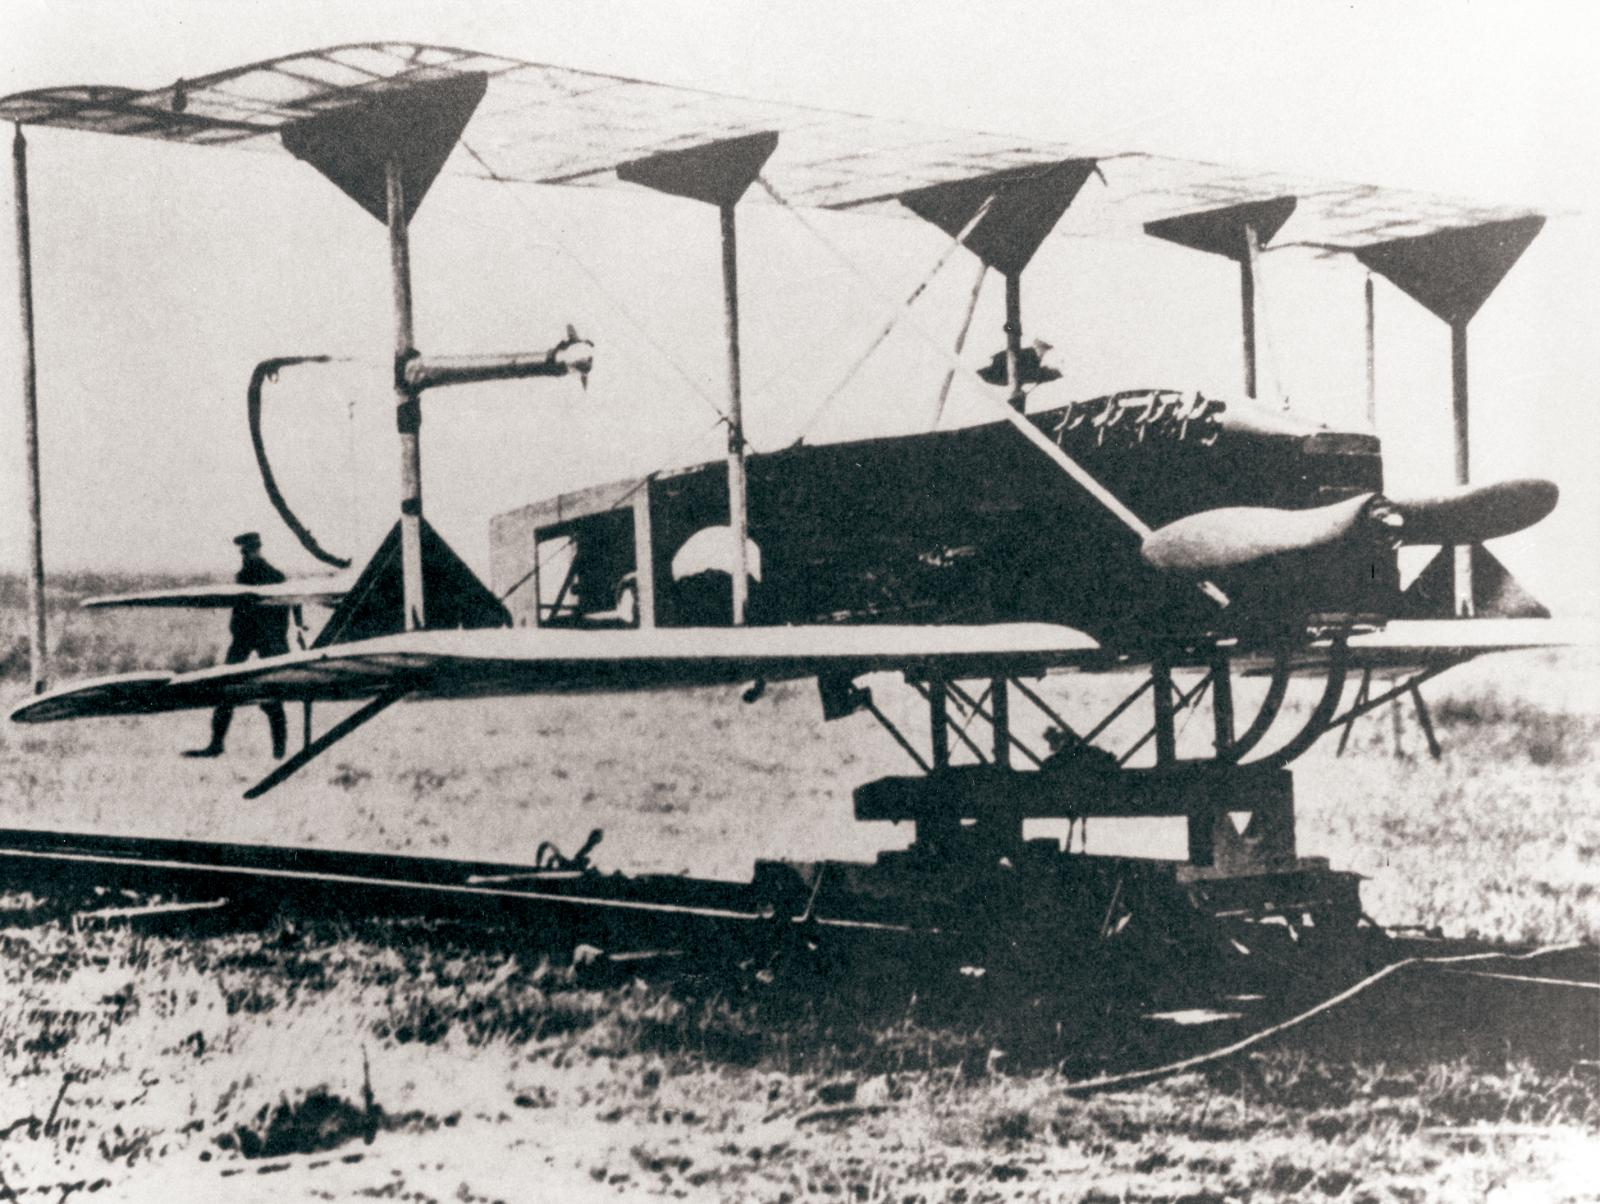
\includegraphics[width=.7\textwidth]{pictures/HA-NH-JA-19_1}
  \caption[Hewitt-Sperry Automatic Airplane, first unmanned flying machine]{The Hewitt-Sperry Automatic Airplane, also denominated ``flying bomb'', was developed in WWI and represents the first instance of a \Gls{acr:uav} {\scriptsize(photo credit: United States Naval Institute)}.}   
  \label{fig:hewitt-sperry}
\end{figure}

The origin of the field of aerial robotics, which deals with the design and development of aerial robots, dates back to the first guided missiles~\citep{siciliano2016springer}. Indeed unmanned (or uninhabited) flight has more than a century of developments~\citep{siciliano2016springer}. Hewitt-Sperry Automatic Airplane\findex{Hewitt-Sperry automatic airplane}, also denominated ``flying bomb'', developed in 1917 during World War I\findex{World War I} (WWI)~\citep{keane2013brief,valavanis2015handbook} is often referred to as the first unmanned flying machine. It is shown in \fref{fig:hewitt-sperry}{Figure}. The milestone has been reached just 14 years after the first heavier-than-air flight in history. The latter has been demonstrated on December 17, 1903, with the Wright Flyer I by Wilbur and Orville Wright\findex{Wright brother} (or the Wright brothers). The Hewitt-Sperry Automatic Airplane used a gyroscope\findex{gyroscope} similarly to modern aerial robots. The device, invented by Elmer Sperry~\citep{keane2013brief}, was mechanically connected to the control surfaces and successfully implemented a control feedback loop~\citep{siciliano2016springer}.

In the early days, these flying machines were labeled remotely piloted vehicles\findex{remotely piloted vehicles} (\Gls{acr:rpv}s)~\citep{anderson2005introduction}. Many instances from WWI on of the early \Gls{acr:uav}s were designed for military purposes. In the 1950s, United States used a remotely controlled vehicle, the Ryan Firebee\findex{Ryan Firebee}, for reconnaissance in Vietnam, and Israel was the first to use a \Gls{acr:rpv} in a combat situation~\citep{anderson2005introduction}. Other instances of these vehicles include the V-1 flying bomb~\findex{V-1 flying bomb} from 1944 (deployed by the unified armed forces of nazi Germany) and the Lockheed D-21~\findex{Lockheed D-21} from 1962 (deployed by the United States Air Force). Global positioning system\findex{global positioning system} (\Gls{acr:gps}) at the end of 1970 allowed the \Gls{acr:uav}s to be used in surveillance. These systems were later integrated with cameras and other sensors~\citep{siciliano2016springer}, in what are the modern aerial robots.

In recent years, the unmanned flight has been applied in many civilian applications~\citep{gonzalez2017unmanned}. Modern aerial robots are increasingly used in remote sensing\findex{remote sensing}~\citep{noor2018remote,tang2015drone,milas2018drones}, surveillance\findex{surveillance}~\citep{paucar2018use,burkle2009collaborating}, meteorology\findex{meteorology}~\citep{schuyler2019using}, search and rescue\findex{search and rescue}~\citep{pensieri2020drones,karaca2018potential,cui2015drones,seguin2018unmanned}, precision agriculture~\citep{daponte2019review,puri2017agriculture}, transportation, and payload delivery\findex{payload delivery}~\citep{kellermann2020drones}. The former four categories fall into the area of reconnaissance, surveillance, and target acquisition\findex{reconnaissance, surveillance, and target acquisition} (\Gls{acr:rsta}) and do not require advanced autonomy. Precision agriculture, transportation, and payload delivery are often realized using to a greater or lesser extent some advanced levels of computational intelligence~\citep{siciliano2016springer}. Modern aerial robots are designed to handle unexplored terrain with little interaction as opposed to the past \Gls{acr:uav}s operated mainly by a human operator~\citep{siciliano2016springer}. Instances of modern aerial robots are expected to autonomously adapt and possibly interact in a broad variety of environmental conditions. 

\begin{figure}[t]
  \centering
  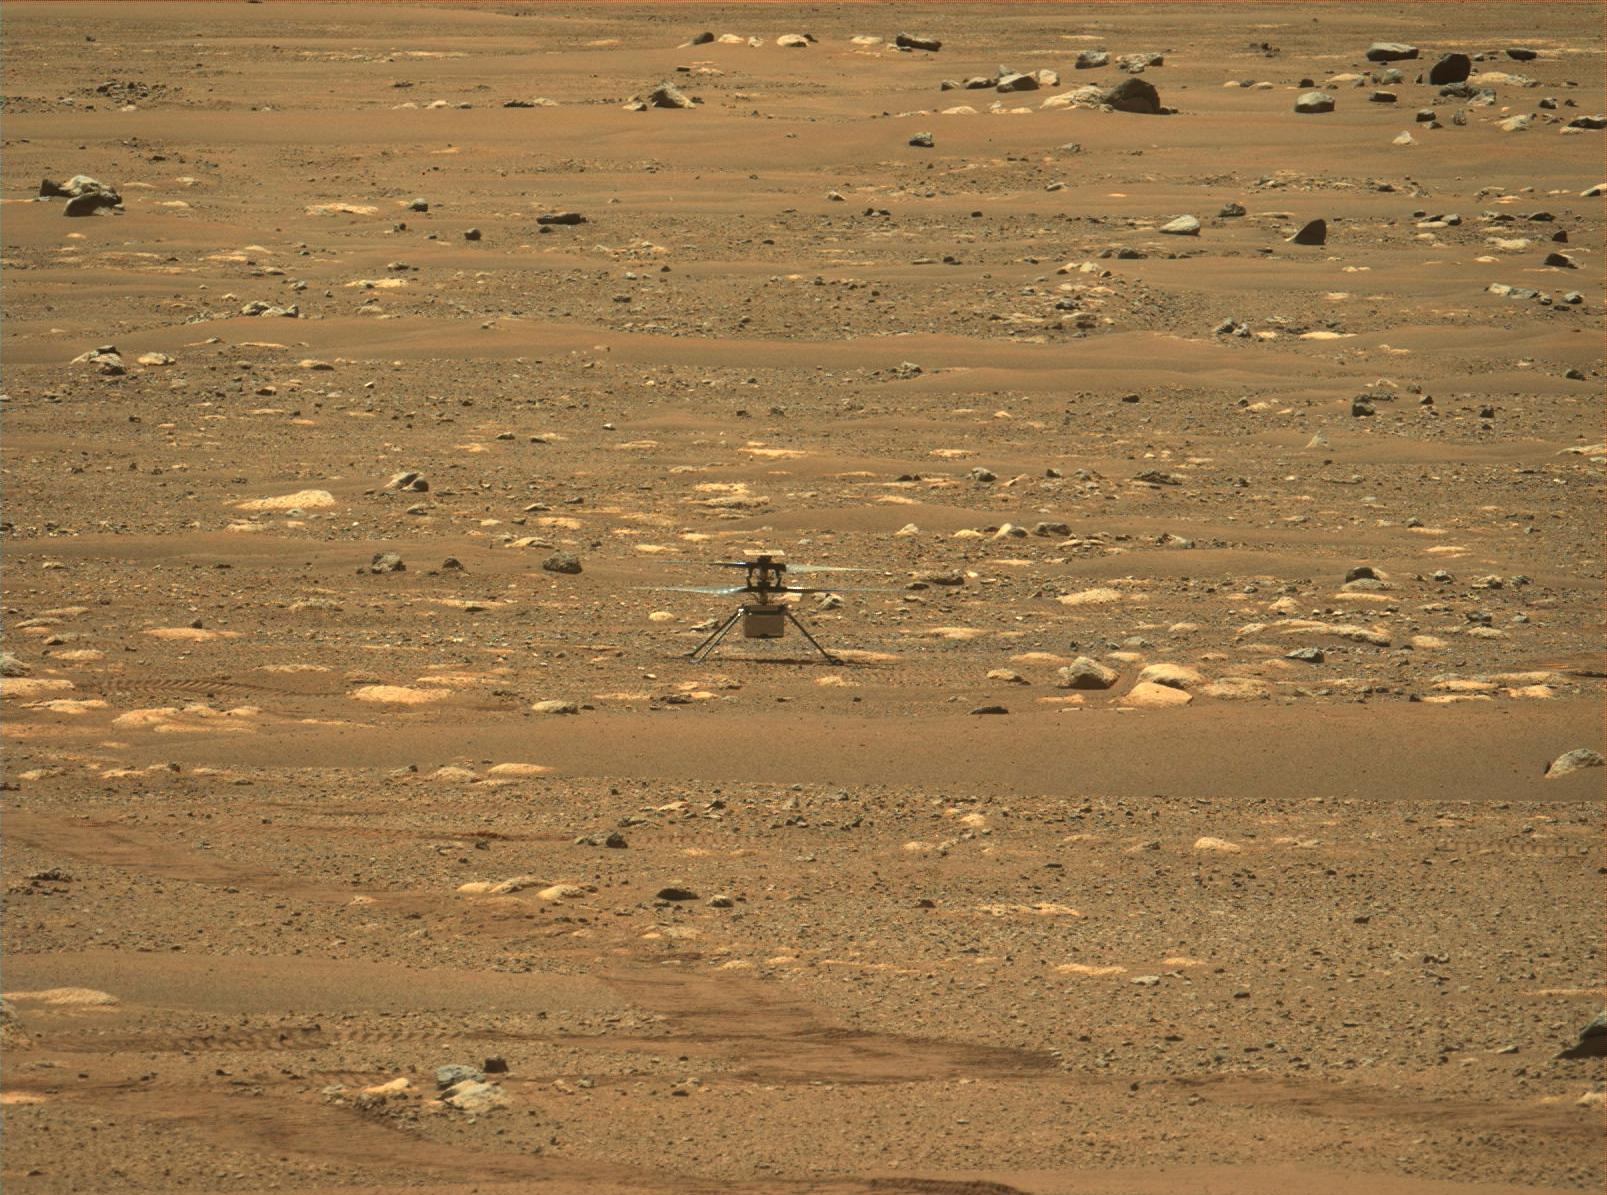
\includegraphics[width=.7\textwidth]{pictures/jpegPIA24550}
  \caption[NASA's Ingenuity Mars Helicopter]{NASA's Ingenuity Mars Helicopter. A rotary-wing coax aerial robot that achieved the first powered, controlled flight on another planet on April 19, 2021. The project is solely a demonstration of technology {\scriptsize(photo credit: NASA Jet Propulsion Laboratory)}.}   
  \label{fig:ingenuity}
\end{figure}

In summary, aerial robots have a relatively recent past. Some initial experiments of unmanned flights were performed shortly after the first heavier-than-air manned, powered flight. These initial experiments were mostly developed for military purposes, whereas modern aerial robots are used in a broad range of civil applications. Aerial robots are expected to grow significantly in numerous areas of robotics research ranging from agriculture to planetary exploration. For the latter, \fref{fig:ingenuity}{Figure} shows NASA's Ingenuity Mars Helicopter. A small coaxial aerial robot that performed the first powered, controlled flight on another planet on April 19, 2021. Aerial robots for planetary exploration are to be further deployed in future explorations endeavors, for instance, to study Saturn's moon Titan~\citep{voosen2019nasa}.

Finally, we conclude this section with a quote from~\citep{anderson2005introduction}: ``the Wright brothers worked so hard to put humans in the air in flying machines, a hundred years later some [...] are working hard to take them out of flying machines''.


%%%%%%%%%%%%%%%%%%%%%%%%%%%%%%%%%%%%%%%%%
\section{Common Classes of Aerial Robots}
\label{sec:aerial-robo-types}

Numerous different types of aerial robots have emerged ever since their first introduction. We briefly investigate the most studied classes in the robotics literature and relate them to the dynamic energy planning that we focus on in this work. The two most generic classes are heavier-than-air and lighter-than-air aerial robots. Heavier-than-air aerial robots\findex{heavier-than-air aerial robots} are divided into fixed- and rotary-wings~\citep{siciliano2016springer}, and some recent developments in bio-inspired robotics study flapping-wings~\citep{floreano2015science}\findex{flapping-wings}. 

Rotary-wing aerial robots\findex{rotary-wings} are highly maneuverable and can perform stationary vertical flight (commonly referred to as hovering\findex{hovering})~\citep{siciliano2016springer}. These systems can be classified into further categories, which include multirotors\findex{multirotors} (such as quadrotors\findex{quadrotors} or quadcopters\findex{quadcopters}, hexacopters\findex{hexacopters}, and octocopters\findex{octocopters}), conventional helicopters\findex{helicopters} (these have one main and one tail rotor), and a coax\findex{coax} (these have counter-rotating coaxial rotors)~\citep{corke2017robotics}. Some examples of quadrotors are DJI Mavic Mini in \sref{lab:mavic}, and DJI Phantom 4 in \sref{lab:phantom} in \fref{fig:plot10}{Figure}. In the same figure, DJI Agras T16 in \sref{lab:agras}, and DJI Matrice 600 in \sref{lab:matrice} are hexacopters.

Fixed-wing aerial robots\findex{fixed-wings} have wings to provide the lift, some control surfaces for maneuvering, and a propeller for forwarding thrust; a shared principle with a common passenger aircraft~\citep{corke2017robotics}. An example constitutes the Opterra adapted for precision agriculture in \fref{fig:opterra}{Figure}, Cumulus in \sref{lab:cumulus}, Ebee in \sref{lab:ebee}, and Penguin BE in \sref{lab:penguin}~\citep{haugen2016monitoring} in \fref{fig:plot10}{Figure}. Examples of flapping-wings are Delfly II in \sref{lab:delfly}~\citep{percin2012flow}, and Nano-Hummingbird in \sref{lab:nano} in \fref{fig:plot10}{Figure}. We discuss in detail heavier-than-air aerial robots in this work, as they are a common platform for robotics research. We focus on the dynamic forces which govern the flight of rotary- and fixed-wings aerial robots in \fref{cp:gd}{Chapter}.

Common instances of lighter-than-air aerial robots\findex{lighter-than-air aerial robots} are blimps\findex{blimps} (or non-rigid airships). They usually rely on a gas--such as helium enclosed in a protected envelope~\citep{burri2013design}--to generate the lifting force~\citep{fui2017recent}. An omnidirectional spherical blimp is shown in \fref{fig:skye-blimp}{Figure}. Blimps are similar to balloons but provide basic maneuverability, whereas, in a balloon, only the altitude can be controlled~\citep{colombatti2011lighter}.

\begin{figure}[t]
  \centering
  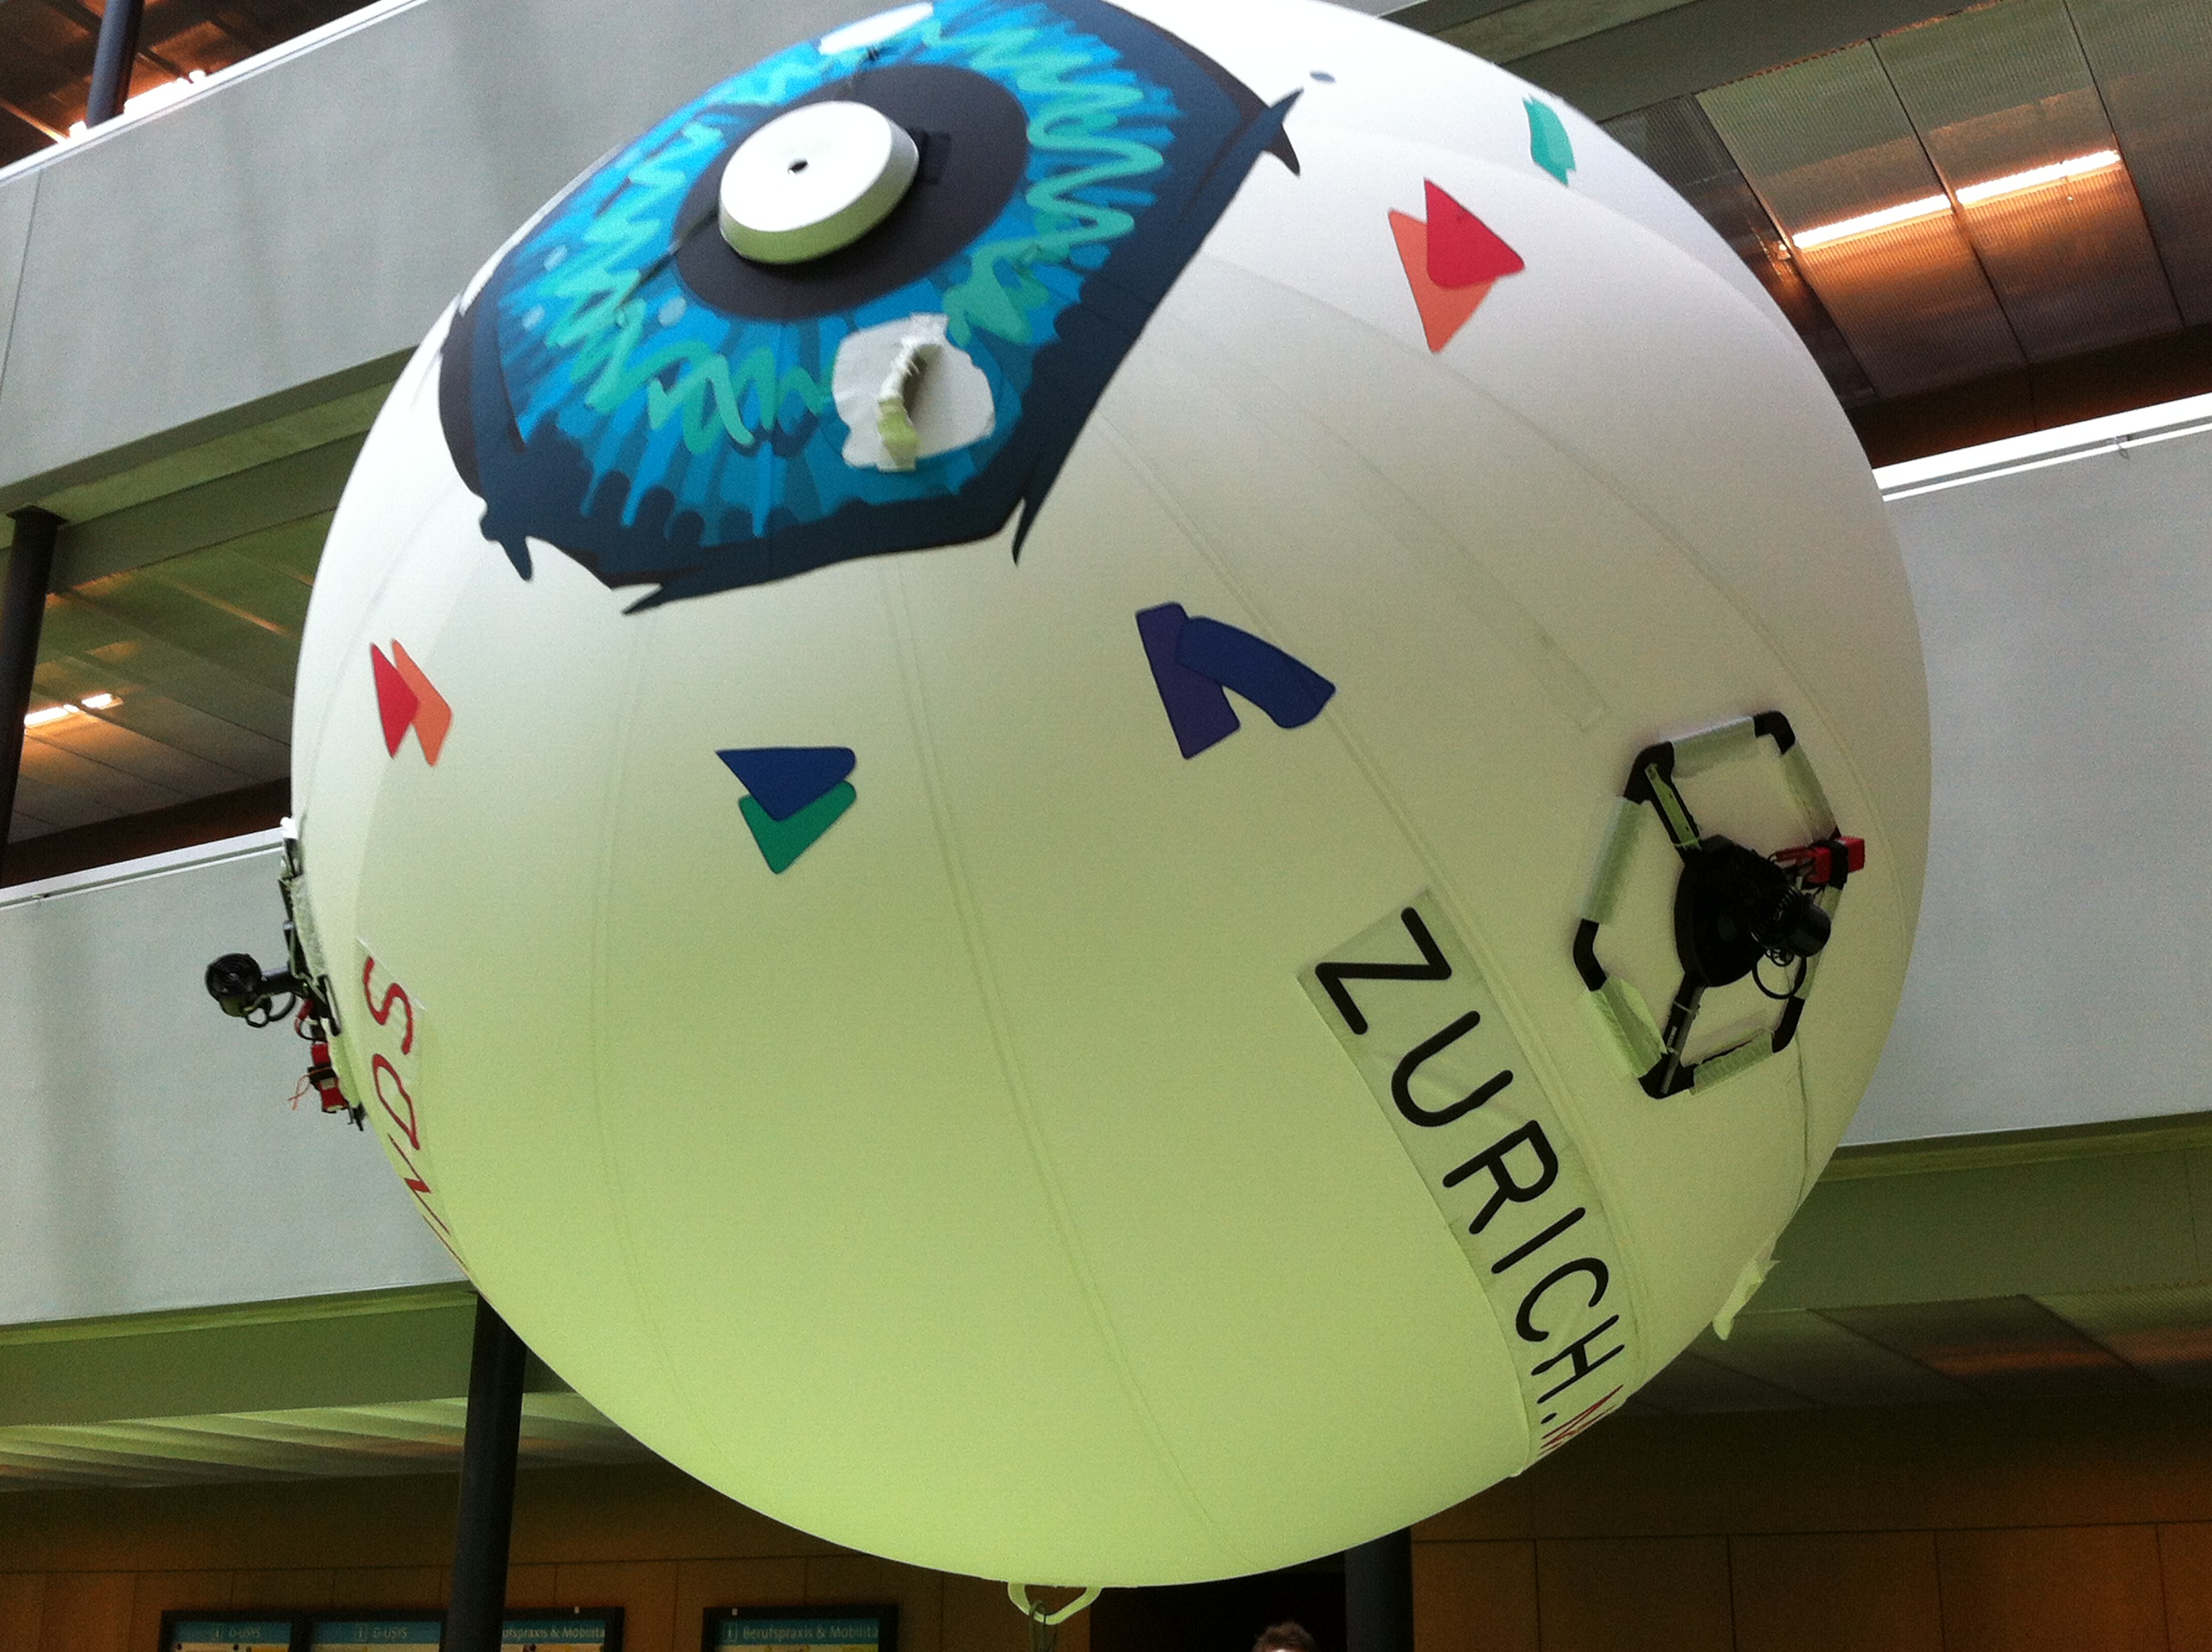
\includegraphics[width=.7\textwidth]{pictures/IMG_2612}
  \caption[Skye, an omnidirectional spherical blimp]{Skye, an omnidirectional spherical blimp developed by ETH Z\"urich for entertainment purposes. It has a camera system and combines the energy-efficient flight of a blimp with the characteristics of a quadrotor {\scriptsize(photo credit: ETH Z\"urich)}.}   
  \label{fig:skye-blimp}
\end{figure}

Some other classifications found in aerial robotics literature trade size and maneuverability and include classes as micro aerial vehicles (MAVs)\findex{micro aerial vehicles} or vertical take-off and landing (VTOLs)\findex{vertical take-off and landing} aerial robots. The former are aerial robots with all dimensions lower than 15 cm. The latter are aerial robots flying in a fixed-wing configuration except if taking-off and landing where they use thrust from rotors rather than lift from wings. 

Among the classes in this section, rotary-wings are the most maneuverable and lighter-than-air aerial robots are the least. These, however, have the highest flight time followed by fixed-wing aerial robots. Flapping-wings and mixed configurations, such as VTOLs, fall into the intersection of rotary and fixed-wings for what concerns maneuverability and flight time~\citep{siciliano2016springer}. The energy requirements are critical for all aerial robots, but the difference of motion and computations energy (\Gls{acr:mace}) varies greatly. The energy--inversely proportional to flight time--is highest in rotary-wings and lowest in lighten-than-air aerial robots as shown later in \fref{fig:plot10}{Figure}. The dynamic energy planning approach thus relies on both power-saving task scheduling and energy-efficient path planning for the fixed-wings robots while relying almost exclusively on energy-efficient path planning for rotary-wing aerial robots. In the former \Gls{acr:mace} is close to zero, in the latter is usually high except in energy optimized designs such as some rotary-wing MAVs. Hypothetically, in lighter-than-air aerial robots, \Gls{acr:mace} might be negative; the energy planning approach would rely heavily on power-saving task scheduling.


%%%%%%%%%%%%%%%%%%%%
\section{Motivation}
\label{sec:motivation}

\begin{figure}[t]
  \centering
  \footnotesize\fontfamily{phv}\selectfont
  
\definecolor{cF5F5F5}{RGB}{245,245,245}
\definecolor{cE4E4E4}{RGB}{218,218,218}
\definecolor{cFFFFFF}{RGB}{255,255,255}


\def \globalscale {1.000000}
\begin{tikzpicture}[y=0.80pt, x=0.80pt, yscale=-\globalscale, xscale=\globalscale, inner sep=0pt, outer sep=0pt]
\path[fill=cF5F5F5,line join=round,line width=0.160pt] (49.4778,304.7930) .. controls (49.4778,304.7930) and (59.8838,312.4890) .. (61.2031,312.8170) .. controls (70.4387,315.1130) and (100.8800,325.1290) .. (113.9110,320.3850) .. controls (113.9110,320.3850) and (128.5000,319.7570) .. (145.0340,312.7870) .. controls (161.5680,305.8160) and (145.5200,259.4940) .. (145.5200,259.4940) .. controls (145.5200,259.4940) and (142.1620,253.0560) .. (134.1470,241.3320) .. controls (117.8560,217.5040) and (93.7304,210.8650) .. (93.7304,210.8650) .. controls (93.7304,210.8650) and (63.8068,187.8810) .. (25.8309,187.8090) .. controls (25.8308,187.8090) and (-22.5721,198.7600) .. (27.1148,283.8080) -- (49.4778,304.7930) -- cycle;



\path[fill=cE4E4E4,line join=round,line width=0.160pt] (127.5850,194.5280) .. controls (127.5850,194.5280) and (134.1470,175.0990) .. (158.4610,168.6670) .. controls (182.7760,162.2360) and (231.4050,165.3730) .. (280.0340,151.6470) .. controls (328.6630,137.9210) and (369.0490,168.6670) .. (369.0490,168.6670) .. controls (369.0490,168.6670) and (406.9790,216.5900) .. (336.4670,259.4940) .. controls (265.9550,302.3970) and (189.5610,259.9450) .. (182.7760,254.0000) .. controls (175.9910,248.0540) and (138.0740,250.1440) .. (129.7840,235.1790) .. controls (121.4930,220.2140) and (121.4250,207.4960) .. (127.5850,194.5280) -- cycle;



\path[fill=foo,line join=round,line width=0.160pt] (169.3250,153.3220) .. controls (169.3250,153.3220) and (214.3850,166.4820) .. (231.4050,160.2860) .. controls (231.4050,160.2860) and (248.7700,157.3510) .. (265.3040,150.3810) .. controls (281.8380,143.4110) and (280.0340,102.4370) .. (280.0340,102.4370) .. controls (280.0340,102.4370) and (278.7420,90.4098) .. (280.0340,76.2665) .. controls (282.4490,49.8338) and (244.5430,30.6534) .. (244.5430,30.6534) .. controls (244.5430,30.6534) and (236.2680,14.3982) .. (134.1470,38.7128) .. controls (134.1470,38.7128) and (106.5590,38.7128) .. (123.0930,135.9710) .. controls (123.0930,135.9710) and (144.3610,149.3270) .. (149.3680,151.1110) .. controls (154.3750,152.8940) and (169.0830,153.1350) .. (169.3250,153.3220) -- cycle;

\path[cm={{1.0,0.0,0.0,1.0,(0,0)}}] (0.0000,0.0000) node[below right] () {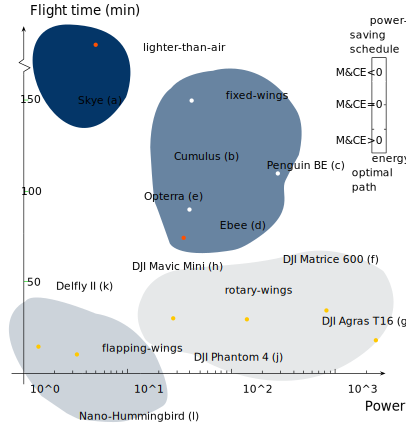
\includegraphics[width=4.25in]{figures/source/plot10}};

\path[fill=foo,line join=round,line width=0.160pt] (319.5490,240.6600) .. controls (320.7430,240.6600) and (321.7110,241.6280) .. (321.7110,242.8220) .. controls (321.7110,244.0160) and (320.7430,244.9840) .. (319.5490,244.9840) .. controls (318.3550,244.9840) and (317.3870,244.0160) .. (317.3870,242.8220) .. controls (317.3870,241.6280) and (318.3550,240.6600) .. (319.5490,240.6600) -- cycle;



\path[fill=foo,line join=round,line width=0.160pt] (269.0760,214.8400) .. controls (270.2700,214.8400) and (271.2380,215.8080) .. (271.2380,217.0020) .. controls (271.2380,218.1960) and (270.2700,219.1640) .. (269.0760,219.1640) .. controls (267.8820,219.1640) and (266.9140,218.1960) .. (266.9140,217.0020) .. controls (266.9140,215.8080) and (267.8820,214.8400) .. (269.0760,214.8400) -- cycle;



\path[fill=foo,line join=round,line width=0.160pt] (208.4930,224.7000) .. controls (209.6870,224.7000) and (210.6550,225.6680) .. (210.6550,226.8620) .. controls (210.6550,228.0560) and (209.6870,229.0240) .. (208.4930,229.0240) .. controls (207.2990,229.0240) and (206.3310,228.0560) .. (206.3310,226.8620) .. controls (206.3310,225.6680) and (207.2990,224.7000) .. (208.4930,224.7000) -- cycle;



\path[fill=foo,line join=round,line width=0.160pt] (201.7350,224.7000) .. controls (202.9290,224.7000) and (203.8970,225.6680) .. (203.8970,226.8620) .. controls (203.8970,228.0560) and (202.9290,229.0240) .. (201.7350,229.0240) .. controls (200.5410,229.0240) and (199.5730,228.0560) .. (199.5730,226.8620) .. controls (199.5730,225.6680) and (200.5410,224.7000) .. (201.7350,224.7000) -- cycle;



\path[fill=cFFFFFF,line join=round,line width=0.160pt] (231.4380,85.7318) .. controls (232.6320,85.7318) and (233.6000,86.6998) .. (233.6000,87.8938) .. controls (233.6000,89.0879) and (232.6320,90.0560) .. (231.4380,90.0560) .. controls (230.2440,90.0560) and (229.2760,89.0879) .. (229.2760,87.8938) .. controls (229.2760,86.6998) and (230.2440,85.7318) .. (231.4380,85.7318) -- cycle;



\path[fill=cFFFFFF,line join=round,line width=0.160pt] (196.7440,73.3687) .. controls (197.9380,73.3687) and (198.9060,74.3367) .. (198.9060,75.5307) .. controls (198.9060,76.7248) and (197.9380,77.6928) .. (196.7440,77.6928) .. controls (195.5500,77.6928) and (194.5820,76.7248) .. (194.5820,75.5307) .. controls (194.5820,74.3367) and (195.5500,73.3687) .. (196.7440,73.3687) -- cycle;



\path[fill=cFFFFFF,line join=round,line width=0.160pt] (195.2150,96.1679) .. controls (196.4090,96.1679) and (197.3770,97.1359) .. (197.3770,98.3300) .. controls (197.3770,99.5240) and (196.4090,100.4920) .. (195.2150,100.4920) .. controls (194.0210,100.4920) and (193.0530,99.5240) .. (193.0530,98.3300) .. controls (193.0530,97.1359) and (194.0210,96.1679) .. (195.2150,96.1679) -- cycle;



\path[fill=cFFFFFF,line join=round,line width=0.160pt] (192.0210,91.8550) .. controls (193.2150,91.8550) and (194.1830,92.8230) .. (194.1830,94.0171) .. controls (194.1830,95.2111) and (193.2150,96.1791) .. (192.0210,96.1791) .. controls (190.8270,96.1791) and (189.8590,95.2111) .. (189.8590,94.0171) .. controls (189.8590,92.8230) and (190.8270,91.8550) .. (192.0210,91.8550) -- cycle;



\path[fill=foo,line join=round,line width=0.160pt] (77.3763,248.8450) .. controls (78.5704,248.8450) and (79.5384,249.8130) .. (79.5384,251.0070) .. controls (79.5384,252.2010) and (78.5704,253.1690) .. (77.3763,253.1690) .. controls (76.1823,253.1690) and (75.2143,252.2010) .. (75.2143,251.0070) .. controls (75.2143,249.8130) and (76.1823,248.8450) .. (77.3763,248.8450) -- cycle;



\path[fill=foo,line join=round,line width=0.160pt] (72.8985,245.0460) .. controls (74.0925,245.0460) and (75.0605,246.0140) .. (75.0605,247.2080) .. controls (75.0605,248.4020) and (74.0925,249.3700) .. (72.8985,249.3700) .. controls (71.7044,249.3700) and (70.7364,248.4020) .. (70.7364,247.2080) .. controls (70.7364,246.0140) and (71.7044,245.0460) .. (72.8985,245.0460) -- cycle;



\path[fill=foo,line join=round,line width=0.160pt] (19.1786,12.9659) .. controls (20.3727,12.9659) and (21.3407,13.9339) .. (21.3407,15.1280) .. controls (21.3407,16.3221) and (20.3727,17.2901) .. (19.1786,17.2901) .. controls (17.9845,17.2901) and (17.0165,16.3221) .. (17.0165,15.1280) .. controls (17.0165,13.9339) and (17.9845,12.9659) .. (19.1786,12.9659) -- cycle;



\path[fill=black,line join=round,line width=0.160pt] (320.5760,257.0980) -- (322.5520,259.3950) -- (320.5300,261.4530) -- (326.3250,259.3400) -- (320.5760,257.0980) -- cycle;



\path[fill=black,line join=round,line width=0.160pt] (180.7460,21.4106) -- (183.0180,19.4057) -- (185.1020,21.4014) -- (182.9160,15.6335) -- (180.7460,21.4106) -- cycle;



\path[draw=black,line join=round,line width=0.512pt] (41.4555,259.3320) -- (322.6080,259.3320);



\path[draw=black,line join=round,line width=0.512pt] (183.0230,266.9540) -- (183.0230,156.7750);



\path[draw=cFFFFFF,line join=round,line width=0.512pt] (183.0230,156.7750) -- (183.0230,28.8031);



\path[draw=black,line join=round,line width=0.512pt] (183.0230,28.8031) -- (183.0230,18.3373);



  \path[cm={{1.0,0.0,0.0,1.0,(240.0,39.0)}}] (0.0000,0.0000) node[above right] () {{\color{white}fix}ed-wings};



  \path[cm={{1.0,0.0,0.0,1.0,(138.0,11.0)}}] (0.0000,0.0000) node[above right] () {flight time};



  \path[cm={{1.0,0.0,0.0,1.0,(128.0,240.0)}}] (0.0000,0.0000) node[above right] () {\scriptsize DJI Mavic Mini  \textlabel{(h)}{lab:mavic}};



  \path[cm={{1.0,0.0,0.0,1.0,(303.0,239.0)}}] (0.0000,0.0000) node[above right] () {\scriptsize DJI Agras T16  \textlabel{(g)}{lab:agras}};



  \path[cm={{1.0,0.0,0.0,1.0,(223.0,213.0)}}] (0.0000,0.0000) node[above right] () {\scriptsize DJI Matrice 600  \textlabel{(f)}{lab:matrice}};



  \path[cm={{1.0,0.0,0.0,1.0,(209.0,276.0)}}] (0.0000,0.0000) node[above right] () {\scriptsize DJI Phantom 4  \textlabel{(j)}{lab:phantom}};



  \path[cm={{1.0,0.0,0.0,1.0,(138.0,86.0)}}] (0.0000,0.0000) node[above right] () {\scriptsize\color{white} Cumulus \textlabel{(b)}{lab:cumulus}};



  \path[cm={{1.0,0.0,0.0,1.0,(208.0,150.0)}}] (0.0000,0.0000) node[above right] () {\scriptsize\color{white} Opterra \textlabel{(e)}{lab:opterra}};



  \path[cm={{1.0,0.0,0.0,1.0,(143.0,144.0)}}] (0.0000,0.0000) node[above right] () {\scriptsize\color{white} Ebee \textlabel{(d)}{lab:ebee}};



  \path[cm={{1.0,0.0,0.0,1.0,(212.0,83.0)}}] (0.0000,0.0000) node[above right] () {\scriptsize\color{white} Penguin BE  \textlabel{(c)}{lab:penguin}};



  \path[cm={{1.0,0.0,0.0,1.0,(66.0,311.0)}}] (0.0000,0.0000) node[above right] () {\scriptsize Nano-Hummingbird  \textlabel{(l)}{lab:nano}};



  \path[cm={{1.0,0.0,0.0,1.0,(19.0,257.0)}}] (0.0000,0.0000) node[above right] () {\scriptsize Delfly II  \textlabel{(k)}{lab:delfly}};



  \path[cm={{1.0,0.0,0.0,1.0,(35.0,71.0)}}] (0.0000,0.0000) node[above right] () {\scriptsize Skye \textlabel{(a)}{lab:skye}};



  \path[cm={{1.0,0.0,0.0,1.0,(302.0,157.0)}}] (0.0000,0.0000) node[above right] () {rotary-wings};



  \path[cm={{1.0,0.0,0.0,1.0,(321.0,277.0)}}] (0.0000,0.0000) node[above right] () {M\&CE};



  \path[cm={{1.0,0.0,0.0,1.0,(3.0,287.0)}}] (0.0000,0.0000) node[above right] () {flapping-wings};




\end{tikzpicture}


  \caption[Different aerial robots in relation to the M\&CE and flight time]{Different aerial robots in relation to the M\&CE and flight time. Heavier-than-air aerial robots \sref{lab:cumulus}{}--\sref{lab:nano}{} include flapping-wings \sref{lab:delfly}{},~\sref{lab:nano}{} and have a negative M\&CE (computations scheduling is to be accounted for most in planning), whereas rotary-wings have a positive M\&CE \sref{lab:matrice}{},~\sref{lab:agras}{} (path planning is to be accounted for most in dynamic planning). Some smaller rotary-wings have a M\&CE closer to zero \sref{lab:mavic}{},~\sref{lab:phantom}{}. In general, rotary-wings have a short flight time. Fixed-wings \sref{lab:cumulus}{}--\sref{lab:opterra}{} have a considerably longer flight time and M\&CE close to zero (computations scheduling and path planning have both to be accounted for in dynamic planning). Lighter-than-air aerial robots \sref{lab:skye}{} have hypothetically a relatively long flight time and lower than zero M\&CE {\scriptsize(photos credit: \srefscriptsize{lab:cumulus} to Sky-Watch, \srefscriptsize{lab:matrice} to Rise Above, \srefscriptsize{lab:agras} to Aeromotus, \srefscriptsize{lab:mavic} to Digital Photography Review, \srefscriptsize{lab:phantom} to ePHOTOzine, and \srefscriptsize{lab:nano} to DARPA)}.}
  \label{fig:plot10}
\end{figure}

Many applications that involve aerial robots have strict battery constraints. Although this is a common problem to most mobile robots, aerial robots are of particular concern. The autonomy of these systems is affected by the availability of the power source. In this section, we provide a brief motivation for dynamic energy planning of these systems. A typical example of an aerial robotics scenario is a robot following a path and performing some onboard computations. For instance, the robot might detect ground patterns and notify other ground-based actors with little human interaction in precision agriculture or another application. Aerial robots in this situation often carry some heterogeneous computing hardware\findex{heterogeneous computing hardware} which powers autonomous capabilities in these use cases and a microcontroller. Energy requirements of such computing hardware are a further complication in these scenarios. Computing hardware is involved in the planning and additionally often runs computer vision or other complex algorithms, whereas microcontroller\findex{microcontroller} runs motion primitives by directly interfacing actuators (such as servos\findex{servo} for the control surfaces\findex{control surface}) and motors\findex{motor}. It is thus advantageous to schedule the computations on the computing hardware and simultaneously to plan the path. 

\subsection{Path planning and computations scheduling}

It is uncommon to find a ready-to-use solution for both planning the path and scheduling the computations of these systems in an energy-aware fashion (we discuss in detail the state-of-the-art in this regard in \fref{cp:soa}{Chapter}). Planning the two aspects simultaneously would pose an advantage in terms of autonomy by, e.g., optimizing the path and computations in the function of the battery state of charge (\Gls{acr:soc}). 

For certain classes of aerial robots with \Gls{acr:mace} close or lower than zero, the autonomy can directly influence the battery state. For these classes, it is desirable to reschedule the computations energy-wise in-flight during a motion energy-demanding phase. For instance, a fixed-wing aerial robot might be flying headwinds (with the wind vector parallel and opposite to the direction of motion) and utilizing more energy than planned. It would be of advantage to reschedule the tasks accordingly to save energy needed for motion. During the same flight, the wind direction might suddenly change. The fixed-wing craft, now flying tailwinds, requires less motion energy. It could then potentially increase the level of computations by rescheduling the tasks. Later in the flight, the battery might be subject to sudden drops (due to e.g., temperature changes) requiring replanning again by, e.g., shortening the path. It is clear that planning the path and scheduling the computations simultaneously in all these cases is the most desirable course of action.

In \fref{fig:plot10}{Figure} we show the \Gls{acr:mace} against the flight time of different aerial robots. We observe that fixed-wings are the aerial robots that would advantage most from simultaneous path planning and computations scheduling. They have a \Gls{acr:mace} close to zero and a relatively long flight time. Although some rotary-wings have \Gls{acr:mace} also close to zero, their flight time is generally relatively short. Flapping-wing and lighter-than-air aerial robots require considerably less energy for the motion, and have a negative \Gls{acr:mace}.

\subsection{Objective}

\begin{figure}[t]
  \centering
  
\def \globalscale {1.000000}
\begin{tikzpicture}[y=0.80pt, x=0.80pt, yscale=-.7*\globalscale, xscale=.7*\globalscale, inner sep=0pt, outer sep=0pt]

\path[cm={{1.0,0.0,0.0,1.0,(0,0)}}] (0.0000,0.0000) node[below right] () {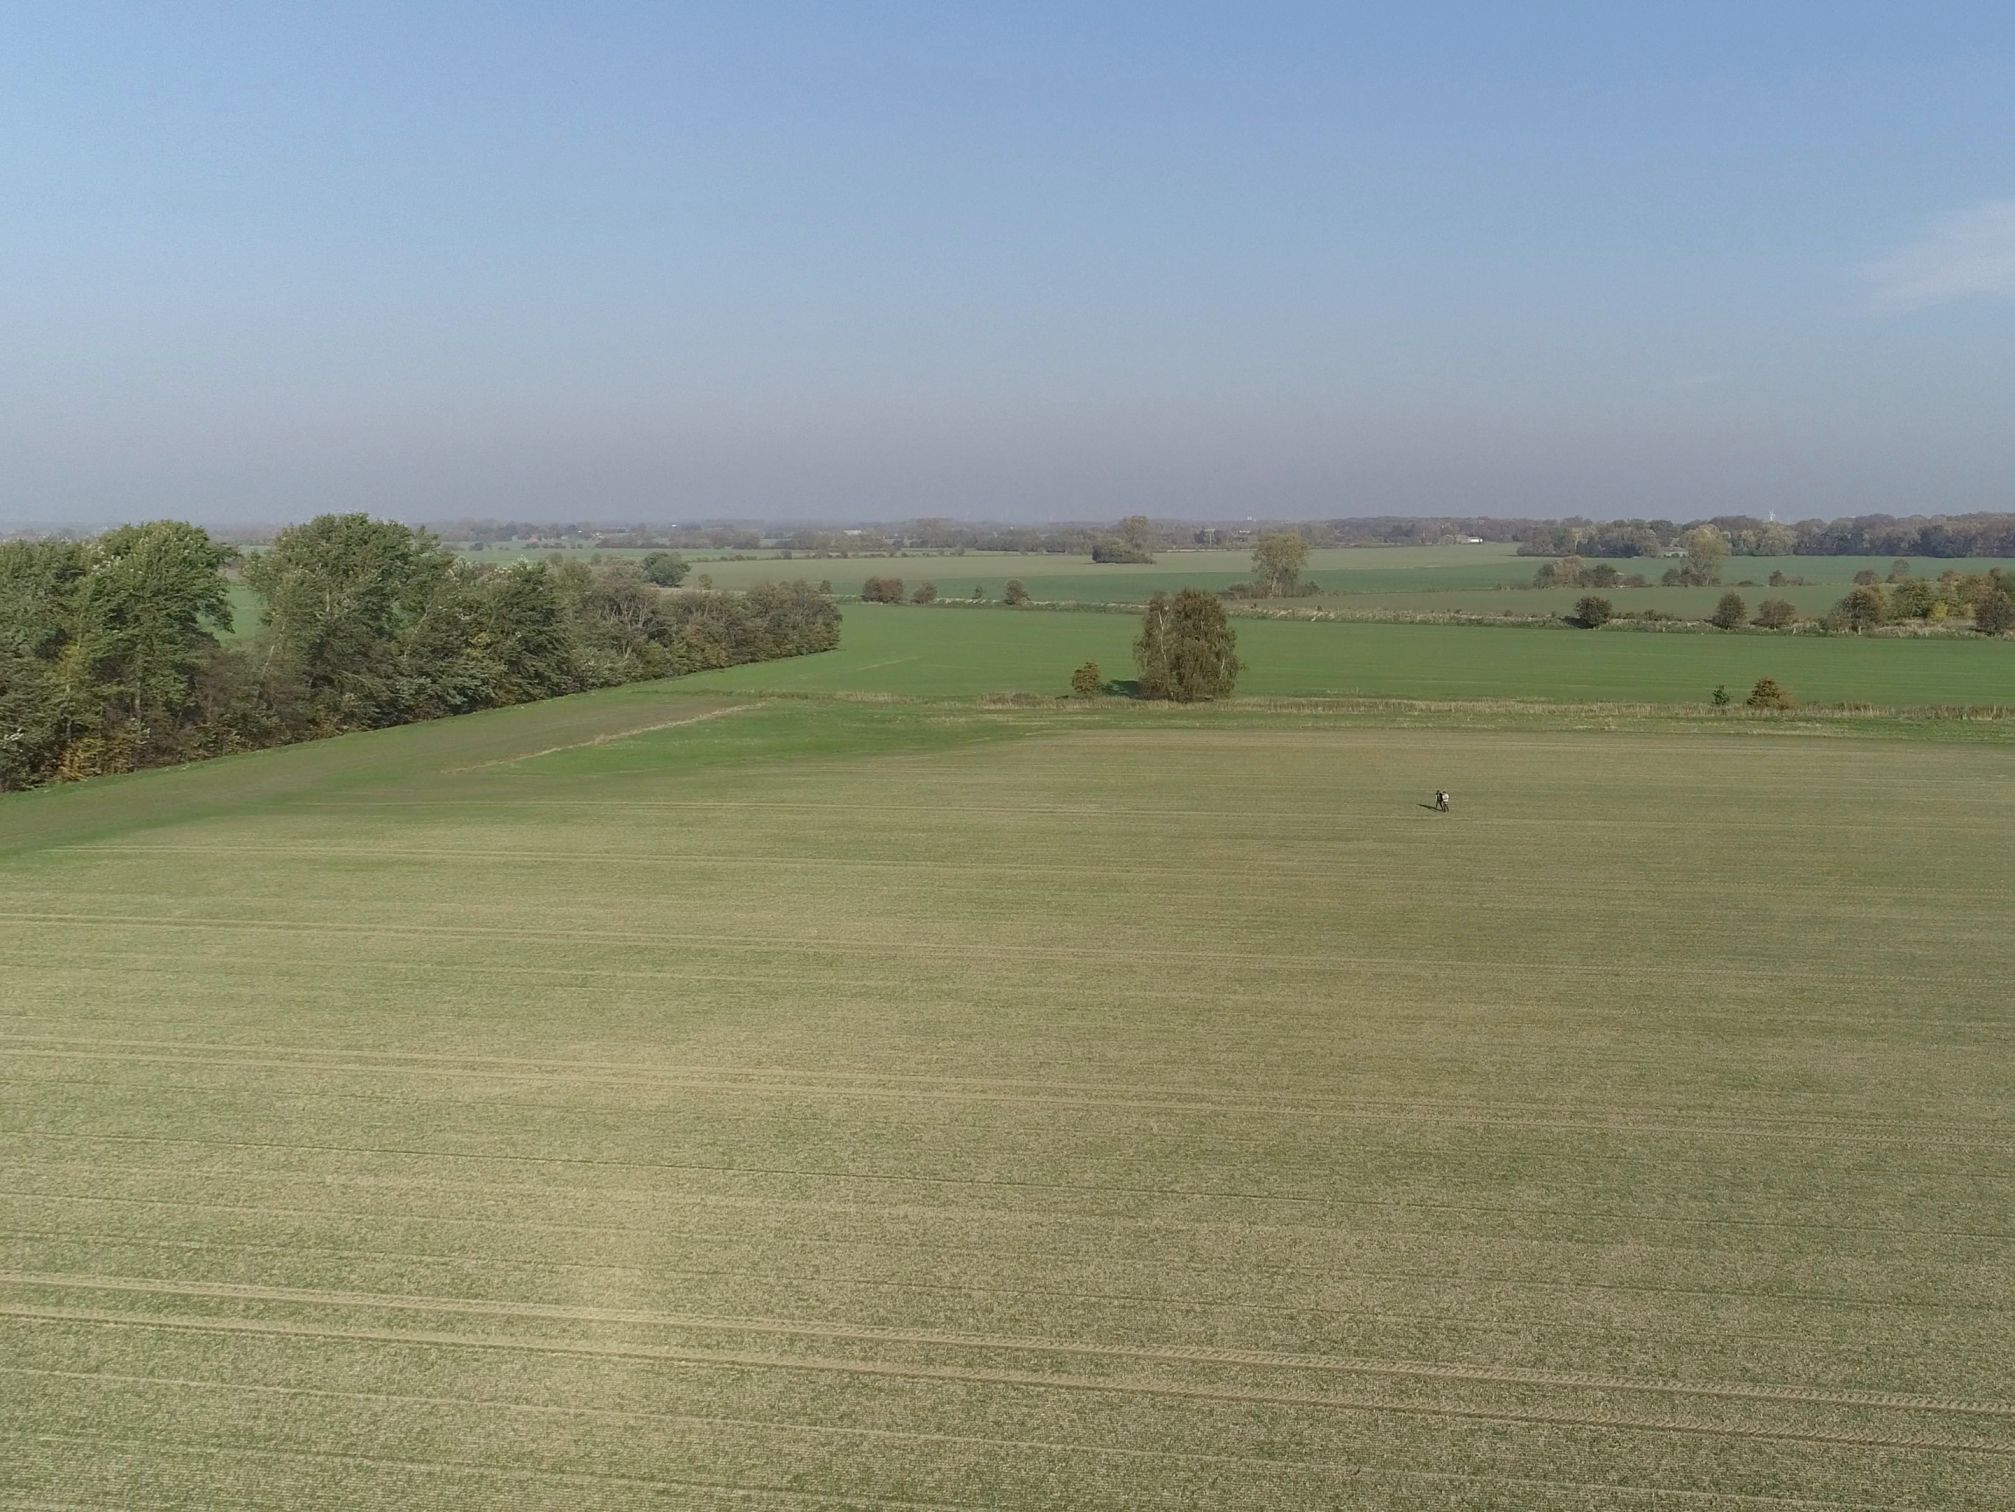
\includegraphics[width=3.122in]{figures/source/out30(1)}};

\path[fill=foo,line join=round,fill opacity=0.35,line width=0.256pt] (0.0000,247.7590) -- (227.8430,146.1690) -- (403.2000,150.1500) -- (403.2000,273.8490) -- (0.0000,247.7590) -- cycle;

\path[draw=white,line join=round,line width=0.512pt] (19.6911,244.5640) -- (56.0711,227.9040);



\path[draw=white,line join=round,line width=0.512pt] (19.8503,205.9030) -- (19.8504,244.6440) -- (67.5301,247.1570);



\path[fill=white,line join=round,line width=0.160pt] (63.6000,244.7010) -- (65.5307,247.0370) -- (63.4689,249.0560) -- (69.3046,247.0560) -- (63.6000,244.7010) -- cycle;



\path[fill=white,line join=round,line width=0.160pt] (52.5130,227.1350) -- (55.3596,228.1760) -- (54.6000,230.9590) -- (58.6260,226.2860) -- (52.5130,227.1350) -- cycle;



\path[fill=white,line join=round,line width=0.160pt] (17.6441,209.5580) -- (19.8958,207.5300) -- (22.0002,209.5030) -- (19.7535,203.7580) -- (17.6441,209.5580) -- cycle;



\path[cm={{1.0,0.0,0.0,1.0,(13.0,267.0)}}] (0.0000,0.0000) node[above right] () {\color{white}$\mathcal{O}_W$};



\path[cm={{1.0,0.0,0.0,1.0,(69.0,259.0)}}] (0.0000,0.0000) node[above right] () {\color{white}$x$};



\path[cm={{1.0,0.0,0.0,1.0,(50.0,220.0)}}] (0.0000,0.0000) node[above right] () {\color{white}$y$};



\path[cm={{1.0,0.0,0.0,1.0,(10.0,203.0)}}] (0.0000,0.0000) node[above right] () {\color{white}$z$};

\end{tikzpicture}


  \caption[The covering problem in a precision agriculture scenario]{The covering problem in a precision agriculture scenario. The aerial robot has to cover an agricultural field that forms a polygon (blue/transparent area in the frame) and run some autonomous tasks {\scriptsize(photo credit: Amit Ferencz Appel)}.}
  \label{fig:plot2}
\end{figure}

In the remainder of this work, we refer to computational tasks that can be scheduled in an energy-aware fashion as computations, opposed to the other tasks with no significant effect on energy consumption. We assume the aerial robot runs the computations on the heterogeneous computing hardware. As an example, we refer to an aerial robot in a precision agriculture scenario (see \fref{fig:opterra}{Figure}), which covers an agricultural field. In abstract terms, the field is represented by a polygon (see \fref{fig:plot2}{Figure}) and the aerial robot detects some patterns on such polygon using a convolutional neural network (CNN). The aerial robot further communicates the position of a detected pattern to other, ground-based actors. Detecting the patterns usually involves heterogeneous computing elements (GPU\findex{GPU} and/or multiple CPU\findex{CPU} cores) and consumes a significant amount of energy as opposed to communication. Detection is a computation, while communication is an (energy-inexpensive) task.

We are interested in the energy optimization of the path and computations under uncertainty (atmospheric interferences) in-flight and refer to it as dynamic energy planning. Unlike most of the past mobile robotics planning literature, the approach that we propose plans these two aspects simultaneously. Such planning would find optimal tradeoffs\findex{tradeoffs} between the path, computations, and energy requirements. Current generic planning solutions for aerial robots do not plan the path and computations dynamically, nor are they energy-aware. They are often semi-autonomous: the path and computations are static and usually defined using planning software~\citep{daponte2019review}. Instances of the planning software include famous flight controllers~\citep{px4,papa}. Such a state of practice has prompted us to investigate the topics presented in this work. We will gradually propose a dynamic energy planning approach for aerial robots. It plans both the path and computations while the aerial robot is flying and its batteries draining. 

We formally define the robot planning problem after outlining the approach in the next section.


%%%%%%%%%%%%%%%%%%%%%%%%%%%%%%%%%
\section{Outline of the Approach}
\label{sec:outline}

In this work, we address the increasing demands for autonomy of modern aerial robots with a dynamic planning approach. The approach provides a simultaneous energy-aware plan of the path and a power-saving schedule of the computations. To this end, we first need a user-defined initial plan that is then replanned energy-wise using an energy model for future prediction. Later, an algorithm inputs the initial plan, estimates the state of the energy model, evaluates future energy consumption and replans parameters relative to the path and computations. The plan consists of different stages. At each stage, the aerial robot flies a path and executes some computations. Furthermore, it contains some additional parameters to alter the path and computations along with an energy budget. The alterations are bounded. There are path constraint sets that bound the path alterations and computations constraint sets, one per each computation, that bound computations alterations.

We use the concept of different stages to model complex paths. For instance, the path might contain multiple circles and lines. We will see such plan later in \fref{sec:flight-plan}{Section}. The approach guides the aerial robot on different paths (the plan is composed of) using vector field~\citep{de2017guidance}. The robot switches between the paths as soon as it reaches specific triggering points. 

The approach further relies on \powprof{}, a profiling and modeling tool that we introduce in \fref{sec:comp-ener-model}{Section}. The tool models the energy consumption of the computations and is later employed to estimate the future energy of the aerial robot flying. To this end, we empirically derive and formally prove a periodic energy model that accounts for the uncertainty. We use Fourier analysis to derive the model and state estimation to address the uncertainty. Periodicity is often present due to repetitive patterns in the plan~\citep{seewald2020mechanical}. Indeed, mobile robots often iterate over a set of tasks and paths~\citep{seewald2021energy}. Given that the plan is periodic, we expect the energy consumption to evolve (approximately) periodically. We describe in detail such model in \fref{sec:periodic-model}{Section}. 

The replanning of the path and computations is achieved with modern optimal control techniques, such as optimal state estimation in \fref{cp:est}{Chapter}, and  model predictive control (MPC)~\citep{rawlings2017model} in \fref{cp:opt}{Chapter}. The control is data-driven. Energy sensor data estimates some coefficients of the model used to predict the future energy consumption with uncertainty. The replanning is done under an energy budget--the battery capacity and other battery parameters. Our goal is to complete the plan with the highest possible parameters configuration as the mobile robot executes the plan. 


%%%%%%%%%%%%%%%%%%%%%%
\section{Applications}

The dynamic energy planning in this work applies to modern aerial robots with a certain degree of autonomy. By the latter, we mean that the robot performs at least a predefined set of tasks over a given space. Although most of the guidance in \fref{cp:gd}{Chapter} is designed for aerial robots specifically, the approach can be easily adapted to other mobile robots with energy constraints. We discuss applications out of aerial robotics domain further in \fref{cp:conc}{Chapter}. For instance, we have applied the approach to the space robotics context~\citep{seewald2020beyond}. 

In the remainder of this work, we focus on the precision agriculture scenario in \fref{fig:plot2}{Figure}. In summary, the aerial robot covers a given agricultural field (a polygon) and searches for ground hazards. With the scenario, we validated the work experimentally. Path-wise, the aerial robot flies in circles and lines covering the polygon. Computation-wise, it detects hazards using the CNN and notifies grounded mobile robots employed for, e.g., harvesting. The approach alters the plan; it controls the processing rate and the radius of the circles affecting the distance between the lines. We will see this concrete scenario described formally in \fref{sec:flight-plan}{Section} and solved progressively in the remaining chapters.

%We observe that not only the path but also the computations significantly impact the energy, with a potential extension of up to 13 minutes over an hour by switching from the highest to the lowest level of computations in presence of a standard battery.

\section{Problem Formulation}
\label{sec:pb-form}

We formulate the mobile robot planning problem in \fref{sec:plan-pb}{Section}. Before we provide a formal definition of some basic constructs in \fref{sec:definitions}{Sections}\fref{sec:plan}{--\hspace*{-.8ex}}. We then provide a formal example of the precision agriculture scenario in \fref{sec:flight-plan}{Section}.

\subsection{Definitions of computations and motion}
\label{sec:definitions}

Firstly, we define computations, motion, their energy, and M\&CE.

\begin{highlight}
  \begin{defn}[Computations/motion]\label{def:comps}
    Computations are energy-demanding computational tasks. The mobile robot runs the computations on heterogeneous computing hardware. The computing hardware interface microcontrollers.
    
    Motion is the act of the mobile robot moving in the surrounding environment. The mobile robot runs some primitives on microcontrollers for this purpose. The microcontrollers interface actuators, motors, and other components.%The primitives often originate from the computing hardware.
  \end{defn}
\end{highlight}

Autonomous capabilities are achieved by interconnecting heterogeneous computing hardware and microcontrollers. We assume that for the computations, the heterogeneous computing hardware runs a schedule. The schedule is then characterized by some parameters. For instance, for the CNN detection from the precision agriculture scenario, a parameter is the frames per second (\Gls{acr:fps})\findex{frames per second} rate. Alike for the computations, we assume that for the motion, the robot travels some paths characterized by some other parameters. For instance, for the covering problem, a parameter changes the distance between the survey lines.

\begin{highlight}
\begin{defn}[Computations/motion energy]\label{def:comp-mot-energy}
  Given a schedule characterized by parameters $c_i^\sigma:=\{c_{i,\rho+1},\dots,c_{i,\rho+\sigma}\}$, the computations energy is the energy spent by heterogeneous computing hardware executing the schedule.
  
  Given a path characterized by $\rho$ parameters $c_i^\rho:=\{c_{i,1},c_{i,2},\dots,c_{i,\rho}\}$, the motion energy is the energy spent by the mobile robot while moving on the path.
\end{defn}
\end{highlight}

Physically, the motion energy is the energy spent by all the systems powering the mobile robot, excluding the heterogeneous computing hardware. Computations energy and motion energy are measured in watts for instantaneous or average measures. They are measured in joules for measures over a given time interval. We show in \fref{sec:defs-stages-triggs}{Section} what we mean by characterization of path and computations with some parameters and illustrate the concept on an example in \fref{sec:flight-plan}{Section}. 

\Gls{acr:mace}\findex{difference of motion and computations energy} that we introduced in \fref{sec:aerial-robo-types}{Section} is the difference of average motion and computations energy. It is measured in watts, and it gives a measure of which of the two energy components is predominant. For \Gls{acr:mace} greater than zero, the motion energy dominates over the computations. The dynamic planning approach plans first an energy-efficient path. This is the case for rotary-wing aerial robots \sref{lab:matrice}, and \sref{lab:agras} in \fref{fig:plot10}{Figure}. For \Gls{acr:mace} lower than zero, the computations energy dominates. The dynamic planning approach plans first a power-saving schedule. It is the case for lighter-than-air aerial robot \sref{lab:skye} in \fref{fig:plot10}{Figure}. For \Gls{acr:mace} close to zero, both energy components are important energy-wise. The dynamic planning approach plans both an energy-efficient path and power-saving schedule to a similar extent. This M\&CE is characteristic for fixed-wing aerial robots \sref{lab:cumulus}\fref{lab:opterra}{--\hspace*{-.8ex}} in \fref{fig:plot10}{Figure}.

\subsection{Definitions of path functions}
\label{sec:path-functions}

To model the path we use multiple mathematical functions $\varphi_1,\varphi_2,\dots$ that we call path functions. These functions express the path in 2D at a fixed altitude $h$. 

\begin{highlight}
  \begin{defn}[Path functions]\label{def:paths}
    The functions $\varphi_i:\mathbb{R}^2\rightarrow\mathbb{R}$ are the path functions $\forall i\in\{1,2,\dots\}$. They quantify the distance of a generic point $\mathbf{p}:=(x_{\mathbf{p}},y_{\mathbf{p}})$ in the 2D space on the $z$-axis from $\varphi_i=0$ and are continuous and twice differentiable. 
  \end{defn}
\end{highlight}

\begin{figure}[t]
  \centering
  
\definecolor{cECECEC}{RGB}{236,236,236}
\definecolor{c989898}{RGB}{152,152,152}


\def \globalscale {1.000000}
\begin{tikzpicture}[y=0.80pt, x=0.80pt, yscale=-.9*\globalscale, xscale=.9*\globalscale, inner sep=0pt, outer sep=0pt]
\path[fill=cECECEC,line join=round,line width=0.160pt] (338.3020,263.8010) -- (381.1050,-0.0001) -- (102.8640,12.1601) -- (58.1440,275.9610) -- (338.3020,263.8010) -- cycle;



\path[draw=c989898,line join=round,line width=0.512pt] (147.6250,213.3720) -- (173.5250,186.3120) -- (132.2780,180.7850);



\path[fill=c989898,line join=round,line width=0.256pt] (163.3290,190.5470) -- (158.3650,192.4980) -- (158.1310,191.9020) -- (163.0950,189.9520) -- (163.3290,190.5470) -- cycle(153.4020,194.4490) -- (148.4380,196.4000) -- (148.2040,195.8040) -- (153.1680,193.8530) -- (153.4020,194.4490) -- cycle(143.4740,198.3510) -- (138.5110,200.3020) -- (138.2760,199.7060) -- (143.2400,197.7550) -- (143.4740,198.3510) -- cycle(133.5470,202.2530) -- (128.5830,204.2040) -- (128.3490,203.6080) -- (133.3130,201.6570) -- (133.5470,202.2530) -- cycle(123.6200,206.1550) -- (118.6560,208.1060) -- (118.4220,207.5100) -- (123.3850,205.5590) -- (123.6200,206.1550) -- cycle(113.6920,210.0560) -- (108.7280,212.0070) -- (108.4940,211.4120) -- (113.4580,209.4610) -- (113.6920,210.0560) -- cycle(103.7650,213.9580) -- (100.0090,215.4350) -- (99.7748,214.8390) -- (103.5310,213.3630) -- (103.7650,213.9580) -- cycle(173.2570,186.6450) -- (168.2930,188.5960) -- (168.0590,188.0010) -- (173.0220,186.0500) -- (173.2570,186.6450) -- cycle;



\path[draw=c989898,line join=round,line width=0.512pt] (55.1846,208.3180) -- (99.4269,215.2590);



\path[draw=black,line join=round,line width=0.512pt] (68.2145,216.7950) -- (99.1080,215.5400);



\path[draw=c989898,line join=round,line width=0.512pt] (99.5793,215.0880) -- (196.7320,112.9950);



\path[draw=foo,line join=round,line width=0.512pt] (139.9040,221.4650) -- (147.6230,213.4870);



\path[draw=black,line join=round,line width=0.512pt] (99.6097,215.3190) -- (377.1250,258.8550);



\path[fill=foo,line join=round,line width=0.256pt] (163.7520,67.1159) -- (158.7880,69.0661) -- (158.5540,68.4704) -- (163.5180,66.5202) -- (163.7520,67.1159) -- cycle(153.8240,71.0164) -- (148.8600,72.9667) -- (148.6260,72.3709) -- (153.5900,70.4207) -- (153.8240,71.0164) -- cycle(143.8960,74.9168) -- (138.9320,76.8670) -- (138.6980,76.2713) -- (143.6620,74.3211) -- (143.8960,74.9168) -- cycle(133.9680,78.8173) -- (129.0040,80.7676) -- (128.7700,80.1719) -- (133.7340,78.2216) -- (133.9680,78.8173) -- cycle(124.0400,82.7178) -- (119.0760,84.6679) -- (118.8420,84.0722) -- (123.8060,82.1220) -- (124.0400,82.7178) -- cycle(114.1120,86.6182) -- (109.1480,88.5685) -- (108.9140,87.9728) -- (113.8780,86.0225) -- (114.1120,86.6182) -- cycle(104.1840,90.5187) -- (99.9651,92.1761) -- (99.7311,91.5804) -- (103.9500,89.9230) -- (104.1840,90.5187) -- cycle(173.6800,63.2155) -- (168.7160,65.1657) -- (168.4820,64.5700) -- (173.4460,62.6198) -- (173.6800,63.2155) -- cycle;



\path[draw=black,line join=round,line width=0.512pt] (99.6194,255.8350) -- (99.6701,45.2765);



\path[fill=black,line join=round,line width=0.160pt] (97.4234,50.0749) -- (99.6963,48.0699) -- (101.7800,50.0657) -- (99.5939,44.2973) -- (97.4234,50.0749) -- cycle;



\path[fill=black,line join=round,line width=0.160pt] (372.7840,255.6340) -- (374.2970,258.2610) -- (371.9260,259.9050) -- (378.0140,258.9110) -- (372.7840,255.6340) -- cycle;



\path[draw=c989898,fill=c989898,line join=round,line width=0.160pt] (191.9960,115.1180) -- (195.0250,115.0410) -- (195.3410,117.9090) -- (197.3700,112.0830) -- (191.9960,115.1180) -- cycle;



\path[draw=black,line join=round,line width=0.512pt] (99.6614,215.4240) -- (348.2110,205.3130);



\path[fill=black,line join=round,line width=0.256pt] (365.8960,204.3560) -- (371.2240,204.1220) -- (371.2520,204.7610) -- (365.9240,204.9950) -- (365.8960,204.3560) -- cycle(376.5520,203.8870) -- (381.8800,203.6530) -- (381.9080,204.2920) -- (376.5800,204.5270) -- (376.5520,203.8870) -- cycle(387.2080,203.4190) -- (391.6130,203.2250) -- (391.6410,203.8640) -- (387.2370,204.0580) -- (387.2080,203.4190) -- cycle(355.2390,204.8250) -- (360.5670,204.5900) -- (360.5960,205.2300) -- (355.2670,205.4640) -- (355.2390,204.8250) -- cycle;



\path[fill=black,line join=round,line width=0.256pt] (51.6916,217.8380) -- (46.3616,218.0290) -- (46.3388,217.3890) -- (51.6687,217.1990) -- (51.6916,217.8380) -- cycle(41.0317,218.2190) -- (35.7017,218.4090) -- (35.6789,217.7700) -- (41.0088,217.5790) -- (41.0317,218.2190) -- cycle(30.3718,218.6000) -- (25.0419,218.7900) -- (25.0190,218.1500) -- (30.3490,217.9600) -- (30.3718,218.6000) -- cycle(62.3514,217.4570) -- (57.0215,217.6480) -- (56.9986,217.0080) -- (62.3286,216.8180) -- (62.3514,217.4570) -- cycle;



\path[draw=black,line join=round,line width=0.512pt] (138.1150,223.3150) -- (140.0590,221.3710);



\path[draw=c989898,line join=round,line width=0.512pt] (129.6630,180.5070) -- (132.3930,180.8300);



\path[draw=c989898,line join=round,line width=0.512pt] (173.5260,186.3500) -- (173.5730,63.0377);



\path[draw=black,line join=round,line width=0.512pt] (96.7492,91.8181) -- (99.4988,91.8249);



\path[cm={{1.0,0.0,0.0,1.0,(376.0,276.0)}}] (0.0000,0.0000) node[above right] () {$x$};



\path[cm={{1.0,0.0,0.0,1.0,(198.0,102.0)}}] (0.0000,0.0000) node[above right] () {$y$};



\path[cm={{1.0,0.0,0.0,1.0,(85.0,46.0)}}] (0.0000,0.0000) node[above right] () {$z$};



\path[draw=black,line join=round,line width=0.512pt] (83.3760,232.1090) -- (99.6032,215.0620);



\path[fill=c989898,line join=round,line width=0.512pt] (173.2360,184.7230) .. controls (174.0900,184.7230) and (174.7820,185.4150) .. (174.7820,186.2700) .. controls (174.7820,187.1240) and (174.0900,187.8160) .. (173.2360,187.8160) .. controls (172.3810,187.8160) and (171.6890,187.1240) .. (171.6890,186.2700) .. controls (171.6890,185.4150) and (172.3810,184.7230) .. (173.2360,184.7230) -- cycle;



\path[cm={{1.0,0.0,0.0,1.0,(161.0,289.0)}}] (0.0000,0.0000) node[above right] () {$\varphi(x,y):=2y-x$};



\path[cm={{1.0,0.0,0.0,1.0,(353.0,224.0)}}] (0.0000,0.0000) node[above right] () {$2y-x=0$};



\path[cm={{1.0,0.0,0.0,1.0,(131.0,238.0)}}] (0.0000,0.0000) node[above right] () {$x_\mathbf{p}$};



\path[cm={{1.0,0.0,0.0,1.0,(113.0,180.9)}}] (0.0000,0.0000) node[above right] () {$y_\mathbf{p}$};



\path[cm={{1.0,0.0,0.0,1.0,(41.0,98.0)}}] (0.0000,0.0000) node[above right] () {$\varphi(\mathbf{p})=d$};



\path[draw=c989898,fill=c989898,line join=round,line width=0.160pt] (175.7670,179.7880) -- (173.4940,181.7930) -- (171.4110,179.7970) -- (173.5970,185.5660) -- (175.7670,179.7880) -- cycle;



\path[draw=c989898,fill=c989898,line join=round,line width=0.160pt] (171.2840,70.1412) -- (173.5570,68.1363) -- (175.6400,70.1321) -- (173.4540,64.3637) -- (171.2840,70.1412) -- cycle;



\path[fill=foo,line join=round,line width=0.512pt] (173.4160,61.7418) .. controls (174.2700,61.7418) and (174.9630,62.4342) .. (174.9630,63.2885) .. controls (174.9630,64.1427) and (174.2700,64.8351) .. (173.4160,64.8351) .. controls (172.5620,64.8351) and (171.8700,64.1427) .. (171.8700,63.2885) .. controls (171.8700,62.4342) and (172.5620,61.7418) .. (173.4160,61.7418) -- cycle;



  \path[fill=cECECEC,line join=round,line width=0.160pt] (182.5940,102.1690) -- (164.2430,102.1690) -- (164.1940,119.9680) -- (182.5870,119.9220) -- (182.5940,102.1690) -- cycle;



  \path[cm={{1.0,0.0,0.0,1.0,(170.0,116.0)}}] (0.0000,0.0000) node[above right] () {$d$};



\path[cm={{1.0,0.0,0.0,1.0,(187.0,186.0)}}] (0.0000,0.0000) node[above right] () {$(x_\mathbf{p},y_\mathbf{p},0)$};




\end{tikzpicture}


  \caption[Concept of the path and generic point in space]{The path defined as mathematical function $\varphi=h$ at a fixed altitude $h$. A generic point $\mathbf{p}$ in 2D space quantifies the distance $\varphi(\mathbf{p})=d$ on the $z$-axis from $h$.}
  \label{fig:plot1}
\end{figure}

We use this notion to guide the aerial robot using a vector field in \fref{cp:gd}{Chapter}. For instance, one can define a line
\begin{equation}\label{eq:basic-path}
  \varphi(x,y):=ax+by+c,
\end{equation}
where $a,b,c\in\mathbb{R}$ are given constants. A generic point $\mathbf{p}:=(x_{\mathbf{p}},y_{\mathbf{p}})$ intersects $\varphi(x,y)$ on a specific value of the $z$-axis. The concept is illustrated in \fref{fig:plot1}{Figure} for $c$ zero and $a,b$ minus one and two respectively. A generic point $\mathbf{p}$ intersects the plane
\begin{equation}
  \varphi(x,y):=2y-x,
\end{equation}
at $z=\varphi(\mathbf{p})$. The path at a fixed altitude is then $\varphi(x,y)=0$, or more generally $\varphi(x,y)=h$ with $h\in\mathbb{R}$. $\varphi(\mathbf{p})-h$ is then the distance on $z$-axis.

In this work, we use lines and circles as path functions. We connect these functions using some specific points--the triggering points. However, one can define any mathematical function, with the only requirement being continuity and twice differentiability. We use the first derivative for the vector field, the second derivative to derive the control action. We explain both derivatives further in \fref{cp:gd}{Chapter}.

\subsection{Definitions of stages and triggering points}
\label{sec:defs-stages-triggs}

%To specify an integer-valued set, we relay on the following mathematical notation: $[x]$ is the set positive set $\{0,1,\dots,x\}\subseteq\mathbb{Z}_{\geq 0}$, where $x\in\mathbb{Z}_{\geq 0}$. $[x]_{>0}$ is the strictly positive set $\{1,2,\dots,x\}\subseteq\mathbb{Z}_{> 0}$ (or $[x]/\{0\}$). where $x\in\mathbb{Z}_{>0}$. 

%Bold lower-case letters, such as $\mathbf{x}$, denote vectors. Upper-case letters, such as $X$, denote matrices.

Parameters are real- $\mathbb{R}$ or integer-valued $\mathbb{Z}$ variable values. We use the parameters to dynamically plan the path and computations, since they influence the computations/motion energy in \fref{def:comp-mot-energy}{Definition}. We use the notation  $c_{i,j}$ to denote the $j$-th parameter of the $i$-th parameters set $c_i$
\begin{equation}
  c_i=\{c_{i,1},c_{i,2},\dots,c_{i,j},\dots\}.
\end{equation}

The user-defined plan has a number of stages $i=\{1,2,\dots\}$, and we assume that at each stage $i$ the mobile robot runs a schedule and travels a path function $\varphi_i$ using the parameters set $c_i$. Parameters are bounded. $\underline{c}_{i,j}$ is the lower bound of the parameter $c_{i,j}$. $\overline{c}_{i,j}$ is the upper bound
\begin{equation}
  \underline{c}_{i,j}\leq c_{i,j}\leq\overline{c}_{i,j}.
\end{equation}

We assume there are $\rho$ \emph{path}-specific \emph{parameters}\findex{path parameters} and $\sigma$ \emph{computations}-specific \emph{parameters}\findex{computations parameters} for every stage. This means that the path at stage $i$ can be replanned with $\rho$ path parameters
$c_i^\rho:=\{c_{i,1},c_{i,2},\dots,c_{i,\rho}\}$,
while the computations (i.e., the energy-demanding computational task executed on heterogeneous computing hardware in \fref{def:comps}{Definition}) with $\sigma$ computation parameters 
$c_i^\sigma:=\{c_{i,\rho+1},c_{i,\rho+2},\dots,c_{i,\rho+\sigma}\}$.

Returning to \fref{sec:path-functions}{Section}, by characterization of the path with parameters, we mean that we enhance $\varphi_i$ with the path parameters $c_i^\rho$. $\varphi_i:\mathbb{R}^2\times\mathbb{R}^\rho\rightarrow\mathbb{R}$ is thus a (continuous twice differentiable) function of a point and the path parameters. The parameters are used to alter the path and thus change the energy consumption.
Similarly, by characterization of the schedule with parameters, we mean that we express the computations as the value of the computation parameters. These are also employed for the purpose of energy alteration by, e.g., decreasing the granularity of a given computation and thus lowering instantaneous energy consumption. We discuss the alteration of the energy with path parameters and computation parameters further in \fref{sec:nom-cont}{Section} and \fref{sec:merging}{Section}.

We formally define the stage in \fref{def:stage}{Definition}.

\begin{highlight}  
  \begin{defn}[Stage]\label{def:stage}
    Given $\mathbf{p}(t)$, a point of a mobile robot travelling at an altitude $h\in\mathbb{R}_{\geq 0}$ with respect to an inertial navigation frame $\mathcal{O}_W$, the $i$-th \emph{stage}\findex{stage} $\Gamma_i$ at time instant $t$ of a plan $\Gamma$ is
    \begin{equation*}\begin{split}
      \Gamma_i:=\{\varphi_i(\mathbf{p}(t),c_i^\rho),c_i^\sigma\mid
      \,&\forall j\,\in\,[\rho]_{>0},\,c_{i,j}\,\,\,\,\,\,\,\in\mathcal{C}_{i,j},\,\\
        &\,\forall k\in[\sigma]_{>0},\,c_{i,\rho+k}\in\mathcal{S}_{i,k}\,\},
    \end{split}\end{equation*}
    where $\mathcal{C}_{i,j}:=[\underline{c}_{i,j},\overline{c}_{i,j}]\subseteq\mathbb{R}$ is the $j$-th path parameter constraint set, and $\mathcal{S}_{i,k}:=[\underline{c}_{i,\rho+k},\overline{c}_{i,\rho+k}]\subseteq\mathbb{Z}_{\geq 0}$ the $k$-th computation parameter constraint set.
  \end{defn}
\end{highlight}

We note that the altitude $h$ from \fref{def:stage}{Definition} is not strictly fixed. It might change at different flying phases, and under different atmospheric conditions. Furthermore, we merge the computation constraint sets and the path constraint set in a single constraint set for simplicity. The constraint set for the $i$-th stage
\begin{equation}\label{eq:constraint-set}
  \mathcal{U}_i:=\begin{cases}
  \mathcal{C}_{i,j} & \text{for } c_{i,j} \text{ with } j\leq\rho\\
  \mathcal{S}_{i,j-\rho} & \text{for } c_{i,j} \text{ with } \rho<j\leq\sigma
\end{cases}.\end{equation}

To move from a given stage $\Gamma_i$ to the next stage $\Gamma_{i+1}$, we define some specific points. As soon as the mobile robot reaches the proximity of these points, it switches to the next stage.

\begin{highlight}  
  \begin{defn}[Triggering, and final point]\label{def:trigs}
    The point $\mathbf{p}_{\Gamma_{i}}$ that allows the transition between $\Gamma_i$ and $\Gamma_{i+1}$ is called \emph{triggering point}. The last triggering point $\mathbf{p}_{\Gamma_{l}}$ relative to the last stage $\Gamma_l$ is called \emph{final point}.
  \end{defn}
\end{highlight}

\subsection{Definition of the plan}
\label{sec:plan}

We now define the plan in \fref{def:plan}{Definition} as a finite state machine using the constructs of path functions in \fref{def:paths}{Definition}, stages and triggering points in \fref{def:stage}{Definitions}\fref{def:trigs}{--\hspace*{-.8ex}}.

\begin{highlight}  
  \begin{defn}[Plan]\label{def:plan}
    Given $\mathbf{p}(t)$ from \fref{def:stage}{Definition}, the \emph{plan} is a finite state machine\findex{finite state machine} (\Gls{acr:fsm}) $\Gamma$, where the state-transition function $s:\bigcup_i{\Gamma_i}\times\mathbb{R}^2\rightarrow\bigcup_i{\Gamma_i}$ maps a stage and a point to the next stage
    \begin{equation*}s(\Gamma_i,\mathbf{p}(t)):=\begin{cases}
      \Gamma_{i+1} & \text{if }\mathbf{p}(t)=\mathbf{p}_{\Gamma_i}\\
      \Gamma_i & \text{otherwise}
    \end{cases}.\end{equation*}
  \end{defn}
\end{highlight}

We illustrate the definition of plan, stage, trigerring, and final points in \fref{fig:state-machine}{Figures}\fref{fig:state-machine2}{--\hspace*{-.8ex}}.

\begin{figure}[h!]
  \center
  \begin{tikzpicture}[shorten >=.5pt,node distance=12.5ex,on grid,auto,initial text=\footnotesize\fontfamily{phv}\selectfont{start}]
    \node[state,initial] (q_i) {$\Gamma_1$}; 
    \node        [right=of q_i] (q_dots0) {$\cdots$};
    \node[state] (q_0) [right=of q_dots0] {$\Gamma_i$};
    \node        (q_dots1) [right=of q_0] {$\cdots$};
    \node[state,accepting] (q_f) [right=of q_dots1] {$\Gamma_f$};
    \path[->]
    (q_i) edge node {$\mathbf{p}_{\Gamma_{1}}$} (q_dots0)
    (q_dots0) edge node{$\mathbf{p}_{\Gamma_{i-1}}$} (q_0)
    (q_0) edge node {$\mathbf{p}_{\Gamma_i}$} (q_dots1)
    (q_dots1) edge node {$\mathbf{p}_{\Gamma_{l}}$} (q_f)    
    (q_i) edge [loop above] node {$\mathbf{p}(t_1)$} (q_i)
    (q_0) edge [loop above] node {$\mathbf{p}(t_2)$} (q_0)
    (q_f) edge [loop above] node {$\mathbf{p}(t_3)$} (q_f)
    ; %end path 
    \draw [decorate,decoration={brace,amplitude=10pt,mirror,raise=10pt},yshift=0pt]
    (q_i.south west) -- (q_f.south west) node [black,midway,yshift=-9ex]{$\Gamma$};
  \end{tikzpicture}
  \caption[Definition of a plan]{Definition of a plan $\Gamma$ as an FSM. Each state is a stage $\Gamma_i$, the transition happens in proximity of specific points called triggering points $\mathbf{p}_{\Gamma_i}$. The accepting stage $\Gamma_f$ indicates the termination of the plan.}
  \label{fig:state-machine}
\end{figure}
In \fref{fig:state-machine}{Figure} we illustrate a simple linear plan. The triggering point $\mathbf{p}_{\Gamma_{i-1}}$ allows the transition to the stage $\Gamma_i$. The robot remains in the stage with any generic point $\mathbf{p}(t_2)$. It eventually enters the stage $\Gamma_{i+1}$ with the triggering point $\mathbf{p}_{\Gamma_i}$ and so on, until it reaches the final point. $\Gamma_f$ is the accepting stage (it indicates that the robot has completed the plan).
\begin{figure}[h!]
  \center
  \begin{tikzpicture}[shorten >=1pt,node distance=27ex,on grid,auto]
    \node        (q_dots0) {$\cdots$};
    \node[state] (q_0) [right=of q_dots0] {$\Gamma_i$};
    \node        (q_dots1) [right=of q_0] {$\cdots$};   
    \path[->]
    (q_dots0) edge node{$\mathbf{p}_{\Gamma_{i-1}}(c_1^\rho,\dots,c_{i-1}^\rho)$} (q_0)
    (q_0) edge node {$\mathbf{p}_{\Gamma_i}(c_1^\rho,\dots,c_{i}^\rho)$} (q_dots1)    
    (q_0) edge [loop above] node {$\mathbf{p}(t_2)$} (q_0)
    ; %end path
  \end{tikzpicture}
\caption[Detail of a stage in the FSM]{Detail of the stage $\Gamma_i$ in the FSM. The triggering points used to transition between stages (states in the FSM) are expressed in function of the last and/or previous triggering points.}
\label{fig:state-machine2}
\end{figure}
In \fref{fig:state-machine2}{Figure} we illustrate that generally, one can express the triggering points in function of the $i$-th trajectory parameters $c_{i}^{\rho}$, or any previous trajectory parameters, propagating the information therein if necessary. We further expand on this notion in the example in \fref{sec:flight-plan}{Section}. 

In order to simplify the planning problem, we consider some \emph{primitive paths}\findex{primitive paths}. All the other paths are built from these paths with a shift $\mathbf{d}:=(x_{\mathbf{d}},y_{\mathbf{d}})$. 

Let us suppose the plan is composed of $l$ stages. Given $n\in\mathbb{Z}_{>0}$ ($n<l,l/n\in\mathbb{Z}$) primitive paths $\varphi_1,\dots\varphi_n$, a generic starting point $\mathbf{p}(t_0)$ at the initial time $t_0$, and the current levels of the path parameters $c_1^\rho$, all the other paths $\varphi_{n+1},\dots,\varphi_l$ are built
\begin{equation}\label{eq:primitive}\begin{split}
  &\varphi_{(i-1)n+j}(\mathbf{p}+(i-1)\mathbf{d},c_1^\rho)-\varphi_{in+j}(\mathbf{p}+i\mathbf{d},c_1^\rho)=e_j,
\end{split}\end{equation}
$\forall i\in[l/n-1]^+,j\in[n]^+$, where $e_j\in\mathbb{R}$ is the $j$-th constant difference.

\begin{figure}[h!]
  \center
  \begin{tikzpicture}[shorten >=.5pt,node distance=12.5ex,on grid,auto,initial text=\footnotesize\fontfamily{phv}\selectfont{start}]
    \node[state,initial] (q_i) {$\Gamma_1$}; 
    \node[state] (q_2) [right=of q_i] {$\Gamma_2$}; 
    \node        [right=of q_2] (q_dots0) {$\cdots$};
    \node[state] (q_0) [right=of q_dots0] {$\Gamma_n$};
    \node[state,accepting] (q_f) [right=of q_0] {$\Gamma_f$};
    \path[->]
    (q_i) edge node {$\mathbf{p}_{\Gamma_{1}}$} (q_2)
    (q_2) edge node {$\mathbf{p}_{\Gamma_{2}}$} (q_dots0)
    (q_dots0) edge node{$\mathbf{p}_{\Gamma_{n-1}}$} (q_0)
    (q_0) edge [bend right=65] node [above] {$\mathbf{p}_{\Gamma_n}$} (q_i)
    (q_i) edge [bend left=-65] node [above] {$\mathbf{p}_{\Gamma_l}$} (q_f)
    (q_2) edge [bend left=-45] node [above] {$\mathbf{p}_{\Gamma_l}$} (q_f)
    (q_0) edge node {$\mathbf{p}_{\Gamma_{l}}$} (q_f)    
    (q_i) edge [loop above] node {$\mathbf{p}(t_1)$} (q_i)
    (q_2) edge [loop above] node {$\mathbf{p}(t_2)$} (q_2)
    (q_0) edge [loop above] node {$\mathbf{p}(t_3)$} (q_0)
    (q_f) edge [loop above] node {$\mathbf{p}(t_4)$} (q_f)
    ; %end path 
    \draw [decorate,decoration={brace,amplitude=10pt,mirror,raise=60pt},yshift=0pt]
    (q_i.south west) -- (q_f.south west) node [black,midway,yshift=-22ex]{$\Gamma$};
  \end{tikzpicture}
  \caption[Definition of a plan with a loop]{Definition of a plan $\Gamma$ that contain a loop. Stages $\Gamma_1,\Gamma_2,\dots,\Gamma_i$ containing primitive paths $\varphi_1,\varphi_2,\dots,\varphi_n$ are iterated with a shift $\mathbf{d}$.}
  \label{fig:state-machine-loop}
\end{figure}
In \fref{fig:state-machine-loop}{Figure} we illustrate a plan composed of $n$ primitive stages $\Gamma_1,\Gamma_2,\dots,\Gamma_n$ (containing primitive paths $\varphi_1,\varphi_2,\dots,\varphi_n$) that are reiterated with the shift $\mathbf{d}$.

An important concept for the energy estimation is the concept of period--the time required to fly the primitive paths $\varphi_1,\varphi_2,\dots,\varphi_n$ (or generally $\varphi_{(i-1)n+1},$ $\varphi_{(i-1)n+2},\dots,\varphi_{(i-1)n+n}$). 

\begin{highlight}
  \begin{defn}[Period]\label{def:period}\findex{period}
    The period $T\in\mathbb{R}_{> 0}$ is the time between $\varphi_{(i-1)n+j}$ and $\varphi_{in+j}$ in \frefeq{eq:primitive}.
  \end{defn} 
\end{highlight}
  
We assume the initial period is one and measure the period required to fly the paths physically or in simulation. The periods might be different for different $j$s due to atmospheric interferences. For the path functions, one can define the plan using primitive paths $\varphi_1,\varphi_2,\dots,\varphi_n$ or define all the stages explicitly and find $n$ searching the value which satisfies the \frefeq{eq:primitive}. If there is no such value, (e.g., when the plan is composed of only one stage or the plan is aperiodic), the period $T$ from \fref{def:period}{Definition} can be determined empirically from energy data or assumed as the total flight time. The latter eventuality has an effect on the energy model. We discuss the period estimation further in \fref{sec:period-est}{Section}.

\subsection{Planning problem}
\label{sec:plan-pb}

We now wrap all the constructs from the previous sections and define the planning problem.

\begin{highlight}
\begin{pb}[Planning problem]\label{pb}\findex{planning problem}
  Consider an initial plan $\Gamma$ from \fref{def:stage}{Definition}. We are interested in the planning of the path and computations parameters $c_i,\,\forall i\in[l]^+$ under energy constraints and uncertainty.
  
  We are further interested in the guidance to the path and the scheduling of the computations resulting from such planning.
\end{pb}    
\end{highlight}


---

\subsection{Precision agriculture example}
\label{sec:flight-plan}

In this section, we discuss an example of a plan for an autonomous aerial robot in a precision agriculture scenario addressing the covering problem in \fref{fig:plot2}{Figure}. We assume the polygon is regular and has four sides (it is a rectangle). An intuitive static plan $\Gamma$ can be composed of lines connected by circles. The distance between the lines can be then used as a measure of the quality of the coverage. Such intuitive static plan is illustrated in \fref{fig:plot3}{Figure}.

\begin{figure}[h]
  \centering
  
\def \globalscale {1.000000}
\begin{tikzpicture}[y=0.80pt, x=0.80pt, yscale=-\globalscale, xscale=\globalscale, inner sep=0pt, outer sep=0pt]
\path[fill=foo,line join=round,line width=0.256pt] (31.2248,223.3740) -- (36.5581,223.3740) -- (36.5581,224.0140) -- (31.2248,224.0140) -- (31.2248,223.3740) -- cycle(41.8915,223.3740) -- (47.2248,223.3740) -- (47.2248,224.0140) -- (41.8915,224.0140) -- (41.8915,223.3740) -- cycle(20.5581,223.3740) -- (25.8915,223.3740) -- (25.8915,224.0140) -- (20.5581,224.0140) -- (20.5581,223.3740) -- cycle;



\path[fill=black,line join=round,line width=0.160pt] (18.0526,14.2227) -- (20.3255,12.2177) -- (22.4090,14.2135) -- (20.2230,8.4451) -- (18.0526,14.2227) -- cycle;



\path[fill=black,line join=round,line width=0.160pt] (322.9970,235.7320) -- (324.9740,238.0300) -- (322.9520,240.0880) -- (328.7470,237.9750) -- (322.9970,235.7320) -- cycle;



\path[fill=black,line join=round,line width=0.256pt] (35.2393,221.4660) -- (35.3956,220.6920) -- (35.5862,220.4090) -- (35.8809,220.5340) -- (35.6903,220.8170) -- (35.5594,221.4660) -- (35.2393,221.4660) -- cycle(36.1825,219.5250) -- (36.7788,218.6400) -- (37.0735,218.7650) -- (36.4772,219.6500) -- (36.1825,219.5250) -- cycle(37.6202,217.9160) -- (38.5046,217.3200) -- (38.7309,217.5460) -- (37.8464,218.1420) -- (37.6202,217.9160) -- cycle(39.4631,216.7450) -- (40.5087,216.5340) -- (40.6333,216.8290) -- (39.5877,217.0400) -- (39.4631,216.7450) -- cycle(41.5542,216.3230) -- (42.1772,216.1970) -- (42.6621,216.2950) -- (42.6621,216.6150) -- (42.1772,216.5170) -- (41.6789,216.6170) -- (41.5542,216.3230) -- cycle(43.7077,216.5060) -- (44.7533,216.7170) -- (44.7533,217.0370) -- (43.7077,216.8260) -- (43.7077,216.5060) -- cycle(45.7349,217.2420) -- (46.6194,217.8390) -- (46.4947,218.1330) -- (45.6103,217.5370) -- (45.7349,217.2420) -- cycle(47.4982,218.5260) -- (48.0945,219.4100) -- (47.8682,219.6360) -- (47.2719,218.7520) -- (47.4982,218.5260) -- cycle(48.6908,220.2950) -- (48.9587,220.6920) -- (49.0871,221.3280) -- (48.7923,221.4520) -- (48.6640,220.8170) -- (48.4645,220.5210) -- (48.6908,220.2950) -- cycle(49.2982,222.3730) -- (49.5092,223.4190) -- (49.2145,223.5440) -- (49.0034,222.4980) -- (49.2982,222.3730) -- cycle(49.3413,224.5270) -- (49.1303,225.5720) -- (48.8103,225.5720) -- (49.0213,224.5270) -- (49.3413,224.5270) -- cycle(48.8113,226.6400) -- (48.2150,227.5250) -- (47.9203,227.4000) -- (48.5166,226.5160) -- (48.8113,226.6400) -- cycle(47.6187,228.4090) -- (47.3815,228.7610) -- (46.7982,229.1540) -- (46.5719,228.9280) -- (47.1552,228.5350) -- (47.3240,228.2850) -- (47.6187,228.4090) -- cycle(45.9137,229.7510) -- (45.0421,230.3380) -- (44.9669,230.3540) -- (44.8423,230.0590) -- (44.9174,230.0440) -- (45.6875,229.5250) -- (45.9137,229.7510) -- cycle(43.9213,230.5650) -- (42.8758,230.7760) -- (42.7511,230.4810) -- (43.7967,230.2700) -- (43.9213,230.5650) -- cycle(41.7679,230.8340) -- (40.7223,230.6230) -- (40.7223,230.3030) -- (41.7679,230.5140) -- (41.7679,230.8340) -- cycle(39.6767,230.4120) -- (39.3123,230.3380) -- (38.6834,229.9140) -- (38.8081,229.6200) -- (39.4369,230.0440) -- (39.6767,230.0920) -- (39.6767,230.4120) -- cycle(37.7990,229.3180) -- (36.9729,228.7610) -- (36.8993,228.6520) -- (37.1256,228.4260) -- (37.1991,228.5350) -- (37.9236,229.0230) -- (37.7990,229.3180) -- cycle(36.3030,227.7680) -- (35.7067,226.8830) -- (35.9330,226.6570) -- (36.5293,227.5410) -- (36.3030,227.7680) -- cycle(35.2825,225.8620) -- (35.0715,224.8160) -- (35.3662,224.6910) -- (35.5773,225.7370) -- (35.2825,225.8620) -- cycle(34.8604,223.7710) -- (34.8172,223.5570) -- (35.0283,222.5110) -- (35.3483,222.5110) -- (35.1372,223.5570) -- (35.1551,223.6460) -- (34.8604,223.7710) -- cycle;



\path[fill=black,line join=round,line width=0.256pt] (49.7794,31.7435) -- (49.9357,30.9698) -- (50.1262,30.6871) -- (50.4209,30.8118) -- (50.2304,31.0945) -- (50.0994,31.7435) -- (49.7794,31.7435) -- cycle(50.7225,29.8027) -- (51.3188,28.9183) -- (51.6135,29.0430) -- (51.0172,29.9274) -- (50.7225,29.8027) -- cycle(52.1602,28.1940) -- (53.0446,27.5977) -- (53.2709,27.8239) -- (52.3865,28.4202) -- (52.1602,28.1940) -- cycle(54.0031,27.0227) -- (55.0487,26.8116) -- (55.1734,27.1063) -- (54.1278,27.3175) -- (54.0031,27.0227) -- cycle(56.0943,26.6005) -- (56.7172,26.4747) -- (57.2022,26.5726) -- (57.2022,26.8926) -- (56.7172,26.7947) -- (56.2189,26.8953) -- (56.0943,26.6005) -- cycle(58.2477,26.7837) -- (59.2933,26.9948) -- (59.2933,27.3148) -- (58.2477,27.1037) -- (58.2477,26.7837) -- cycle(60.2749,27.5203) -- (61.1594,28.1166) -- (61.0347,28.4114) -- (60.1503,27.8150) -- (60.2749,27.5203) -- cycle(62.0382,28.8035) -- (62.6345,29.6880) -- (62.4082,29.9142) -- (61.8119,29.0298) -- (62.0382,28.8035) -- cycle(63.2308,30.5724) -- (63.4987,30.9698) -- (63.6271,31.6056) -- (63.3324,31.7303) -- (63.2040,31.0945) -- (63.0045,30.7987) -- (63.2308,30.5724) -- cycle(63.8382,32.6512) -- (64.0493,33.6967) -- (63.7545,33.8214) -- (63.5435,32.7759) -- (63.8382,32.6512) -- cycle(63.8814,34.8046) -- (63.6703,35.8502) -- (63.3503,35.8502) -- (63.5614,34.8046) -- (63.8814,34.8046) -- cycle(63.3513,36.9183) -- (62.7550,37.8027) -- (62.4603,37.6781) -- (63.0566,36.7936) -- (63.3513,36.9183) -- cycle(62.1587,38.6871) -- (61.9215,39.0390) -- (61.3382,39.4323) -- (61.1119,39.2061) -- (61.6952,38.8128) -- (61.8640,38.5624) -- (62.1587,38.6871) -- cycle(60.4538,40.0286) -- (59.5821,40.6162) -- (59.5069,40.6314) -- (59.3822,40.3367) -- (59.4574,40.3215) -- (60.2275,39.8023) -- (60.4538,40.0286) -- cycle(58.4613,40.8425) -- (57.4158,41.0536) -- (57.2911,40.7588) -- (58.3367,40.5477) -- (58.4613,40.8425) -- cycle(56.3078,41.1121) -- (55.2623,40.9010) -- (55.2623,40.5809) -- (56.3078,40.7921) -- (56.3078,41.1121) -- cycle(54.2167,40.6899) -- (53.8523,40.6163) -- (53.2234,40.1923) -- (53.3481,39.8975) -- (53.9770,40.3215) -- (54.2167,40.3699) -- (54.2167,40.6899) -- cycle(52.3389,39.5960) -- (51.5129,39.0391) -- (51.4393,38.9298) -- (51.6656,38.7036) -- (51.7392,38.8128) -- (52.4636,39.3012) -- (52.3389,39.5960) -- cycle(50.8430,38.0455) -- (50.2467,37.1610) -- (50.4729,36.9348) -- (51.0693,37.8192) -- (50.8430,38.0455) -- cycle(49.8226,36.1395) -- (49.6115,35.0939) -- (49.9062,34.9693) -- (50.1173,36.0148) -- (49.8226,36.1395) -- cycle(49.4004,34.0484) -- (49.3572,33.8347) -- (49.5683,32.7891) -- (49.8883,32.7891) -- (49.6772,33.8347) -- (49.6951,33.9237) -- (49.4004,34.0484) -- cycle;



\path[fill=black,line join=round,line width=0.256pt] (49.6850,20.5051) -- (49.6850,21.5719) -- (49.3650,21.5719) -- (49.3650,20.5051) -- (49.6850,20.5051) -- cycle(49.6850,22.6385) -- (49.6850,23.7052) -- (49.3650,23.7052) -- (49.3650,22.6385) -- (49.6850,22.6385) -- cycle(49.6850,24.7718) -- (49.6850,25.8385) -- (49.3650,25.8385) -- (49.3650,24.7718) -- (49.6850,24.7718) -- cycle(49.6850,26.9052) -- (49.6850,27.9718) -- (49.3650,27.9718) -- (49.3650,26.9052) -- (49.6850,26.9052) -- cycle(49.6850,29.0385) -- (49.6850,30.1051) -- (49.3650,30.1051) -- (49.3650,29.0385) -- (49.6850,29.0385) -- cycle(49.6850,31.1718) -- (49.6850,32.2385) -- (49.3650,32.2385) -- (49.3650,31.1718) -- (49.6850,31.1718) -- cycle(49.6850,33.3052) -- (49.6850,34.3718) -- (49.3650,34.3718) -- (49.3650,33.3052) -- (49.6850,33.3052) -- cycle(49.6850,35.4385) -- (49.6850,36.5051) -- (49.3650,36.5051) -- (49.3650,35.4385) -- (49.6850,35.4385) -- cycle(49.6850,37.5719) -- (49.6850,38.6385) -- (49.3650,38.6385) -- (49.3650,37.5719) -- (49.6850,37.5719) -- cycle(49.6850,39.7052) -- (49.6850,40.7718) -- (49.3650,40.7718) -- (49.3650,39.7052) -- (49.6850,39.7052) -- cycle(49.6850,41.8385) -- (49.6850,42.9052) -- (49.3650,42.9052) -- (49.3650,41.8385) -- (49.6850,41.8385) -- cycle(49.6850,43.9718) -- (49.6850,45.0385) -- (49.3650,45.0385) -- (49.3650,43.9718) -- (49.6850,43.9718) -- cycle(49.6850,46.1051) -- (49.6850,47.1718) -- (49.3650,47.1718) -- (49.3650,46.1051) -- (49.6850,46.1051) -- cycle(49.6850,48.2385) -- (49.6850,49.3052) -- (49.3650,49.3052) -- (49.3650,48.2385) -- (49.6850,48.2385) -- cycle(49.6850,50.3718) -- (49.6850,51.4385) -- (49.3650,51.4385) -- (49.3650,50.3718) -- (49.6850,50.3718) -- cycle(49.6850,52.5051) -- (49.6850,53.5718) -- (49.3650,53.5718) -- (49.3650,52.5051) -- (49.6850,52.5051) -- cycle(49.6850,54.6385) -- (49.6850,55.7052) -- (49.3650,55.7052) -- (49.3650,54.6385) -- (49.6850,54.6385) -- cycle(49.6850,56.7718) -- (49.6850,57.8385) -- (49.3650,57.8385) -- (49.3650,56.7718) -- (49.6850,56.7718) -- cycle(49.6850,58.9052) -- (49.6850,59.9718) -- (49.3650,59.9718) -- (49.3650,58.9052) -- (49.6850,58.9052) -- cycle(49.6850,61.0385) -- (49.6850,62.1051) -- (49.3650,62.1051) -- (49.3650,61.0385) -- (49.6850,61.0385) -- cycle(49.6850,63.1718) -- (49.6850,64.2385) -- (49.3650,64.2385) -- (49.3650,63.1718) -- (49.6850,63.1718) -- cycle(49.6850,65.3052) -- (49.6850,66.3718) -- (49.3650,66.3718) -- (49.3650,65.3052) -- (49.6850,65.3052) -- cycle(49.6850,67.4385) -- (49.6850,68.5051) -- (49.3650,68.5051) -- (49.3650,67.4385) -- (49.6850,67.4385) -- cycle(49.6850,69.5718) -- (49.6850,70.6385) -- (49.3650,70.6385) -- (49.3650,69.5718) -- (49.6850,69.5718) -- cycle(49.6850,71.7052) -- (49.6850,72.7718) -- (49.3650,72.7718) -- (49.3650,71.7052) -- (49.6850,71.7052) -- cycle(49.6850,73.8385) -- (49.6850,74.9052) -- (49.3650,74.9052) -- (49.3650,73.8385) -- (49.6850,73.8385) -- cycle(49.6850,75.9718) -- (49.6850,77.0385) -- (49.3650,77.0385) -- (49.3650,75.9718) -- (49.6850,75.9718) -- cycle(49.6850,78.1051) -- (49.6850,79.1718) -- (49.3650,79.1718) -- (49.3650,78.1051) -- (49.6850,78.1051) -- cycle(49.6850,80.2385) -- (49.6850,81.3052) -- (49.3650,81.3052) -- (49.3650,80.2385) -- (49.6850,80.2385) -- cycle(49.6850,82.3718) -- (49.6850,83.4385) -- (49.3650,83.4385) -- (49.3650,82.3718) -- (49.6850,82.3718) -- cycle(49.6850,84.5051) -- (49.6850,85.5718) -- (49.3650,85.5718) -- (49.3650,84.5051) -- (49.6850,84.5051) -- cycle(49.6850,86.6385) -- (49.6850,87.7052) -- (49.3650,87.7052) -- (49.3650,86.6385) -- (49.6850,86.6385) -- cycle(49.6850,88.7718) -- (49.6850,89.8385) -- (49.3650,89.8385) -- (49.3650,88.7718) -- (49.6850,88.7718) -- cycle(49.6850,90.9052) -- (49.6850,91.9718) -- (49.3650,91.9718) -- (49.3650,90.9052) -- (49.6850,90.9052) -- cycle(49.6850,93.0385) -- (49.6850,94.1051) -- (49.3650,94.1051) -- (49.3650,93.0385) -- (49.6850,93.0385) -- cycle(49.6850,95.1718) -- (49.6850,96.2385) -- (49.3650,96.2385) -- (49.3650,95.1718) -- (49.6850,95.1718) -- cycle(49.6850,97.3052) -- (49.6850,98.3718) -- (49.3650,98.3718) -- (49.3650,97.3052) -- (49.6850,97.3052) -- cycle(49.6850,99.4385) -- (49.6850,100.5050) -- (49.3650,100.5050) -- (49.3650,99.4385) -- (49.6850,99.4385) -- cycle(49.6850,101.5720) -- (49.6850,102.6390) -- (49.3650,102.6390) -- (49.3650,101.5720) -- (49.6850,101.5720) -- cycle(49.6850,103.7050) -- (49.6850,104.7720) -- (49.3650,104.7720) -- (49.3650,103.7050) -- (49.6850,103.7050) -- cycle(49.6850,105.8390) -- (49.6850,106.9050) -- (49.3650,106.9050) -- (49.3650,105.8390) -- (49.6850,105.8390) -- cycle(49.6850,107.9720) -- (49.6850,109.0380) -- (49.3650,109.0380) -- (49.3650,107.9720) -- (49.6850,107.9720) -- cycle(49.6850,110.1050) -- (49.6850,111.1720) -- (49.3650,111.1720) -- (49.3650,110.1050) -- (49.6850,110.1050) -- cycle(49.6850,112.2380) -- (49.6850,113.3050) -- (49.3650,113.3050) -- (49.3650,112.2380) -- (49.6850,112.2380) -- cycle(49.6850,114.3720) -- (49.6850,115.4380) -- (49.3650,115.4380) -- (49.3650,114.3720) -- (49.6850,114.3720) -- cycle(49.6850,116.5050) -- (49.6850,117.5720) -- (49.3650,117.5720) -- (49.3650,116.5050) -- (49.6850,116.5050) -- cycle(49.6850,118.6390) -- (49.6850,119.7050) -- (49.3650,119.7050) -- (49.3650,118.6390) -- (49.6850,118.6390) -- cycle(49.6850,120.7720) -- (49.6850,121.8390) -- (49.3650,121.8390) -- (49.3650,120.7720) -- (49.6850,120.7720) -- cycle(49.6850,122.9050) -- (49.6850,123.9720) -- (49.3650,123.9720) -- (49.3650,122.9050) -- (49.6850,122.9050) -- cycle(49.6850,125.0380) -- (49.6850,126.1050) -- (49.3650,126.1050) -- (49.3650,125.0380) -- (49.6850,125.0380) -- cycle(49.6850,127.1720) -- (49.6850,128.2380) -- (49.3650,128.2380) -- (49.3650,127.1720) -- (49.6850,127.1720) -- cycle(49.6850,129.3050) -- (49.6850,130.3720) -- (49.3650,130.3720) -- (49.3650,129.3050) -- (49.6850,129.3050) -- cycle(49.6850,131.4380) -- (49.6850,132.5050) -- (49.3650,132.5050) -- (49.3650,131.4380) -- (49.6850,131.4380) -- cycle(49.6850,133.5720) -- (49.6850,134.6390) -- (49.3650,134.6390) -- (49.3650,133.5720) -- (49.6850,133.5720) -- cycle(49.6850,135.7050) -- (49.6850,136.7720) -- (49.3650,136.7720) -- (49.3650,135.7050) -- (49.6850,135.7050) -- cycle(49.6850,137.8390) -- (49.6850,138.9050) -- (49.3650,138.9050) -- (49.3650,137.8390) -- (49.6850,137.8390) -- cycle(49.6850,139.9720) -- (49.6850,141.0380) -- (49.3650,141.0380) -- (49.3650,139.9720) -- (49.6850,139.9720) -- cycle(49.6850,142.1050) -- (49.6850,143.1720) -- (49.3650,143.1720) -- (49.3650,142.1050) -- (49.6850,142.1050) -- cycle(49.6850,144.2380) -- (49.6850,145.3050) -- (49.3650,145.3050) -- (49.3650,144.2380) -- (49.6850,144.2380) -- cycle(49.6850,146.3720) -- (49.6850,147.4380) -- (49.3650,147.4380) -- (49.3650,146.3720) -- (49.6850,146.3720) -- cycle(49.6850,148.5050) -- (49.6850,149.5720) -- (49.3650,149.5720) -- (49.3650,148.5050) -- (49.6850,148.5050) -- cycle(49.6850,150.6390) -- (49.6850,151.7050) -- (49.3650,151.7050) -- (49.3650,150.6390) -- (49.6850,150.6390) -- cycle(49.6850,152.7720) -- (49.6850,153.8390) -- (49.3650,153.8390) -- (49.3650,152.7720) -- (49.6850,152.7720) -- cycle(49.6850,154.9050) -- (49.6850,155.9720) -- (49.3650,155.9720) -- (49.3650,154.9050) -- (49.6850,154.9050) -- cycle(49.6850,157.0380) -- (49.6850,158.1050) -- (49.3650,158.1050) -- (49.3650,157.0380) -- (49.6850,157.0380) -- cycle(49.6850,159.1720) -- (49.6850,160.2380) -- (49.3650,160.2380) -- (49.3650,159.1720) -- (49.6850,159.1720) -- cycle(49.6850,161.3050) -- (49.6850,162.3720) -- (49.3650,162.3720) -- (49.3650,161.3050) -- (49.6850,161.3050) -- cycle(49.6850,163.4380) -- (49.6850,164.5050) -- (49.3650,164.5050) -- (49.3650,163.4380) -- (49.6850,163.4380) -- cycle(49.6850,165.5720) -- (49.6850,166.6390) -- (49.3650,166.6390) -- (49.3650,165.5720) -- (49.6850,165.5720) -- cycle(49.6850,167.7050) -- (49.6850,168.7720) -- (49.3650,168.7720) -- (49.3650,167.7050) -- (49.6850,167.7050) -- cycle(49.6850,169.8390) -- (49.6850,170.9050) -- (49.3650,170.9050) -- (49.3650,169.8390) -- (49.6850,169.8390) -- cycle(49.6850,171.9720) -- (49.6850,173.0380) -- (49.3650,173.0380) -- (49.3650,171.9720) -- (49.6850,171.9720) -- cycle(49.6850,174.1050) -- (49.6850,175.1720) -- (49.3650,175.1720) -- (49.3650,174.1050) -- (49.6850,174.1050) -- cycle(49.6850,176.2380) -- (49.6850,177.3050) -- (49.3650,177.3050) -- (49.3650,176.2380) -- (49.6850,176.2380) -- cycle(49.6850,178.3720) -- (49.6850,179.4380) -- (49.3650,179.4380) -- (49.3650,178.3720) -- (49.6850,178.3720) -- cycle(49.6850,180.5050) -- (49.6850,181.5720) -- (49.3650,181.5720) -- (49.3650,180.5050) -- (49.6850,180.5050) -- cycle(49.6850,182.6390) -- (49.6850,183.7050) -- (49.3650,183.7050) -- (49.3650,182.6390) -- (49.6850,182.6390) -- cycle(49.6850,184.7720) -- (49.6850,185.8390) -- (49.3650,185.8390) -- (49.3650,184.7720) -- (49.6850,184.7720) -- cycle(49.6850,186.9050) -- (49.6850,187.9720) -- (49.3650,187.9720) -- (49.3650,186.9050) -- (49.6850,186.9050) -- cycle(49.6850,189.0380) -- (49.6850,190.1050) -- (49.3650,190.1050) -- (49.3650,189.0380) -- (49.6850,189.0380) -- cycle(49.6850,191.1720) -- (49.6850,192.2380) -- (49.3650,192.2380) -- (49.3650,191.1720) -- (49.6850,191.1720) -- cycle(49.6850,193.3050) -- (49.6850,194.3720) -- (49.3650,194.3720) -- (49.3650,193.3050) -- (49.6850,193.3050) -- cycle(49.6850,195.4380) -- (49.6850,196.5050) -- (49.3650,196.5050) -- (49.3650,195.4380) -- (49.6850,195.4380) -- cycle(49.6850,197.5720) -- (49.6850,198.6390) -- (49.3650,198.6390) -- (49.3650,197.5720) -- (49.6850,197.5720) -- cycle(49.6850,199.7050) -- (49.6850,200.7720) -- (49.3650,200.7720) -- (49.3650,199.7050) -- (49.6850,199.7050) -- cycle(49.6850,201.8390) -- (49.6850,202.9050) -- (49.3650,202.9050) -- (49.3650,201.8390) -- (49.6850,201.8390) -- cycle(49.6850,203.9720) -- (49.6850,205.0380) -- (49.3650,205.0380) -- (49.3650,203.9720) -- (49.6850,203.9720) -- cycle(49.6850,206.1050) -- (49.6850,207.1720) -- (49.3650,207.1720) -- (49.3650,206.1050) -- (49.6850,206.1050) -- cycle(49.6850,208.2380) -- (49.6850,209.3050) -- (49.3650,209.3050) -- (49.3650,208.2380) -- (49.6850,208.2380) -- cycle(49.6850,210.3720) -- (49.6850,211.4380) -- (49.3650,211.4380) -- (49.3650,210.3720) -- (49.6850,210.3720) -- cycle(49.6850,212.5050) -- (49.6850,213.5720) -- (49.3650,213.5720) -- (49.3650,212.5050) -- (49.6850,212.5050) -- cycle(49.6850,214.6390) -- (49.6850,215.7050) -- (49.3650,215.7050) -- (49.3650,214.6390) -- (49.6850,214.6390) -- cycle(49.6850,216.7720) -- (49.6850,217.8380) -- (49.3650,217.8380) -- (49.3650,216.7720) -- (49.6850,216.7720) -- cycle(49.6850,218.9050) -- (49.6850,219.9720) -- (49.3650,219.9720) -- (49.3650,218.9050) -- (49.6850,218.9050) -- cycle(49.6850,221.0380) -- (49.6850,222.1050) -- (49.3650,222.1050) -- (49.3650,221.0380) -- (49.6850,221.0380) -- cycle(49.6850,223.1720) -- (49.6850,224.2380) -- (49.3650,224.2380) -- (49.3650,223.1720) -- (49.6850,223.1720) -- cycle(49.6850,225.3050) -- (49.6850,226.3720) -- (49.3650,226.3720) -- (49.3650,225.3050) -- (49.6850,225.3050) -- cycle(49.6850,227.4380) -- (49.6850,228.5050) -- (49.3650,228.5050) -- (49.3650,227.4380) -- (49.6850,227.4380) -- cycle(49.6850,229.5720) -- (49.6850,230.6390) -- (49.3650,230.6390) -- (49.3650,229.5720) -- (49.6850,229.5720) -- cycle(49.6850,231.7050) -- (49.6850,232.7720) -- (49.3650,232.7720) -- (49.3650,231.7050) -- (49.6850,231.7050) -- cycle(49.6850,233.8380) -- (49.6850,234.9050) -- (49.3650,234.9050) -- (49.3650,233.8380) -- (49.6850,233.8380) -- cycle(49.6850,235.9720) -- (49.6850,237.0380) -- (49.3650,237.0380) -- (49.3650,235.9720) -- (49.6850,235.9720) -- cycle(49.6850,238.1050) -- (49.6850,239.1720) -- (49.3650,239.1720) -- (49.3650,238.1050) -- (49.6850,238.1050) -- cycle(49.6850,240.2380) -- (49.6850,241.3050) -- (49.3650,241.3050) -- (49.3650,240.2380) -- (49.6850,240.2380) -- cycle(49.6850,242.3720) -- (49.6850,243.4380) -- (49.3650,243.4380) -- (49.3650,242.3720) -- (49.6850,242.3720) -- cycle(49.6850,244.5050) -- (49.6850,245.5720) -- (49.3650,245.5720) -- (49.3650,244.5050) -- (49.6850,244.5050) -- cycle(49.6850,18.3718) -- (49.6850,19.4385) -- (49.3650,19.4385) -- (49.3650,18.3718) -- (49.6850,18.3718) -- cycle;



\path[draw=black,line join=round,line width=0.512pt] (49.4395,33.7776) -- (49.4395,223.6220);



\path[draw=black,line join=round,line width=0.512pt] (49.3794,223.5730) .. controls (49.3794,227.5490) and (46.1559,230.7730) .. (42.1795,230.7730) .. controls (38.2029,230.7730) and (34.9795,227.5500) .. (34.9795,223.5730);



\path[fill=black,line join=round,line width=0.256pt] (35.1241,20.4953) -- (35.1241,21.5620) -- (34.8041,21.5620) -- (34.8041,20.4953) -- (35.1241,20.4953) -- cycle(35.1241,22.6287) -- (35.1241,23.6953) -- (34.8041,23.6953) -- (34.8041,22.6287) -- (35.1241,22.6287) -- cycle(35.1241,24.7620) -- (35.1241,25.8286) -- (34.8041,25.8286) -- (34.8041,24.7620) -- (35.1241,24.7620) -- cycle(35.1241,26.8953) -- (35.1241,27.9620) -- (34.8041,27.9620) -- (34.8041,26.8953) -- (35.1241,26.8953) -- cycle(35.1241,29.0286) -- (35.1241,30.0953) -- (34.8041,30.0953) -- (34.8041,29.0286) -- (35.1241,29.0286) -- cycle(35.1241,31.1619) -- (35.1241,32.2287) -- (34.8041,32.2287) -- (34.8041,31.1619) -- (35.1241,31.1619) -- cycle(35.1241,33.2953) -- (35.1241,34.3620) -- (34.8041,34.3620) -- (34.8041,33.2953) -- (35.1241,33.2953) -- cycle(35.1241,35.4286) -- (35.1241,36.4953) -- (34.8041,36.4953) -- (34.8041,35.4286) -- (35.1241,35.4286) -- cycle(35.1241,37.5620) -- (35.1241,38.6287) -- (34.8041,38.6287) -- (34.8041,37.5620) -- (35.1241,37.5620) -- cycle(35.1241,39.6953) -- (35.1241,40.7620) -- (34.8041,40.7620) -- (34.8041,39.6953) -- (35.1241,39.6953) -- cycle(35.1241,41.8286) -- (35.1241,42.8953) -- (34.8041,42.8953) -- (34.8041,41.8286) -- (35.1241,41.8286) -- cycle(35.1241,43.9620) -- (35.1241,45.0286) -- (34.8041,45.0286) -- (34.8041,43.9620) -- (35.1241,43.9620) -- cycle(35.1241,46.0953) -- (35.1241,47.1620) -- (34.8041,47.1620) -- (34.8041,46.0953) -- (35.1241,46.0953) -- cycle(35.1241,48.2287) -- (35.1241,49.2953) -- (34.8041,49.2953) -- (34.8041,48.2287) -- (35.1241,48.2287) -- cycle(35.1241,50.3620) -- (35.1241,51.4286) -- (34.8041,51.4286) -- (34.8041,50.3620) -- (35.1241,50.3620) -- cycle(35.1241,52.4953) -- (35.1241,53.5620) -- (34.8041,53.5620) -- (34.8041,52.4953) -- (35.1241,52.4953) -- cycle(35.1241,54.6287) -- (35.1241,55.6953) -- (34.8041,55.6953) -- (34.8041,54.6287) -- (35.1241,54.6287) -- cycle(35.1241,56.7620) -- (35.1241,57.8286) -- (34.8041,57.8286) -- (34.8041,56.7620) -- (35.1241,56.7620) -- cycle(35.1241,58.8953) -- (35.1241,59.9620) -- (34.8041,59.9620) -- (34.8041,58.8953) -- (35.1241,58.8953) -- cycle(35.1241,61.0286) -- (35.1241,62.0953) -- (34.8041,62.0953) -- (34.8041,61.0286) -- (35.1241,61.0286) -- cycle(35.1241,63.1620) -- (35.1241,64.2287) -- (34.8041,64.2287) -- (34.8041,63.1620) -- (35.1241,63.1620) -- cycle(35.1241,65.2953) -- (35.1241,66.3620) -- (34.8041,66.3620) -- (34.8041,65.2953) -- (35.1241,65.2953) -- cycle(35.1241,67.4286) -- (35.1241,68.4953) -- (34.8041,68.4953) -- (34.8041,67.4286) -- (35.1241,67.4286) -- cycle(35.1241,69.5620) -- (35.1241,70.6287) -- (34.8041,70.6287) -- (34.8041,69.5620) -- (35.1241,69.5620) -- cycle(35.1241,71.6953) -- (35.1241,72.7620) -- (34.8041,72.7620) -- (34.8041,71.6953) -- (35.1241,71.6953) -- cycle(35.1241,73.8286) -- (35.1241,74.8953) -- (34.8041,74.8953) -- (34.8041,73.8286) -- (35.1241,73.8286) -- cycle(35.1241,75.9620) -- (35.1241,77.0286) -- (34.8041,77.0286) -- (34.8041,75.9620) -- (35.1241,75.9620) -- cycle(35.1241,78.0953) -- (35.1241,79.1620) -- (34.8041,79.1620) -- (34.8041,78.0953) -- (35.1241,78.0953) -- cycle(35.1241,80.2287) -- (35.1241,81.2953) -- (34.8041,81.2953) -- (34.8041,80.2287) -- (35.1241,80.2287) -- cycle(35.1241,82.3620) -- (35.1241,83.4286) -- (34.8041,83.4286) -- (34.8041,82.3620) -- (35.1241,82.3620) -- cycle(35.1241,84.4953) -- (35.1241,85.5620) -- (34.8041,85.5620) -- (34.8041,84.4953) -- (35.1241,84.4953) -- cycle(35.1241,86.6287) -- (35.1241,87.6953) -- (34.8041,87.6953) -- (34.8041,86.6287) -- (35.1241,86.6287) -- cycle(35.1241,88.7620) -- (35.1241,89.8286) -- (34.8041,89.8286) -- (34.8041,88.7620) -- (35.1241,88.7620) -- cycle(35.1241,90.8953) -- (35.1241,91.9620) -- (34.8041,91.9620) -- (34.8041,90.8953) -- (35.1241,90.8953) -- cycle(35.1241,93.0286) -- (35.1241,94.0953) -- (34.8041,94.0953) -- (34.8041,93.0286) -- (35.1241,93.0286) -- cycle(35.1241,95.1620) -- (35.1241,96.2287) -- (34.8041,96.2287) -- (34.8041,95.1620) -- (35.1241,95.1620) -- cycle(35.1241,97.2953) -- (35.1241,98.3620) -- (34.8041,98.3620) -- (34.8041,97.2953) -- (35.1241,97.2953) -- cycle(35.1241,99.4286) -- (35.1241,100.4950) -- (34.8041,100.4950) -- (34.8041,99.4286) -- (35.1241,99.4286) -- cycle(35.1241,101.5620) -- (35.1241,102.6290) -- (34.8041,102.6290) -- (34.8041,101.5620) -- (35.1241,101.5620) -- cycle(35.1241,103.6950) -- (35.1241,104.7620) -- (34.8041,104.7620) -- (34.8041,103.6950) -- (35.1241,103.6950) -- cycle(35.1241,105.8290) -- (35.1241,106.8950) -- (34.8041,106.8950) -- (34.8041,105.8290) -- (35.1241,105.8290) -- cycle(35.1241,107.9620) -- (35.1241,109.0290) -- (34.8041,109.0290) -- (34.8041,107.9620) -- (35.1241,107.9620) -- cycle(35.1241,110.0950) -- (35.1241,111.1620) -- (34.8041,111.1620) -- (34.8041,110.0950) -- (35.1241,110.0950) -- cycle(35.1241,112.2290) -- (35.1241,113.2950) -- (34.8041,113.2950) -- (34.8041,112.2290) -- (35.1241,112.2290) -- cycle(35.1241,114.3620) -- (35.1241,115.4290) -- (34.8041,115.4290) -- (34.8041,114.3620) -- (35.1241,114.3620) -- cycle(35.1241,116.4950) -- (35.1241,117.5620) -- (34.8041,117.5620) -- (34.8041,116.4950) -- (35.1241,116.4950) -- cycle(35.1241,118.6290) -- (35.1241,119.6950) -- (34.8041,119.6950) -- (34.8041,118.6290) -- (35.1241,118.6290) -- cycle(35.1241,120.7620) -- (35.1241,121.8290) -- (34.8041,121.8290) -- (34.8041,120.7620) -- (35.1241,120.7620) -- cycle(35.1241,122.8950) -- (35.1241,123.9620) -- (34.8041,123.9620) -- (34.8041,122.8950) -- (35.1241,122.8950) -- cycle(35.1241,125.0290) -- (35.1241,126.0950) -- (34.8041,126.0950) -- (34.8041,125.0290) -- (35.1241,125.0290) -- cycle(35.1241,127.1620) -- (35.1241,128.2290) -- (34.8041,128.2290) -- (34.8041,127.1620) -- (35.1241,127.1620) -- cycle(35.1241,129.2950) -- (35.1241,130.3620) -- (34.8041,130.3620) -- (34.8041,129.2950) -- (35.1241,129.2950) -- cycle(35.1241,131.4290) -- (35.1241,132.4950) -- (34.8041,132.4950) -- (34.8041,131.4290) -- (35.1241,131.4290) -- cycle(35.1241,133.5620) -- (35.1241,134.6290) -- (34.8041,134.6290) -- (34.8041,133.5620) -- (35.1241,133.5620) -- cycle(35.1241,135.6950) -- (35.1241,136.7620) -- (34.8041,136.7620) -- (34.8041,135.6950) -- (35.1241,135.6950) -- cycle(35.1241,137.8290) -- (35.1241,138.8950) -- (34.8041,138.8950) -- (34.8041,137.8290) -- (35.1241,137.8290) -- cycle(35.1241,139.9620) -- (35.1241,141.0290) -- (34.8041,141.0290) -- (34.8041,139.9620) -- (35.1241,139.9620) -- cycle(35.1241,142.0950) -- (35.1241,143.1620) -- (34.8041,143.1620) -- (34.8041,142.0950) -- (35.1241,142.0950) -- cycle(35.1241,144.2290) -- (35.1241,145.2950) -- (34.8041,145.2950) -- (34.8041,144.2290) -- (35.1241,144.2290) -- cycle(35.1241,146.3620) -- (35.1241,147.4290) -- (34.8041,147.4290) -- (34.8041,146.3620) -- (35.1241,146.3620) -- cycle(35.1241,148.4950) -- (35.1241,149.5620) -- (34.8041,149.5620) -- (34.8041,148.4950) -- (35.1241,148.4950) -- cycle(35.1241,150.6290) -- (35.1241,151.6950) -- (34.8041,151.6950) -- (34.8041,150.6290) -- (35.1241,150.6290) -- cycle(35.1241,152.7620) -- (35.1241,153.8290) -- (34.8041,153.8290) -- (34.8041,152.7620) -- (35.1241,152.7620) -- cycle(35.1241,154.8950) -- (35.1241,155.9620) -- (34.8041,155.9620) -- (34.8041,154.8950) -- (35.1241,154.8950) -- cycle(35.1241,157.0290) -- (35.1241,158.0950) -- (34.8041,158.0950) -- (34.8041,157.0290) -- (35.1241,157.0290) -- cycle(35.1241,159.1620) -- (35.1241,160.2290) -- (34.8041,160.2290) -- (34.8041,159.1620) -- (35.1241,159.1620) -- cycle(35.1241,161.2950) -- (35.1241,162.3620) -- (34.8041,162.3620) -- (34.8041,161.2950) -- (35.1241,161.2950) -- cycle(35.1241,163.4290) -- (35.1241,164.4950) -- (34.8041,164.4950) -- (34.8041,163.4290) -- (35.1241,163.4290) -- cycle(35.1241,165.5620) -- (35.1241,166.6290) -- (34.8041,166.6290) -- (34.8041,165.5620) -- (35.1241,165.5620) -- cycle(35.1241,167.6950) -- (35.1241,168.7620) -- (34.8041,168.7620) -- (34.8041,167.6950) -- (35.1241,167.6950) -- cycle(35.1241,169.8290) -- (35.1241,170.8950) -- (34.8041,170.8950) -- (34.8041,169.8290) -- (35.1241,169.8290) -- cycle(35.1241,171.9620) -- (35.1241,173.0290) -- (34.8041,173.0290) -- (34.8041,171.9620) -- (35.1241,171.9620) -- cycle(35.1241,174.0950) -- (35.1241,175.1620) -- (34.8041,175.1620) -- (34.8041,174.0950) -- (35.1241,174.0950) -- cycle(35.1241,176.2290) -- (35.1241,177.2950) -- (34.8041,177.2950) -- (34.8041,176.2290) -- (35.1241,176.2290) -- cycle(35.1241,178.3620) -- (35.1241,179.4290) -- (34.8041,179.4290) -- (34.8041,178.3620) -- (35.1241,178.3620) -- cycle(35.1241,180.4950) -- (35.1241,181.5620) -- (34.8041,181.5620) -- (34.8041,180.4950) -- (35.1241,180.4950) -- cycle(35.1241,182.6290) -- (35.1241,183.6950) -- (34.8041,183.6950) -- (34.8041,182.6290) -- (35.1241,182.6290) -- cycle(35.1241,184.7620) -- (35.1241,185.8290) -- (34.8041,185.8290) -- (34.8041,184.7620) -- (35.1241,184.7620) -- cycle(35.1241,186.8950) -- (35.1241,187.9620) -- (34.8041,187.9620) -- (34.8041,186.8950) -- (35.1241,186.8950) -- cycle(35.1241,189.0290) -- (35.1241,190.0950) -- (34.8041,190.0950) -- (34.8041,189.0290) -- (35.1241,189.0290) -- cycle(35.1241,191.1620) -- (35.1241,192.2290) -- (34.8041,192.2290) -- (34.8041,191.1620) -- (35.1241,191.1620) -- cycle(35.1241,193.2950) -- (35.1241,194.3620) -- (34.8041,194.3620) -- (34.8041,193.2950) -- (35.1241,193.2950) -- cycle(35.1241,195.4290) -- (35.1241,196.4950) -- (34.8041,196.4950) -- (34.8041,195.4290) -- (35.1241,195.4290) -- cycle(35.1241,197.5620) -- (35.1241,198.6290) -- (34.8041,198.6290) -- (34.8041,197.5620) -- (35.1241,197.5620) -- cycle(35.1241,199.6950) -- (35.1241,200.7620) -- (34.8041,200.7620) -- (34.8041,199.6950) -- (35.1241,199.6950) -- cycle(35.1241,201.8290) -- (35.1241,202.8950) -- (34.8041,202.8950) -- (34.8041,201.8290) -- (35.1241,201.8290) -- cycle(35.1241,203.9620) -- (35.1241,205.0290) -- (34.8041,205.0290) -- (34.8041,203.9620) -- (35.1241,203.9620) -- cycle(35.1241,206.0950) -- (35.1241,207.1620) -- (34.8041,207.1620) -- (34.8041,206.0950) -- (35.1241,206.0950) -- cycle(35.1241,208.2290) -- (35.1241,209.2950) -- (34.8041,209.2950) -- (34.8041,208.2290) -- (35.1241,208.2290) -- cycle(35.1241,210.3620) -- (35.1241,211.4290) -- (34.8041,211.4290) -- (34.8041,210.3620) -- (35.1241,210.3620) -- cycle(35.1241,212.4950) -- (35.1241,213.5620) -- (34.8041,213.5620) -- (34.8041,212.4950) -- (35.1241,212.4950) -- cycle(35.1241,214.6290) -- (35.1241,215.6950) -- (34.8041,215.6950) -- (34.8041,214.6290) -- (35.1241,214.6290) -- cycle(35.1241,216.7620) -- (35.1241,217.8290) -- (34.8041,217.8290) -- (34.8041,216.7620) -- (35.1241,216.7620) -- cycle(35.1241,218.8950) -- (35.1241,219.9620) -- (34.8041,219.9620) -- (34.8041,218.8950) -- (35.1241,218.8950) -- cycle(35.1241,221.0290) -- (35.1241,222.0950) -- (34.8041,222.0950) -- (34.8041,221.0290) -- (35.1241,221.0290) -- cycle(35.1241,223.1620) -- (35.1241,224.2290) -- (34.8041,224.2290) -- (34.8041,223.1620) -- (35.1241,223.1620) -- cycle(35.1241,225.2950) -- (35.1241,226.3620) -- (34.8041,226.3620) -- (34.8041,225.2950) -- (35.1241,225.2950) -- cycle(35.1241,227.4290) -- (35.1241,228.4950) -- (34.8041,228.4950) -- (34.8041,227.4290) -- (35.1241,227.4290) -- cycle(35.1241,229.5620) -- (35.1241,230.6290) -- (34.8041,230.6290) -- (34.8041,229.5620) -- (35.1241,229.5620) -- cycle(35.1241,231.6950) -- (35.1241,232.7620) -- (34.8041,232.7620) -- (34.8041,231.6950) -- (35.1241,231.6950) -- cycle(35.1241,233.8290) -- (35.1241,234.8950) -- (34.8041,234.8950) -- (34.8041,233.8290) -- (35.1241,233.8290) -- cycle(35.1241,235.9620) -- (35.1241,237.0290) -- (34.8041,237.0290) -- (34.8041,235.9620) -- (35.1241,235.9620) -- cycle(35.1241,238.0950) -- (35.1241,239.1620) -- (34.8041,239.1620) -- (34.8041,238.0950) -- (35.1241,238.0950) -- cycle(35.1241,240.2290) -- (35.1241,241.2950) -- (34.8041,241.2950) -- (34.8041,240.2290) -- (35.1241,240.2290) -- cycle(35.1241,242.3620) -- (35.1241,243.4290) -- (34.8041,243.4290) -- (34.8041,242.3620) -- (35.1241,242.3620) -- cycle(35.1241,244.4950) -- (35.1241,245.5620) -- (34.8041,245.5620) -- (34.8041,244.4950) -- (35.1241,244.4950) -- cycle(35.1241,18.3620) -- (35.1241,19.4286) -- (34.8041,19.4286) -- (34.8041,18.3620) -- (35.1241,18.3620) -- cycle;



\path[fill=foo,line join=round,line width=0.256pt] (31.2249,33.2738) -- (36.5582,33.2738) -- (36.5582,33.9137) -- (31.2249,33.9137) -- (31.2249,33.2738) -- cycle(41.8915,33.2738) -- (47.2249,33.2738) -- (47.2249,33.9137) -- (41.8915,33.9137) -- (41.8915,33.2738) -- cycle(52.5582,33.2738) -- (57.8915,33.2738) -- (57.8915,33.9137) -- (52.5582,33.9137) -- (52.5582,33.2738) -- cycle(63.2249,33.2738) -- (64.1850,33.2738) -- (64.1850,33.9137) -- (63.2249,33.9137) -- (63.2249,33.2738) -- cycle(20.5582,33.2738) -- (25.8915,33.2738) -- (25.8915,33.9137) -- (20.5582,33.9137) -- (20.5582,33.2738) -- cycle;



\path[draw=black,line join=round,line width=0.512pt] (34.8827,33.8033) -- (34.8827,223.6480);



\path[draw=black,line join=round,line width=0.512pt] (49.4710,33.7739) .. controls (49.4710,29.7974) and (52.6945,26.5739) .. (56.6710,26.5739) .. controls (60.6475,26.5739) and (63.8710,29.7974) .. (63.8710,33.7739);



\path[fill=black,line join=round,line width=0.256pt] (64.1383,221.4670) -- (64.2945,220.6930) -- (64.4851,220.4100) -- (64.7798,220.5350) -- (64.5893,220.8180) -- (64.4583,221.4670) -- (64.1383,221.4670) -- cycle(65.0814,219.5260) -- (65.6777,218.6410) -- (65.9724,218.7660) -- (65.3761,219.6510) -- (65.0814,219.5260) -- cycle(66.5191,217.9170) -- (67.4035,217.3210) -- (67.6298,217.5470) -- (66.7453,218.1430) -- (66.5191,217.9170) -- cycle(68.3620,216.7460) -- (69.4075,216.5350) -- (69.5322,216.8300) -- (68.4866,217.0410) -- (68.3620,216.7460) -- cycle(70.4531,216.3240) -- (71.0761,216.1980) -- (71.5610,216.2960) -- (71.5610,216.6160) -- (71.0761,216.5180) -- (70.5778,216.6180) -- (70.4531,216.3240) -- cycle(72.6066,216.5070) -- (73.6521,216.7180) -- (73.6521,217.0380) -- (72.6066,216.8270) -- (72.6066,216.5070) -- cycle(74.6338,217.2430) -- (75.5182,217.8400) -- (75.3936,218.1340) -- (74.5091,217.5380) -- (74.6338,217.2430) -- cycle(76.3971,218.5270) -- (76.9934,219.4110) -- (76.7671,219.6370) -- (76.1708,218.7530) -- (76.3971,218.5270) -- cycle(77.5897,220.2960) -- (77.8576,220.6930) -- (77.9860,221.3290) -- (77.6913,221.4530) -- (77.5629,220.8180) -- (77.3634,220.5220) -- (77.5897,220.2960) -- cycle(78.1971,222.3740) -- (78.4082,223.4200) -- (78.1134,223.5450) -- (77.9023,222.4990) -- (78.1971,222.3740) -- cycle(78.2403,224.5280) -- (78.0292,225.5730) -- (77.7092,225.5730) -- (77.9203,224.5280) -- (78.2403,224.5280) -- cycle(77.7102,226.6410) -- (77.1139,227.5260) -- (76.8192,227.4010) -- (77.4155,226.5170) -- (77.7102,226.6410) -- cycle(76.5177,228.4100) -- (76.2804,228.7620) -- (75.6971,229.1550) -- (75.4708,228.9290) -- (76.0541,228.5360) -- (76.2229,228.2860) -- (76.5177,228.4100) -- cycle(74.8127,229.7520) -- (73.9410,230.3390) -- (73.8659,230.3550) -- (73.7412,230.0600) -- (73.8163,230.0450) -- (74.5864,229.5250) -- (74.8127,229.7520) -- cycle(72.8203,230.5660) -- (71.7747,230.7770) -- (71.6501,230.4820) -- (72.6956,230.2710) -- (72.8203,230.5660) -- cycle(70.6668,230.8350) -- (69.6212,230.6240) -- (69.6212,230.3040) -- (70.6668,230.5150) -- (70.6668,230.8350) -- cycle(68.5757,230.4130) -- (68.2112,230.3390) -- (67.5823,229.9150) -- (67.7070,229.6210) -- (68.3358,230.0450) -- (68.5757,230.0930) -- (68.5757,230.4130) -- cycle(66.6979,229.3190) -- (65.8718,228.7620) -- (65.7982,228.6530) -- (66.0245,228.4270) -- (66.0981,228.5360) -- (66.8226,229.0240) -- (66.6979,229.3190) -- cycle(65.2019,227.7690) -- (64.6056,226.8840) -- (64.8319,226.6580) -- (65.4282,227.5420) -- (65.2019,227.7690) -- cycle(64.1815,225.8630) -- (63.9704,224.8170) -- (64.2651,224.6920) -- (64.4762,225.7380) -- (64.1815,225.8630) -- cycle(63.7593,223.7720) -- (63.7161,223.5580) -- (63.9272,222.5120) -- (64.2472,222.5120) -- (64.0361,223.5580) -- (64.0540,223.6470) -- (63.7593,223.7720) -- cycle;



\path[fill=black,line join=round,line width=0.256pt] (78.6783,31.7446) -- (78.8346,30.9708) -- (79.0252,30.6882) -- (79.3199,30.8129) -- (79.1293,31.0955) -- (78.9983,31.7446) -- (78.6783,31.7446) -- cycle(79.6214,29.8038) -- (80.2177,28.9193) -- (80.5125,29.0440) -- (79.9162,29.9285) -- (79.6214,29.8038) -- cycle(81.0592,28.1951) -- (81.9436,27.5987) -- (82.1698,27.8250) -- (81.2854,28.4213) -- (81.0592,28.1951) -- cycle(82.9021,27.0238) -- (83.9476,26.8126) -- (84.0723,27.1074) -- (83.0267,27.3185) -- (82.9021,27.0238) -- cycle(84.9932,26.6016) -- (85.6161,26.4757) -- (86.1011,26.5736) -- (86.1011,26.8936) -- (85.6161,26.7957) -- (85.1178,26.8963) -- (84.9932,26.6016) -- cycle(87.1467,26.7847) -- (88.1922,26.9959) -- (88.1922,27.3158) -- (87.1467,27.1048) -- (87.1467,26.7847) -- cycle(89.1739,27.5213) -- (90.0583,28.1177) -- (89.9336,28.4124) -- (89.0492,27.8161) -- (89.1739,27.5213) -- cycle(90.9371,28.8046) -- (91.5334,29.6890) -- (91.3072,29.9153) -- (90.7108,29.0308) -- (90.9371,28.8046) -- cycle(92.1297,30.5735) -- (92.3977,30.9708) -- (92.5260,31.6067) -- (92.2313,31.7313) -- (92.1029,31.0955) -- (91.9035,30.7997) -- (92.1297,30.5735) -- cycle(92.7371,32.6522) -- (92.9482,33.6978) -- (92.6535,33.8224) -- (92.4424,32.7769) -- (92.7371,32.6522) -- cycle(92.7803,34.8057) -- (92.5692,35.8512) -- (92.2492,35.8512) -- (92.4603,34.8057) -- (92.7803,34.8057) -- cycle(92.2503,36.9193) -- (91.6540,37.8038) -- (91.3592,37.6791) -- (91.9555,36.7947) -- (92.2503,36.9193) -- cycle(91.0576,38.6881) -- (90.8204,39.0401) -- (90.2371,39.4334) -- (90.0108,39.2071) -- (90.5942,38.8138) -- (90.7629,38.5635) -- (91.0576,38.6881) -- cycle(89.3527,40.0296) -- (88.4810,40.6173) -- (88.4059,40.6325) -- (88.2812,40.3377) -- (88.3564,40.3225) -- (89.1264,39.8034) -- (89.3527,40.0296) -- cycle(87.3603,40.8436) -- (86.3147,41.0546) -- (86.1900,40.7599) -- (87.2356,40.5488) -- (87.3603,40.8436) -- cycle(85.2068,41.1131) -- (84.1612,40.9020) -- (84.1612,40.5820) -- (85.2068,40.7931) -- (85.2068,41.1131) -- cycle(83.1156,40.6909) -- (82.7512,40.6173) -- (82.1223,40.1933) -- (82.2470,39.8986) -- (82.8759,40.3226) -- (83.1156,40.3710) -- (83.1156,40.6909) -- cycle(81.2379,39.5970) -- (80.4118,39.0401) -- (80.3382,38.9309) -- (80.5645,38.7047) -- (80.6381,38.8138) -- (81.3626,39.3023) -- (81.2379,39.5970) -- cycle(79.7419,38.0465) -- (79.1456,37.1620) -- (79.3719,36.9358) -- (79.9682,37.8202) -- (79.7419,38.0465) -- cycle(78.7215,36.1405) -- (78.5104,35.0950) -- (78.8051,34.9703) -- (79.0162,36.0159) -- (78.7215,36.1405) -- cycle(78.2993,34.0494) -- (78.2561,33.8358) -- (78.4672,32.7902) -- (78.7872,32.7902) -- (78.5761,33.8358) -- (78.5940,33.9247) -- (78.2993,34.0494) -- cycle;



\path[fill=black,line join=round,line width=0.256pt] (64.0229,20.4962) -- (64.0229,21.5630) -- (63.7029,21.5630) -- (63.7029,20.4962) -- (64.0229,20.4962) -- cycle(64.0229,22.6297) -- (64.0229,23.6963) -- (63.7029,23.6963) -- (63.7029,22.6297) -- (64.0229,22.6297) -- cycle(64.0229,24.7630) -- (64.0229,25.8296) -- (63.7029,25.8296) -- (63.7029,24.7630) -- (64.0229,24.7630) -- cycle(64.0229,26.8963) -- (64.0229,27.9630) -- (63.7029,27.9630) -- (63.7029,26.8963) -- (64.0229,26.8963) -- cycle(64.0229,29.0296) -- (64.0229,30.0963) -- (63.7029,30.0963) -- (63.7029,29.0296) -- (64.0229,29.0296) -- cycle(64.0229,31.1629) -- (64.0229,32.2296) -- (63.7029,32.2296) -- (63.7029,31.1629) -- (64.0229,31.1629) -- cycle(64.0229,33.2963) -- (64.0229,34.3629) -- (63.7029,34.3629) -- (63.7029,33.2963) -- (64.0229,33.2963) -- cycle(64.0229,35.4296) -- (64.0229,36.4962) -- (63.7029,36.4962) -- (63.7029,35.4296) -- (64.0229,35.4296) -- cycle(64.0229,37.5630) -- (64.0229,38.6297) -- (63.7029,38.6297) -- (63.7029,37.5630) -- (64.0229,37.5630) -- cycle(64.0229,39.6963) -- (64.0229,40.7630) -- (63.7029,40.7630) -- (63.7029,39.6963) -- (64.0229,39.6963) -- cycle(64.0229,41.8296) -- (64.0229,42.8963) -- (63.7029,42.8963) -- (63.7029,41.8296) -- (64.0229,41.8296) -- cycle(64.0229,43.9630) -- (64.0229,45.0296) -- (63.7029,45.0296) -- (63.7029,43.9630) -- (64.0229,43.9630) -- cycle(64.0229,46.0963) -- (64.0229,47.1630) -- (63.7029,47.1630) -- (63.7029,46.0963) -- (64.0229,46.0963) -- cycle(64.0229,48.2296) -- (64.0229,49.2963) -- (63.7029,49.2963) -- (63.7029,48.2296) -- (64.0229,48.2296) -- cycle(64.0229,50.3629) -- (64.0229,51.4296) -- (63.7029,51.4296) -- (63.7029,50.3629) -- (64.0229,50.3629) -- cycle(64.0229,52.4963) -- (64.0229,53.5629) -- (63.7029,53.5629) -- (63.7029,52.4963) -- (64.0229,52.4963) -- cycle(64.0229,54.6297) -- (64.0229,55.6963) -- (63.7029,55.6963) -- (63.7029,54.6297) -- (64.0229,54.6297) -- cycle(64.0229,56.7630) -- (64.0229,57.8296) -- (63.7029,57.8296) -- (63.7029,56.7630) -- (64.0229,56.7630) -- cycle(64.0229,58.8963) -- (64.0229,59.9630) -- (63.7029,59.9630) -- (63.7029,58.8963) -- (64.0229,58.8963) -- cycle(64.0229,61.0296) -- (64.0229,62.0963) -- (63.7029,62.0963) -- (63.7029,61.0296) -- (64.0229,61.0296) -- cycle(64.0229,63.1630) -- (64.0229,64.2296) -- (63.7029,64.2296) -- (63.7029,63.1630) -- (64.0229,63.1630) -- cycle(64.0229,65.2963) -- (64.0229,66.3629) -- (63.7029,66.3629) -- (63.7029,65.2963) -- (64.0229,65.2963) -- cycle(64.0229,67.4296) -- (64.0229,68.4963) -- (63.7029,68.4963) -- (63.7029,67.4296) -- (64.0229,67.4296) -- cycle(64.0229,69.5629) -- (64.0229,70.6297) -- (63.7029,70.6297) -- (63.7029,69.5629) -- (64.0229,69.5629) -- cycle(64.0229,71.6963) -- (64.0229,72.7630) -- (63.7029,72.7630) -- (63.7029,71.6963) -- (64.0229,71.6963) -- cycle(64.0229,73.8296) -- (64.0229,74.8963) -- (63.7029,74.8963) -- (63.7029,73.8296) -- (64.0229,73.8296) -- cycle(64.0229,75.9630) -- (64.0229,77.0296) -- (63.7029,77.0296) -- (63.7029,75.9630) -- (64.0229,75.9630) -- cycle(64.0229,78.0963) -- (64.0229,79.1630) -- (63.7029,79.1630) -- (63.7029,78.0963) -- (64.0229,78.0963) -- cycle(64.0229,80.2296) -- (64.0229,81.2963) -- (63.7029,81.2963) -- (63.7029,80.2296) -- (64.0229,80.2296) -- cycle(64.0229,82.3629) -- (64.0229,83.4296) -- (63.7029,83.4296) -- (63.7029,82.3629) -- (64.0229,82.3629) -- cycle(64.0229,84.4963) -- (64.0229,85.5629) -- (63.7029,85.5629) -- (63.7029,84.4963) -- (64.0229,84.4963) -- cycle(64.0229,86.6297) -- (64.0229,87.6963) -- (63.7029,87.6963) -- (63.7029,86.6297) -- (64.0229,86.6297) -- cycle(64.0229,88.7630) -- (64.0229,89.8296) -- (63.7029,89.8296) -- (63.7029,88.7630) -- (64.0229,88.7630) -- cycle(64.0229,90.8963) -- (64.0229,91.9630) -- (63.7029,91.9630) -- (63.7029,90.8963) -- (64.0229,90.8963) -- cycle(64.0229,93.0296) -- (64.0229,94.0963) -- (63.7029,94.0963) -- (63.7029,93.0296) -- (64.0229,93.0296) -- cycle(64.0229,95.1630) -- (64.0229,96.2296) -- (63.7029,96.2296) -- (63.7029,95.1630) -- (64.0229,95.1630) -- cycle(64.0229,97.2963) -- (64.0229,98.3629) -- (63.7029,98.3629) -- (63.7029,97.2963) -- (64.0229,97.2963) -- cycle(64.0229,99.4296) -- (64.0229,100.4960) -- (63.7029,100.4960) -- (63.7029,99.4296) -- (64.0229,99.4296) -- cycle(64.0229,101.5630) -- (64.0229,102.6300) -- (63.7029,102.6300) -- (63.7029,101.5630) -- (64.0229,101.5630) -- cycle(64.0229,103.6960) -- (64.0229,104.7630) -- (63.7029,104.7630) -- (63.7029,103.6960) -- (64.0229,103.6960) -- cycle(64.0229,105.8300) -- (64.0229,106.8960) -- (63.7029,106.8960) -- (63.7029,105.8300) -- (64.0229,105.8300) -- cycle(64.0229,107.9630) -- (64.0229,109.0300) -- (63.7029,109.0300) -- (63.7029,107.9630) -- (64.0229,107.9630) -- cycle(64.0229,110.0960) -- (64.0229,111.1630) -- (63.7029,111.1630) -- (63.7029,110.0960) -- (64.0229,110.0960) -- cycle(64.0229,112.2300) -- (64.0229,113.2960) -- (63.7029,113.2960) -- (63.7029,112.2300) -- (64.0229,112.2300) -- cycle(64.0229,114.3630) -- (64.0229,115.4300) -- (63.7029,115.4300) -- (63.7029,114.3630) -- (64.0229,114.3630) -- cycle(64.0229,116.4960) -- (64.0229,117.5630) -- (63.7029,117.5630) -- (63.7029,116.4960) -- (64.0229,116.4960) -- cycle(64.0229,118.6300) -- (64.0229,119.6960) -- (63.7029,119.6960) -- (63.7029,118.6300) -- (64.0229,118.6300) -- cycle(64.0229,120.7630) -- (64.0229,121.8300) -- (63.7029,121.8300) -- (63.7029,120.7630) -- (64.0229,120.7630) -- cycle(64.0229,122.8960) -- (64.0229,123.9630) -- (63.7029,123.9630) -- (63.7029,122.8960) -- (64.0229,122.8960) -- cycle(64.0229,125.0300) -- (64.0229,126.0960) -- (63.7029,126.0960) -- (63.7029,125.0300) -- (64.0229,125.0300) -- cycle(64.0229,127.1630) -- (64.0229,128.2300) -- (63.7029,128.2300) -- (63.7029,127.1630) -- (64.0229,127.1630) -- cycle(64.0229,129.2960) -- (64.0229,130.3630) -- (63.7029,130.3630) -- (63.7029,129.2960) -- (64.0229,129.2960) -- cycle(64.0229,131.4300) -- (64.0229,132.4960) -- (63.7029,132.4960) -- (63.7029,131.4300) -- (64.0229,131.4300) -- cycle(64.0229,133.5630) -- (64.0229,134.6300) -- (63.7029,134.6300) -- (63.7029,133.5630) -- (64.0229,133.5630) -- cycle(64.0229,135.6960) -- (64.0229,136.7630) -- (63.7029,136.7630) -- (63.7029,135.6960) -- (64.0229,135.6960) -- cycle(64.0229,137.8300) -- (64.0229,138.8960) -- (63.7029,138.8960) -- (63.7029,137.8300) -- (64.0229,137.8300) -- cycle(64.0229,139.9630) -- (64.0229,141.0300) -- (63.7029,141.0300) -- (63.7029,139.9630) -- (64.0229,139.9630) -- cycle(64.0229,142.0960) -- (64.0229,143.1630) -- (63.7029,143.1630) -- (63.7029,142.0960) -- (64.0229,142.0960) -- cycle(64.0229,144.2300) -- (64.0229,145.2960) -- (63.7029,145.2960) -- (63.7029,144.2300) -- (64.0229,144.2300) -- cycle(64.0229,146.3630) -- (64.0229,147.4300) -- (63.7029,147.4300) -- (63.7029,146.3630) -- (64.0229,146.3630) -- cycle(64.0229,148.4960) -- (64.0229,149.5630) -- (63.7029,149.5630) -- (63.7029,148.4960) -- (64.0229,148.4960) -- cycle(64.0229,150.6300) -- (64.0229,151.6960) -- (63.7029,151.6960) -- (63.7029,150.6300) -- (64.0229,150.6300) -- cycle(64.0229,152.7630) -- (64.0229,153.8300) -- (63.7029,153.8300) -- (63.7029,152.7630) -- (64.0229,152.7630) -- cycle(64.0229,154.8960) -- (64.0229,155.9630) -- (63.7029,155.9630) -- (63.7029,154.8960) -- (64.0229,154.8960) -- cycle(64.0229,157.0300) -- (64.0229,158.0960) -- (63.7029,158.0960) -- (63.7029,157.0300) -- (64.0229,157.0300) -- cycle(64.0229,159.1630) -- (64.0229,160.2300) -- (63.7029,160.2300) -- (63.7029,159.1630) -- (64.0229,159.1630) -- cycle(64.0229,161.2960) -- (64.0229,162.3630) -- (63.7029,162.3630) -- (63.7029,161.2960) -- (64.0229,161.2960) -- cycle(64.0229,163.4300) -- (64.0229,164.4960) -- (63.7029,164.4960) -- (63.7029,163.4300) -- (64.0229,163.4300) -- cycle(64.0229,165.5630) -- (64.0229,166.6300) -- (63.7029,166.6300) -- (63.7029,165.5630) -- (64.0229,165.5630) -- cycle(64.0229,167.6960) -- (64.0229,168.7630) -- (63.7029,168.7630) -- (63.7029,167.6960) -- (64.0229,167.6960) -- cycle(64.0229,169.8300) -- (64.0229,170.8960) -- (63.7029,170.8960) -- (63.7029,169.8300) -- (64.0229,169.8300) -- cycle(64.0229,171.9630) -- (64.0229,173.0300) -- (63.7029,173.0300) -- (63.7029,171.9630) -- (64.0229,171.9630) -- cycle(64.0229,174.0960) -- (64.0229,175.1630) -- (63.7029,175.1630) -- (63.7029,174.0960) -- (64.0229,174.0960) -- cycle(64.0229,176.2300) -- (64.0229,177.2960) -- (63.7029,177.2960) -- (63.7029,176.2300) -- (64.0229,176.2300) -- cycle(64.0229,178.3630) -- (64.0229,179.4300) -- (63.7029,179.4300) -- (63.7029,178.3630) -- (64.0229,178.3630) -- cycle(64.0229,180.4960) -- (64.0229,181.5630) -- (63.7029,181.5630) -- (63.7029,180.4960) -- (64.0229,180.4960) -- cycle(64.0229,182.6300) -- (64.0229,183.6960) -- (63.7029,183.6960) -- (63.7029,182.6300) -- (64.0229,182.6300) -- cycle(64.0229,184.7630) -- (64.0229,185.8300) -- (63.7029,185.8300) -- (63.7029,184.7630) -- (64.0229,184.7630) -- cycle(64.0229,186.8960) -- (64.0229,187.9630) -- (63.7029,187.9630) -- (63.7029,186.8960) -- (64.0229,186.8960) -- cycle(64.0229,189.0300) -- (64.0229,190.0960) -- (63.7029,190.0960) -- (63.7029,189.0300) -- (64.0229,189.0300) -- cycle(64.0229,191.1630) -- (64.0229,192.2300) -- (63.7029,192.2300) -- (63.7029,191.1630) -- (64.0229,191.1630) -- cycle(64.0229,193.2960) -- (64.0229,194.3630) -- (63.7029,194.3630) -- (63.7029,193.2960) -- (64.0229,193.2960) -- cycle(64.0229,195.4300) -- (64.0229,196.4960) -- (63.7029,196.4960) -- (63.7029,195.4300) -- (64.0229,195.4300) -- cycle(64.0229,197.5630) -- (64.0229,198.6300) -- (63.7029,198.6300) -- (63.7029,197.5630) -- (64.0229,197.5630) -- cycle(64.0229,199.6960) -- (64.0229,200.7630) -- (63.7029,200.7630) -- (63.7029,199.6960) -- (64.0229,199.6960) -- cycle(64.0229,201.8300) -- (64.0229,202.8960) -- (63.7029,202.8960) -- (63.7029,201.8300) -- (64.0229,201.8300) -- cycle(64.0229,203.9630) -- (64.0229,205.0300) -- (63.7029,205.0300) -- (63.7029,203.9630) -- (64.0229,203.9630) -- cycle(64.0229,206.0960) -- (64.0229,207.1630) -- (63.7029,207.1630) -- (63.7029,206.0960) -- (64.0229,206.0960) -- cycle(64.0229,208.2300) -- (64.0229,209.2960) -- (63.7029,209.2960) -- (63.7029,208.2300) -- (64.0229,208.2300) -- cycle(64.0229,210.3630) -- (64.0229,211.4300) -- (63.7029,211.4300) -- (63.7029,210.3630) -- (64.0229,210.3630) -- cycle(64.0229,212.4960) -- (64.0229,213.5630) -- (63.7029,213.5630) -- (63.7029,212.4960) -- (64.0229,212.4960) -- cycle(64.0229,214.6300) -- (64.0229,215.6960) -- (63.7029,215.6960) -- (63.7029,214.6300) -- (64.0229,214.6300) -- cycle(64.0229,216.7630) -- (64.0229,217.8300) -- (63.7029,217.8300) -- (63.7029,216.7630) -- (64.0229,216.7630) -- cycle(64.0229,218.8960) -- (64.0229,219.9630) -- (63.7029,219.9630) -- (63.7029,218.8960) -- (64.0229,218.8960) -- cycle(64.0229,221.0300) -- (64.0229,222.0960) -- (63.7029,222.0960) -- (63.7029,221.0300) -- (64.0229,221.0300) -- cycle(64.0229,223.1630) -- (64.0229,224.2300) -- (63.7029,224.2300) -- (63.7029,223.1630) -- (64.0229,223.1630) -- cycle(64.0229,225.2960) -- (64.0229,226.3630) -- (63.7029,226.3630) -- (63.7029,225.2960) -- (64.0229,225.2960) -- cycle(64.0229,227.4300) -- (64.0229,228.4960) -- (63.7029,228.4960) -- (63.7029,227.4300) -- (64.0229,227.4300) -- cycle(64.0229,229.5630) -- (64.0229,230.6300) -- (63.7029,230.6300) -- (63.7029,229.5630) -- (64.0229,229.5630) -- cycle(64.0229,231.6960) -- (64.0229,232.7630) -- (63.7029,232.7630) -- (63.7029,231.6960) -- (64.0229,231.6960) -- cycle(64.0229,233.8300) -- (64.0229,234.8960) -- (63.7029,234.8960) -- (63.7029,233.8300) -- (64.0229,233.8300) -- cycle(64.0229,235.9630) -- (64.0229,237.0300) -- (63.7029,237.0300) -- (63.7029,235.9630) -- (64.0229,235.9630) -- cycle(64.0229,238.0960) -- (64.0229,239.1630) -- (63.7029,239.1630) -- (63.7029,238.0960) -- (64.0229,238.0960) -- cycle(64.0229,240.2300) -- (64.0229,241.2960) -- (63.7029,241.2960) -- (63.7029,240.2300) -- (64.0229,240.2300) -- cycle(64.0229,242.3630) -- (64.0229,243.4300) -- (63.7029,243.4300) -- (63.7029,242.3630) -- (64.0229,242.3630) -- cycle(64.0229,244.4960) -- (64.0229,245.5630) -- (63.7029,245.5630) -- (63.7029,244.4960) -- (64.0229,244.4960) -- cycle(64.0229,18.3629) -- (64.0229,19.4296) -- (63.7029,19.4296) -- (63.7029,18.3629) -- (64.0229,18.3629) -- cycle;



\path[fill=black,line join=round,line width=0.256pt] (78.5839,20.5061) -- (78.5839,21.5728) -- (78.2639,21.5728) -- (78.2639,20.5061) -- (78.5839,20.5061) -- cycle(78.5839,22.6395) -- (78.5839,23.7061) -- (78.2639,23.7061) -- (78.2639,22.6395) -- (78.5839,22.6395) -- cycle(78.5839,24.7728) -- (78.5839,25.8394) -- (78.2639,25.8394) -- (78.2639,24.7728) -- (78.5839,24.7728) -- cycle(78.5839,26.9061) -- (78.5839,27.9728) -- (78.2639,27.9728) -- (78.2639,26.9061) -- (78.5839,26.9061) -- cycle(78.5839,29.0394) -- (78.5839,30.1061) -- (78.2639,30.1061) -- (78.2639,29.0394) -- (78.5839,29.0394) -- cycle(78.5839,31.1727) -- (78.5839,32.2395) -- (78.2639,32.2395) -- (78.2639,31.1727) -- (78.5839,31.1727) -- cycle(78.5839,33.3062) -- (78.5839,34.3728) -- (78.2639,34.3728) -- (78.2639,33.3062) -- (78.5839,33.3062) -- cycle(78.5839,35.4395) -- (78.5839,36.5061) -- (78.2639,36.5061) -- (78.2639,35.4395) -- (78.5839,35.4395) -- cycle(78.5839,37.5728) -- (78.5839,38.6395) -- (78.2639,38.6395) -- (78.2639,37.5728) -- (78.5839,37.5728) -- cycle(78.5839,39.7061) -- (78.5839,40.7728) -- (78.2639,40.7728) -- (78.2639,39.7061) -- (78.5839,39.7061) -- cycle(78.5839,41.8395) -- (78.5839,42.9061) -- (78.2639,42.9061) -- (78.2639,41.8395) -- (78.5839,41.8395) -- cycle(78.5839,43.9728) -- (78.5839,45.0394) -- (78.2639,45.0394) -- (78.2639,43.9728) -- (78.5839,43.9728) -- cycle(78.5839,46.1061) -- (78.5839,47.1728) -- (78.2639,47.1728) -- (78.2639,46.1061) -- (78.5839,46.1061) -- cycle(78.5839,48.2395) -- (78.5839,49.3062) -- (78.2639,49.3062) -- (78.2639,48.2395) -- (78.5839,48.2395) -- cycle(78.5839,50.3728) -- (78.5839,51.4395) -- (78.2639,51.4395) -- (78.2639,50.3728) -- (78.5839,50.3728) -- cycle(78.5839,52.5061) -- (78.5839,53.5728) -- (78.2639,53.5728) -- (78.2639,52.5061) -- (78.5839,52.5061) -- cycle(78.5839,54.6395) -- (78.5839,55.7061) -- (78.2639,55.7061) -- (78.2639,54.6395) -- (78.5839,54.6395) -- cycle(78.5839,56.7728) -- (78.5839,57.8395) -- (78.2639,57.8395) -- (78.2639,56.7728) -- (78.5839,56.7728) -- cycle(78.5839,58.9061) -- (78.5839,59.9728) -- (78.2639,59.9728) -- (78.2639,58.9061) -- (78.5839,58.9061) -- cycle(78.5839,61.0394) -- (78.5839,62.1061) -- (78.2639,62.1061) -- (78.2639,61.0394) -- (78.5839,61.0394) -- cycle(78.5839,63.1728) -- (78.5839,64.2395) -- (78.2639,64.2395) -- (78.2639,63.1728) -- (78.5839,63.1728) -- cycle(78.5839,65.3062) -- (78.5839,66.3728) -- (78.2639,66.3728) -- (78.2639,65.3062) -- (78.5839,65.3062) -- cycle(78.5839,67.4395) -- (78.5839,68.5061) -- (78.2639,68.5061) -- (78.2639,67.4395) -- (78.5839,67.4395) -- cycle(78.5839,69.5728) -- (78.5839,70.6395) -- (78.2639,70.6395) -- (78.2639,69.5728) -- (78.5839,69.5728) -- cycle(78.5839,71.7061) -- (78.5839,72.7728) -- (78.2639,72.7728) -- (78.2639,71.7061) -- (78.5839,71.7061) -- cycle(78.5839,73.8395) -- (78.5839,74.9061) -- (78.2639,74.9061) -- (78.2639,73.8395) -- (78.5839,73.8395) -- cycle(78.5839,75.9728) -- (78.5839,77.0394) -- (78.2639,77.0394) -- (78.2639,75.9728) -- (78.5839,75.9728) -- cycle(78.5839,78.1061) -- (78.5839,79.1728) -- (78.2639,79.1728) -- (78.2639,78.1061) -- (78.5839,78.1061) -- cycle(78.5839,80.2395) -- (78.5839,81.3062) -- (78.2639,81.3062) -- (78.2639,80.2395) -- (78.5839,80.2395) -- cycle(78.5839,82.3728) -- (78.5839,83.4395) -- (78.2639,83.4395) -- (78.2639,82.3728) -- (78.5839,82.3728) -- cycle(78.5839,84.5061) -- (78.5839,85.5728) -- (78.2639,85.5728) -- (78.2639,84.5061) -- (78.5839,84.5061) -- cycle(78.5839,86.6395) -- (78.5839,87.7061) -- (78.2639,87.7061) -- (78.2639,86.6395) -- (78.5839,86.6395) -- cycle(78.5839,88.7728) -- (78.5839,89.8395) -- (78.2639,89.8395) -- (78.2639,88.7728) -- (78.5839,88.7728) -- cycle(78.5839,90.9061) -- (78.5839,91.9728) -- (78.2639,91.9728) -- (78.2639,90.9061) -- (78.5839,90.9061) -- cycle(78.5839,93.0394) -- (78.5839,94.1061) -- (78.2639,94.1061) -- (78.2639,93.0394) -- (78.5839,93.0394) -- cycle(78.5839,95.1728) -- (78.5839,96.2395) -- (78.2639,96.2395) -- (78.2639,95.1728) -- (78.5839,95.1728) -- cycle(78.5839,97.3062) -- (78.5839,98.3728) -- (78.2639,98.3728) -- (78.2639,97.3062) -- (78.5839,97.3062) -- cycle(78.5839,99.4395) -- (78.5839,100.5060) -- (78.2639,100.5060) -- (78.2639,99.4395) -- (78.5839,99.4395) -- cycle(78.5839,101.5730) -- (78.5839,102.6390) -- (78.2639,102.6390) -- (78.2639,101.5730) -- (78.5839,101.5730) -- cycle(78.5839,103.7060) -- (78.5839,104.7730) -- (78.2639,104.7730) -- (78.2639,103.7060) -- (78.5839,103.7060) -- cycle(78.5839,105.8390) -- (78.5839,106.9060) -- (78.2639,106.9060) -- (78.2639,105.8390) -- (78.5839,105.8390) -- cycle(78.5839,107.9730) -- (78.5839,109.0390) -- (78.2639,109.0390) -- (78.2639,107.9730) -- (78.5839,107.9730) -- cycle(78.5839,110.1060) -- (78.5839,111.1730) -- (78.2639,111.1730) -- (78.2639,110.1060) -- (78.5839,110.1060) -- cycle(78.5839,112.2390) -- (78.5839,113.3060) -- (78.2639,113.3060) -- (78.2639,112.2390) -- (78.5839,112.2390) -- cycle(78.5839,114.3730) -- (78.5839,115.4390) -- (78.2639,115.4390) -- (78.2639,114.3730) -- (78.5839,114.3730) -- cycle(78.5839,116.5060) -- (78.5839,117.5730) -- (78.2639,117.5730) -- (78.2639,116.5060) -- (78.5839,116.5060) -- cycle(78.5839,118.6390) -- (78.5839,119.7060) -- (78.2639,119.7060) -- (78.2639,118.6390) -- (78.5839,118.6390) -- cycle(78.5839,120.7730) -- (78.5839,121.8390) -- (78.2639,121.8390) -- (78.2639,120.7730) -- (78.5839,120.7730) -- cycle(78.5839,122.9060) -- (78.5839,123.9730) -- (78.2639,123.9730) -- (78.2639,122.9060) -- (78.5839,122.9060) -- cycle(78.5839,125.0390) -- (78.5839,126.1060) -- (78.2639,126.1060) -- (78.2639,125.0390) -- (78.5839,125.0390) -- cycle(78.5839,127.1730) -- (78.5839,128.2390) -- (78.2639,128.2390) -- (78.2639,127.1730) -- (78.5839,127.1730) -- cycle(78.5839,129.3060) -- (78.5839,130.3730) -- (78.2639,130.3730) -- (78.2639,129.3060) -- (78.5839,129.3060) -- cycle(78.5839,131.4390) -- (78.5839,132.5060) -- (78.2639,132.5060) -- (78.2639,131.4390) -- (78.5839,131.4390) -- cycle(78.5839,133.5730) -- (78.5839,134.6390) -- (78.2639,134.6390) -- (78.2639,133.5730) -- (78.5839,133.5730) -- cycle(78.5839,135.7060) -- (78.5839,136.7730) -- (78.2639,136.7730) -- (78.2639,135.7060) -- (78.5839,135.7060) -- cycle(78.5839,137.8390) -- (78.5839,138.9060) -- (78.2639,138.9060) -- (78.2639,137.8390) -- (78.5839,137.8390) -- cycle(78.5839,139.9730) -- (78.5839,141.0390) -- (78.2639,141.0390) -- (78.2639,139.9730) -- (78.5839,139.9730) -- cycle(78.5839,142.1060) -- (78.5839,143.1730) -- (78.2639,143.1730) -- (78.2639,142.1060) -- (78.5839,142.1060) -- cycle(78.5839,144.2390) -- (78.5839,145.3060) -- (78.2639,145.3060) -- (78.2639,144.2390) -- (78.5839,144.2390) -- cycle(78.5839,146.3730) -- (78.5839,147.4390) -- (78.2639,147.4390) -- (78.2639,146.3730) -- (78.5839,146.3730) -- cycle(78.5839,148.5060) -- (78.5839,149.5730) -- (78.2639,149.5730) -- (78.2639,148.5060) -- (78.5839,148.5060) -- cycle(78.5839,150.6390) -- (78.5839,151.7060) -- (78.2639,151.7060) -- (78.2639,150.6390) -- (78.5839,150.6390) -- cycle(78.5839,152.7730) -- (78.5839,153.8390) -- (78.2639,153.8390) -- (78.2639,152.7730) -- (78.5839,152.7730) -- cycle(78.5839,154.9060) -- (78.5839,155.9730) -- (78.2639,155.9730) -- (78.2639,154.9060) -- (78.5839,154.9060) -- cycle(78.5839,157.0390) -- (78.5839,158.1060) -- (78.2639,158.1060) -- (78.2639,157.0390) -- (78.5839,157.0390) -- cycle(78.5839,159.1730) -- (78.5839,160.2390) -- (78.2639,160.2390) -- (78.2639,159.1730) -- (78.5839,159.1730) -- cycle(78.5839,161.3060) -- (78.5839,162.3730) -- (78.2639,162.3730) -- (78.2639,161.3060) -- (78.5839,161.3060) -- cycle(78.5839,163.4390) -- (78.5839,164.5060) -- (78.2639,164.5060) -- (78.2639,163.4390) -- (78.5839,163.4390) -- cycle(78.5839,165.5730) -- (78.5839,166.6390) -- (78.2639,166.6390) -- (78.2639,165.5730) -- (78.5839,165.5730) -- cycle(78.5839,167.7060) -- (78.5839,168.7730) -- (78.2639,168.7730) -- (78.2639,167.7060) -- (78.5839,167.7060) -- cycle(78.5839,169.8390) -- (78.5839,170.9060) -- (78.2639,170.9060) -- (78.2639,169.8390) -- (78.5839,169.8390) -- cycle(78.5839,171.9730) -- (78.5839,173.0390) -- (78.2639,173.0390) -- (78.2639,171.9730) -- (78.5839,171.9730) -- cycle(78.5839,174.1060) -- (78.5839,175.1730) -- (78.2639,175.1730) -- (78.2639,174.1060) -- (78.5839,174.1060) -- cycle(78.5839,176.2390) -- (78.5839,177.3060) -- (78.2639,177.3060) -- (78.2639,176.2390) -- (78.5839,176.2390) -- cycle(78.5839,178.3730) -- (78.5839,179.4390) -- (78.2639,179.4390) -- (78.2639,178.3730) -- (78.5839,178.3730) -- cycle(78.5839,180.5060) -- (78.5839,181.5730) -- (78.2639,181.5730) -- (78.2639,180.5060) -- (78.5839,180.5060) -- cycle(78.5839,182.6390) -- (78.5839,183.7060) -- (78.2639,183.7060) -- (78.2639,182.6390) -- (78.5839,182.6390) -- cycle(78.5839,184.7730) -- (78.5839,185.8390) -- (78.2639,185.8390) -- (78.2639,184.7730) -- (78.5839,184.7730) -- cycle(78.5839,186.9060) -- (78.5839,187.9730) -- (78.2639,187.9730) -- (78.2639,186.9060) -- (78.5839,186.9060) -- cycle(78.5839,189.0390) -- (78.5839,190.1060) -- (78.2639,190.1060) -- (78.2639,189.0390) -- (78.5839,189.0390) -- cycle(78.5839,191.1730) -- (78.5839,192.2390) -- (78.2639,192.2390) -- (78.2639,191.1730) -- (78.5839,191.1730) -- cycle(78.5839,193.3060) -- (78.5839,194.3730) -- (78.2639,194.3730) -- (78.2639,193.3060) -- (78.5839,193.3060) -- cycle(78.5839,195.4390) -- (78.5839,196.5060) -- (78.2639,196.5060) -- (78.2639,195.4390) -- (78.5839,195.4390) -- cycle(78.5839,197.5730) -- (78.5839,198.6390) -- (78.2639,198.6390) -- (78.2639,197.5730) -- (78.5839,197.5730) -- cycle(78.5839,199.7060) -- (78.5839,200.7730) -- (78.2639,200.7730) -- (78.2639,199.7060) -- (78.5839,199.7060) -- cycle(78.5839,201.8390) -- (78.5839,202.9060) -- (78.2639,202.9060) -- (78.2639,201.8390) -- (78.5839,201.8390) -- cycle(78.5839,203.9730) -- (78.5839,205.0390) -- (78.2639,205.0390) -- (78.2639,203.9730) -- (78.5839,203.9730) -- cycle(78.5839,206.1060) -- (78.5839,207.1730) -- (78.2639,207.1730) -- (78.2639,206.1060) -- (78.5839,206.1060) -- cycle(78.5839,208.2390) -- (78.5839,209.3060) -- (78.2639,209.3060) -- (78.2639,208.2390) -- (78.5839,208.2390) -- cycle(78.5839,210.3730) -- (78.5839,211.4390) -- (78.2639,211.4390) -- (78.2639,210.3730) -- (78.5839,210.3730) -- cycle(78.5839,212.5060) -- (78.5839,213.5730) -- (78.2639,213.5730) -- (78.2639,212.5060) -- (78.5839,212.5060) -- cycle(78.5839,214.6390) -- (78.5839,215.7060) -- (78.2639,215.7060) -- (78.2639,214.6390) -- (78.5839,214.6390) -- cycle(78.5839,216.7730) -- (78.5839,217.8390) -- (78.2639,217.8390) -- (78.2639,216.7730) -- (78.5839,216.7730) -- cycle(78.5839,218.9060) -- (78.5839,219.9730) -- (78.2639,219.9730) -- (78.2639,218.9060) -- (78.5839,218.9060) -- cycle(78.5839,221.0390) -- (78.5839,222.1060) -- (78.2639,222.1060) -- (78.2639,221.0390) -- (78.5839,221.0390) -- cycle(78.5839,223.1730) -- (78.5839,224.2390) -- (78.2639,224.2390) -- (78.2639,223.1730) -- (78.5839,223.1730) -- cycle(78.5839,225.3060) -- (78.5839,226.3730) -- (78.2639,226.3730) -- (78.2639,225.3060) -- (78.5839,225.3060) -- cycle(78.5839,227.4390) -- (78.5839,228.5060) -- (78.2639,228.5060) -- (78.2639,227.4390) -- (78.5839,227.4390) -- cycle(78.5839,229.5730) -- (78.5839,230.6390) -- (78.2639,230.6390) -- (78.2639,229.5730) -- (78.5839,229.5730) -- cycle(78.5839,231.7060) -- (78.5839,232.7730) -- (78.2639,232.7730) -- (78.2639,231.7060) -- (78.5839,231.7060) -- cycle(78.5839,233.8390) -- (78.5839,234.9060) -- (78.2639,234.9060) -- (78.2639,233.8390) -- (78.5839,233.8390) -- cycle(78.5839,235.9730) -- (78.5839,237.0390) -- (78.2639,237.0390) -- (78.2639,235.9730) -- (78.5839,235.9730) -- cycle(78.5839,238.1060) -- (78.5839,239.1730) -- (78.2639,239.1730) -- (78.2639,238.1060) -- (78.5839,238.1060) -- cycle(78.5839,240.2390) -- (78.5839,241.3060) -- (78.2639,241.3060) -- (78.2639,240.2390) -- (78.5839,240.2390) -- cycle(78.5839,242.3730) -- (78.5839,243.4390) -- (78.2639,243.4390) -- (78.2639,242.3730) -- (78.5839,242.3730) -- cycle(78.5839,244.5060) -- (78.5839,245.5730) -- (78.2639,245.5730) -- (78.2639,244.5060) -- (78.5839,244.5060) -- cycle(78.5839,18.3728) -- (78.5839,19.4395) -- (78.2639,19.4395) -- (78.2639,18.3728) -- (78.5839,18.3728) -- cycle;



\path[cm={{1.0,0.0,0.0,1.0,(29.0,16.0)}}] (0.0000,0.0000) node[above right] () {$\varphi_1$};


\path[cm={{1.0,0.0,0.0,1.0,(47.0,16.0)}}] (0.0000,0.0000) node[above right] () {$\varphi_3$};

\path[cm={{1.0,0.0,0.0,1.0,(65.0,32.0)}}] (0.0000,0.0000) node[above right] () {$\varphi_4$};



\path[fill=foo,line join=round,line width=0.160pt] (35.0047,222.7700) .. controls (35.5184,222.7700) and (35.9347,223.1860) .. (35.9347,223.7000) .. controls (35.9347,224.2140) and (35.5184,224.6300) .. (35.0047,224.6300) .. controls (34.4911,224.6300) and (34.0748,224.2140) .. (34.0748,223.7000) .. controls (34.0748,223.1860) and (34.4911,222.7700) .. (35.0047,222.7700) -- cycle;



\path[fill=foo,line join=round,line width=0.256pt] (34.6615,227.0200) -- (34.6614,224.3750) -- (35.3014,224.3750) -- (35.3014,227.0200) -- (34.6615,227.0200) -- cycle(34.6616,237.6870) -- (34.6615,232.3540) -- (35.3015,232.3540) -- (35.3016,237.6870) -- (34.6616,237.6870) -- cycle;



\path[fill=foo,line join=round,line width=0.160pt] (49.3348,222.7470) .. controls (49.8484,222.7470) and (50.2648,223.1630) .. (50.2648,223.6770) .. controls (50.2648,224.1900) and (49.8484,224.6070) .. (49.3348,224.6070) .. controls (48.8211,224.6070) and (48.4048,224.1900) .. (48.4048,223.6770) .. controls (48.4048,223.1630) and (48.8211,222.7470) .. (49.3348,222.7470) -- cycle;



\path[fill=foo,line join=round,line width=0.160pt] (49.4098,32.4650) .. controls (49.9234,32.4650) and (50.3398,32.8814) .. (50.3398,33.3950) .. controls (50.3398,33.9086) and (49.9234,34.3250) .. (49.4098,34.3250) .. controls (48.8961,34.3250) and (48.4798,33.9086) .. (48.4798,33.3950) .. controls (48.4798,32.8814) and (48.8961,32.4650) .. (49.4098,32.4650) -- cycle;



\path[fill=foo,line join=round,line width=0.160pt] (63.7398,32.4418) .. controls (64.2534,32.4418) and (64.6698,32.8582) .. (64.6698,33.3717) .. controls (64.6698,33.8854) and (64.2534,34.3018) .. (63.7398,34.3018) .. controls (63.2262,34.3018) and (62.8098,33.8854) .. (62.8098,33.3717) .. controls (62.8098,32.8582) and (63.2262,32.4418) .. (63.7398,32.4418) -- cycle;



\path[fill=foo,line join=round,line width=0.256pt] (49.1345,227.0180) -- (49.1345,224.3730) -- (49.7745,224.3730) -- (49.7745,227.0180) -- (49.1345,227.0180) -- cycle(49.1346,237.6850) -- (49.1346,232.3510) -- (49.7746,232.3510) -- (49.7746,237.6850) -- (49.1346,237.6850) -- cycle;



\path[fill=foo,line join=round,line width=0.256pt] (63.5468,227.0060) -- (63.5468,221.6730) -- (64.1868,221.6730) -- (64.1868,227.0060) -- (63.5468,227.0060) -- cycle(63.5468,216.3400) -- (63.5468,211.0060) -- (64.1868,211.0060) -- (64.1868,216.3400) -- (63.5468,216.3400) -- cycle(63.5468,205.6730) -- (63.5468,200.3400) -- (64.1868,200.3400) -- (64.1868,205.6730) -- (63.5468,205.6730) -- cycle(63.5468,195.0060) -- (63.5468,189.6730) -- (64.1868,189.6730) -- (64.1868,195.0060) -- (63.5468,195.0060) -- cycle(63.5468,184.3400) -- (63.5468,179.0060) -- (64.1868,179.0060) -- (64.1868,184.3400) -- (63.5468,184.3400) -- cycle(63.5468,173.6730) -- (63.5468,168.3400) -- (64.1868,168.3400) -- (64.1868,173.6730) -- (63.5468,173.6730) -- cycle(63.5468,163.0060) -- (63.5468,157.6730) -- (64.1868,157.6730) -- (64.1868,163.0060) -- (63.5468,163.0060) -- cycle(63.5468,152.3400) -- (63.5468,147.0060) -- (64.1868,147.0060) -- (64.1868,152.3400) -- (63.5468,152.3400) -- cycle(63.5468,141.6730) -- (63.5468,136.3400) -- (64.1868,136.3400) -- (64.1868,141.6730) -- (63.5468,141.6730) -- cycle(63.5468,131.0060) -- (63.5468,125.6730) -- (64.1868,125.6730) -- (64.1868,131.0060) -- (63.5468,131.0060) -- cycle(63.5468,120.3400) -- (63.5468,115.0060) -- (64.1868,115.0060) -- (64.1868,120.3400) -- (63.5468,120.3400) -- cycle(63.5468,109.6730) -- (63.5468,104.3400) -- (64.1868,104.3400) -- (64.1868,109.6730) -- (63.5468,109.6730) -- cycle(63.5468,99.0064) -- (63.5468,93.6731) -- (64.1868,93.6731) -- (64.1868,99.0064) -- (63.5468,99.0064) -- cycle(63.5468,88.3397) -- (63.5468,83.0064) -- (64.1868,83.0064) -- (64.1868,88.3397) -- (63.5468,88.3397) -- cycle(63.5468,77.6731) -- (63.5468,72.3397) -- (64.1868,72.3397) -- (64.1868,77.6731) -- (63.5468,77.6731) -- cycle(63.5468,67.0064) -- (63.5468,61.6731) -- (64.1868,61.6731) -- (64.1868,67.0064) -- (63.5468,67.0064) -- cycle(63.5468,56.3397) -- (63.5468,51.0064) -- (64.1868,51.0064) -- (64.1868,56.3397) -- (63.5468,56.3397) -- cycle(63.5468,45.6731) -- (63.5468,40.3397) -- (64.1868,40.3397) -- (64.1868,45.6731) -- (63.5468,45.6731) -- cycle(63.5468,35.0064) -- (63.5468,33.4475) -- (64.1868,33.4475) -- (64.1868,35.0064) -- (63.5468,35.0064) -- cycle(63.5468,237.6730) -- (63.5468,232.3400) -- (64.1868,232.3400) -- (64.1868,237.6730) -- (63.5468,237.6730) -- cycle;



\path[cm={{1.0,0.0,0.0,1.0,(50.0,223.0)}}] (0.0000,0.0000) node[above right] () {$\varphi_2$};



\path[fill=black,line join=round,line width=0.256pt] (93.0573,221.4820) -- (93.2136,220.7080) -- (93.4041,220.4260) -- (93.6989,220.5500) -- (93.5083,220.8330) -- (93.3773,221.4820) -- (93.0573,221.4820) -- cycle(94.0004,219.5410) -- (94.5967,218.6570) -- (94.8914,218.7810) -- (94.2951,219.6660) -- (94.0004,219.5410) -- cycle(95.4381,217.9320) -- (96.3225,217.3360) -- (96.5488,217.5620) -- (95.6644,218.1590) -- (95.4381,217.9320) -- cycle(97.2810,216.7610) -- (98.3266,216.5500) -- (98.4513,216.8450) -- (97.4057,217.0560) -- (97.2810,216.7610) -- cycle(99.3722,216.3390) -- (99.9951,216.2130) -- (100.4800,216.3110) -- (100.4800,216.6310) -- (99.9951,216.5330) -- (99.4968,216.6340) -- (99.3722,216.3390) -- cycle(101.5260,216.5220) -- (102.5710,216.7330) -- (102.5710,217.0530) -- (101.5260,216.8420) -- (101.5260,216.5220) -- cycle(103.5530,217.2590) -- (104.4370,217.8550) -- (104.3130,218.1500) -- (103.4280,217.5530) -- (103.5530,217.2590) -- cycle(105.3160,218.5420) -- (105.9120,219.4260) -- (105.6860,219.6530) -- (105.0900,218.7680) -- (105.3160,218.5420) -- cycle(106.5090,220.3110) -- (106.7770,220.7080) -- (106.9050,221.3440) -- (106.6100,221.4690) -- (106.4820,220.8330) -- (106.2820,220.5370) -- (106.5090,220.3110) -- cycle(107.1160,222.3900) -- (107.3270,223.4350) -- (107.0320,223.5600) -- (106.8210,222.5140) -- (107.1160,222.3900) -- cycle(107.1590,224.5430) -- (106.9480,225.5890) -- (106.6280,225.5890) -- (106.8390,224.5430) -- (107.1590,224.5430) -- cycle(106.6290,226.6570) -- (106.0330,227.5410) -- (105.7380,227.4160) -- (106.3350,226.5320) -- (106.6290,226.6570) -- cycle(105.4370,228.4250) -- (105.1990,228.7770) -- (104.6160,229.1710) -- (104.3900,228.9440) -- (104.9730,228.5510) -- (105.1420,228.3010) -- (105.4370,228.4250) -- cycle(103.7320,229.7670) -- (102.8600,230.3550) -- (102.7850,230.3700) -- (102.6600,230.0750) -- (102.7350,230.0600) -- (103.5050,229.5410) -- (103.7320,229.7670) -- cycle(101.7390,230.5810) -- (100.6940,230.7920) -- (100.5690,230.4970) -- (101.6150,230.2860) -- (101.7390,230.5810) -- cycle(99.5858,230.8500) -- (98.5402,230.6390) -- (98.5402,230.3190) -- (99.5858,230.5300) -- (99.5858,230.8500) -- cycle(97.4947,230.4280) -- (97.1302,230.3550) -- (96.5013,229.9310) -- (96.6260,229.6360) -- (97.2549,230.0600) -- (97.4947,230.1080) -- (97.4947,230.4280) -- cycle(95.6169,229.3340) -- (94.7908,228.7770) -- (94.7172,228.6680) -- (94.9435,228.4420) -- (95.0171,228.5510) -- (95.7416,229.0400) -- (95.6169,229.3340) -- cycle(94.1209,227.7840) -- (93.5246,226.8990) -- (93.7509,226.6730) -- (94.3472,227.5580) -- (94.1209,227.7840) -- cycle(93.1005,225.8780) -- (92.8894,224.8320) -- (93.1841,224.7080) -- (93.3952,225.7530) -- (93.1005,225.8780) -- cycle(92.6783,223.7870) -- (92.6351,223.5730) -- (92.8462,222.5280) -- (93.1662,222.5280) -- (92.9551,223.5730) -- (92.9730,223.6620) -- (92.6783,223.7870) -- cycle;



\path[fill=black,line join=round,line width=0.256pt] (107.5970,31.7598) -- (107.7540,30.9861) -- (107.9440,30.7034) -- (108.2390,30.8281) -- (108.0480,31.1107) -- (107.9170,31.7598) -- (107.5970,31.7598) -- cycle(108.5400,29.8190) -- (109.1370,28.9346) -- (109.4310,29.0592) -- (108.8350,29.9437) -- (108.5400,29.8190) -- cycle(109.9780,28.2103) -- (110.8630,27.6139) -- (111.0890,27.8402) -- (110.2040,28.4365) -- (109.9780,28.2103) -- cycle(111.8210,27.0390) -- (112.8670,26.8279) -- (112.9910,27.1226) -- (111.9460,27.3338) -- (111.8210,27.0390) -- cycle(113.9120,26.6168) -- (114.5350,26.4910) -- (115.0200,26.5889) -- (115.0200,26.9088) -- (114.5350,26.8109) -- (114.0370,26.9115) -- (113.9120,26.6168) -- cycle(116.0660,26.7999) -- (117.1110,27.0111) -- (117.1110,27.3311) -- (116.0660,27.1199) -- (116.0660,26.7999) -- cycle(118.0930,27.5365) -- (118.9770,28.1329) -- (118.8530,28.4276) -- (117.9680,27.8313) -- (118.0930,27.5365) -- cycle(119.8560,28.8198) -- (120.4520,29.7042) -- (120.2260,29.9305) -- (119.6300,29.0460) -- (119.8560,28.8198) -- cycle(121.0490,30.5887) -- (121.3170,30.9861) -- (121.4450,31.6219) -- (121.1500,31.7466) -- (121.0220,31.1107) -- (120.8220,30.8150) -- (121.0490,30.5887) -- cycle(121.6560,32.6675) -- (121.8670,33.7130) -- (121.5720,33.8377) -- (121.3610,32.7921) -- (121.6560,32.6675) -- cycle(121.6990,34.8209) -- (121.4880,35.8665) -- (121.1680,35.8665) -- (121.3790,34.8209) -- (121.6990,34.8209) -- cycle(121.1690,36.9346) -- (120.5730,37.8190) -- (120.2780,37.6944) -- (120.8750,36.8099) -- (121.1690,36.9346) -- cycle(119.9770,38.7034) -- (119.7390,39.0553) -- (119.1560,39.4486) -- (118.9300,39.2223) -- (119.5130,38.8290) -- (119.6820,38.5787) -- (119.9770,38.7034) -- cycle(118.2720,40.0448) -- (117.4000,40.6325) -- (117.3250,40.6477) -- (117.2000,40.3529) -- (117.2750,40.3378) -- (118.0450,39.8186) -- (118.2720,40.0448) -- cycle(116.2790,40.8588) -- (115.2340,41.0698) -- (115.1090,40.7751) -- (116.1550,40.5640) -- (116.2790,40.8588) -- cycle(114.1260,41.1283) -- (113.0800,40.9173) -- (113.0800,40.5972) -- (114.1260,40.8084) -- (114.1260,41.1283) -- cycle(112.0350,40.7062) -- (111.6700,40.6326) -- (111.0410,40.2086) -- (111.1660,39.9138) -- (111.7950,40.3378) -- (112.0350,40.3862) -- (112.0350,40.7062) -- cycle(110.1570,39.6123) -- (109.3310,39.0553) -- (109.2570,38.9461) -- (109.4840,38.7199) -- (109.5570,38.8291) -- (110.2820,39.3175) -- (110.1570,39.6123) -- cycle(108.6610,38.0618) -- (108.0650,37.1773) -- (108.2910,36.9511) -- (108.8870,37.8355) -- (108.6610,38.0618) -- cycle(107.6410,36.1558) -- (107.4290,35.1102) -- (107.7240,34.9855) -- (107.9350,36.0311) -- (107.6410,36.1558) -- cycle(107.2180,34.0646) -- (107.1750,33.8510) -- (107.3860,32.8054) -- (107.7060,32.8054) -- (107.4950,33.8510) -- (107.5130,33.9400) -- (107.2180,34.0646) -- cycle;



\path[fill=black,line join=round,line width=0.256pt] (92.9420,20.5114) -- (92.9420,21.5781) -- (92.6220,21.5781) -- (92.6220,20.5114) -- (92.9420,20.5114) -- cycle(92.9420,22.6448) -- (92.9420,23.7114) -- (92.6220,23.7114) -- (92.6220,22.6448) -- (92.9420,22.6448) -- cycle(92.9420,24.7781) -- (92.9420,25.8447) -- (92.6220,25.8447) -- (92.6220,24.7781) -- (92.9420,24.7781) -- cycle(92.9420,26.9115) -- (92.9420,27.9781) -- (92.6220,27.9781) -- (92.6220,26.9115) -- (92.9420,26.9115) -- cycle(92.9420,29.0448) -- (92.9420,30.1114) -- (92.6220,30.1114) -- (92.6220,29.0448) -- (92.9420,29.0448) -- cycle(92.9420,31.1781) -- (92.9420,32.2448) -- (92.6220,32.2448) -- (92.6220,31.1781) -- (92.9420,31.1781) -- cycle(92.9420,33.3114) -- (92.9420,34.3781) -- (92.6220,34.3781) -- (92.6220,33.3114) -- (92.9420,33.3114) -- cycle(92.9420,35.4447) -- (92.9420,36.5114) -- (92.6220,36.5114) -- (92.6220,35.4447) -- (92.9420,35.4447) -- cycle(92.9420,37.5781) -- (92.9420,38.6448) -- (92.6220,38.6448) -- (92.6220,37.5781) -- (92.9420,37.5781) -- cycle(92.9420,39.7114) -- (92.9420,40.7781) -- (92.6220,40.7781) -- (92.6220,39.7114) -- (92.9420,39.7114) -- cycle(92.9420,41.8447) -- (92.9420,42.9114) -- (92.6220,42.9114) -- (92.6220,41.8447) -- (92.9420,41.8447) -- cycle(92.9420,43.9781) -- (92.9420,45.0448) -- (92.6220,45.0448) -- (92.6220,43.9781) -- (92.9420,43.9781) -- cycle(92.9420,46.1114) -- (92.9420,47.1781) -- (92.6220,47.1781) -- (92.6220,46.1114) -- (92.9420,46.1114) -- cycle(92.9420,48.2448) -- (92.9420,49.3114) -- (92.6220,49.3114) -- (92.6220,48.2448) -- (92.9420,48.2448) -- cycle(92.9420,50.3781) -- (92.9420,51.4447) -- (92.6220,51.4447) -- (92.6220,50.3781) -- (92.9420,50.3781) -- cycle(92.9420,52.5114) -- (92.9420,53.5781) -- (92.6220,53.5781) -- (92.6220,52.5114) -- (92.9420,52.5114) -- cycle(92.9420,54.6448) -- (92.9420,55.7114) -- (92.6220,55.7114) -- (92.6220,54.6448) -- (92.9420,54.6448) -- cycle(92.9420,56.7781) -- (92.9420,57.8447) -- (92.6220,57.8447) -- (92.6220,56.7781) -- (92.9420,56.7781) -- cycle(92.9420,58.9114) -- (92.9420,59.9781) -- (92.6220,59.9781) -- (92.6220,58.9114) -- (92.9420,58.9114) -- cycle(92.9420,61.0448) -- (92.9420,62.1114) -- (92.6220,62.1114) -- (92.6220,61.0448) -- (92.9420,61.0448) -- cycle(92.9420,63.1781) -- (92.9420,64.2448) -- (92.6220,64.2448) -- (92.6220,63.1781) -- (92.9420,63.1781) -- cycle(92.9420,65.3114) -- (92.9420,66.3781) -- (92.6220,66.3781) -- (92.6220,65.3114) -- (92.9420,65.3114) -- cycle(92.9420,67.4447) -- (92.9420,68.5114) -- (92.6220,68.5114) -- (92.6220,67.4447) -- (92.9420,67.4447) -- cycle(92.9420,69.5781) -- (92.9420,70.6448) -- (92.6220,70.6448) -- (92.6220,69.5781) -- (92.9420,69.5781) -- cycle(92.9420,71.7114) -- (92.9420,72.7781) -- (92.6220,72.7781) -- (92.6220,71.7114) -- (92.9420,71.7114) -- cycle(92.9420,73.8447) -- (92.9420,74.9114) -- (92.6220,74.9114) -- (92.6220,73.8447) -- (92.9420,73.8447) -- cycle(92.9420,75.9781) -- (92.9420,77.0448) -- (92.6220,77.0448) -- (92.6220,75.9781) -- (92.9420,75.9781) -- cycle(92.9420,78.1114) -- (92.9420,79.1781) -- (92.6220,79.1781) -- (92.6220,78.1114) -- (92.9420,78.1114) -- cycle(92.9420,80.2448) -- (92.9420,81.3114) -- (92.6220,81.3114) -- (92.6220,80.2448) -- (92.9420,80.2448) -- cycle(92.9420,82.3781) -- (92.9420,83.4447) -- (92.6220,83.4447) -- (92.6220,82.3781) -- (92.9420,82.3781) -- cycle(92.9420,84.5114) -- (92.9420,85.5781) -- (92.6220,85.5781) -- (92.6220,84.5114) -- (92.9420,84.5114) -- cycle(92.9420,86.6448) -- (92.9420,87.7114) -- (92.6220,87.7114) -- (92.6220,86.6448) -- (92.9420,86.6448) -- cycle(92.9420,88.7781) -- (92.9420,89.8447) -- (92.6220,89.8447) -- (92.6220,88.7781) -- (92.9420,88.7781) -- cycle(92.9420,90.9114) -- (92.9420,91.9781) -- (92.6220,91.9781) -- (92.6220,90.9114) -- (92.9420,90.9114) -- cycle(92.9420,93.0448) -- (92.9420,94.1114) -- (92.6220,94.1114) -- (92.6220,93.0448) -- (92.9420,93.0448) -- cycle(92.9420,95.1781) -- (92.9420,96.2448) -- (92.6220,96.2448) -- (92.6220,95.1781) -- (92.9420,95.1781) -- cycle(92.9420,97.3114) -- (92.9420,98.3781) -- (92.6220,98.3781) -- (92.6220,97.3114) -- (92.9420,97.3114) -- cycle(92.9420,99.4447) -- (92.9420,100.5110) -- (92.6220,100.5110) -- (92.6220,99.4447) -- (92.9420,99.4447) -- cycle(92.9420,101.5780) -- (92.9420,102.6450) -- (92.6220,102.6450) -- (92.6220,101.5780) -- (92.9420,101.5780) -- cycle(92.9420,103.7110) -- (92.9420,104.7780) -- (92.6220,104.7780) -- (92.6220,103.7110) -- (92.9420,103.7110) -- cycle(92.9420,105.8450) -- (92.9420,106.9110) -- (92.6220,106.9110) -- (92.6220,105.8450) -- (92.9420,105.8450) -- cycle(92.9420,107.9780) -- (92.9420,109.0450) -- (92.6220,109.0450) -- (92.6220,107.9780) -- (92.9420,107.9780) -- cycle(92.9420,110.1110) -- (92.9420,111.1780) -- (92.6220,111.1780) -- (92.6220,110.1110) -- (92.9420,110.1110) -- cycle(92.9420,112.2450) -- (92.9420,113.3110) -- (92.6220,113.3110) -- (92.6220,112.2450) -- (92.9420,112.2450) -- cycle(92.9420,114.3780) -- (92.9420,115.4450) -- (92.6220,115.4450) -- (92.6220,114.3780) -- (92.9420,114.3780) -- cycle(92.9420,116.5110) -- (92.9420,117.5780) -- (92.6220,117.5780) -- (92.6220,116.5110) -- (92.9420,116.5110) -- cycle(92.9420,118.6450) -- (92.9420,119.7110) -- (92.6220,119.7110) -- (92.6220,118.6450) -- (92.9420,118.6450) -- cycle(92.9420,120.7780) -- (92.9420,121.8450) -- (92.6220,121.8450) -- (92.6220,120.7780) -- (92.9420,120.7780) -- cycle(92.9420,122.9110) -- (92.9420,123.9780) -- (92.6220,123.9780) -- (92.6220,122.9110) -- (92.9420,122.9110) -- cycle(92.9420,125.0450) -- (92.9420,126.1110) -- (92.6220,126.1110) -- (92.6220,125.0450) -- (92.9420,125.0450) -- cycle(92.9420,127.1780) -- (92.9420,128.2450) -- (92.6220,128.2450) -- (92.6220,127.1780) -- (92.9420,127.1780) -- cycle(92.9420,129.3110) -- (92.9420,130.3780) -- (92.6220,130.3780) -- (92.6220,129.3110) -- (92.9420,129.3110) -- cycle(92.9420,131.4450) -- (92.9420,132.5110) -- (92.6220,132.5110) -- (92.6220,131.4450) -- (92.9420,131.4450) -- cycle(92.9420,133.5780) -- (92.9420,134.6450) -- (92.6220,134.6450) -- (92.6220,133.5780) -- (92.9420,133.5780) -- cycle(92.9420,135.7110) -- (92.9420,136.7780) -- (92.6220,136.7780) -- (92.6220,135.7110) -- (92.9420,135.7110) -- cycle(92.9420,137.8450) -- (92.9420,138.9110) -- (92.6220,138.9110) -- (92.6220,137.8450) -- (92.9420,137.8450) -- cycle(92.9420,139.9780) -- (92.9420,141.0450) -- (92.6220,141.0450) -- (92.6220,139.9780) -- (92.9420,139.9780) -- cycle(92.9420,142.1110) -- (92.9420,143.1780) -- (92.6220,143.1780) -- (92.6220,142.1110) -- (92.9420,142.1110) -- cycle(92.9420,144.2450) -- (92.9420,145.3110) -- (92.6220,145.3110) -- (92.6220,144.2450) -- (92.9420,144.2450) -- cycle(92.9420,146.3780) -- (92.9420,147.4450) -- (92.6220,147.4450) -- (92.6220,146.3780) -- (92.9420,146.3780) -- cycle(92.9420,148.5110) -- (92.9420,149.5780) -- (92.6220,149.5780) -- (92.6220,148.5110) -- (92.9420,148.5110) -- cycle(92.9420,150.6450) -- (92.9420,151.7110) -- (92.6220,151.7110) -- (92.6220,150.6450) -- (92.9420,150.6450) -- cycle(92.9420,152.7780) -- (92.9420,153.8450) -- (92.6220,153.8450) -- (92.6220,152.7780) -- (92.9420,152.7780) -- cycle(92.9420,154.9110) -- (92.9420,155.9780) -- (92.6220,155.9780) -- (92.6220,154.9110) -- (92.9420,154.9110) -- cycle(92.9420,157.0450) -- (92.9420,158.1110) -- (92.6220,158.1110) -- (92.6220,157.0450) -- (92.9420,157.0450) -- cycle(92.9420,159.1780) -- (92.9420,160.2450) -- (92.6220,160.2450) -- (92.6220,159.1780) -- (92.9420,159.1780) -- cycle(92.9420,161.3110) -- (92.9420,162.3780) -- (92.6220,162.3780) -- (92.6220,161.3110) -- (92.9420,161.3110) -- cycle(92.9420,163.4450) -- (92.9420,164.5110) -- (92.6220,164.5110) -- (92.6220,163.4450) -- (92.9420,163.4450) -- cycle(92.9420,165.5780) -- (92.9420,166.6450) -- (92.6220,166.6450) -- (92.6220,165.5780) -- (92.9420,165.5780) -- cycle(92.9420,167.7110) -- (92.9420,168.7780) -- (92.6220,168.7780) -- (92.6220,167.7110) -- (92.9420,167.7110) -- cycle(92.9420,169.8450) -- (92.9420,170.9110) -- (92.6220,170.9110) -- (92.6220,169.8450) -- (92.9420,169.8450) -- cycle(92.9420,171.9780) -- (92.9420,173.0450) -- (92.6220,173.0450) -- (92.6220,171.9780) -- (92.9420,171.9780) -- cycle(92.9420,174.1110) -- (92.9420,175.1780) -- (92.6220,175.1780) -- (92.6220,174.1110) -- (92.9420,174.1110) -- cycle(92.9420,176.2450) -- (92.9420,177.3110) -- (92.6220,177.3110) -- (92.6220,176.2450) -- (92.9420,176.2450) -- cycle(92.9420,178.3780) -- (92.9420,179.4450) -- (92.6220,179.4450) -- (92.6220,178.3780) -- (92.9420,178.3780) -- cycle(92.9420,180.5110) -- (92.9420,181.5780) -- (92.6220,181.5780) -- (92.6220,180.5110) -- (92.9420,180.5110) -- cycle(92.9420,182.6450) -- (92.9420,183.7110) -- (92.6220,183.7110) -- (92.6220,182.6450) -- (92.9420,182.6450) -- cycle(92.9420,184.7780) -- (92.9420,185.8450) -- (92.6220,185.8450) -- (92.6220,184.7780) -- (92.9420,184.7780) -- cycle(92.9420,186.9110) -- (92.9420,187.9780) -- (92.6220,187.9780) -- (92.6220,186.9110) -- (92.9420,186.9110) -- cycle(92.9420,189.0450) -- (92.9420,190.1110) -- (92.6220,190.1110) -- (92.6220,189.0450) -- (92.9420,189.0450) -- cycle(92.9420,191.1780) -- (92.9420,192.2450) -- (92.6220,192.2450) -- (92.6220,191.1780) -- (92.9420,191.1780) -- cycle(92.9420,193.3110) -- (92.9420,194.3780) -- (92.6220,194.3780) -- (92.6220,193.3110) -- (92.9420,193.3110) -- cycle(92.9420,195.4450) -- (92.9420,196.5110) -- (92.6220,196.5110) -- (92.6220,195.4450) -- (92.9420,195.4450) -- cycle(92.9420,197.5780) -- (92.9420,198.6450) -- (92.6220,198.6450) -- (92.6220,197.5780) -- (92.9420,197.5780) -- cycle(92.9420,199.7110) -- (92.9420,200.7780) -- (92.6220,200.7780) -- (92.6220,199.7110) -- (92.9420,199.7110) -- cycle(92.9420,201.8450) -- (92.9420,202.9110) -- (92.6220,202.9110) -- (92.6220,201.8450) -- (92.9420,201.8450) -- cycle(92.9420,203.9780) -- (92.9420,205.0450) -- (92.6220,205.0450) -- (92.6220,203.9780) -- (92.9420,203.9780) -- cycle(92.9420,206.1110) -- (92.9420,207.1780) -- (92.6220,207.1780) -- (92.6220,206.1110) -- (92.9420,206.1110) -- cycle(92.9420,208.2450) -- (92.9420,209.3110) -- (92.6220,209.3110) -- (92.6220,208.2450) -- (92.9420,208.2450) -- cycle(92.9420,210.3780) -- (92.9420,211.4450) -- (92.6220,211.4450) -- (92.6220,210.3780) -- (92.9420,210.3780) -- cycle(92.9420,212.5110) -- (92.9420,213.5780) -- (92.6220,213.5780) -- (92.6220,212.5110) -- (92.9420,212.5110) -- cycle(92.9420,214.6450) -- (92.9420,215.7110) -- (92.6220,215.7110) -- (92.6220,214.6450) -- (92.9420,214.6450) -- cycle(92.9420,216.7780) -- (92.9420,217.8450) -- (92.6220,217.8450) -- (92.6220,216.7780) -- (92.9420,216.7780) -- cycle(92.9420,218.9110) -- (92.9420,219.9780) -- (92.6220,219.9780) -- (92.6220,218.9110) -- (92.9420,218.9110) -- cycle(92.9420,221.0450) -- (92.9420,222.1110) -- (92.6220,222.1110) -- (92.6220,221.0450) -- (92.9420,221.0450) -- cycle(92.9420,223.1780) -- (92.9420,224.2450) -- (92.6220,224.2450) -- (92.6220,223.1780) -- (92.9420,223.1780) -- cycle(92.9420,225.3110) -- (92.9420,226.3780) -- (92.6220,226.3780) -- (92.6220,225.3110) -- (92.9420,225.3110) -- cycle(92.9420,227.4450) -- (92.9420,228.5110) -- (92.6220,228.5110) -- (92.6220,227.4450) -- (92.9420,227.4450) -- cycle(92.9420,229.5780) -- (92.9420,230.6450) -- (92.6220,230.6450) -- (92.6220,229.5780) -- (92.9420,229.5780) -- cycle(92.9420,231.7110) -- (92.9420,232.7780) -- (92.6220,232.7780) -- (92.6220,231.7110) -- (92.9420,231.7110) -- cycle(92.9420,233.8450) -- (92.9420,234.9110) -- (92.6220,234.9110) -- (92.6220,233.8450) -- (92.9420,233.8450) -- cycle(92.9420,235.9780) -- (92.9420,237.0450) -- (92.6220,237.0450) -- (92.6220,235.9780) -- (92.9420,235.9780) -- cycle(92.9420,238.1110) -- (92.9420,239.1780) -- (92.6220,239.1780) -- (92.6220,238.1110) -- (92.9420,238.1110) -- cycle(92.9420,240.2450) -- (92.9420,241.3110) -- (92.6220,241.3110) -- (92.6220,240.2450) -- (92.9420,240.2450) -- cycle(92.9420,242.3780) -- (92.9420,243.4450) -- (92.6220,243.4450) -- (92.6220,242.3780) -- (92.9420,242.3780) -- cycle(92.9420,244.5110) -- (92.9420,245.5780) -- (92.6220,245.5780) -- (92.6220,244.5110) -- (92.9420,244.5110) -- cycle(92.9420,18.3781) -- (92.9420,19.4447) -- (92.6220,19.4447) -- (92.6220,18.3781) -- (92.9420,18.3781) -- cycle;



\path[fill=black,line join=round,line width=0.256pt] (107.5030,20.5213) -- (107.5030,21.5880) -- (107.1830,21.5880) -- (107.1830,20.5213) -- (107.5030,20.5213) -- cycle(107.5030,22.6547) -- (107.5030,23.7213) -- (107.1830,23.7213) -- (107.1830,22.6547) -- (107.5030,22.6547) -- cycle(107.5030,24.7880) -- (107.5030,25.8546) -- (107.1830,25.8546) -- (107.1830,24.7880) -- (107.5030,24.7880) -- cycle(107.5030,26.9214) -- (107.5030,27.9881) -- (107.1830,27.9881) -- (107.1830,26.9214) -- (107.5030,26.9214) -- cycle(107.5030,29.0547) -- (107.5030,30.1214) -- (107.1830,30.1214) -- (107.1830,29.0547) -- (107.5030,29.0547) -- cycle(107.5030,31.1880) -- (107.5030,32.2547) -- (107.1830,32.2547) -- (107.1830,31.1880) -- (107.5030,31.1880) -- cycle(107.5030,33.3214) -- (107.5030,34.3880) -- (107.1830,34.3880) -- (107.1830,33.3214) -- (107.5030,33.3214) -- cycle(107.5030,35.4547) -- (107.5030,36.5213) -- (107.1830,36.5213) -- (107.1830,35.4547) -- (107.5030,35.4547) -- cycle(107.5030,37.5880) -- (107.5030,38.6547) -- (107.1830,38.6547) -- (107.1830,37.5880) -- (107.5030,37.5880) -- cycle(107.5030,39.7213) -- (107.5030,40.7880) -- (107.1830,40.7880) -- (107.1830,39.7213) -- (107.5030,39.7213) -- cycle(107.5030,41.8547) -- (107.5030,42.9213) -- (107.1830,42.9213) -- (107.1830,41.8547) -- (107.5030,41.8547) -- cycle(107.5030,43.9881) -- (107.5030,45.0547) -- (107.1830,45.0547) -- (107.1830,43.9881) -- (107.5030,43.9881) -- cycle(107.5030,46.1214) -- (107.5030,47.1880) -- (107.1830,47.1880) -- (107.1830,46.1214) -- (107.5030,46.1214) -- cycle(107.5030,48.2547) -- (107.5030,49.3214) -- (107.1830,49.3214) -- (107.1830,48.2547) -- (107.5030,48.2547) -- cycle(107.5030,50.3880) -- (107.5030,51.4547) -- (107.1830,51.4547) -- (107.1830,50.3880) -- (107.5030,50.3880) -- cycle(107.5030,52.5214) -- (107.5030,53.5880) -- (107.1830,53.5880) -- (107.1830,52.5214) -- (107.5030,52.5214) -- cycle(107.5030,54.6547) -- (107.5030,55.7213) -- (107.1830,55.7213) -- (107.1830,54.6547) -- (107.5030,54.6547) -- cycle(107.5030,56.7880) -- (107.5030,57.8547) -- (107.1830,57.8547) -- (107.1830,56.7880) -- (107.5030,56.7880) -- cycle(107.5030,58.9213) -- (107.5030,59.9881) -- (107.1830,59.9881) -- (107.1830,58.9213) -- (107.5030,58.9213) -- cycle(107.5030,61.0547) -- (107.5030,62.1214) -- (107.1830,62.1214) -- (107.1830,61.0547) -- (107.5030,61.0547) -- cycle(107.5030,63.1880) -- (107.5030,64.2547) -- (107.1830,64.2547) -- (107.1830,63.1880) -- (107.5030,63.1880) -- cycle(107.5030,65.3214) -- (107.5030,66.3880) -- (107.1830,66.3880) -- (107.1830,65.3214) -- (107.5030,65.3214) -- cycle(107.5030,67.4547) -- (107.5030,68.5214) -- (107.1830,68.5214) -- (107.1830,67.4547) -- (107.5030,67.4547) -- cycle(107.5030,69.5880) -- (107.5030,70.6547) -- (107.1830,70.6547) -- (107.1830,69.5880) -- (107.5030,69.5880) -- cycle(107.5030,71.7213) -- (107.5030,72.7880) -- (107.1830,72.7880) -- (107.1830,71.7213) -- (107.5030,71.7213) -- cycle(107.5030,73.8547) -- (107.5030,74.9213) -- (107.1830,74.9213) -- (107.1830,73.8547) -- (107.5030,73.8547) -- cycle(107.5030,75.9881) -- (107.5030,77.0547) -- (107.1830,77.0547) -- (107.1830,75.9881) -- (107.5030,75.9881) -- cycle(107.5030,78.1214) -- (107.5030,79.1880) -- (107.1830,79.1880) -- (107.1830,78.1214) -- (107.5030,78.1214) -- cycle(107.5030,80.2547) -- (107.5030,81.3214) -- (107.1830,81.3214) -- (107.1830,80.2547) -- (107.5030,80.2547) -- cycle(107.5030,82.3880) -- (107.5030,83.4547) -- (107.1830,83.4547) -- (107.1830,82.3880) -- (107.5030,82.3880) -- cycle(107.5030,84.5214) -- (107.5030,85.5880) -- (107.1830,85.5880) -- (107.1830,84.5214) -- (107.5030,84.5214) -- cycle(107.5030,86.6547) -- (107.5030,87.7213) -- (107.1830,87.7213) -- (107.1830,86.6547) -- (107.5030,86.6547) -- cycle(107.5030,88.7880) -- (107.5030,89.8547) -- (107.1830,89.8547) -- (107.1830,88.7880) -- (107.5030,88.7880) -- cycle(107.5030,90.9213) -- (107.5030,91.9881) -- (107.1830,91.9881) -- (107.1830,90.9213) -- (107.5030,90.9213) -- cycle(107.5030,93.0547) -- (107.5030,94.1214) -- (107.1830,94.1214) -- (107.1830,93.0547) -- (107.5030,93.0547) -- cycle(107.5030,95.1880) -- (107.5030,96.2547) -- (107.1830,96.2547) -- (107.1830,95.1880) -- (107.5030,95.1880) -- cycle(107.5030,97.3214) -- (107.5030,98.3880) -- (107.1830,98.3880) -- (107.1830,97.3214) -- (107.5030,97.3214) -- cycle(107.5030,99.4547) -- (107.5030,100.5210) -- (107.1830,100.5210) -- (107.1830,99.4547) -- (107.5030,99.4547) -- cycle(107.5030,101.5880) -- (107.5030,102.6550) -- (107.1830,102.6550) -- (107.1830,101.5880) -- (107.5030,101.5880) -- cycle(107.5030,103.7210) -- (107.5030,104.7880) -- (107.1830,104.7880) -- (107.1830,103.7210) -- (107.5030,103.7210) -- cycle(107.5030,105.8550) -- (107.5030,106.9210) -- (107.1830,106.9210) -- (107.1830,105.8550) -- (107.5030,105.8550) -- cycle(107.5030,107.9880) -- (107.5030,109.0550) -- (107.1830,109.0550) -- (107.1830,107.9880) -- (107.5030,107.9880) -- cycle(107.5030,110.1210) -- (107.5030,111.1880) -- (107.1830,111.1880) -- (107.1830,110.1210) -- (107.5030,110.1210) -- cycle(107.5030,112.2550) -- (107.5030,113.3210) -- (107.1830,113.3210) -- (107.1830,112.2550) -- (107.5030,112.2550) -- cycle(107.5030,114.3880) -- (107.5030,115.4550) -- (107.1830,115.4550) -- (107.1830,114.3880) -- (107.5030,114.3880) -- cycle(107.5030,116.5210) -- (107.5030,117.5880) -- (107.1830,117.5880) -- (107.1830,116.5210) -- (107.5030,116.5210) -- cycle(107.5030,118.6550) -- (107.5030,119.7210) -- (107.1830,119.7210) -- (107.1830,118.6550) -- (107.5030,118.6550) -- cycle(107.5030,120.7880) -- (107.5030,121.8550) -- (107.1830,121.8550) -- (107.1830,120.7880) -- (107.5030,120.7880) -- cycle(107.5030,122.9210) -- (107.5030,123.9880) -- (107.1830,123.9880) -- (107.1830,122.9210) -- (107.5030,122.9210) -- cycle(107.5030,125.0550) -- (107.5030,126.1210) -- (107.1830,126.1210) -- (107.1830,125.0550) -- (107.5030,125.0550) -- cycle(107.5030,127.1880) -- (107.5030,128.2550) -- (107.1830,128.2550) -- (107.1830,127.1880) -- (107.5030,127.1880) -- cycle(107.5030,129.3210) -- (107.5030,130.3880) -- (107.1830,130.3880) -- (107.1830,129.3210) -- (107.5030,129.3210) -- cycle(107.5030,131.4550) -- (107.5030,132.5210) -- (107.1830,132.5210) -- (107.1830,131.4550) -- (107.5030,131.4550) -- cycle(107.5030,133.5880) -- (107.5030,134.6550) -- (107.1830,134.6550) -- (107.1830,133.5880) -- (107.5030,133.5880) -- cycle(107.5030,135.7210) -- (107.5030,136.7880) -- (107.1830,136.7880) -- (107.1830,135.7210) -- (107.5030,135.7210) -- cycle(107.5030,137.8550) -- (107.5030,138.9210) -- (107.1830,138.9210) -- (107.1830,137.8550) -- (107.5030,137.8550) -- cycle(107.5030,139.9880) -- (107.5030,141.0550) -- (107.1830,141.0550) -- (107.1830,139.9880) -- (107.5030,139.9880) -- cycle(107.5030,142.1210) -- (107.5030,143.1880) -- (107.1830,143.1880) -- (107.1830,142.1210) -- (107.5030,142.1210) -- cycle(107.5030,144.2550) -- (107.5030,145.3210) -- (107.1830,145.3210) -- (107.1830,144.2550) -- (107.5030,144.2550) -- cycle(107.5030,146.3880) -- (107.5030,147.4550) -- (107.1830,147.4550) -- (107.1830,146.3880) -- (107.5030,146.3880) -- cycle(107.5030,148.5210) -- (107.5030,149.5880) -- (107.1830,149.5880) -- (107.1830,148.5210) -- (107.5030,148.5210) -- cycle(107.5030,150.6550) -- (107.5030,151.7210) -- (107.1830,151.7210) -- (107.1830,150.6550) -- (107.5030,150.6550) -- cycle(107.5030,152.7880) -- (107.5030,153.8550) -- (107.1830,153.8550) -- (107.1830,152.7880) -- (107.5030,152.7880) -- cycle(107.5030,154.9210) -- (107.5030,155.9880) -- (107.1830,155.9880) -- (107.1830,154.9210) -- (107.5030,154.9210) -- cycle(107.5030,157.0550) -- (107.5030,158.1210) -- (107.1830,158.1210) -- (107.1830,157.0550) -- (107.5030,157.0550) -- cycle(107.5030,159.1880) -- (107.5030,160.2550) -- (107.1830,160.2550) -- (107.1830,159.1880) -- (107.5030,159.1880) -- cycle(107.5030,161.3210) -- (107.5030,162.3880) -- (107.1830,162.3880) -- (107.1830,161.3210) -- (107.5030,161.3210) -- cycle(107.5030,163.4550) -- (107.5030,164.5210) -- (107.1830,164.5210) -- (107.1830,163.4550) -- (107.5030,163.4550) -- cycle(107.5030,165.5880) -- (107.5030,166.6550) -- (107.1830,166.6550) -- (107.1830,165.5880) -- (107.5030,165.5880) -- cycle(107.5030,167.7210) -- (107.5030,168.7880) -- (107.1830,168.7880) -- (107.1830,167.7210) -- (107.5030,167.7210) -- cycle(107.5030,169.8550) -- (107.5030,170.9210) -- (107.1830,170.9210) -- (107.1830,169.8550) -- (107.5030,169.8550) -- cycle(107.5030,171.9880) -- (107.5030,173.0550) -- (107.1830,173.0550) -- (107.1830,171.9880) -- (107.5030,171.9880) -- cycle(107.5030,174.1210) -- (107.5030,175.1880) -- (107.1830,175.1880) -- (107.1830,174.1210) -- (107.5030,174.1210) -- cycle(107.5030,176.2550) -- (107.5030,177.3210) -- (107.1830,177.3210) -- (107.1830,176.2550) -- (107.5030,176.2550) -- cycle(107.5030,178.3880) -- (107.5030,179.4550) -- (107.1830,179.4550) -- (107.1830,178.3880) -- (107.5030,178.3880) -- cycle(107.5030,180.5210) -- (107.5030,181.5880) -- (107.1830,181.5880) -- (107.1830,180.5210) -- (107.5030,180.5210) -- cycle(107.5030,182.6550) -- (107.5030,183.7210) -- (107.1830,183.7210) -- (107.1830,182.6550) -- (107.5030,182.6550) -- cycle(107.5030,184.7880) -- (107.5030,185.8550) -- (107.1830,185.8550) -- (107.1830,184.7880) -- (107.5030,184.7880) -- cycle(107.5030,186.9210) -- (107.5030,187.9880) -- (107.1830,187.9880) -- (107.1830,186.9210) -- (107.5030,186.9210) -- cycle(107.5030,189.0550) -- (107.5030,190.1210) -- (107.1830,190.1210) -- (107.1830,189.0550) -- (107.5030,189.0550) -- cycle(107.5030,191.1880) -- (107.5030,192.2550) -- (107.1830,192.2550) -- (107.1830,191.1880) -- (107.5030,191.1880) -- cycle(107.5030,193.3210) -- (107.5030,194.3880) -- (107.1830,194.3880) -- (107.1830,193.3210) -- (107.5030,193.3210) -- cycle(107.5030,195.4550) -- (107.5030,196.5210) -- (107.1830,196.5210) -- (107.1830,195.4550) -- (107.5030,195.4550) -- cycle(107.5030,197.5880) -- (107.5030,198.6550) -- (107.1830,198.6550) -- (107.1830,197.5880) -- (107.5030,197.5880) -- cycle(107.5030,199.7210) -- (107.5030,200.7880) -- (107.1830,200.7880) -- (107.1830,199.7210) -- (107.5030,199.7210) -- cycle(107.5030,201.8550) -- (107.5030,202.9210) -- (107.1830,202.9210) -- (107.1830,201.8550) -- (107.5030,201.8550) -- cycle(107.5030,203.9880) -- (107.5030,205.0550) -- (107.1830,205.0550) -- (107.1830,203.9880) -- (107.5030,203.9880) -- cycle(107.5030,206.1210) -- (107.5030,207.1880) -- (107.1830,207.1880) -- (107.1830,206.1210) -- (107.5030,206.1210) -- cycle(107.5030,208.2550) -- (107.5030,209.3210) -- (107.1830,209.3210) -- (107.1830,208.2550) -- (107.5030,208.2550) -- cycle(107.5030,210.3880) -- (107.5030,211.4550) -- (107.1830,211.4550) -- (107.1830,210.3880) -- (107.5030,210.3880) -- cycle(107.5030,212.5210) -- (107.5030,213.5880) -- (107.1830,213.5880) -- (107.1830,212.5210) -- (107.5030,212.5210) -- cycle(107.5030,214.6550) -- (107.5030,215.7210) -- (107.1830,215.7210) -- (107.1830,214.6550) -- (107.5030,214.6550) -- cycle(107.5030,216.7880) -- (107.5030,217.8550) -- (107.1830,217.8550) -- (107.1830,216.7880) -- (107.5030,216.7880) -- cycle(107.5030,218.9210) -- (107.5030,219.9880) -- (107.1830,219.9880) -- (107.1830,218.9210) -- (107.5030,218.9210) -- cycle(107.5030,221.0550) -- (107.5030,222.1210) -- (107.1830,222.1210) -- (107.1830,221.0550) -- (107.5030,221.0550) -- cycle(107.5030,223.1880) -- (107.5030,224.2550) -- (107.1830,224.2550) -- (107.1830,223.1880) -- (107.5030,223.1880) -- cycle(107.5030,225.3210) -- (107.5030,226.3880) -- (107.1830,226.3880) -- (107.1830,225.3210) -- (107.5030,225.3210) -- cycle(107.5030,227.4550) -- (107.5030,228.5210) -- (107.1830,228.5210) -- (107.1830,227.4550) -- (107.5030,227.4550) -- cycle(107.5030,229.5880) -- (107.5030,230.6550) -- (107.1830,230.6550) -- (107.1830,229.5880) -- (107.5030,229.5880) -- cycle(107.5030,231.7210) -- (107.5030,232.7880) -- (107.1830,232.7880) -- (107.1830,231.7210) -- (107.5030,231.7210) -- cycle(107.5030,233.8550) -- (107.5030,234.9210) -- (107.1830,234.9210) -- (107.1830,233.8550) -- (107.5030,233.8550) -- cycle(107.5030,235.9880) -- (107.5030,237.0550) -- (107.1830,237.0550) -- (107.1830,235.9880) -- (107.5030,235.9880) -- cycle(107.5030,238.1210) -- (107.5030,239.1880) -- (107.1830,239.1880) -- (107.1830,238.1210) -- (107.5030,238.1210) -- cycle(107.5030,240.2550) -- (107.5030,241.3210) -- (107.1830,241.3210) -- (107.1830,240.2550) -- (107.5030,240.2550) -- cycle(107.5030,242.3880) -- (107.5030,243.4550) -- (107.1830,243.4550) -- (107.1830,242.3880) -- (107.5030,242.3880) -- cycle(107.5030,244.5210) -- (107.5030,245.5880) -- (107.1830,245.5880) -- (107.1830,244.5210) -- (107.5030,244.5210) -- cycle(107.5030,18.3880) -- (107.5030,19.4547) -- (107.1830,19.4547) -- (107.1830,18.3880) -- (107.5030,18.3880) -- cycle;



\path[draw=black,line join=round,line width=0.512pt] (10.0117,238.0060) -- (300.0320,238.0060) -- (303.8190,244.3940) -- (308.9390,233.1940) -- (312.4590,238.0060) -- (327.2120,238.0060);



\path[draw=black,line join=round,line width=0.512pt] (20.3262,248.0370) -- (20.3267,10.8367);



\path[cm={{1.0,0.0,0.0,1.0,(332.0,251.0)}}] (0.0000,0.0000) node[above right] () {$x$};



\path[cm={{1.0,0.0,0.0,1.0,(5.0,6.0)}}] (0.0000,0.0000) node[above right] () {$y$};



\path[cm={{1.0,0.0,0.0,1.0,(0.0,38.0)}}] (0.0000,0.0000) node[above right] () {$y_{\Gamma_3}$};



\path[cm={{1.0,0.0,0.0,1.0,(1.0,228.0)}}] (0.0000,0.0000) node[above right] () {$y_{\Gamma_1}$};



\path[cm={{1.0,0.0,0.0,1.0,(24.0,253.0)}}] (0.0000,0.0000) node[above right] () {$x_{\Gamma_1}$};



\path[cm={{1.0,0.0,0.0,1.0,(44.0,253.0)}}] (0.0000,0.0000) node[above right] () {$x_{\Gamma_2}$};



\path[cm={{1.0,0.0,0.0,1.0,(63.0,253.0)}}] (0.0000,0.0000) node[above right] () {$x_{\Gamma_4}$};




\end{tikzpicture}


  \caption[Intuitive plan to cover a regular polygon with four sides]{An intuitive plan to cover a regular polygon with four sides. The plan is composed of circles $\varphi_2,\varphi_4$ and lines $\varphi_1,\varphi_3$ (gray lines). To switch between paths the aerial robot reaches the proximity of triggering points ($\mathbf{p}_{\Gamma_1}:=(x_{\Gamma_1},y_{\Gamma_1}),\mathbf{p}_{\Gamma_2},\mathbf{p}_{\Gamma_3},\mathbf{p}_{\Gamma_4}$). The dashed blue line indicates the triggering points, and the black line is the planned flight. The rest of the polygon is covered iterating these primitive paths $\varphi_1,\varphi_2,\varphi_3,\varphi_4$.}
  \label{fig:plot3}
\end{figure}

The intuitive plan can be used to solve the covering problem with a rotary-wing aerial robot. However, it is unsuitable for a fixed-wing craft such as the Opterra that we use for the precision agriculture scenario in this work (see \fref{fig:opterra}{Figure}). Fixed-wing aerial robots have considerably reduced maneuverability compared to rotary-wings. They are generally unable to perform quick turns in flight.

An updated version of the intuitive plan for fixed-wing aerial robots is illustrated in \fref{fig:plot4}{Figure}.

\begin{figure}[p!]
  \centering
  
\def \globalscale {1.000000}
\begin{tikzpicture}[y=0.80pt, x=0.80pt, yscale=-\globalscale, xscale=\globalscale, inner sep=0pt, outer sep=0pt]
\path[fill=black,line join=round,line width=0.256pt] (281.3130,19.4325) -- (281.3130,20.4992) -- (280.9930,20.4992) -- (280.9930,19.4325) -- (281.3130,19.4325) -- cycle(281.3130,21.5659) -- (281.3130,22.6325) -- (280.9930,22.6325) -- (280.9930,21.5659) -- (281.3130,21.5659) -- cycle(281.3130,23.6992) -- (281.3130,24.7658) -- (280.9930,24.7658) -- (280.9930,23.6992) -- (281.3130,23.6992) -- cycle(281.3130,25.8325) -- (281.3130,26.8992) -- (280.9930,26.8992) -- (280.9930,25.8325) -- (281.3130,25.8325) -- cycle(281.3130,27.9658) -- (281.3130,29.0325) -- (280.9930,29.0325) -- (280.9930,27.9658) -- (281.3130,27.9658) -- cycle(281.3130,30.0992) -- (281.3130,31.1658) -- (280.9930,31.1658) -- (280.9930,30.0992) -- (281.3130,30.0992) -- cycle(281.3130,32.2325) -- (281.3130,33.2991) -- (280.9930,33.2991) -- (280.9930,32.2325) -- (281.3130,32.2325) -- cycle(281.3130,34.3658) -- (281.3130,35.4325) -- (280.9930,35.4325) -- (280.9930,34.3658) -- (281.3130,34.3658) -- cycle(281.3130,36.4992) -- (281.3130,37.5659) -- (280.9930,37.5659) -- (280.9930,36.4992) -- (281.3130,36.4992) -- cycle(281.3130,38.6325) -- (281.3130,39.6992) -- (280.9930,39.6992) -- (280.9930,38.6325) -- (281.3130,38.6325) -- cycle(281.3130,40.7658) -- (281.3130,41.8325) -- (280.9930,41.8325) -- (280.9930,40.7658) -- (281.3130,40.7658) -- cycle(281.3130,42.8992) -- (281.3130,43.9658) -- (280.9930,43.9658) -- (280.9930,42.8992) -- (281.3130,42.8992) -- cycle(281.3130,45.0325) -- (281.3130,46.0992) -- (280.9930,46.0992) -- (280.9930,45.0325) -- (281.3130,45.0325) -- cycle(281.3130,47.1658) -- (281.3130,48.2325) -- (280.9930,48.2325) -- (280.9930,47.1658) -- (281.3130,47.1658) -- cycle(281.3130,49.2991) -- (281.3130,50.3658) -- (280.9930,50.3658) -- (280.9930,49.2991) -- (281.3130,49.2991) -- cycle(281.3130,51.4325) -- (281.3130,52.4992) -- (280.9930,52.4992) -- (280.9930,51.4325) -- (281.3130,51.4325) -- cycle(281.3130,53.5659) -- (281.3130,54.6325) -- (280.9930,54.6325) -- (280.9930,53.5659) -- (281.3130,53.5659) -- cycle(281.3130,55.6992) -- (281.3130,56.7658) -- (280.9930,56.7658) -- (280.9930,55.6992) -- (281.3130,55.6992) -- cycle(281.3130,57.8325) -- (281.3130,58.8992) -- (280.9930,58.8992) -- (280.9930,57.8325) -- (281.3130,57.8325) -- cycle(281.3130,59.9658) -- (281.3130,61.0325) -- (280.9930,61.0325) -- (280.9930,59.9658) -- (281.3130,59.9658) -- cycle(281.3130,62.0992) -- (281.3130,63.1658) -- (280.9930,63.1658) -- (280.9930,62.0992) -- (281.3130,62.0992) -- cycle(281.3130,64.2325) -- (281.3130,65.2991) -- (280.9930,65.2991) -- (280.9930,64.2325) -- (281.3130,64.2325) -- cycle(281.3130,66.3658) -- (281.3130,67.4325) -- (280.9930,67.4325) -- (280.9930,66.3658) -- (281.3130,66.3658) -- cycle(281.3130,68.4992) -- (281.3130,69.5659) -- (280.9930,69.5659) -- (280.9930,68.4992) -- (281.3130,68.4992) -- cycle(281.3130,70.6325) -- (281.3130,71.6992) -- (280.9930,71.6992) -- (280.9930,70.6325) -- (281.3130,70.6325) -- cycle(281.3130,72.7658) -- (281.3130,73.8325) -- (280.9930,73.8325) -- (280.9930,72.7658) -- (281.3130,72.7658) -- cycle(281.3130,74.8992) -- (281.3130,75.9658) -- (280.9930,75.9658) -- (280.9930,74.8992) -- (281.3130,74.8992) -- cycle(281.3130,77.0325) -- (281.3130,78.0992) -- (280.9930,78.0992) -- (280.9930,77.0325) -- (281.3130,77.0325) -- cycle(281.3130,79.1658) -- (281.3130,80.2325) -- (280.9930,80.2325) -- (280.9930,79.1658) -- (281.3130,79.1658) -- cycle(281.3130,81.2991) -- (281.3130,82.3658) -- (280.9930,82.3658) -- (280.9930,81.2991) -- (281.3130,81.2991) -- cycle(281.3130,83.4325) -- (281.3130,84.4992) -- (280.9930,84.4992) -- (280.9930,83.4325) -- (281.3130,83.4325) -- cycle(281.3130,85.5659) -- (281.3130,86.6325) -- (280.9930,86.6325) -- (280.9930,85.5659) -- (281.3130,85.5659) -- cycle(281.3130,87.6992) -- (281.3130,88.7658) -- (280.9930,88.7658) -- (280.9930,87.6992) -- (281.3130,87.6992) -- cycle(281.3130,89.8325) -- (281.3130,90.8992) -- (280.9930,90.8992) -- (280.9930,89.8325) -- (281.3130,89.8325) -- cycle(281.3130,91.9658) -- (281.3130,93.0325) -- (280.9930,93.0325) -- (280.9930,91.9658) -- (281.3130,91.9658) -- cycle(281.3130,94.0992) -- (281.3130,95.1658) -- (280.9930,95.1658) -- (280.9930,94.0992) -- (281.3130,94.0992) -- cycle(281.3130,96.2325) -- (281.3130,97.2991) -- (280.9930,97.2991) -- (280.9930,96.2325) -- (281.3130,96.2325) -- cycle(281.3130,98.3658) -- (281.3130,99.4325) -- (280.9930,99.4325) -- (280.9930,98.3658) -- (281.3130,98.3658) -- cycle(281.3130,100.4990) -- (281.3130,101.5660) -- (280.9930,101.5660) -- (280.9930,100.4990) -- (281.3130,100.4990) -- cycle(281.3130,102.6330) -- (281.3130,103.6990) -- (280.9930,103.6990) -- (280.9930,102.6330) -- (281.3130,102.6330) -- cycle(281.3130,104.7660) -- (281.3130,105.8320) -- (280.9930,105.8320) -- (280.9930,104.7660) -- (281.3130,104.7660) -- cycle(281.3130,106.8990) -- (281.3130,107.9660) -- (280.9930,107.9660) -- (280.9930,106.8990) -- (281.3130,106.8990) -- cycle(281.3130,109.0320) -- (281.3130,110.0990) -- (280.9930,110.0990) -- (280.9930,109.0320) -- (281.3130,109.0320) -- cycle(281.3130,111.1660) -- (281.3130,112.2320) -- (280.9930,112.2320) -- (280.9930,111.1660) -- (281.3130,111.1660) -- cycle(281.3130,113.2990) -- (281.3130,114.3660) -- (280.9930,114.3660) -- (280.9930,113.2990) -- (281.3130,113.2990) -- cycle(281.3130,115.4330) -- (281.3130,116.4990) -- (280.9930,116.4990) -- (280.9930,115.4330) -- (281.3130,115.4330) -- cycle(281.3130,117.5660) -- (281.3130,118.6330) -- (280.9930,118.6330) -- (280.9930,117.5660) -- (281.3130,117.5660) -- cycle(281.3130,119.6990) -- (281.3130,120.7660) -- (280.9930,120.7660) -- (280.9930,119.6990) -- (281.3130,119.6990) -- cycle(281.3130,121.8320) -- (281.3130,122.8990) -- (280.9930,122.8990) -- (280.9930,121.8320) -- (281.3130,121.8320) -- cycle(281.3130,123.9660) -- (281.3130,125.0320) -- (280.9930,125.0320) -- (280.9930,123.9660) -- (281.3130,123.9660) -- cycle(281.3130,126.0990) -- (281.3130,127.1660) -- (280.9930,127.1660) -- (280.9930,126.0990) -- (281.3130,126.0990) -- cycle(281.3130,128.2320) -- (281.3130,129.2990) -- (280.9930,129.2990) -- (280.9930,128.2320) -- (281.3130,128.2320) -- cycle(281.3130,130.3660) -- (281.3130,131.4330) -- (280.9930,131.4330) -- (280.9930,130.3660) -- (281.3130,130.3660) -- cycle(281.3130,132.4990) -- (281.3130,133.5660) -- (280.9930,133.5660) -- (280.9930,132.4990) -- (281.3130,132.4990) -- cycle(281.3130,134.6330) -- (281.3130,135.6990) -- (280.9930,135.6990) -- (280.9930,134.6330) -- (281.3130,134.6330) -- cycle(281.3130,136.7660) -- (281.3130,137.8320) -- (280.9930,137.8320) -- (280.9930,136.7660) -- (281.3130,136.7660) -- cycle(281.3130,138.8990) -- (281.3130,139.9660) -- (280.9930,139.9660) -- (280.9930,138.8990) -- (281.3130,138.8990) -- cycle(281.3130,141.0320) -- (281.3130,142.0990) -- (280.9930,142.0990) -- (280.9930,141.0320) -- (281.3130,141.0320) -- cycle(281.3130,143.1660) -- (281.3130,144.2320) -- (280.9930,144.2320) -- (280.9930,143.1660) -- (281.3130,143.1660) -- cycle(281.3130,145.2990) -- (281.3130,146.3660) -- (280.9930,146.3660) -- (280.9930,145.2990) -- (281.3130,145.2990) -- cycle(281.3130,147.4330) -- (281.3130,148.4990) -- (280.9930,148.4990) -- (280.9930,147.4330) -- (281.3130,147.4330) -- cycle(281.3130,149.5660) -- (281.3130,150.6330) -- (280.9930,150.6330) -- (280.9930,149.5660) -- (281.3130,149.5660) -- cycle(281.3130,151.6990) -- (281.3130,152.7660) -- (280.9930,152.7660) -- (280.9930,151.6990) -- (281.3130,151.6990) -- cycle(281.3130,153.8320) -- (281.3130,154.8990) -- (280.9930,154.8990) -- (280.9930,153.8320) -- (281.3130,153.8320) -- cycle(281.3130,155.9660) -- (281.3130,157.0320) -- (280.9930,157.0320) -- (280.9930,155.9660) -- (281.3130,155.9660) -- cycle(281.3130,158.0990) -- (281.3130,159.1660) -- (280.9930,159.1660) -- (280.9930,158.0990) -- (281.3130,158.0990) -- cycle(281.3130,160.2330) -- (281.3130,161.2990) -- (280.9930,161.2990) -- (280.9930,160.2330) -- (281.3130,160.2330) -- cycle(281.3130,162.3660) -- (281.3130,163.4330) -- (280.9930,163.4330) -- (280.9930,162.3660) -- (281.3130,162.3660) -- cycle(281.3130,164.4990) -- (281.3130,165.5660) -- (280.9930,165.5660) -- (280.9930,164.4990) -- (281.3130,164.4990) -- cycle(281.3130,166.6320) -- (281.3130,167.6990) -- (280.9930,167.6990) -- (280.9930,166.6320) -- (281.3130,166.6320) -- cycle(281.3130,168.7660) -- (281.3130,169.8330) -- (280.9930,169.8330) -- (280.9930,168.7660) -- (281.3130,168.7660) -- cycle(281.3130,170.8990) -- (281.3130,171.9660) -- (280.9930,171.9660) -- (280.9930,170.8990) -- (281.3130,170.8990) -- cycle(281.3130,173.0320) -- (281.3130,174.0990) -- (280.9930,174.0990) -- (280.9930,173.0320) -- (281.3130,173.0320) -- cycle(281.3130,175.1660) -- (281.3130,176.2330) -- (280.9930,176.2330) -- (280.9930,175.1660) -- (281.3130,175.1660) -- cycle(281.3130,177.2990) -- (281.3130,178.3660) -- (280.9930,178.3660) -- (280.9930,177.2990) -- (281.3130,177.2990) -- cycle(281.3130,179.4330) -- (281.3130,180.4990) -- (280.9930,180.4990) -- (280.9930,179.4330) -- (281.3130,179.4330) -- cycle(281.3130,181.5660) -- (281.3130,182.6320) -- (280.9930,182.6320) -- (280.9930,181.5660) -- (281.3130,181.5660) -- cycle(281.3130,183.6990) -- (281.3130,184.7660) -- (280.9930,184.7660) -- (280.9930,183.6990) -- (281.3130,183.6990) -- cycle(281.3130,185.8330) -- (281.3130,186.8990) -- (280.9930,186.8990) -- (280.9930,185.8330) -- (281.3130,185.8330) -- cycle(281.3130,187.9660) -- (281.3130,189.0320) -- (280.9930,189.0320) -- (280.9930,187.9660) -- (281.3130,187.9660) -- cycle(281.3130,190.0990) -- (281.3130,191.1660) -- (280.9930,191.1660) -- (280.9930,190.0990) -- (281.3130,190.0990) -- cycle(281.3130,192.2330) -- (281.3130,193.2990) -- (280.9930,193.2990) -- (280.9930,192.2330) -- (281.3130,192.2330) -- cycle(281.3130,194.3660) -- (281.3130,195.4330) -- (280.9930,195.4330) -- (280.9930,194.3660) -- (281.3130,194.3660) -- cycle(281.3130,196.4990) -- (281.3130,197.5660) -- (280.9930,197.5660) -- (280.9930,196.4990) -- (281.3130,196.4990) -- cycle(281.3130,198.6320) -- (281.3130,199.6990) -- (280.9930,199.6990) -- (280.9930,198.6320) -- (281.3130,198.6320) -- cycle(281.3130,200.7660) -- (281.3130,201.8330) -- (280.9930,201.8330) -- (280.9930,200.7660) -- (281.3130,200.7660) -- cycle(281.3130,202.8990) -- (281.3130,203.9660) -- (280.9930,203.9660) -- (280.9930,202.8990) -- (281.3130,202.8990) -- cycle(281.3130,205.0320) -- (281.3130,206.0990) -- (280.9930,206.0990) -- (280.9930,205.0320) -- (281.3130,205.0320) -- cycle(281.3130,207.1660) -- (281.3130,208.2330) -- (280.9930,208.2330) -- (280.9930,207.1660) -- (281.3130,207.1660) -- cycle(281.3130,209.2990) -- (281.3130,210.3660) -- (280.9930,210.3660) -- (280.9930,209.2990) -- (281.3130,209.2990) -- cycle(281.3130,211.4330) -- (281.3130,212.4990) -- (280.9930,212.4990) -- (280.9930,211.4330) -- (281.3130,211.4330) -- cycle(281.3130,213.5660) -- (281.3130,214.6320) -- (280.9930,214.6320) -- (280.9930,213.5660) -- (281.3130,213.5660) -- cycle(281.3130,215.6990) -- (281.3130,216.7660) -- (280.9930,216.7660) -- (280.9930,215.6990) -- (281.3130,215.6990) -- cycle(281.3130,217.8330) -- (281.3130,218.8990) -- (280.9930,218.8990) -- (280.9930,217.8330) -- (281.3130,217.8330) -- cycle(281.3130,219.9660) -- (281.3130,221.0320) -- (280.9930,221.0320) -- (280.9930,219.9660) -- (281.3130,219.9660) -- cycle(281.3130,222.0990) -- (281.3130,223.1660) -- (280.9930,223.1660) -- (280.9930,222.0990) -- (281.3130,222.0990) -- cycle(281.3130,224.2330) -- (281.3130,225.2990) -- (280.9930,225.2990) -- (280.9930,224.2330) -- (281.3130,224.2330) -- cycle(281.3130,226.3660) -- (281.3130,227.4330) -- (280.9930,227.4330) -- (280.9930,226.3660) -- (281.3130,226.3660) -- cycle(281.3130,228.4990) -- (281.3130,229.5660) -- (280.9930,229.5660) -- (280.9930,228.4990) -- (281.3130,228.4990) -- cycle(281.3130,230.6320) -- (281.3130,231.6990) -- (280.9930,231.6990) -- (280.9930,230.6320) -- (281.3130,230.6320) -- cycle(281.3130,232.7660) -- (281.3130,233.8330) -- (280.9930,233.8330) -- (280.9930,232.7660) -- (281.3130,232.7660) -- cycle(281.3130,234.8990) -- (281.3130,235.9660) -- (280.9930,235.9660) -- (280.9930,234.8990) -- (281.3130,234.8990) -- cycle(281.3130,237.0320) -- (281.3130,238.0990) -- (280.9930,238.0990) -- (280.9930,237.0320) -- (281.3130,237.0320) -- cycle(281.3130,239.1660) -- (281.3130,240.2330) -- (280.9930,240.2330) -- (280.9930,239.1660) -- (281.3130,239.1660) -- cycle(281.3130,241.2990) -- (281.3130,242.3660) -- (280.9930,242.3660) -- (280.9930,241.2990) -- (281.3130,241.2990) -- cycle(281.3130,243.4330) -- (281.3130,244.4990) -- (280.9930,244.4990) -- (280.9930,243.4330) -- (281.3130,243.4330) -- cycle(281.3130,245.5660) -- (281.3130,246.6320) -- (280.9930,246.6320) -- (280.9930,245.5660) -- (281.3130,245.5660) -- cycle(281.3130,247.6990) -- (281.3130,248.7660) -- (280.9930,248.7660) -- (280.9930,247.6990) -- (281.3130,247.6990) -- cycle(281.3130,249.8330) -- (281.3130,250.8990) -- (280.9930,250.8990) -- (280.9930,249.8330) -- (281.3130,249.8330) -- cycle(281.3130,251.9660) -- (281.3130,253.0320) -- (280.9930,253.0320) -- (280.9930,251.9660) -- (281.3130,251.9660) -- cycle(281.3130,254.0990) -- (281.3130,255.1660) -- (280.9930,255.1660) -- (280.9930,254.0990) -- (281.3130,254.0990) -- cycle(281.3130,256.2330) -- (281.3130,257.2990) -- (280.9930,257.2990) -- (280.9930,256.2330) -- (281.3130,256.2330) -- cycle(281.3130,258.3660) -- (281.3130,259.4320) -- (280.9930,259.4320) -- (280.9930,258.3660) -- (281.3130,258.3660) -- cycle(281.3130,260.4990) -- (281.3130,261.5660) -- (280.9930,261.5660) -- (280.9930,260.4990) -- (281.3130,260.4990) -- cycle(281.3130,262.6330) -- (281.3130,263.6990) -- (280.9930,263.6990) -- (280.9930,262.6330) -- (281.3130,262.6330) -- cycle(281.3130,264.7660) -- (281.3130,265.8330) -- (280.9930,265.8330) -- (280.9930,264.7660) -- (281.3130,264.7660) -- cycle(281.3130,266.8990) -- (281.3130,267.9660) -- (280.9930,267.9660) -- (280.9930,266.8990) -- (281.3130,266.8990) -- cycle(281.3130,269.0320) -- (281.3130,270.0990) -- (280.9930,270.0990) -- (280.9930,269.0320) -- (281.3130,269.0320) -- cycle(281.3130,271.1660) -- (281.3130,272.2330) -- (280.9930,272.2330) -- (280.9930,271.1660) -- (281.3130,271.1660) -- cycle(281.3130,273.2990) -- (281.3130,274.3660) -- (280.9930,274.3660) -- (280.9930,273.2990) -- (281.3130,273.2990) -- cycle(281.3130,275.4320) -- (281.3130,276.4990) -- (280.9930,276.4990) -- (280.9930,275.4320) -- (281.3130,275.4320) -- cycle(281.3130,277.5660) -- (281.3130,278.6330) -- (280.9930,278.6330) -- (280.9930,277.5660) -- (281.3130,277.5660) -- cycle(281.3130,279.6990) -- (281.3130,280.7660) -- (280.9930,280.7660) -- (280.9930,279.6990) -- (281.3130,279.6990) -- cycle(281.3130,281.8330) -- (281.3130,282.8990) -- (280.9930,282.8990) -- (280.9930,281.8330) -- (281.3130,281.8330) -- cycle(281.3130,283.9660) -- (281.3130,285.0320) -- (280.9930,285.0320) -- (280.9930,283.9660) -- (281.3130,283.9660) -- cycle(281.3130,286.0990) -- (281.3130,287.1660) -- (280.9930,287.1660) -- (280.9930,286.0990) -- (281.3130,286.0990) -- cycle(281.3130,288.2330) -- (281.3130,289.2990) -- (280.9930,289.2990) -- (280.9930,288.2330) -- (281.3130,288.2330) -- cycle(281.3130,290.3660) -- (281.3130,291.4320) -- (280.9930,291.4320) -- (280.9930,290.3660) -- (281.3130,290.3660) -- cycle(281.3130,292.4990) -- (281.3130,293.5660) -- (280.9930,293.5660) -- (280.9930,292.4990) -- (281.3130,292.4990) -- cycle(281.3130,294.6330) -- (281.3130,295.6990) -- (280.9930,295.6990) -- (280.9930,294.6330) -- (281.3130,294.6330) -- cycle(281.3130,296.7660) -- (281.3130,297.8330) -- (280.9930,297.8330) -- (280.9930,296.7660) -- (281.3130,296.7660) -- cycle(281.3130,298.8990) -- (281.3130,299.9660) -- (280.9930,299.9660) -- (280.9930,298.8990) -- (281.3130,298.8990) -- cycle(281.3130,301.0330) -- (281.3130,302.0990) -- (280.9930,302.0990) -- (280.9930,301.0330) -- (281.3130,301.0330) -- cycle(281.3130,303.1660) -- (281.3130,304.2330) -- (280.9930,304.2330) -- (280.9930,303.1660) -- (281.3130,303.1660) -- cycle(281.3130,305.2990) -- (281.3130,306.3660) -- (280.9930,306.3660) -- (280.9930,305.2990) -- (281.3130,305.2990) -- cycle(281.3130,307.4320) -- (281.3130,308.4990) -- (280.9930,308.4990) -- (280.9930,307.4320) -- (281.3130,307.4320) -- cycle(281.3130,309.5660) -- (281.3130,310.6330) -- (280.9930,310.6330) -- (280.9930,309.5660) -- (281.3130,309.5660) -- cycle(281.3130,311.6990) -- (281.3130,312.7660) -- (280.9930,312.7660) -- (280.9930,311.6990) -- (281.3130,311.6990) -- cycle(281.3130,313.8330) -- (281.3130,314.8990) -- (280.9930,314.8990) -- (280.9930,313.8330) -- (281.3130,313.8330) -- cycle(281.3130,315.9660) -- (281.3130,317.0330) -- (280.9930,317.0330) -- (280.9930,315.9660) -- (281.3130,315.9660) -- cycle(281.3130,318.0990) -- (281.3130,319.1660) -- (280.9930,319.1660) -- (280.9930,318.0990) -- (281.3130,318.0990) -- cycle(281.3130,320.2320) -- (281.3130,321.2990) -- (280.9930,321.2990) -- (280.9930,320.2320) -- (281.3130,320.2320) -- cycle(281.3130,322.3660) -- (281.3130,323.4320) -- (280.9930,323.4320) -- (280.9930,322.3660) -- (281.3130,322.3660) -- cycle(281.3130,324.4990) -- (281.3130,325.5660) -- (280.9930,325.5660) -- (280.9930,324.4990) -- (281.3130,324.4990) -- cycle(281.3130,326.6330) -- (281.3130,327.6990) -- (280.9930,327.6990) -- (280.9930,326.6330) -- (281.3130,326.6330) -- cycle(281.3130,328.7660) -- (281.3130,329.8320) -- (280.9930,329.8320) -- (280.9930,328.7660) -- (281.3130,328.7660) -- cycle(281.3130,330.8990) -- (281.3130,331.9660) -- (280.9930,331.9660) -- (280.9930,330.8990) -- (281.3130,330.8990) -- cycle(281.3130,333.0330) -- (281.3130,334.0990) -- (280.9930,334.0990) -- (280.9930,333.0330) -- (281.3130,333.0330) -- cycle(281.3130,335.1660) -- (281.3130,336.2320) -- (280.9930,336.2320) -- (280.9930,335.1660) -- (281.3130,335.1660) -- cycle(281.3130,337.2990) -- (281.3130,338.3660) -- (280.9930,338.3660) -- (280.9930,337.2990) -- (281.3130,337.2990) -- cycle(281.3130,339.4320) -- (281.3130,340.4990) -- (280.9930,340.4990) -- (280.9930,339.4320) -- (281.3130,339.4320) -- cycle(281.3130,341.5660) -- (281.3130,342.6330) -- (280.9930,342.6330) -- (280.9930,341.5660) -- (281.3130,341.5660) -- cycle(281.3130,343.6990) -- (281.3130,344.7660) -- (280.9930,344.7660) -- (280.9930,343.6990) -- (281.3130,343.6990) -- cycle(281.3130,345.8320) -- (281.3130,346.8990) -- (280.9930,346.8990) -- (280.9930,345.8320) -- (281.3130,345.8320) -- cycle(281.3130,347.9660) -- (281.3130,349.0330) -- (280.9930,349.0330) -- (280.9930,347.9660) -- (281.3130,347.9660) -- cycle(281.3130,350.0990) -- (281.3130,351.1660) -- (280.9930,351.1660) -- (280.9930,350.0990) -- (281.3130,350.0990) -- cycle(281.3130,352.2320) -- (281.3130,353.2990) -- (280.9930,353.2990) -- (280.9930,352.2320) -- (281.3130,352.2320) -- cycle(281.3130,354.3660) -- (281.3130,355.4320) -- (280.9930,355.4320) -- (280.9930,354.3660) -- (281.3130,354.3660) -- cycle(281.3130,356.4990) -- (281.3130,357.5660) -- (280.9930,357.5660) -- (280.9930,356.4990) -- (281.3130,356.4990) -- cycle(281.3130,358.6330) -- (281.3130,359.6990) -- (280.9930,359.6990) -- (280.9930,358.6330) -- (281.3130,358.6330) -- cycle(281.3130,360.7660) -- (281.3130,361.8320) -- (280.9930,361.8320) -- (280.9930,360.7660) -- (281.3130,360.7660) -- cycle(281.3130,362.8990) -- (281.3130,363.9660) -- (280.9930,363.9660) -- (280.9930,362.8990) -- (281.3130,362.8990) -- cycle(281.3130,365.0330) -- (281.3130,366.0990) -- (280.9930,366.0990) -- (280.9930,365.0330) -- (281.3130,365.0330) -- cycle(281.3130,367.1660) -- (281.3130,368.2320) -- (280.9930,368.2320) -- (280.9930,367.1660) -- (281.3130,367.1660) -- cycle(281.3130,369.2990) -- (281.3130,370.3660) -- (280.9930,370.3660) -- (280.9930,369.2990) -- (281.3130,369.2990) -- cycle(281.3130,371.4320) -- (281.3130,372.4990) -- (280.9930,372.4990) -- (280.9930,371.4320) -- (281.3130,371.4320) -- cycle(281.3130,373.5660) -- (281.3130,374.6330) -- (280.9930,374.6330) -- (280.9930,373.5660) -- (281.3130,373.5660) -- cycle(281.3130,375.6990) -- (281.3130,376.7660) -- (280.9930,376.7660) -- (280.9930,375.6990) -- (281.3130,375.6990) -- cycle(281.3130,377.8320) -- (281.3130,378.8990) -- (280.9930,378.8990) -- (280.9930,377.8320) -- (281.3130,377.8320) -- cycle(281.3130,379.9660) -- (281.3130,381.0330) -- (280.9930,381.0330) -- (280.9930,379.9660) -- (281.3130,379.9660) -- cycle(281.3130,382.0990) -- (281.3130,383.1660) -- (280.9930,383.1660) -- (280.9930,382.0990) -- (281.3130,382.0990) -- cycle(281.3130,384.2320) -- (281.3130,385.2990) -- (280.9930,385.2990) -- (280.9930,384.2320) -- (281.3130,384.2320) -- cycle(281.3130,386.3660) -- (281.3130,387.4320) -- (280.9930,387.4320) -- (280.9930,386.3660) -- (281.3130,386.3660) -- cycle(281.3130,388.4990) -- (281.3130,389.5660) -- (280.9930,389.5660) -- (280.9930,388.4990) -- (281.3130,388.4990) -- cycle(281.3130,390.6330) -- (281.3130,391.6990) -- (280.9930,391.6990) -- (280.9930,390.6330) -- (281.3130,390.6330) -- cycle(281.3130,392.7660) -- (281.3130,393.8320) -- (280.9930,393.8320) -- (280.9930,392.7660) -- (281.3130,392.7660) -- cycle(281.3130,394.8990) -- (281.3130,395.9660) -- (280.9930,395.9660) -- (280.9930,394.8990) -- (281.3130,394.8990) -- cycle(281.3130,397.0330) -- (281.3130,398.0990) -- (280.9930,398.0990) -- (280.9930,397.0330) -- (281.3130,397.0330) -- cycle(281.3130,399.1660) -- (281.3130,400.2320) -- (280.9930,400.2320) -- (280.9930,399.1660) -- (281.3130,399.1660) -- cycle(281.3130,401.2990) -- (281.3130,402.3660) -- (280.9930,402.3660) -- (280.9930,401.2990) -- (281.3130,401.2990) -- cycle(281.3130,403.4320) -- (281.3130,404.4990) -- (280.9930,404.4990) -- (280.9930,403.4320) -- (281.3130,403.4320) -- cycle(281.3130,405.5660) -- (281.3130,406.6330) -- (280.9930,406.6330) -- (280.9930,405.5660) -- (281.3130,405.5660) -- cycle(281.3130,407.6990) -- (281.3130,408.7660) -- (280.9930,408.7660) -- (280.9930,407.6990) -- (281.3130,407.6990) -- cycle(281.3130,409.8320) -- (281.3130,410.8990) -- (280.9930,410.8990) -- (280.9930,409.8320) -- (281.3130,409.8320) -- cycle(281.3130,411.9660) -- (281.3130,413.0330) -- (280.9930,413.0330) -- (280.9930,411.9660) -- (281.3130,411.9660) -- cycle(281.3130,414.0990) -- (281.3130,415.1660) -- (280.9930,415.1660) -- (280.9930,414.0990) -- (281.3130,414.0990) -- cycle(281.3130,416.2320) -- (281.3130,417.2990) -- (280.9930,417.2990) -- (280.9930,416.2320) -- (281.3130,416.2320) -- cycle(281.3130,418.3660) -- (281.3130,419.4320) -- (280.9930,419.4320) -- (280.9930,418.3660) -- (281.3130,418.3660) -- cycle(281.3130,420.4990) -- (281.3130,421.5660) -- (280.9930,421.5660) -- (280.9930,420.4990) -- (281.3130,420.4990) -- cycle(281.3130,422.6330) -- (281.3130,423.6990) -- (280.9930,423.6990) -- (280.9930,422.6330) -- (281.3130,422.6330) -- cycle(281.3130,424.7660) -- (281.3130,425.8330) -- (280.9930,425.8330) -- (280.9930,424.7660) -- (281.3130,424.7660) -- cycle(281.3130,426.8990) -- (281.3130,427.9660) -- (280.9930,427.9660) -- (280.9930,426.8990) -- (281.3130,426.8990) -- cycle(281.3130,429.0320) -- (281.3130,429.8460) -- (280.9930,429.8460) -- (280.9930,429.0320) -- (281.3130,429.0320) -- cycle(281.3130,17.2991) -- (281.3130,18.3658) -- (280.9930,18.3658) -- (280.9930,17.2991) -- (281.3130,17.2991) -- cycle;



\path[fill=black,line join=round,line width=0.256pt] (64.2519,19.4230) -- (64.2519,20.4896) -- (63.9319,20.4896) -- (63.9319,19.4230) -- (64.2519,19.4230) -- cycle(64.2519,21.5564) -- (64.2519,22.6230) -- (63.9319,22.6230) -- (63.9319,21.5564) -- (64.2519,21.5564) -- cycle(64.2519,23.6897) -- (64.2519,24.7563) -- (63.9319,24.7563) -- (63.9319,23.6897) -- (64.2519,23.6897) -- cycle(64.2519,25.8230) -- (64.2519,26.8897) -- (63.9319,26.8897) -- (63.9319,25.8230) -- (64.2519,25.8230) -- cycle(64.2519,27.9563) -- (64.2519,29.0230) -- (63.9319,29.0230) -- (63.9319,27.9563) -- (64.2519,27.9563) -- cycle(64.2519,30.0897) -- (64.2519,31.1563) -- (63.9319,31.1563) -- (63.9319,30.0897) -- (64.2519,30.0897) -- cycle(64.2519,32.2230) -- (64.2519,33.2896) -- (63.9319,33.2896) -- (63.9319,32.2230) -- (64.2519,32.2230) -- cycle(64.2519,34.3563) -- (64.2519,35.4230) -- (63.9319,35.4230) -- (63.9319,34.3563) -- (64.2519,34.3563) -- cycle(64.2519,36.4896) -- (64.2519,37.5564) -- (63.9319,37.5564) -- (63.9319,36.4896) -- (64.2519,36.4896) -- cycle(64.2519,38.6230) -- (64.2519,39.6897) -- (63.9319,39.6897) -- (63.9319,38.6230) -- (64.2519,38.6230) -- cycle(64.2519,40.7563) -- (64.2519,41.8230) -- (63.9319,41.8230) -- (63.9319,40.7563) -- (64.2519,40.7563) -- cycle(64.2519,42.8897) -- (64.2519,43.9563) -- (63.9319,43.9563) -- (63.9319,42.8897) -- (64.2519,42.8897) -- cycle(64.2519,45.0230) -- (64.2519,46.0897) -- (63.9319,46.0897) -- (63.9319,45.0230) -- (64.2519,45.0230) -- cycle(64.2519,47.1563) -- (64.2519,48.2230) -- (63.9319,48.2230) -- (63.9319,47.1563) -- (64.2519,47.1563) -- cycle(64.2519,49.2896) -- (64.2519,50.3563) -- (63.9319,50.3563) -- (63.9319,49.2896) -- (64.2519,49.2896) -- cycle(64.2519,51.4230) -- (64.2519,52.4896) -- (63.9319,52.4896) -- (63.9319,51.4230) -- (64.2519,51.4230) -- cycle(64.2519,53.5564) -- (64.2519,54.6230) -- (63.9319,54.6230) -- (63.9319,53.5564) -- (64.2519,53.5564) -- cycle(64.2519,55.6897) -- (64.2519,56.7563) -- (63.9319,56.7563) -- (63.9319,55.6897) -- (64.2519,55.6897) -- cycle(64.2519,57.8230) -- (64.2519,58.8897) -- (63.9319,58.8897) -- (63.9319,57.8230) -- (64.2519,57.8230) -- cycle(64.2519,59.9563) -- (64.2519,61.0230) -- (63.9319,61.0230) -- (63.9319,59.9563) -- (64.2519,59.9563) -- cycle(64.2519,62.0897) -- (64.2519,63.1563) -- (63.9319,63.1563) -- (63.9319,62.0897) -- (64.2519,62.0897) -- cycle(64.2519,64.2230) -- (64.2519,65.2896) -- (63.9319,65.2896) -- (63.9319,64.2230) -- (64.2519,64.2230) -- cycle(64.2519,66.3563) -- (64.2519,67.4230) -- (63.9319,67.4230) -- (63.9319,66.3563) -- (64.2519,66.3563) -- cycle(64.2519,68.4896) -- (64.2519,69.5564) -- (63.9319,69.5564) -- (63.9319,68.4896) -- (64.2519,68.4896) -- cycle(64.2519,70.6230) -- (64.2519,71.6897) -- (63.9319,71.6897) -- (63.9319,70.6230) -- (64.2519,70.6230) -- cycle(64.2519,72.7563) -- (64.2519,73.8230) -- (63.9319,73.8230) -- (63.9319,72.7563) -- (64.2519,72.7563) -- cycle(64.2519,74.8897) -- (64.2519,75.9563) -- (63.9319,75.9563) -- (63.9319,74.8897) -- (64.2519,74.8897) -- cycle(64.2519,77.0230) -- (64.2519,78.0897) -- (63.9319,78.0897) -- (63.9319,77.0230) -- (64.2519,77.0230) -- cycle(64.2519,79.1563) -- (64.2519,80.2230) -- (63.9319,80.2230) -- (63.9319,79.1563) -- (64.2519,79.1563) -- cycle(64.2519,81.2896) -- (64.2519,82.3563) -- (63.9319,82.3563) -- (63.9319,81.2896) -- (64.2519,81.2896) -- cycle(64.2519,83.4230) -- (64.2519,84.4896) -- (63.9319,84.4896) -- (63.9319,83.4230) -- (64.2519,83.4230) -- cycle(64.2519,85.5564) -- (64.2519,86.6230) -- (63.9319,86.6230) -- (63.9319,85.5564) -- (64.2519,85.5564) -- cycle(64.2519,87.6897) -- (64.2519,88.7563) -- (63.9319,88.7563) -- (63.9319,87.6897) -- (64.2519,87.6897) -- cycle(64.2519,89.8230) -- (64.2519,90.8897) -- (63.9319,90.8897) -- (63.9319,89.8230) -- (64.2519,89.8230) -- cycle(64.2519,91.9563) -- (64.2519,93.0230) -- (63.9319,93.0230) -- (63.9319,91.9563) -- (64.2519,91.9563) -- cycle(64.2519,94.0897) -- (64.2519,95.1563) -- (63.9319,95.1563) -- (63.9319,94.0897) -- (64.2519,94.0897) -- cycle(64.2519,96.2230) -- (64.2519,97.2896) -- (63.9319,97.2896) -- (63.9319,96.2230) -- (64.2519,96.2230) -- cycle(64.2519,98.3563) -- (64.2519,99.4230) -- (63.9319,99.4230) -- (63.9319,98.3563) -- (64.2519,98.3563) -- cycle(64.2519,100.4900) -- (64.2519,101.5560) -- (63.9319,101.5560) -- (63.9319,100.4900) -- (64.2519,100.4900) -- cycle(64.2519,102.6230) -- (64.2519,103.6900) -- (63.9319,103.6900) -- (63.9319,102.6230) -- (64.2519,102.6230) -- cycle(64.2519,104.7560) -- (64.2519,105.8230) -- (63.9319,105.8230) -- (63.9319,104.7560) -- (64.2519,104.7560) -- cycle(64.2519,106.8900) -- (64.2519,107.9560) -- (63.9319,107.9560) -- (63.9319,106.8900) -- (64.2519,106.8900) -- cycle(64.2519,109.0230) -- (64.2519,110.0900) -- (63.9319,110.0900) -- (63.9319,109.0230) -- (64.2519,109.0230) -- cycle(64.2519,111.1560) -- (64.2519,112.2230) -- (63.9319,112.2230) -- (63.9319,111.1560) -- (64.2519,111.1560) -- cycle(64.2519,113.2900) -- (64.2519,114.3560) -- (63.9319,114.3560) -- (63.9319,113.2900) -- (64.2519,113.2900) -- cycle(64.2519,115.4230) -- (64.2519,116.4900) -- (63.9319,116.4900) -- (63.9319,115.4230) -- (64.2519,115.4230) -- cycle(64.2519,117.5560) -- (64.2519,118.6230) -- (63.9319,118.6230) -- (63.9319,117.5560) -- (64.2519,117.5560) -- cycle(64.2519,119.6900) -- (64.2519,120.7560) -- (63.9319,120.7560) -- (63.9319,119.6900) -- (64.2519,119.6900) -- cycle(64.2519,121.8230) -- (64.2519,122.8900) -- (63.9319,122.8900) -- (63.9319,121.8230) -- (64.2519,121.8230) -- cycle(64.2519,123.9560) -- (64.2519,125.0230) -- (63.9319,125.0230) -- (63.9319,123.9560) -- (64.2519,123.9560) -- cycle(64.2519,126.0900) -- (64.2519,127.1560) -- (63.9319,127.1560) -- (63.9319,126.0900) -- (64.2519,126.0900) -- cycle(64.2519,128.2230) -- (64.2519,129.2900) -- (63.9319,129.2900) -- (63.9319,128.2230) -- (64.2519,128.2230) -- cycle(64.2519,130.3560) -- (64.2519,131.4230) -- (63.9319,131.4230) -- (63.9319,130.3560) -- (64.2519,130.3560) -- cycle(64.2519,132.4900) -- (64.2519,133.5560) -- (63.9319,133.5560) -- (63.9319,132.4900) -- (64.2519,132.4900) -- cycle(64.2519,134.6230) -- (64.2519,135.6900) -- (63.9319,135.6900) -- (63.9319,134.6230) -- (64.2519,134.6230) -- cycle(64.2519,136.7560) -- (64.2519,137.8230) -- (63.9319,137.8230) -- (63.9319,136.7560) -- (64.2519,136.7560) -- cycle(64.2519,138.8900) -- (64.2519,139.9560) -- (63.9319,139.9560) -- (63.9319,138.8900) -- (64.2519,138.8900) -- cycle(64.2519,141.0230) -- (64.2519,142.0900) -- (63.9319,142.0900) -- (63.9319,141.0230) -- (64.2519,141.0230) -- cycle(64.2519,143.1560) -- (64.2519,144.2230) -- (63.9319,144.2230) -- (63.9319,143.1560) -- (64.2519,143.1560) -- cycle(64.2519,145.2900) -- (64.2519,146.3560) -- (63.9319,146.3560) -- (63.9319,145.2900) -- (64.2519,145.2900) -- cycle(64.2519,147.4230) -- (64.2519,148.4900) -- (63.9319,148.4900) -- (63.9319,147.4230) -- (64.2519,147.4230) -- cycle(64.2519,149.5560) -- (64.2519,150.6230) -- (63.9319,150.6230) -- (63.9319,149.5560) -- (64.2519,149.5560) -- cycle(64.2519,151.6900) -- (64.2519,152.7560) -- (63.9319,152.7560) -- (63.9319,151.6900) -- (64.2519,151.6900) -- cycle(64.2519,153.8230) -- (64.2519,154.8900) -- (63.9319,154.8900) -- (63.9319,153.8230) -- (64.2519,153.8230) -- cycle(64.2519,155.9560) -- (64.2519,157.0230) -- (63.9319,157.0230) -- (63.9319,155.9560) -- (64.2519,155.9560) -- cycle(64.2519,158.0900) -- (64.2519,159.1560) -- (63.9319,159.1560) -- (63.9319,158.0900) -- (64.2519,158.0900) -- cycle(64.2519,160.2230) -- (64.2519,161.2900) -- (63.9319,161.2900) -- (63.9319,160.2230) -- (64.2519,160.2230) -- cycle(64.2519,162.3560) -- (64.2519,163.4230) -- (63.9319,163.4230) -- (63.9319,162.3560) -- (64.2519,162.3560) -- cycle(64.2519,164.4900) -- (64.2519,165.5560) -- (63.9319,165.5560) -- (63.9319,164.4900) -- (64.2519,164.4900) -- cycle(64.2519,166.6230) -- (64.2519,167.6900) -- (63.9319,167.6900) -- (63.9319,166.6230) -- (64.2519,166.6230) -- cycle(64.2519,168.7560) -- (64.2519,169.8230) -- (63.9319,169.8230) -- (63.9319,168.7560) -- (64.2519,168.7560) -- cycle(64.2519,170.8900) -- (64.2519,171.9560) -- (63.9319,171.9560) -- (63.9319,170.8900) -- (64.2519,170.8900) -- cycle(64.2519,173.0230) -- (64.2519,174.0900) -- (63.9319,174.0900) -- (63.9319,173.0230) -- (64.2519,173.0230) -- cycle(64.2519,175.1560) -- (64.2519,176.2230) -- (63.9319,176.2230) -- (63.9319,175.1560) -- (64.2519,175.1560) -- cycle(64.2519,177.2900) -- (64.2519,178.3560) -- (63.9319,178.3560) -- (63.9319,177.2900) -- (64.2519,177.2900) -- cycle(64.2519,179.4230) -- (64.2519,180.4900) -- (63.9319,180.4900) -- (63.9319,179.4230) -- (64.2519,179.4230) -- cycle(64.2519,181.5560) -- (64.2519,182.6230) -- (63.9319,182.6230) -- (63.9319,181.5560) -- (64.2519,181.5560) -- cycle(64.2519,183.6900) -- (64.2519,184.7560) -- (63.9319,184.7560) -- (63.9319,183.6900) -- (64.2519,183.6900) -- cycle(64.2519,185.8230) -- (64.2519,186.8900) -- (63.9319,186.8900) -- (63.9319,185.8230) -- (64.2519,185.8230) -- cycle(64.2519,187.9560) -- (64.2519,189.0230) -- (63.9319,189.0230) -- (63.9319,187.9560) -- (64.2519,187.9560) -- cycle(64.2519,190.0900) -- (64.2519,191.1560) -- (63.9319,191.1560) -- (63.9319,190.0900) -- (64.2519,190.0900) -- cycle(64.2519,192.2230) -- (64.2519,193.2900) -- (63.9319,193.2900) -- (63.9319,192.2230) -- (64.2519,192.2230) -- cycle(64.2519,194.3560) -- (64.2519,195.4230) -- (63.9319,195.4230) -- (63.9319,194.3560) -- (64.2519,194.3560) -- cycle(64.2519,196.4900) -- (64.2519,197.5560) -- (63.9319,197.5560) -- (63.9319,196.4900) -- (64.2519,196.4900) -- cycle(64.2519,198.6230) -- (64.2519,199.6900) -- (63.9319,199.6900) -- (63.9319,198.6230) -- (64.2519,198.6230) -- cycle(64.2519,200.7560) -- (64.2519,201.8230) -- (63.9319,201.8230) -- (63.9319,200.7560) -- (64.2519,200.7560) -- cycle(64.2519,202.8900) -- (64.2519,203.9560) -- (63.9319,203.9560) -- (63.9319,202.8900) -- (64.2519,202.8900) -- cycle(64.2519,205.0230) -- (64.2519,206.0900) -- (63.9319,206.0900) -- (63.9319,205.0230) -- (64.2519,205.0230) -- cycle(64.2519,207.1560) -- (64.2519,208.2230) -- (63.9319,208.2230) -- (63.9319,207.1560) -- (64.2519,207.1560) -- cycle(64.2519,209.2900) -- (64.2519,210.3560) -- (63.9319,210.3560) -- (63.9319,209.2900) -- (64.2519,209.2900) -- cycle(64.2519,211.4230) -- (64.2519,212.4900) -- (63.9319,212.4900) -- (63.9319,211.4230) -- (64.2519,211.4230) -- cycle(64.2519,213.5560) -- (64.2519,214.6230) -- (63.9319,214.6230) -- (63.9319,213.5560) -- (64.2519,213.5560) -- cycle(64.2519,215.6900) -- (64.2519,216.7560) -- (63.9319,216.7560) -- (63.9319,215.6900) -- (64.2519,215.6900) -- cycle(64.2519,217.8230) -- (64.2519,218.8900) -- (63.9319,218.8900) -- (63.9319,217.8230) -- (64.2519,217.8230) -- cycle(64.2519,219.9560) -- (64.2519,221.0230) -- (63.9319,221.0230) -- (63.9319,219.9560) -- (64.2519,219.9560) -- cycle(64.2519,222.0900) -- (64.2519,223.1560) -- (63.9319,223.1560) -- (63.9319,222.0900) -- (64.2519,222.0900) -- cycle(64.2519,224.2230) -- (64.2519,225.2900) -- (63.9319,225.2900) -- (63.9319,224.2230) -- (64.2519,224.2230) -- cycle(64.2519,226.3560) -- (64.2519,227.4230) -- (63.9319,227.4230) -- (63.9319,226.3560) -- (64.2519,226.3560) -- cycle(64.2519,228.4900) -- (64.2519,229.5560) -- (63.9319,229.5560) -- (63.9319,228.4900) -- (64.2519,228.4900) -- cycle(64.2519,230.6230) -- (64.2519,231.6900) -- (63.9319,231.6900) -- (63.9319,230.6230) -- (64.2519,230.6230) -- cycle(64.2519,232.7560) -- (64.2519,233.8230) -- (63.9319,233.8230) -- (63.9319,232.7560) -- (64.2519,232.7560) -- cycle(64.2519,234.8900) -- (64.2519,235.9560) -- (63.9319,235.9560) -- (63.9319,234.8900) -- (64.2519,234.8900) -- cycle(64.2519,237.0230) -- (64.2519,238.0900) -- (63.9319,238.0900) -- (63.9319,237.0230) -- (64.2519,237.0230) -- cycle(64.2519,239.1560) -- (64.2519,240.2230) -- (63.9319,240.2230) -- (63.9319,239.1560) -- (64.2519,239.1560) -- cycle(64.2519,241.2900) -- (64.2519,242.3560) -- (63.9319,242.3560) -- (63.9319,241.2900) -- (64.2519,241.2900) -- cycle(64.2519,243.4230) -- (64.2519,244.4900) -- (63.9319,244.4900) -- (63.9319,243.4230) -- (64.2519,243.4230) -- cycle(64.2519,245.5560) -- (64.2519,246.6230) -- (63.9319,246.6230) -- (63.9319,245.5560) -- (64.2519,245.5560) -- cycle(64.2519,247.6900) -- (64.2519,248.7560) -- (63.9319,248.7560) -- (63.9319,247.6900) -- (64.2519,247.6900) -- cycle(64.2519,249.8230) -- (64.2519,250.8900) -- (63.9319,250.8900) -- (63.9319,249.8230) -- (64.2519,249.8230) -- cycle(64.2519,251.9560) -- (64.2519,253.0230) -- (63.9319,253.0230) -- (63.9319,251.9560) -- (64.2519,251.9560) -- cycle(64.2519,254.0900) -- (64.2519,255.1560) -- (63.9319,255.1560) -- (63.9319,254.0900) -- (64.2519,254.0900) -- cycle(64.2519,256.2230) -- (64.2519,257.2900) -- (63.9319,257.2900) -- (63.9319,256.2230) -- (64.2519,256.2230) -- cycle(64.2519,258.3560) -- (64.2519,259.4230) -- (63.9319,259.4230) -- (63.9319,258.3560) -- (64.2519,258.3560) -- cycle(64.2519,260.4900) -- (64.2519,261.5560) -- (63.9319,261.5560) -- (63.9319,260.4900) -- (64.2519,260.4900) -- cycle(64.2519,262.6230) -- (64.2519,263.6900) -- (63.9319,263.6900) -- (63.9319,262.6230) -- (64.2519,262.6230) -- cycle(64.2519,264.7560) -- (64.2519,265.8230) -- (63.9319,265.8230) -- (63.9319,264.7560) -- (64.2519,264.7560) -- cycle(64.2519,266.8900) -- (64.2519,267.9560) -- (63.9319,267.9560) -- (63.9319,266.8900) -- (64.2519,266.8900) -- cycle(64.2519,269.0230) -- (64.2519,270.0900) -- (63.9319,270.0900) -- (63.9319,269.0230) -- (64.2519,269.0230) -- cycle(64.2519,271.1560) -- (64.2519,272.2230) -- (63.9319,272.2230) -- (63.9319,271.1560) -- (64.2519,271.1560) -- cycle(64.2519,273.2900) -- (64.2519,274.3560) -- (63.9319,274.3560) -- (63.9319,273.2900) -- (64.2519,273.2900) -- cycle(64.2519,275.4230) -- (64.2519,276.4900) -- (63.9319,276.4900) -- (63.9319,275.4230) -- (64.2519,275.4230) -- cycle(64.2519,277.5560) -- (64.2519,278.6230) -- (63.9319,278.6230) -- (63.9319,277.5560) -- (64.2519,277.5560) -- cycle(64.2519,279.6900) -- (64.2519,280.7560) -- (63.9319,280.7560) -- (63.9319,279.6900) -- (64.2519,279.6900) -- cycle(64.2519,281.8230) -- (64.2519,282.8900) -- (63.9319,282.8900) -- (63.9319,281.8230) -- (64.2519,281.8230) -- cycle(64.2519,283.9560) -- (64.2519,285.0230) -- (63.9319,285.0230) -- (63.9319,283.9560) -- (64.2519,283.9560) -- cycle(64.2519,286.0900) -- (64.2519,287.1560) -- (63.9319,287.1560) -- (63.9319,286.0900) -- (64.2519,286.0900) -- cycle(64.2519,288.2230) -- (64.2519,289.2900) -- (63.9319,289.2900) -- (63.9319,288.2230) -- (64.2519,288.2230) -- cycle(64.2519,290.3560) -- (64.2519,291.4230) -- (63.9319,291.4230) -- (63.9319,290.3560) -- (64.2519,290.3560) -- cycle(64.2519,292.4900) -- (64.2519,293.5560) -- (63.9319,293.5560) -- (63.9319,292.4900) -- (64.2519,292.4900) -- cycle(64.2519,294.6230) -- (64.2519,295.6900) -- (63.9319,295.6900) -- (63.9319,294.6230) -- (64.2519,294.6230) -- cycle(64.2519,296.7560) -- (64.2519,297.8230) -- (63.9319,297.8230) -- (63.9319,296.7560) -- (64.2519,296.7560) -- cycle(64.2519,298.8900) -- (64.2519,299.9560) -- (63.9319,299.9560) -- (63.9319,298.8900) -- (64.2519,298.8900) -- cycle(64.2519,301.0230) -- (64.2519,302.0900) -- (63.9319,302.0900) -- (63.9319,301.0230) -- (64.2519,301.0230) -- cycle(64.2519,303.1560) -- (64.2519,304.2230) -- (63.9319,304.2230) -- (63.9319,303.1560) -- (64.2519,303.1560) -- cycle(64.2519,305.2900) -- (64.2519,306.3560) -- (63.9319,306.3560) -- (63.9319,305.2900) -- (64.2519,305.2900) -- cycle(64.2519,307.4230) -- (64.2519,308.4900) -- (63.9319,308.4900) -- (63.9319,307.4230) -- (64.2519,307.4230) -- cycle(64.2519,309.5560) -- (64.2519,310.6230) -- (63.9319,310.6230) -- (63.9319,309.5560) -- (64.2519,309.5560) -- cycle(64.2519,311.6900) -- (64.2519,312.7560) -- (63.9319,312.7560) -- (63.9319,311.6900) -- (64.2519,311.6900) -- cycle(64.2519,313.8230) -- (64.2519,314.8900) -- (63.9319,314.8900) -- (63.9319,313.8230) -- (64.2519,313.8230) -- cycle(64.2519,315.9560) -- (64.2519,317.0230) -- (63.9319,317.0230) -- (63.9319,315.9560) -- (64.2519,315.9560) -- cycle(64.2519,318.0900) -- (64.2519,319.1560) -- (63.9319,319.1560) -- (63.9319,318.0900) -- (64.2519,318.0900) -- cycle(64.2519,320.2230) -- (64.2519,321.2900) -- (63.9319,321.2900) -- (63.9319,320.2230) -- (64.2519,320.2230) -- cycle(64.2519,322.3560) -- (64.2519,323.4230) -- (63.9319,323.4230) -- (63.9319,322.3560) -- (64.2519,322.3560) -- cycle(64.2519,324.4900) -- (64.2519,325.5560) -- (63.9319,325.5560) -- (63.9319,324.4900) -- (64.2519,324.4900) -- cycle(64.2519,326.6230) -- (64.2519,327.6900) -- (63.9319,327.6900) -- (63.9319,326.6230) -- (64.2519,326.6230) -- cycle(64.2519,328.7560) -- (64.2519,329.8230) -- (63.9319,329.8230) -- (63.9319,328.7560) -- (64.2519,328.7560) -- cycle(64.2519,330.8900) -- (64.2519,331.9560) -- (63.9319,331.9560) -- (63.9319,330.8900) -- (64.2519,330.8900) -- cycle(64.2519,333.0230) -- (64.2519,334.0900) -- (63.9319,334.0900) -- (63.9319,333.0230) -- (64.2519,333.0230) -- cycle(64.2519,335.1560) -- (64.2519,336.2230) -- (63.9319,336.2230) -- (63.9319,335.1560) -- (64.2519,335.1560) -- cycle(64.2519,337.2900) -- (64.2519,338.3560) -- (63.9319,338.3560) -- (63.9319,337.2900) -- (64.2519,337.2900) -- cycle(64.2519,339.4230) -- (64.2519,340.4900) -- (63.9319,340.4900) -- (63.9319,339.4230) -- (64.2519,339.4230) -- cycle(64.2519,341.5560) -- (64.2519,342.6230) -- (63.9319,342.6230) -- (63.9319,341.5560) -- (64.2519,341.5560) -- cycle(64.2519,343.6900) -- (64.2519,344.7560) -- (63.9319,344.7560) -- (63.9319,343.6900) -- (64.2519,343.6900) -- cycle(64.2519,345.8230) -- (64.2519,346.8900) -- (63.9319,346.8900) -- (63.9319,345.8230) -- (64.2519,345.8230) -- cycle(64.2519,347.9560) -- (64.2519,349.0230) -- (63.9319,349.0230) -- (63.9319,347.9560) -- (64.2519,347.9560) -- cycle(64.2519,350.0900) -- (64.2519,351.1560) -- (63.9319,351.1560) -- (63.9319,350.0900) -- (64.2519,350.0900) -- cycle(64.2519,352.2230) -- (64.2519,353.2900) -- (63.9319,353.2900) -- (63.9319,352.2230) -- (64.2519,352.2230) -- cycle(64.2519,354.3560) -- (64.2519,355.4230) -- (63.9319,355.4230) -- (63.9319,354.3560) -- (64.2519,354.3560) -- cycle(64.2519,356.4900) -- (64.2519,357.5560) -- (63.9319,357.5560) -- (63.9319,356.4900) -- (64.2519,356.4900) -- cycle(64.2519,358.6230) -- (64.2519,359.6900) -- (63.9319,359.6900) -- (63.9319,358.6230) -- (64.2519,358.6230) -- cycle(64.2519,360.7560) -- (64.2519,361.8230) -- (63.9319,361.8230) -- (63.9319,360.7560) -- (64.2519,360.7560) -- cycle(64.2519,362.8900) -- (64.2519,363.9560) -- (63.9319,363.9560) -- (63.9319,362.8900) -- (64.2519,362.8900) -- cycle(64.2519,365.0230) -- (64.2519,366.0900) -- (63.9319,366.0900) -- (63.9319,365.0230) -- (64.2519,365.0230) -- cycle(64.2519,367.1560) -- (64.2519,368.2230) -- (63.9319,368.2230) -- (63.9319,367.1560) -- (64.2519,367.1560) -- cycle(64.2519,369.2900) -- (64.2519,370.3560) -- (63.9319,370.3560) -- (63.9319,369.2900) -- (64.2519,369.2900) -- cycle(64.2519,371.4230) -- (64.2519,372.4900) -- (63.9319,372.4900) -- (63.9319,371.4230) -- (64.2519,371.4230) -- cycle(64.2519,373.5560) -- (64.2519,374.6230) -- (63.9319,374.6230) -- (63.9319,373.5560) -- (64.2519,373.5560) -- cycle(64.2519,375.6900) -- (64.2519,376.7560) -- (63.9319,376.7560) -- (63.9319,375.6900) -- (64.2519,375.6900) -- cycle(64.2519,377.8230) -- (64.2519,378.8900) -- (63.9319,378.8900) -- (63.9319,377.8230) -- (64.2519,377.8230) -- cycle(64.2519,379.9560) -- (64.2519,381.0230) -- (63.9319,381.0230) -- (63.9319,379.9560) -- (64.2519,379.9560) -- cycle(64.2519,382.0900) -- (64.2519,383.1560) -- (63.9319,383.1560) -- (63.9319,382.0900) -- (64.2519,382.0900) -- cycle(64.2519,384.2230) -- (64.2519,385.2900) -- (63.9319,385.2900) -- (63.9319,384.2230) -- (64.2519,384.2230) -- cycle(64.2519,386.3560) -- (64.2519,387.4230) -- (63.9319,387.4230) -- (63.9319,386.3560) -- (64.2519,386.3560) -- cycle(64.2519,388.4900) -- (64.2519,389.5560) -- (63.9319,389.5560) -- (63.9319,388.4900) -- (64.2519,388.4900) -- cycle(64.2519,390.6230) -- (64.2519,391.6900) -- (63.9319,391.6900) -- (63.9319,390.6230) -- (64.2519,390.6230) -- cycle(64.2519,392.7560) -- (64.2519,393.8230) -- (63.9319,393.8230) -- (63.9319,392.7560) -- (64.2519,392.7560) -- cycle(64.2519,394.8900) -- (64.2519,395.9560) -- (63.9319,395.9560) -- (63.9319,394.8900) -- (64.2519,394.8900) -- cycle(64.2519,397.0230) -- (64.2519,398.0900) -- (63.9319,398.0900) -- (63.9319,397.0230) -- (64.2519,397.0230) -- cycle(64.2519,399.1560) -- (64.2519,400.2230) -- (63.9319,400.2230) -- (63.9319,399.1560) -- (64.2519,399.1560) -- cycle(64.2519,401.2900) -- (64.2519,402.3560) -- (63.9319,402.3560) -- (63.9319,401.2900) -- (64.2519,401.2900) -- cycle(64.2519,403.4230) -- (64.2519,404.4900) -- (63.9319,404.4900) -- (63.9319,403.4230) -- (64.2519,403.4230) -- cycle(64.2519,405.5560) -- (64.2519,406.6230) -- (63.9319,406.6230) -- (63.9319,405.5560) -- (64.2519,405.5560) -- cycle(64.2519,407.6900) -- (64.2519,408.7560) -- (63.9319,408.7560) -- (63.9319,407.6900) -- (64.2519,407.6900) -- cycle(64.2519,409.8230) -- (64.2519,410.8900) -- (63.9319,410.8900) -- (63.9319,409.8230) -- (64.2519,409.8230) -- cycle(64.2519,411.9560) -- (64.2519,413.0230) -- (63.9319,413.0230) -- (63.9319,411.9560) -- (64.2519,411.9560) -- cycle(64.2519,414.0900) -- (64.2519,415.1560) -- (63.9319,415.1560) -- (63.9319,414.0900) -- (64.2519,414.0900) -- cycle(64.2519,416.2230) -- (64.2519,417.2900) -- (63.9319,417.2900) -- (63.9319,416.2230) -- (64.2519,416.2230) -- cycle(64.2519,418.3560) -- (64.2519,419.4230) -- (63.9319,419.4230) -- (63.9319,418.3560) -- (64.2519,418.3560) -- cycle(64.2519,420.4900) -- (64.2519,421.5560) -- (63.9319,421.5560) -- (63.9319,420.4900) -- (64.2519,420.4900) -- cycle(64.2519,422.6230) -- (64.2519,423.6900) -- (63.9319,423.6900) -- (63.9319,422.6230) -- (64.2519,422.6230) -- cycle(64.2519,424.7560) -- (64.2519,425.8230) -- (63.9319,425.8230) -- (63.9319,424.7560) -- (64.2519,424.7560) -- cycle(64.2519,426.8900) -- (64.2519,427.9560) -- (63.9319,427.9560) -- (63.9319,426.8900) -- (64.2519,426.8900) -- cycle(64.2519,429.0230) -- (64.2519,429.8360) -- (63.9319,429.8360) -- (63.9319,429.0230) -- (64.2519,429.0230) -- cycle(64.2519,17.2896) -- (64.2519,18.3563) -- (63.9319,18.3563) -- (63.9319,17.2896) -- (64.2519,17.2896) -- cycle;



\path[fill=black,line join=round,line width=0.256pt] (182.0970,23.6952) -- (183.1620,23.7490) -- (183.1620,24.0690) -- (182.0970,24.0152) -- (182.0970,23.6952) -- cycle(184.2270,23.8028) -- (185.2930,23.8566) -- (185.2930,24.1766) -- (184.2270,24.1228) -- (184.2270,23.8028) -- cycle(186.3580,23.9104) -- (187.4230,23.9642) -- (187.4230,24.2841) -- (186.3580,24.2304) -- (186.3580,23.9104) -- cycle(188.4890,24.0180) -- (189.5540,24.0717) -- (189.5540,24.3917) -- (188.4890,24.3380) -- (188.4890,24.0180) -- cycle(190.6320,24.1567) -- (191.6870,24.3176) -- (191.6540,24.6359) -- (190.6000,24.4751) -- (190.6320,24.1567) -- cycle(192.7410,24.4785) -- (193.7960,24.6395) -- (193.7630,24.9578) -- (192.7090,24.7969) -- (192.7410,24.4785) -- cycle(194.8500,24.8004) -- (195.9050,24.9613) -- (195.8720,25.2797) -- (194.8180,25.1187) -- (194.8500,24.8004) -- cycle(196.9590,25.1223) -- (198.0130,25.2832) -- (197.9810,25.6015) -- (196.9270,25.4406) -- (196.9590,25.1223) -- cycle(199.0680,25.4441) -- (200.1220,25.6051) -- (200.0900,25.9234) -- (199.0360,25.7625) -- (199.0680,25.4441) -- cycle(201.1770,25.8469) -- (202.2100,26.1125) -- (202.1460,26.4260) -- (201.1130,26.1604) -- (201.1770,25.8469) -- cycle(203.2430,26.3781) -- (204.2760,26.6438) -- (204.2120,26.9572) -- (203.1790,26.6916) -- (203.2430,26.3781) -- cycle(205.3090,26.9094) -- (206.3420,27.1750) -- (206.2780,27.4885) -- (205.2450,27.2229) -- (205.3090,26.9094) -- cycle(207.3750,27.4406) -- (208.4080,27.7063) -- (208.3440,28.0197) -- (207.3110,27.7541) -- (207.3750,27.4406) -- cycle(209.4410,27.9719) -- (210.1210,28.1466) -- (210.4790,28.2775) -- (210.3830,28.5831) -- (210.0260,28.4522) -- (209.3770,28.2854) -- (209.4410,27.9719) -- cycle(211.4800,28.6441) -- (212.4820,29.0108) -- (212.3870,29.3164) -- (211.3850,28.9497) -- (211.4800,28.6441) -- cycle(213.4840,29.3774) -- (214.4850,29.7440) -- (214.3900,30.0496) -- (213.3890,29.6830) -- (213.4840,29.3774) -- cycle(215.4870,30.1107) -- (216.4890,30.4772) -- (216.3940,30.7829) -- (215.3920,30.4162) -- (215.4870,30.1107) -- cycle(217.4900,30.8439) -- (218.4920,31.2105) -- (218.3970,31.5161) -- (217.3950,31.1495) -- (217.4900,30.8439) -- cycle(219.5060,31.5894) -- (220.4670,32.0523) -- (220.3420,32.3471) -- (219.3810,31.8841) -- (219.5060,31.5894) -- cycle(221.4280,32.5152) -- (222.3890,32.9782) -- (222.2640,33.2729) -- (221.3030,32.8100) -- (221.4280,32.5152) -- cycle(223.3490,33.4411) -- (224.3100,33.9040) -- (224.1860,34.1987) -- (223.2250,33.7358) -- (223.3490,33.4411) -- cycle(225.2710,34.3669) -- (226.2320,34.8298) -- (226.1080,35.1246) -- (225.1470,34.6617) -- (225.2710,34.3669) -- cycle(227.1930,35.2928) -- (228.1540,35.7557) -- (228.0300,36.0505) -- (227.0690,35.5875) -- (227.1930,35.2928) -- cycle(229.0870,36.3037) -- (229.9990,36.8575) -- (229.8460,37.1387) -- (228.9340,36.5849) -- (229.0870,36.3037) -- cycle(230.9100,37.4113) -- (231.8220,37.9652) -- (231.6690,38.2464) -- (230.7570,37.6925) -- (230.9100,37.4113) -- cycle(232.7330,38.5190) -- (233.6450,39.0728) -- (233.4920,39.3540) -- (232.5810,38.8002) -- (232.7330,38.5190) -- cycle(234.5570,39.6267) -- (235.4680,40.1805) -- (235.3150,40.4616) -- (234.4040,39.9078) -- (234.5570,39.6267) -- cycle(236.3800,40.7343) -- (236.6630,40.9061) -- (237.2640,41.3560) -- (237.0850,41.6211) -- (236.4840,41.1712) -- (236.2270,41.0155) -- (236.3800,40.7343) -- cycle(238.1180,41.9948) -- (238.9730,42.6336) -- (238.7940,42.8987) -- (237.9390,42.2599) -- (238.1180,41.9948) -- cycle(239.8270,43.2724) -- (240.6810,43.9111) -- (240.5020,44.1763) -- (239.6480,43.5375) -- (239.8270,43.2724) -- cycle(241.5350,44.5499) -- (242.3900,45.1887) -- (242.2110,45.4538) -- (241.3560,44.8150) -- (241.5350,44.5499) -- cycle(243.2440,45.8275) -- (244.0980,46.4663) -- (243.9190,46.7314) -- (243.0650,46.0926) -- (243.2440,45.8275) -- cycle(244.9270,47.1599) -- (245.7160,47.8773) -- (245.5130,48.1241) -- (244.7230,47.4067) -- (244.9270,47.1599) -- cycle(246.5060,48.5947) -- (247.2950,49.3121) -- (247.0910,49.5589) -- (246.3020,48.8415) -- (246.5060,48.5947) -- cycle(248.0850,50.0295) -- (248.8740,50.7469) -- (248.6700,50.9937) -- (247.8810,50.2763) -- (248.0850,50.0295) -- cycle(249.6630,51.4644) -- (250.4530,52.1818) -- (250.2490,52.4286) -- (249.4600,51.7112) -- (249.6630,51.4644) -- cycle(251.2420,52.8992) -- (251.6700,53.2885) -- (252.0090,53.6608) -- (251.7820,53.8871) -- (251.4440,53.5147) -- (251.0380,53.1460) -- (251.2420,52.8992) -- cycle(252.7260,54.4502) -- (253.4430,55.2396) -- (253.2170,55.4658) -- (252.5000,54.6765) -- (252.7260,54.4502) -- cycle(254.1610,56.0289) -- (254.8780,56.8183) -- (254.6520,57.0445) -- (253.9350,56.2551) -- (254.1610,56.0289) -- cycle(255.5960,57.6076) -- (256.3130,58.3970) -- (256.0870,58.6232) -- (255.3700,57.8339) -- (255.5960,57.6076) -- cycle(257.0310,59.1864) -- (257.7480,59.9757) -- (257.5220,60.2020) -- (256.8040,59.4126) -- (257.0310,59.1864) -- cycle(258.4470,60.7999) -- (259.0860,61.6541) -- (258.8390,61.8579) -- (258.2000,61.0036) -- (258.4470,60.7999) -- cycle(259.7250,62.5084) -- (260.3630,63.3626) -- (260.1170,63.5664) -- (259.4780,62.7121) -- (259.7250,62.5084) -- cycle(261.0020,64.2169) -- (261.6410,65.0711) -- (261.3940,65.2749) -- (260.7550,64.4206) -- (261.0020,64.2169) -- cycle(262.2800,65.9254) -- (262.9190,66.7796) -- (262.6720,66.9833) -- (262.0330,66.1291) -- (262.2800,65.9254) -- cycle(263.5570,67.6339) -- (264.0530,68.2960) -- (264.1850,68.5141) -- (263.9200,68.6932) -- (263.7870,68.4752) -- (263.3110,67.8375) -- (263.5570,67.6339) -- cycle(264.7390,69.4257) -- (265.2930,70.3374) -- (265.0280,70.5164) -- (264.4740,69.6048) -- (264.7390,69.4257) -- cycle(265.8470,71.2490) -- (266.4000,72.1606) -- (266.1350,72.3397) -- (265.5810,71.4281) -- (265.8470,71.2490) -- cycle(266.9540,73.0722) -- (267.5080,73.9838) -- (267.2430,74.1630) -- (266.6890,73.2514) -- (266.9540,73.0722) -- cycle(268.0620,74.8955) -- (268.6160,75.8071) -- (268.3510,75.9862) -- (267.7970,75.0746) -- (268.0620,74.8955) -- cycle(269.1700,76.7360) -- (269.6330,77.6970) -- (269.3520,77.8497) -- (268.8890,76.8887) -- (269.1700,76.7360) -- cycle(270.0960,78.6579) -- (270.5590,79.6189) -- (270.2780,79.7717) -- (269.8150,78.8107) -- (270.0960,78.6579) -- cycle(271.0220,80.5798) -- (271.4850,81.5408) -- (271.2030,81.6936) -- (270.7410,80.7326) -- (271.0220,80.5798) -- cycle(271.9480,82.5018) -- (272.4100,83.4628) -- (272.1290,83.6156) -- (271.6660,82.6546) -- (271.9480,82.5018) -- cycle(272.8730,84.4238) -- (273.3360,85.3847) -- (273.0550,85.5375) -- (272.5920,84.5765) -- (272.8730,84.4238) -- cycle(273.7220,86.3953) -- (274.0890,87.3970) -- (273.7940,87.5217) -- (273.4270,86.5200) -- (273.7220,86.3953) -- cycle(274.4550,88.3986) -- (274.8220,89.4003) -- (274.5270,89.5250) -- (274.1610,88.5233) -- (274.4550,88.3986) -- cycle(275.1890,90.4021) -- (275.5550,91.4037) -- (275.2600,91.5284) -- (274.8940,90.5267) -- (275.1890,90.4021) -- cycle(275.9220,92.4053) -- (276.2880,93.4071) -- (275.9940,93.5318) -- (275.6270,92.5300) -- (275.9220,92.4053) -- cycle(276.6550,94.4088) -- (276.8120,94.8380) -- (276.9680,95.4436) -- (276.6620,95.5387) -- (276.5070,94.9330) -- (276.3600,94.5334) -- (276.6550,94.4088) -- cycle(277.2330,96.4767) -- (277.4990,97.5098) -- (277.1940,97.6048) -- (276.9280,96.5717) -- (277.2330,96.4767) -- cycle(277.7650,98.5428) -- (278.0300,99.5759) -- (277.7250,99.6710) -- (277.4590,98.6379) -- (277.7650,98.5428) -- cycle(278.2960,100.6090) -- (278.5620,101.6420) -- (278.2560,101.7370) -- (277.9900,100.7040) -- (278.2960,100.6090) -- cycle(278.8270,102.6750) -- (279.0930,103.7080) -- (278.7870,103.8030) -- (278.5220,102.7700) -- (278.8270,102.6750) -- cycle(279.3420,104.7610) -- (279.5030,105.8150) -- (279.1900,105.8790) -- (279.0290,104.8250) -- (279.3420,104.7610) -- cycle(279.6640,106.8700) -- (279.8250,107.9240) -- (279.5110,107.9880) -- (279.3510,106.9340) -- (279.6640,106.8700) -- cycle(279.9860,108.9790) -- (280.1470,110.0330) -- (279.8330,110.0970) -- (279.6720,109.0430) -- (279.9860,108.9790) -- cycle(280.3080,111.0880) -- (280.4690,112.1420) -- (280.1550,112.2060) -- (279.9940,111.1520) -- (280.3080,111.0880) -- cycle(280.6300,113.1960) -- (280.7900,114.2510) -- (280.4770,114.3150) -- (280.3160,113.2610) -- (280.6300,113.1960) -- cycle(280.8830,115.3280) -- (280.9370,116.3940) -- (280.6180,116.4260) -- (280.5650,115.3610) -- (280.8830,115.3280) -- cycle(280.9910,117.4590) -- (281.0440,118.5240) -- (280.7260,118.5570) -- (280.6720,117.4910) -- (280.9910,117.4590) -- cycle(281.0980,119.5900) -- (281.1520,120.6550) -- (280.8340,120.6870) -- (280.7800,119.6220) -- (281.0980,119.5900) -- cycle(281.2060,121.7200) -- (281.2600,122.7860) -- (280.9410,122.8180) -- (280.8870,121.7530) -- (281.2060,121.7200) -- cycle(281.3130,123.8510) -- (281.3670,124.9160) -- (281.0490,124.9490) -- (280.9950,123.8830) -- (281.3130,123.8510) -- cycle(281.3200,125.9980) -- (281.2670,127.0630) -- (280.9470,127.0630) -- (281.0000,125.9980) -- (281.3200,125.9980) -- cycle(281.2130,128.1280) -- (281.1590,129.1940) -- (280.8390,129.1940) -- (280.8930,128.1280) -- (281.2130,128.1280) -- cycle(281.1050,130.2590) -- (281.0510,131.3240) -- (280.7310,131.3240) -- (280.7850,130.2590) -- (281.1050,130.2590) -- cycle(280.9980,132.3900) -- (280.9440,133.4550) -- (280.6240,133.4550) -- (280.6780,132.3900) -- (280.9980,132.3900) -- cycle(280.8900,134.5200) -- (280.8480,135.3600) -- (280.8110,135.5990) -- (280.4930,135.5670) -- (280.5290,135.3280) -- (280.5700,134.5200) -- (280.8900,134.5200) -- cycle(280.6500,136.6540) -- (280.4890,137.7080) -- (280.1710,137.6760) -- (280.3320,136.6210) -- (280.6500,136.6540) -- cycle(280.3280,138.7630) -- (280.1670,139.8170) -- (279.8490,139.7850) -- (280.0100,138.7300) -- (280.3280,138.7630) -- cycle(280.0060,140.8710) -- (279.8460,141.9260) -- (279.5270,141.8940) -- (279.6880,140.8390) -- (280.0060,140.8710) -- cycle(279.6850,142.9800) -- (279.5240,144.0350) -- (279.2050,144.0030) -- (279.3660,142.9480) -- (279.6850,142.9800) -- cycle(279.3630,145.0890) -- (279.3110,145.4290) -- (279.1270,146.1450) -- (278.8130,146.0810) -- (278.9970,145.3650) -- (279.0440,145.0570) -- (279.3630,145.0890) -- cycle(278.8610,147.1780) -- (278.5960,148.2110) -- (278.2820,148.1470) -- (278.5480,147.1140) -- (278.8610,147.1780) -- cycle(278.3300,149.2440) -- (278.0640,150.2770) -- (277.7510,150.2130) -- (278.0160,149.1800) -- (278.3300,149.2440) -- cycle(277.7990,151.3100) -- (277.5330,152.3430) -- (277.2200,152.2790) -- (277.4850,151.2460) -- (277.7990,151.3100) -- cycle(277.2670,153.3760) -- (277.0020,154.4090) -- (276.6880,154.3450) -- (276.9540,153.3120) -- (277.2670,153.3760) -- cycle(276.7020,155.4480) -- (276.3350,156.4500) -- (276.0300,156.3550) -- (276.3960,155.3530) -- (276.7020,155.4480) -- cycle(275.9690,157.4520) -- (275.6020,158.4540) -- (275.2960,158.3580) -- (275.6630,157.3570) -- (275.9690,157.4520) -- cycle(275.2350,159.4550) -- (274.8690,160.4570) -- (274.5630,160.3620) -- (274.9300,159.3600) -- (275.2350,159.4550) -- cycle(274.5020,161.4590) -- (274.1360,162.4600) -- (273.8300,162.3650) -- (274.1970,161.3640) -- (274.5020,161.4590) -- cycle(273.7690,163.4620) -- (273.4020,164.4640) -- (273.3960,164.4780) -- (273.1010,164.3530) -- (273.1070,164.3390) -- (273.4630,163.3670) -- (273.7690,163.4620) -- cycle(272.9330,165.4390) -- (272.4700,166.4000) -- (272.1750,166.2750) -- (272.6380,165.3140) -- (272.9330,165.4390) -- cycle(272.0070,167.3610) -- (271.5440,168.3220) -- (271.2490,168.1970) -- (271.7120,167.2360) -- (272.0070,167.3610) -- cycle(271.0810,169.2830) -- (270.6180,170.2440) -- (270.3230,170.1190) -- (270.7860,169.1580) -- (271.0810,169.2830) -- cycle(270.1550,171.2050) -- (269.6920,172.1660) -- (269.3970,172.0410) -- (269.8600,171.0800) -- (270.1550,171.2050) -- cycle(269.2290,173.1270) -- (269.1320,173.3280) -- (268.6860,174.0620) -- (268.4050,173.9090) -- (268.8510,173.1760) -- (268.9340,173.0020) -- (269.2290,173.1270) -- cycle(268.1330,174.9740) -- (267.5790,175.8850) -- (267.2970,175.7320) -- (267.8510,174.8210) -- (268.1330,174.9740) -- cycle(267.0250,176.7970) -- (266.4710,177.7080) -- (266.1900,177.5560) -- (266.7440,176.6440) -- (267.0250,176.7970) -- cycle(265.9170,178.6200) -- (265.3630,179.5320) -- (265.0820,179.3790) -- (265.6360,178.4670) -- (265.9170,178.6200) -- cycle(264.8100,180.4430) -- (264.2560,181.3550) -- (263.9750,181.2020) -- (264.5280,180.2910) -- (264.8100,180.4430) -- cycle(263.6390,182.2430) -- (263.0000,183.0970) -- (262.7350,182.9180) -- (263.3740,182.0630) -- (263.6390,182.2430) -- cycle(262.3610,183.9510) -- (261.7220,184.8050) -- (261.4570,184.6260) -- (262.0960,183.7720) -- (262.3610,183.9510) -- cycle(261.0840,185.6600) -- (260.4450,186.5140) -- (260.1800,186.3350) -- (260.8190,185.4800) -- (261.0840,185.6600) -- cycle(259.8060,187.3680) -- (259.1670,188.2220) -- (258.9020,188.0430) -- (259.5410,187.1890) -- (259.8060,187.3680) -- cycle(258.5290,189.0760) -- (258.2150,189.4960) -- (257.8390,189.9090) -- (257.5930,189.7050) -- (257.9680,189.2920) -- (258.2630,188.8970) -- (258.5290,189.0760) -- cycle(257.1220,190.6980) -- (256.4050,191.4880) -- (256.1580,191.2840) -- (256.8750,190.4950) -- (257.1220,190.6980) -- cycle(255.6870,192.2770) -- (254.9700,193.0660) -- (254.7230,192.8630) -- (255.4400,192.0730) -- (255.6870,192.2770) -- cycle(254.2520,193.8560) -- (253.5350,194.6450) -- (253.2880,194.4420) -- (254.0050,193.6520) -- (254.2520,193.8560) -- cycle(252.8170,195.4350) -- (252.1000,196.2240) -- (251.8530,196.0200) -- (252.5710,195.2310) -- (252.8170,195.4350) -- cycle(251.3420,196.9950) -- (250.5530,197.7120) -- (250.3270,197.4860) -- (251.1160,196.7680) -- (251.3420,196.9950) -- cycle(249.7640,198.4290) -- (248.9740,199.1470) -- (248.7480,198.9210) -- (249.5380,198.2030) -- (249.7640,198.4290) -- cycle(248.1850,199.8640) -- (247.3960,200.5820) -- (247.1690,200.3560) -- (247.9590,199.6380) -- (248.1850,199.8640) -- cycle(246.6060,201.2990) -- (245.8170,202.0170) -- (245.5910,201.7900) -- (246.3800,201.0730) -- (246.6060,201.2990) -- cycle(245.0280,202.7340) -- (244.4690,203.2420) -- (244.2070,203.4380) -- (244.0030,203.1910) -- (244.2650,202.9950) -- (244.8010,202.5080) -- (245.0280,202.7340) -- cycle(243.3530,204.0760) -- (242.4990,204.7150) -- (242.2950,204.4680) -- (243.1490,203.8300) -- (243.3530,204.0760) -- cycle(241.6440,205.3540) -- (240.7900,205.9930) -- (240.5860,205.7460) -- (241.4410,205.1070) -- (241.6440,205.3540) -- cycle(239.9360,206.6320) -- (239.0820,207.2700) -- (238.8780,207.0230) -- (239.7320,206.3850) -- (239.9360,206.6320) -- cycle(238.2270,207.9090) -- (237.3730,208.5480) -- (237.1690,208.3010) -- (238.0240,207.6620) -- (238.2270,207.9090) -- cycle(236.4960,209.1800) -- (235.5840,209.7340) -- (235.4050,209.4690) -- (236.3170,208.9150) -- (236.4960,209.1800) -- cycle(234.6730,210.2880) -- (233.7610,210.8420) -- (233.5820,210.5770) -- (234.4940,210.0230) -- (234.6730,210.2880) -- cycle(232.8500,211.3960) -- (231.9380,211.9490) -- (231.7590,211.6840) -- (232.6710,211.1300) -- (232.8500,211.3960) -- cycle(231.0260,212.5030) -- (230.1150,213.0570) -- (229.9360,212.7920) -- (230.8470,212.2380) -- (231.0260,212.5030) -- cycle(229.2030,213.6110) -- (228.3020,214.1580) -- (228.2770,214.1700) -- (228.1240,213.8890) -- (228.1490,213.8770) -- (229.0240,213.3460) -- (229.2030,213.6110) -- cycle(227.3160,214.6330) -- (226.3550,215.0960) -- (226.2020,214.8150) -- (227.1630,214.3520) -- (227.3160,214.6330) -- cycle(225.3940,215.5590) -- (224.4330,216.0220) -- (224.2800,215.7410) -- (225.2410,215.2780) -- (225.3940,215.5590) -- cycle(223.4720,216.4850) -- (222.5110,216.9480) -- (222.3580,216.6670) -- (223.3190,216.2040) -- (223.4720,216.4850) -- cycle(221.5500,217.4110) -- (220.5890,217.8740) -- (220.4360,217.5930) -- (221.3970,217.1300) -- (221.5500,217.4110) -- cycle(219.6280,218.3370) -- (219.4380,218.4290) -- (218.6200,218.7280) -- (218.4950,218.4330) -- (219.3130,218.1340) -- (219.4760,218.0560) -- (219.6280,218.3370) -- cycle(217.6180,219.0940) -- (216.6170,219.4610) -- (216.4920,219.1660) -- (217.4940,218.8000) -- (217.6180,219.0940) -- cycle(215.6150,219.8280) -- (214.6130,220.1940) -- (214.4890,219.9000) -- (215.4900,219.5330) -- (215.6150,219.8280) -- cycle(213.6120,220.5610) -- (212.6100,220.9280) -- (212.4850,220.6330) -- (213.4870,220.2660) -- (213.6120,220.5610) -- cycle(211.6080,221.2940) -- (210.6070,221.6610) -- (210.4820,221.3660) -- (211.4840,220.9990) -- (211.6080,221.2940) -- cycle(209.5730,221.9790) -- (208.5400,222.2450) -- (208.4450,221.9390) -- (209.4780,221.6740) -- (209.5730,221.9790) -- cycle(207.5070,222.5110) -- (206.4740,222.7760) -- (206.3790,222.4710) -- (207.4120,222.2050) -- (207.5070,222.5110) -- cycle(205.4410,223.0420) -- (204.4080,223.3070) -- (204.3130,223.0020) -- (205.3460,222.7360) -- (205.4410,223.0420) -- cycle(203.3750,223.5730) -- (202.3420,223.8390) -- (202.2470,223.5330) -- (203.2800,223.2680) -- (203.3750,223.5730) -- cycle(201.3090,224.1040) -- (200.4030,224.3370) -- (200.2580,224.3600) -- (200.1930,224.0460) -- (200.3380,224.0240) -- (201.2140,223.7990) -- (201.3090,224.1040) -- cycle(199.2030,224.5200) -- (198.1490,224.6810) -- (198.0840,224.3680) -- (199.1390,224.2070) -- (199.2030,224.5200) -- cycle(197.0940,224.8420) -- (196.0400,225.0030) -- (195.9750,224.6900) -- (197.0300,224.5290) -- (197.0940,224.8420) -- cycle(194.9850,225.1640) -- (193.9310,225.3250) -- (193.8670,225.0120) -- (194.9210,224.8510) -- (194.9850,225.1640) -- cycle(192.8760,225.4860) -- (191.8220,225.6470) -- (191.7580,225.3330) -- (192.8120,225.1730) -- (192.8760,225.4860) -- cycle(190.7670,225.8080) -- (190.3340,225.8740) -- (189.6900,225.9070) -- (189.6580,225.5880) -- (190.3020,225.5560) -- (190.7030,225.4940) -- (190.7670,225.8080) -- cycle(188.6250,225.9600) -- (187.5600,226.0140) -- (187.5270,225.6960) -- (188.5930,225.6420) -- (188.6250,225.9600) -- cycle(186.4950,226.0680) -- (185.4290,226.1220) -- (185.3970,225.8030) -- (186.4620,225.7500) -- (186.4950,226.0680) -- cycle(184.3640,226.1760) -- (183.2990,226.2290) -- (183.2660,225.9110) -- (184.3320,225.8570) -- (184.3640,226.1760) -- cycle(182.2330,226.2830) -- (181.1680,226.3370) -- (181.1360,226.0190) -- (182.2010,225.9650) -- (182.2330,226.2830) -- cycle(180.1030,226.3910) -- (179.9660,226.3980) -- (179.0210,226.3500) -- (179.0210,226.0300) -- (179.9660,226.0780) -- (180.0700,226.0720) -- (180.1030,226.3910) -- cycle(177.9560,226.2960) -- (176.8910,226.2420) -- (176.8910,225.9220) -- (177.9560,225.9760) -- (177.9560,226.2960) -- cycle(175.8250,226.1880) -- (174.7600,226.1350) -- (174.7600,225.8150) -- (175.8250,225.8680) -- (175.8250,226.1880) -- cycle(173.6950,226.0810) -- (172.6290,226.0270) -- (172.6290,225.7070) -- (173.6950,225.7610) -- (173.6950,226.0810) -- cycle(171.5640,225.9730) -- (170.4990,225.9190) -- (170.4990,225.6000) -- (171.5640,225.6530) -- (171.5640,225.9730) -- cycle(169.4190,225.8470) -- (168.3650,225.6860) -- (168.3970,225.3670) -- (169.4510,225.5280) -- (169.4190,225.8470) -- cycle(167.3100,225.5250) -- (166.2560,225.3640) -- (166.2880,225.0460) -- (167.3420,225.2060) -- (167.3100,225.5250) -- cycle(165.2010,225.2030) -- (164.1470,225.0420) -- (164.1790,224.7240) -- (165.2340,224.8850) -- (165.2010,225.2030) -- cycle(163.0920,224.8810) -- (162.0380,224.7200) -- (162.0700,224.4020) -- (163.1250,224.5630) -- (163.0920,224.8810) -- cycle(160.9830,224.5590) -- (159.9290,224.3980) -- (159.9610,224.0800) -- (161.0160,224.2410) -- (160.9830,224.5590) -- cycle(158.8720,224.1680) -- (157.8390,223.9030) -- (157.9030,223.5890) -- (158.9360,223.8550) -- (158.8720,224.1680) -- cycle(156.8060,223.6370) -- (155.7730,223.3710) -- (155.8370,223.0580) -- (156.8700,223.3240) -- (156.8060,223.6370) -- cycle(154.7400,223.1060) -- (153.7070,222.8400) -- (153.7710,222.5270) -- (154.8040,222.7920) -- (154.7400,223.1060) -- cycle(152.6740,222.5750) -- (151.6410,222.3090) -- (151.7050,221.9950) -- (152.7380,222.2610) -- (152.6740,222.5750) -- cycle(150.6080,222.0430) -- (149.8110,221.8390) -- (149.5670,221.7490) -- (149.6620,221.4430) -- (149.9060,221.5330) -- (150.6720,221.7300) -- (150.6080,222.0430) -- cycle(148.5650,221.3820) -- (147.5630,221.0160) -- (147.6590,220.7100) -- (148.6600,221.0770) -- (148.5650,221.3820) -- cycle(146.5620,220.6490) -- (145.5600,220.2830) -- (145.6550,219.9770) -- (146.6570,220.3440) -- (146.5620,220.6490) -- cycle(144.5580,219.9160) -- (143.5570,219.5490) -- (143.6520,219.2440) -- (144.6530,219.6100) -- (144.5580,219.9160) -- cycle(142.5550,219.1830) -- (141.5530,218.8160) -- (141.6480,218.5110) -- (142.6500,218.8770) -- (142.5550,219.1830) -- cycle(140.5520,218.4500) -- (140.4950,218.4290) -- (139.5740,217.9850) -- (139.6990,217.6900) -- (140.6190,218.1340) -- (140.6470,218.1440) -- (140.5520,218.4500) -- cycle(138.6130,217.5220) -- (137.6520,217.0590) -- (137.7770,216.7650) -- (138.7380,217.2280) -- (138.6130,217.5220) -- cycle(136.6910,216.5960) -- (135.7300,216.1340) -- (135.8550,215.8390) -- (136.8160,216.3020) -- (136.6910,216.5960) -- cycle(134.7690,215.6710) -- (133.8080,215.2080) -- (133.9330,214.9130) -- (134.8940,215.3760) -- (134.7690,215.6710) -- cycle(132.8470,214.7450) -- (131.8860,214.2820) -- (132.0110,213.9870) -- (132.9720,214.4500) -- (132.8470,214.7450) -- cycle(130.9480,213.7440) -- (130.0370,213.1900) -- (130.1890,212.9090) -- (131.1010,213.4630) -- (130.9480,213.7440) -- cycle(129.1250,212.6360) -- (128.2130,212.0830) -- (128.3660,211.8010) -- (129.2780,212.3550) -- (129.1250,212.6360) -- cycle(127.3020,211.5290) -- (126.3900,210.9750) -- (126.5430,210.6940) -- (127.4550,211.2480) -- (127.3020,211.5290) -- cycle(125.4790,210.4210) -- (124.5670,209.8670) -- (124.7200,209.5860) -- (125.6310,210.1400) -- (125.4790,210.4210) -- cycle(123.6550,209.3130) -- (123.2690,209.0790) -- (122.7640,208.7010) -- (122.9440,208.4360) -- (123.4490,208.8140) -- (123.8080,209.0320) -- (123.6550,209.3130) -- cycle(121.9100,208.0630) -- (121.0560,207.4240) -- (121.2350,207.1590) -- (122.0890,207.7980) -- (121.9100,208.0630) -- cycle(120.2020,206.7850) -- (119.3470,206.1460) -- (119.5270,205.8810) -- (120.3810,206.5200) -- (120.2020,206.7850) -- cycle(118.4930,205.5070) -- (117.6390,204.8690) -- (117.8180,204.6040) -- (118.6720,205.2420) -- (118.4930,205.5070) -- cycle(116.7850,204.2300) -- (115.9300,203.5910) -- (116.1100,203.3260) -- (116.9640,203.9650) -- (116.7850,204.2300) -- cycle(115.0940,202.9060) -- (114.3050,202.1890) -- (114.5090,201.9420) -- (115.2980,202.6600) -- (115.0940,202.9060) -- cycle(113.5160,201.4720) -- (112.7260,200.7540) -- (112.9300,200.5070) -- (113.7190,201.2250) -- (113.5160,201.4720) -- cycle(111.9370,200.0370) -- (111.1470,199.3190) -- (111.3510,199.0730) -- (112.1410,199.7900) -- (111.9370,200.0370) -- cycle(110.3580,198.6020) -- (109.5690,197.8850) -- (109.7720,197.6380) -- (110.5620,198.3550) -- (110.3580,198.6020) -- cycle(108.7790,197.1670) -- (108.2620,196.6970) -- (108.0050,196.4140) -- (108.2310,196.1870) -- (108.4880,196.4710) -- (108.9830,196.9200) -- (108.7790,197.1670) -- cycle(107.2870,195.6240) -- (106.5700,194.8350) -- (106.7960,194.6090) -- (107.5130,195.3980) -- (107.2870,195.6240) -- cycle(105.8520,194.0460) -- (105.1350,193.2560) -- (105.3610,193.0300) -- (106.0790,193.8190) -- (105.8520,194.0460) -- cycle(104.4170,192.4670) -- (103.7000,191.6770) -- (103.9260,191.4510) -- (104.6440,192.2410) -- (104.4170,192.4670) -- cycle(102.9830,190.8880) -- (102.2650,190.0990) -- (102.4910,189.8720) -- (103.2090,190.6620) -- (102.9830,190.8880) -- cycle(101.5570,189.2820) -- (100.9180,188.4280) -- (101.1650,188.2240) -- (101.8040,189.0780) -- (101.5570,189.2820) -- cycle(100.2800,187.5730) -- (99.6408,186.7190) -- (99.8877,186.5150) -- (100.5260,187.3700) -- (100.2800,187.5730) -- cycle(99.0021,185.8650) -- (98.3633,185.0110) -- (98.6101,184.8070) -- (99.2489,185.6610) -- (99.0021,185.8650) -- cycle(97.7245,184.1560) -- (97.0857,183.3020) -- (97.3325,183.0980) -- (97.9713,183.9530) -- (97.7245,184.1560) -- cycle(96.4469,182.4480) -- (95.8796,181.6890) -- (95.8097,181.5740) -- (96.0748,181.3950) -- (96.1447,181.5100) -- (96.6937,182.2440) -- (96.4469,182.4480) -- cycle(95.2558,180.6620) -- (94.7020,179.7510) -- (94.9672,179.5720) -- (95.5210,180.4830) -- (95.2558,180.6620) -- cycle(94.1482,178.8390) -- (93.5944,177.9280) -- (93.8595,177.7490) -- (94.4134,178.6600) -- (94.1482,178.8390) -- cycle(93.0405,177.0160) -- (92.4867,176.1040) -- (92.7519,175.9250) -- (93.3057,176.8370) -- (93.0405,177.0160) -- cycle(91.9329,175.1930) -- (91.3791,174.2810) -- (91.6442,174.1020) -- (92.1981,175.0140) -- (91.9329,175.1930) -- cycle(90.8252,173.3700) -- (90.8002,173.3280) -- (90.3515,172.3970) -- (90.6327,172.2440) -- (91.0814,173.1760) -- (91.0904,173.1900) -- (90.8252,173.3700) -- cycle(89.8886,171.4360) -- (89.4257,170.4750) -- (89.7068,170.3220) -- (90.1698,171.2830) -- (89.8886,171.4360) -- cycle(88.9627,169.5140) -- (88.4998,168.5530) -- (88.7810,168.4000) -- (89.2439,169.3610) -- (88.9627,169.5140) -- cycle(88.0369,167.5920) -- (87.5740,166.6310) -- (87.8551,166.4780) -- (88.3180,167.4390) -- (88.0369,167.5920) -- cycle(87.1110,165.6700) -- (86.6481,164.7090) -- (86.9293,164.5560) -- (87.3922,165.5170) -- (87.1110,165.6700) -- cycle(86.2516,163.7030) -- (85.8849,162.7010) -- (86.1797,162.5770) -- (86.5463,163.5780) -- (86.2516,163.7030) -- cycle(85.5183,161.7000) -- (85.1517,160.6980) -- (85.4464,160.5730) -- (85.8130,161.5750) -- (85.5183,161.7000) -- cycle(84.7851,159.6960) -- (84.4184,158.6950) -- (84.7132,158.5700) -- (85.0798,159.5720) -- (84.7851,159.6960) -- cycle(84.0518,157.6930) -- (83.6852,156.6910) -- (83.9799,156.5670) -- (84.3465,157.5680) -- (84.0518,157.6930) -- cycle(83.3186,155.6900) -- (83.1201,155.1470) -- (82.9944,154.6580) -- (83.2999,154.5630) -- (83.4256,155.0520) -- (83.6133,155.5650) -- (83.3186,155.6900) -- cycle(82.7287,153.6250) -- (82.4631,152.5920) -- (82.7687,152.4970) -- (83.0343,153.5300) -- (82.7287,153.6250) -- cycle(82.1975,151.5590) -- (81.9319,150.5260) -- (82.2374,150.4310) -- (82.5030,151.4640) -- (82.1975,151.5590) -- cycle(81.6662,149.4930) -- (81.4006,148.4600) -- (81.7062,148.3650) -- (81.9718,149.3980) -- (81.6662,149.4930) -- cycle(81.1350,147.4270) -- (80.8693,146.3940) -- (81.1749,146.2990) -- (81.4405,147.3320) -- (81.1350,147.4270) -- cycle(80.6082,145.3440) -- (80.4473,144.2890) -- (80.7608,144.2250) -- (80.9217,145.2790) -- (80.6082,145.3440) -- cycle(80.2864,143.2350) -- (80.1255,142.1800) -- (80.4390,142.1160) -- (80.5999,143.1700) -- (80.2864,143.2350) -- cycle(79.9645,141.1260) -- (79.8036,140.0710) -- (80.1171,140.0070) -- (80.2780,141.0620) -- (79.9645,141.1260) -- cycle(79.6427,139.0170) -- (79.4817,137.9620) -- (79.7952,137.8980) -- (79.9562,138.9530) -- (79.6427,139.0170) -- cycle(79.3208,136.9080) -- (79.1599,135.8530) -- (79.4734,135.7890) -- (79.6343,136.8440) -- (79.3208,136.9080) -- cycle(79.0552,134.7770) -- (79.0014,133.7120) -- (79.3197,133.6800) -- (79.3735,134.7450) -- (79.0552,134.7770) -- cycle(78.9476,132.6460) -- (78.8938,131.5810) -- (79.2122,131.5490) -- (79.2660,132.6140) -- (78.9476,132.6460) -- cycle(78.8400,130.5160) -- (78.7862,129.4510) -- (79.1046,129.4180) -- (79.1584,130.4840) -- (78.8400,130.5160) -- cycle(78.7324,128.3850) -- (78.6786,127.3200) -- (78.9970,127.2880) -- (79.0508,128.3530) -- (78.7324,128.3850) -- cycle(78.6248,126.2550) -- (78.5710,125.1890) -- (78.8894,125.1570) -- (78.9432,126.2220) -- (78.6248,126.2550) -- cycle(78.6058,124.1080) -- (78.6596,123.0430) -- (78.9795,123.0430) -- (78.9258,124.1080) -- (78.6058,124.1080) -- cycle(78.7134,121.9770) -- (78.7671,120.9120) -- (79.0871,120.9120) -- (79.0333,121.9770) -- (78.7134,121.9770) -- cycle(78.8209,119.8470) -- (78.8747,118.7810) -- (79.1947,118.7810) -- (79.1409,119.8470) -- (78.8209,119.8470) -- cycle(78.9285,117.7160) -- (78.9823,116.6510) -- (79.3023,116.6510) -- (79.2485,117.7160) -- (78.9285,117.7160) -- cycle(79.0361,115.5850) -- (79.0846,114.6250) -- (79.1029,114.5050) -- (79.4212,114.5370) -- (79.4030,114.6570) -- (79.3561,115.5850) -- (79.0361,115.5850) -- cycle(79.2638,113.4510) -- (79.4247,112.3960) -- (79.7431,112.4290) -- (79.5822,113.4830) -- (79.2638,113.4510) -- cycle(79.5857,111.3420) -- (79.7466,110.2870) -- (80.0650,110.3200) -- (79.9040,111.3740) -- (79.5857,111.3420) -- cycle(79.9075,109.2330) -- (80.0685,108.1780) -- (80.3868,108.2110) -- (80.2259,109.2650) -- (79.9075,109.2330) -- cycle(80.2294,107.1240) -- (80.3903,106.0700) -- (80.7087,106.1020) -- (80.5478,107.1560) -- (80.2294,107.1240) -- cycle(80.5512,105.0150) -- (80.6213,104.5560) -- (80.7753,103.9570) -- (81.0888,104.0210) -- (80.9348,104.6200) -- (80.8696,105.0470) -- (80.5512,105.0150) -- cycle(81.0409,102.9240) -- (81.3066,101.8910) -- (81.6201,101.9550) -- (81.3545,102.9880) -- (81.0409,102.9240) -- cycle(81.5722,100.8580) -- (81.8378,99.8248) -- (82.1513,99.8890) -- (81.8857,100.9220) -- (81.5722,100.8580) -- cycle(82.1034,98.7918) -- (82.3691,97.7587) -- (82.6826,97.8228) -- (82.4170,98.8559) -- (82.1034,98.7918) -- cycle(82.6347,96.7257) -- (82.9003,95.6926) -- (83.2138,95.7567) -- (82.9482,96.7897) -- (82.6347,96.7257) -- cycle(83.1889,94.6500) -- (83.5555,93.6483) -- (83.8611,93.7434) -- (83.4944,94.7450) -- (83.1889,94.6500) -- cycle(83.9221,92.6466) -- (84.2887,91.6449) -- (84.5943,91.7399) -- (84.2277,92.7417) -- (83.9221,92.6466) -- cycle(84.6554,90.6433) -- (85.0220,89.6416) -- (85.3276,89.7366) -- (84.9609,90.7383) -- (84.6554,90.6433) -- cycle(85.3886,88.6398) -- (85.7552,87.6382) -- (86.0608,87.7332) -- (85.6942,88.7349) -- (85.3886,88.6398) -- cycle(86.1219,86.6365) -- (86.4885,85.6348) -- (86.7940,85.7299) -- (86.4274,86.7315) -- (86.1219,86.6365) -- cycle(86.9473,84.6550) -- (87.4102,83.6940) -- (87.7049,83.8187) -- (87.2420,84.7797) -- (86.9473,84.6550) -- cycle(87.8732,82.7330) -- (88.3361,81.7720) -- (88.6308,81.8967) -- (88.1679,82.8577) -- (87.8732,82.7330) -- cycle(88.7990,80.8111) -- (89.2619,79.8501) -- (89.5567,79.9748) -- (89.0937,80.9357) -- (88.7990,80.8111) -- cycle(89.7249,78.8891) -- (90.1878,77.9282) -- (90.4825,78.0528) -- (90.0196,79.0138) -- (89.7249,78.8891) -- cycle(90.6507,76.9672) -- (90.8002,76.6569) -- (91.1833,76.0263) -- (91.4645,76.1790) -- (91.0814,76.8096) -- (90.9455,77.0919) -- (90.6507,76.9672) -- cycle(91.7371,75.1147) -- (92.2909,74.2031) -- (92.5721,74.3558) -- (92.0183,75.2674) -- (91.7371,75.1147) -- cycle(92.8448,73.2915) -- (93.3986,72.3798) -- (93.6798,72.5325) -- (93.1260,73.4442) -- (92.8448,73.2915) -- cycle(93.9524,71.4682) -- (94.5062,70.5566) -- (94.7874,70.7093) -- (94.2336,71.6209) -- (93.9524,71.4682) -- cycle(95.0601,69.6450) -- (95.6139,68.7334) -- (95.8951,68.8861) -- (95.3412,69.7977) -- (95.0601,69.6450) -- cycle(96.2212,67.8392) -- (96.8599,66.9849) -- (97.1251,67.1641) -- (96.4863,68.0183) -- (96.2212,67.8392) -- cycle(97.4987,66.1308) -- (98.1375,65.2765) -- (98.4027,65.4556) -- (97.7639,66.3099) -- (97.4987,66.1308) -- cycle(98.7763,64.4223) -- (99.4151,63.5680) -- (99.6803,63.7471) -- (99.0415,64.6014) -- (98.7763,64.4223) -- cycle(100.0540,62.7138) -- (100.6930,61.8596) -- (100.9580,62.0387) -- (100.3190,62.8929) -- (100.0540,62.7138) -- cycle(101.3310,61.0053) -- (101.7170,60.4896) -- (102.0120,60.1654) -- (102.2590,60.3691) -- (101.9640,60.6933) -- (101.5970,61.1844) -- (101.3310,61.0053) -- cycle(102.7290,59.3761) -- (103.4470,58.5867) -- (103.6930,58.7904) -- (102.9760,59.5797) -- (102.7290,59.3761) -- cycle(104.1640,57.7973) -- (104.8810,57.0080) -- (105.1280,57.2117) -- (104.4110,58.0011) -- (104.1640,57.7973) -- cycle(105.5990,56.2186) -- (106.3160,55.4293) -- (106.5630,55.6329) -- (105.8460,56.4223) -- (105.5990,56.2186) -- cycle(107.0340,54.6399) -- (107.7510,53.8505) -- (107.9980,54.0542) -- (107.2800,54.8436) -- (107.0340,54.6399) -- cycle(108.5010,53.0716) -- (109.2900,52.3542) -- (109.5160,52.5805) -- (108.7270,53.2979) -- (108.5010,53.0716) -- cycle(110.0790,51.6368) -- (110.8690,50.9194) -- (111.0950,51.1456) -- (110.3060,51.8631) -- (110.0790,51.6368) -- cycle(111.6580,50.2020) -- (112.4470,49.4846) -- (112.6740,49.7108) -- (111.8840,50.4282) -- (111.6580,50.2020) -- cycle(113.2370,48.7672) -- (114.0260,48.0497) -- (114.2520,48.2760) -- (113.4630,48.9934) -- (113.2370,48.7672) -- cycle(114.8150,47.3323) -- (115.4630,46.7436) -- (115.6290,46.6198) -- (115.8320,46.8667) -- (115.6670,46.9904) -- (115.0420,47.5585) -- (114.8150,47.3323) -- cycle(116.4830,45.9810) -- (117.3370,45.3422) -- (117.5410,45.5891) -- (116.6870,46.2279) -- (116.4830,45.9810) -- cycle(118.1910,44.7034) -- (119.0460,44.0647) -- (119.2490,44.3115) -- (118.3950,44.9503) -- (118.1910,44.7034) -- cycle(119.9000,43.4259) -- (120.7540,42.7871) -- (120.9580,43.0339) -- (120.1030,43.6727) -- (119.9000,43.4259) -- cycle(121.6080,42.1483) -- (122.4630,41.5095) -- (122.6660,41.7563) -- (121.8120,42.3951) -- (121.6080,42.1483) -- cycle(123.3330,40.8675) -- (124.2450,40.3137) -- (124.4240,40.5788) -- (123.5120,41.1326) -- (123.3330,40.8675) -- cycle(125.1560,39.7598) -- (126.0680,39.2060) -- (126.2470,39.4711) -- (125.3350,40.0250) -- (125.1560,39.7598) -- cycle(126.9800,38.6522) -- (127.8910,38.0983) -- (128.0700,38.3635) -- (127.1590,38.9173) -- (126.9800,38.6522) -- cycle(128.8030,37.5445) -- (129.7140,36.9907) -- (129.8940,37.2559) -- (128.9820,37.8096) -- (128.8030,37.5445) -- cycle(130.6260,36.4369) -- (131.5380,35.8831) -- (131.7170,36.1482) -- (130.8050,36.7020) -- (130.6260,36.4369) -- cycle(132.5080,35.4042) -- (133.4690,34.9412) -- (133.6210,35.2224) -- (132.6600,35.6854) -- (132.5080,35.4042) -- cycle(134.4290,34.4783) -- (135.3900,34.0155) -- (135.5430,34.2966) -- (134.5820,34.7595) -- (134.4290,34.4783) -- cycle(136.3510,33.5525) -- (137.3120,33.0896) -- (137.4650,33.3707) -- (136.5040,33.8337) -- (136.3510,33.5525) -- cycle(138.2730,32.6267) -- (139.2340,32.1637) -- (139.3870,32.4449) -- (138.4260,32.9078) -- (138.2730,32.6267) -- cycle(140.1950,31.7008) -- (140.4950,31.5566) -- (141.1990,31.2988) -- (141.3240,31.5936) -- (140.6190,31.8513) -- (140.3480,31.9819) -- (140.1950,31.7008) -- cycle(142.2010,30.9321) -- (143.2020,30.5655) -- (143.3270,30.8603) -- (142.3250,31.2269) -- (142.2010,30.9321) -- cycle(144.2040,30.1989) -- (145.2060,29.8323) -- (145.3300,30.1270) -- (144.3290,30.4937) -- (144.2040,30.1989) -- cycle(146.2070,29.4657) -- (147.2090,29.0991) -- (147.3340,29.3938) -- (146.3320,29.7605) -- (146.2070,29.4657) -- cycle(148.2110,28.7324) -- (149.2120,28.3658) -- (149.3370,28.6606) -- (148.3350,29.0272) -- (148.2110,28.7324) -- cycle(150.2420,28.0358) -- (151.2750,27.7702) -- (151.3700,28.0758) -- (150.3370,28.3414) -- (150.2420,28.0358) -- cycle(152.3080,27.5046) -- (153.3410,27.2390) -- (153.4360,27.5446) -- (152.4030,27.8102) -- (152.3080,27.5046) -- cycle(154.3740,26.9733) -- (155.4070,26.7077) -- (155.5020,27.0133) -- (154.4690,27.2789) -- (154.3740,26.9733) -- cycle(156.4400,26.4421) -- (157.4730,26.1765) -- (157.5680,26.4821) -- (156.5350,26.7477) -- (156.4400,26.4421) -- cycle(158.5070,25.9108) -- (159.5300,25.6478) -- (159.5560,25.6439) -- (159.6200,25.9574) -- (159.5940,25.9613) -- (158.6020,26.2164) -- (158.5070,25.9108) -- cycle(160.6100,25.4829) -- (161.6640,25.3220) -- (161.7290,25.6355) -- (160.6740,25.7964) -- (160.6100,25.4829) -- cycle(162.7190,25.1611) -- (163.7730,25.0001) -- (163.8380,25.3136) -- (162.7830,25.4746) -- (162.7190,25.1611) -- cycle(164.8280,24.8392) -- (165.8820,24.6783) -- (165.9460,24.9918) -- (164.8920,25.1527) -- (164.8280,24.8392) -- cycle(166.9370,24.5173) -- (167.9910,24.3564) -- (168.0550,24.6699) -- (167.0010,24.8308) -- (166.9370,24.5173) -- cycle(169.0460,24.1955) -- (169.5980,24.1112) -- (170.1210,24.0847) -- (170.1540,24.4031) -- (169.6310,24.4295) -- (169.1100,24.5090) -- (169.0460,24.1955) -- cycle(171.1870,24.0310) -- (172.2520,23.9771) -- (172.2840,24.2955) -- (171.2190,24.3493) -- (171.1870,24.0310) -- cycle(173.3170,23.9234) -- (174.3830,23.8696) -- (174.4150,24.1879) -- (173.3500,24.2417) -- (173.3170,23.9234) -- cycle(175.4480,23.8158) -- (176.5130,23.7620) -- (176.5460,24.0803) -- (175.4800,24.1341) -- (175.4480,23.8158) -- cycle(177.5780,23.7082) -- (178.6440,23.6544) -- (178.6760,23.9727) -- (177.6110,24.0266) -- (177.5780,23.7082) -- cycle(179.7090,23.6006) -- (179.9660,23.5876) -- (181.0310,23.6414) -- (181.0310,23.9614) -- (179.9660,23.9076) -- (179.7410,23.9190) -- (179.7090,23.6006) -- cycle;



\path[fill=black,line join=round,line width=0.256pt] (174.7260,204.4980) -- (175.7910,204.5520) -- (175.7910,204.8720) -- (174.7260,204.8180) -- (174.7260,204.4980) -- cycle(176.8560,204.6050) -- (177.9220,204.6590) -- (177.9220,204.9790) -- (176.8560,204.9250) -- (176.8560,204.6050) -- cycle(178.9870,204.7130) -- (180.0520,204.7670) -- (180.0520,205.0870) -- (178.9870,205.0330) -- (178.9870,204.7130) -- cycle(181.1180,204.8200) -- (182.1830,204.8740) -- (182.1830,205.1940) -- (181.1180,205.1400) -- (181.1180,204.8200) -- cycle(183.2480,204.9280) -- (183.7090,204.9510) -- (184.3230,205.0450) -- (184.2910,205.3630) -- (183.6770,205.2700) -- (183.2480,205.2480) -- (183.2480,204.9280) -- cycle(185.3780,205.2060) -- (186.4320,205.3670) -- (186.4000,205.6850) -- (185.3460,205.5240) -- (185.3780,205.2060) -- cycle(187.4870,205.5280) -- (188.5410,205.6890) -- (188.5090,206.0070) -- (187.4550,205.8460) -- (187.4870,205.5280) -- cycle(189.5960,205.8500) -- (190.6500,206.0110) -- (190.6180,206.3290) -- (189.5630,206.1680) -- (189.5960,205.8500) -- cycle(191.7050,206.1720) -- (192.7590,206.3330) -- (192.7270,206.6510) -- (191.6720,206.4900) -- (191.7050,206.1720) -- cycle(193.8140,206.4930) -- (194.5020,206.5990) -- (194.8760,206.6950) -- (194.8120,207.0080) -- (194.4380,206.9120) -- (193.7810,206.8120) -- (193.8140,206.4930) -- cycle(195.9090,206.9600) -- (196.9420,207.2260) -- (196.8780,207.5390) -- (195.8450,207.2740) -- (195.9090,206.9600) -- cycle(197.9750,207.4920) -- (199.0080,207.7570) -- (198.9440,208.0710) -- (197.9110,207.8050) -- (197.9750,207.4920) -- cycle(200.0420,208.0230) -- (201.0750,208.2890) -- (201.0100,208.6020) -- (199.9770,208.3360) -- (200.0420,208.0230) -- cycle(202.1080,208.5540) -- (203.1410,208.8200) -- (203.0770,209.1330) -- (202.0440,208.8680) -- (202.1080,208.5540) -- cycle(204.1740,209.0850) -- (204.9200,209.2770) -- (205.2130,209.3850) -- (205.1180,209.6900) -- (204.8240,209.5830) -- (204.1100,209.3990) -- (204.1740,209.0850) -- cycle(206.2150,209.7510) -- (207.2160,210.1180) -- (207.1210,210.4230) -- (206.1200,210.0570) -- (206.2150,209.7510) -- cycle(208.2180,210.4840) -- (209.2200,210.8510) -- (209.1250,211.1570) -- (208.1230,210.7900) -- (208.2180,210.4840) -- cycle(210.2210,211.2180) -- (211.2230,211.5840) -- (211.1280,211.8900) -- (210.1260,211.5230) -- (210.2210,211.2180) -- cycle(212.2250,211.9510) -- (213.2270,212.3180) -- (213.1320,212.6230) -- (212.1300,212.2570) -- (212.2250,211.9510) -- cycle(214.2280,212.6840) -- (214.9070,212.9320) -- (215.2310,213.0890) -- (215.1060,213.3830) -- (214.7820,213.2270) -- (214.1330,212.9900) -- (214.2280,212.6840) -- cycle(216.1920,213.5520) -- (217.1530,214.0150) -- (217.0280,214.3090) -- (216.0670,213.8460) -- (216.1920,213.5520) -- cycle(218.1140,214.4780) -- (219.0750,214.9400) -- (218.9500,215.2350) -- (217.9890,214.7720) -- (218.1140,214.4780) -- cycle(220.0360,215.4030) -- (220.9970,215.8660) -- (220.8720,216.1610) -- (219.9110,215.6980) -- (220.0360,215.4030) -- cycle(221.9580,216.3290) -- (222.9190,216.7920) -- (222.7940,217.0870) -- (221.8330,216.6240) -- (221.9580,216.3290) -- cycle(223.8800,217.2550) -- (224.4090,217.5100) -- (224.8320,217.7670) -- (224.6790,218.0480) -- (224.2560,217.7910) -- (223.7550,217.5500) -- (223.8800,217.2550) -- cycle(225.7430,218.3210) -- (226.6550,218.8750) -- (226.5020,219.1560) -- (225.5910,218.6020) -- (225.7430,218.3210) -- cycle(227.5670,219.4280) -- (228.4780,219.9820) -- (228.3260,220.2630) -- (227.4140,219.7100) -- (227.5670,219.4280) -- cycle(229.3900,220.5360) -- (230.3020,221.0900) -- (230.1490,221.3710) -- (229.2370,220.8170) -- (229.3900,220.5360) -- cycle(231.2130,221.6440) -- (232.1250,222.1980) -- (231.9720,222.4790) -- (231.0600,221.9250) -- (231.2130,221.6440) -- cycle(233.0360,222.7510) -- (233.3710,222.9550) -- (233.9240,223.3680) -- (233.7450,223.6330) -- (233.1920,223.2200) -- (232.8840,223.0330) -- (233.0360,222.7510) -- cycle(234.7780,224.0070) -- (235.6330,224.6460) -- (235.4530,224.9110) -- (234.5990,224.2720) -- (234.7780,224.0070) -- cycle(236.4870,225.2850) -- (237.3410,225.9230) -- (237.1620,226.1890) -- (236.3080,225.5500) -- (236.4870,225.2850) -- cycle(238.1950,226.5620) -- (239.0500,227.2010) -- (238.8700,227.4660) -- (238.0160,226.8270) -- (238.1950,226.5620) -- cycle(239.9040,227.8400) -- (240.7580,228.4790) -- (240.5790,228.7440) -- (239.7250,228.1050) -- (239.9040,227.8400) -- cycle(241.6120,229.1170) -- (241.7390,229.2120) -- (242.4230,229.8330) -- (242.2190,230.0800) -- (241.5360,229.4590) -- (241.4330,229.3830) -- (241.6120,229.1170) -- cycle(243.2120,230.5510) -- (244.0010,231.2680) -- (243.7980,231.5150) -- (243.0080,230.7980) -- (243.2120,230.5510) -- cycle(244.7910,231.9860) -- (245.5800,232.7030) -- (245.3760,232.9500) -- (244.5870,232.2320) -- (244.7910,231.9860) -- cycle(246.3690,233.4210) -- (247.1590,234.1380) -- (246.9550,234.3850) -- (246.1660,233.6670) -- (246.3690,233.4210) -- cycle(247.9480,234.8550) -- (248.7380,235.5730) -- (248.5340,235.8200) -- (247.7440,235.1020) -- (247.9480,234.8550) -- cycle(249.5310,236.3080) -- (250.2480,237.0970) -- (250.0220,237.3230) -- (249.3050,236.5340) -- (249.5310,236.3080) -- cycle(250.9660,237.8860) -- (251.6830,238.6760) -- (251.4570,238.9020) -- (250.7400,238.1130) -- (250.9660,237.8860) -- cycle(252.4010,239.4650) -- (253.1180,240.2550) -- (252.8920,240.4810) -- (252.1740,239.6910) -- (252.4010,239.4650) -- cycle(253.8350,241.0440) -- (254.5530,241.8330) -- (254.3270,242.0590) -- (253.6090,241.2700) -- (253.8350,241.0440) -- cycle(255.2700,242.6230) -- (255.9880,243.4120) -- (255.7610,243.6380) -- (255.0440,242.8490) -- (255.2700,242.6230) -- cycle(256.6890,244.2340) -- (257.3280,245.0890) -- (257.0810,245.2920) -- (256.4420,244.4380) -- (256.6890,244.2340) -- cycle(257.9670,245.9430) -- (258.6050,246.7970) -- (258.3580,247.0010) -- (257.7200,246.1470) -- (257.9670,245.9430) -- cycle(259.2440,247.6510) -- (259.8830,248.5060) -- (259.6360,248.7090) -- (258.9970,247.8550) -- (259.2440,247.6510) -- cycle(260.5220,249.3600) -- (261.1600,250.2140) -- (260.9140,250.4180) -- (260.2750,249.5640) -- (260.5220,249.3600) -- cycle(261.7990,251.0680) -- (262.4380,251.9230) -- (262.1910,252.1260) -- (261.5520,251.2720) -- (261.7990,251.0680) -- cycle(263.0390,252.8210) -- (263.5930,253.7330) -- (263.3280,253.9120) -- (262.7740,253.0000) -- (263.0390,252.8210) -- cycle(264.1470,254.6440) -- (264.7000,255.5560) -- (264.4350,255.7350) -- (263.8810,254.8230) -- (264.1470,254.6440) -- cycle(265.2540,256.4670) -- (265.8080,257.3790) -- (265.5430,257.5580) -- (264.9890,256.6460) -- (265.2540,256.4670) -- cycle(266.3620,258.2910) -- (266.9160,259.2020) -- (266.6510,259.3810) -- (266.0970,258.4700) -- (266.3620,258.2910) -- cycle(267.4700,260.1140) -- (268.0230,261.0260) -- (267.7580,261.2050) -- (267.2040,260.2930) -- (267.4700,260.1140) -- cycle(268.5180,261.9870) -- (268.9810,262.9480) -- (268.7000,263.1000) -- (268.2370,262.1390) -- (268.5180,261.9870) -- cycle(269.4440,263.9090) -- (269.9070,264.8700) -- (269.6260,265.0220) -- (269.1630,264.0610) -- (269.4440,263.9090) -- cycle(270.3700,265.8310) -- (270.8330,266.7920) -- (270.5520,266.9440) -- (270.0890,265.9830) -- (270.3700,265.8310) -- cycle(271.2960,267.7530) -- (271.7590,268.7140) -- (271.4770,268.8660) -- (271.0150,267.9050) -- (271.2960,267.7530) -- cycle(272.2220,269.6750) -- (272.6840,270.6350) -- (272.4030,270.7880) -- (271.9400,269.8270) -- (272.2220,269.6750) -- cycle(273.0710,271.6460) -- (273.4380,272.6470) -- (273.1430,272.7720) -- (272.7760,271.7700) -- (273.0710,271.6460) -- cycle(273.8040,273.6490) -- (274.1710,274.6510) -- (273.8760,274.7750) -- (273.5090,273.7740) -- (273.8040,273.6490) -- cycle(274.5370,275.6520) -- (274.9040,276.6540) -- (274.6090,276.7790) -- (274.2430,275.7770) -- (274.5370,275.6520) -- cycle(275.2710,277.6560) -- (275.6370,278.6570) -- (275.3430,278.7820) -- (274.9760,277.7800) -- (275.2710,277.6560) -- cycle(276.0040,279.6590) -- (276.3710,280.6610) -- (276.0760,280.7860) -- (275.7090,279.7840) -- (276.0040,279.6590) -- cycle(276.6510,281.7060) -- (276.9160,282.7390) -- (276.6110,282.8340) -- (276.3450,281.8010) -- (276.6510,281.7060) -- cycle(277.1820,283.7720) -- (277.4480,284.8050) -- (277.1420,284.9000) -- (276.8760,283.8670) -- (277.1820,283.7720) -- cycle(277.7130,285.8380) -- (277.9790,286.8710) -- (277.6730,286.9660) -- (277.4080,285.9330) -- (277.7130,285.8380) -- cycle(278.2450,287.9040) -- (278.5100,288.9370) -- (278.2050,289.0320) -- (277.9390,287.9990) -- (278.2450,287.9040) -- cycle(278.7760,289.9700) -- (279.0410,291.0030) -- (278.7360,291.0990) -- (278.4700,290.0650) -- (278.7760,289.9700) -- cycle(279.2230,292.0700) -- (279.3840,293.1240) -- (279.0710,293.1880) -- (278.9100,292.1340) -- (279.2230,292.0700) -- cycle(279.5450,294.1790) -- (279.7060,295.2330) -- (279.3920,295.2970) -- (279.2310,294.2430) -- (279.5450,294.1790) -- cycle(279.8670,296.2880) -- (280.0280,297.3420) -- (279.7140,297.4060) -- (279.5530,296.3520) -- (279.8670,296.2880) -- cycle(280.1890,298.3970) -- (280.3500,299.4510) -- (280.0360,299.5150) -- (279.8750,298.4610) -- (280.1890,298.3970) -- cycle(280.5100,300.5060) -- (280.6710,301.5600) -- (280.3580,301.6240) -- (280.1970,300.5700) -- (280.5100,300.5060) -- cycle(280.7680,302.6370) -- (280.8220,303.7020) -- (280.5040,303.7350) -- (280.4500,302.6690) -- (280.7680,302.6370) -- cycle(280.8760,304.7680) -- (280.9300,305.8330) -- (280.6120,305.8650) -- (280.5580,304.8000) -- (280.8760,304.7680) -- cycle(280.9840,306.8980) -- (281.0370,307.9640) -- (280.7190,307.9960) -- (280.6650,306.9310) -- (280.9840,306.8980) -- cycle(281.0910,309.0290) -- (281.1450,310.0940) -- (280.8270,310.1270) -- (280.7730,309.0610) -- (281.0910,309.0290) -- cycle(281.1990,311.1600) -- (281.2530,312.2250) -- (280.9340,312.2570) -- (280.8800,311.1920) -- (281.1990,311.1600) -- cycle(281.2850,313.3060) -- (281.2320,314.3720) -- (280.9120,314.3720) -- (280.9650,313.3060) -- (281.2850,313.3060) -- cycle(281.1780,315.4370) -- (281.1240,316.5020) -- (280.8040,316.5020) -- (280.8580,315.4370) -- (281.1780,315.4370) -- cycle(281.0700,317.5680) -- (281.0160,318.6330) -- (280.6970,318.6330) -- (280.7500,317.5680) -- (281.0700,317.5680) -- cycle(280.9630,319.6980) -- (280.9090,320.7630) -- (280.5890,320.7630) -- (280.6430,319.6980) -- (280.9630,319.6980) -- cycle(280.8550,321.8290) -- (280.8010,322.8940) -- (280.4810,322.8940) -- (280.5350,321.8290) -- (280.8550,321.8290) -- cycle(280.7480,323.9590) -- (280.7350,324.2050) -- (280.6090,325.0320) -- (280.2900,325.0000) -- (280.4170,324.1730) -- (280.4280,323.9590) -- (280.7480,323.9590) -- cycle(280.4480,326.0870) -- (280.2870,327.1410) -- (279.9690,327.1090) -- (280.1300,326.0540) -- (280.4480,326.0870) -- cycle(280.1260,328.1960) -- (279.9650,329.2500) -- (279.6470,329.2180) -- (279.8080,328.1630) -- (280.1260,328.1960) -- cycle(279.8040,330.3050) -- (279.6430,331.3590) -- (279.3250,331.3270) -- (279.4860,330.2720) -- (279.8040,330.3050) -- cycle(279.4820,332.4140) -- (279.3210,333.4680) -- (279.0030,333.4360) -- (279.1640,332.3810) -- (279.4820,332.4140) -- cycle(279.1600,334.5220) -- (279.0880,334.9980) -- (278.9380,335.5810) -- (278.6250,335.5170) -- (278.7740,334.9340) -- (278.8420,334.4900) -- (279.1600,334.5220) -- cycle(278.6720,336.6140) -- (278.4070,337.6470) -- (278.0930,337.5830) -- (278.3590,336.5500) -- (278.6720,336.6140) -- cycle(278.1410,338.6800) -- (277.8760,339.7130) -- (277.5620,339.6490) -- (277.8280,338.6160) -- (278.1410,338.6800) -- cycle(277.6100,340.7460) -- (277.3440,341.7790) -- (277.0310,341.7150) -- (277.2960,340.6820) -- (277.6100,340.7460) -- cycle(277.0790,342.8120) -- (276.8130,343.8450) -- (276.5000,343.7810) -- (276.7650,342.7480) -- (277.0790,342.8120) -- cycle(276.5470,344.8780) -- (276.4090,345.4150) -- (276.2280,345.9110) -- (275.9220,345.8160) -- (276.1040,345.3200) -- (276.2340,344.8140) -- (276.5470,344.8780) -- cycle(275.8610,346.9130) -- (275.4950,347.9150) -- (275.1890,347.8200) -- (275.5560,346.8180) -- (275.8610,346.9130) -- cycle(275.1280,348.9160) -- (274.7610,349.9180) -- (274.4560,349.8230) -- (274.8220,348.8210) -- (275.1280,348.9160) -- cycle(274.3950,350.9200) -- (274.0280,351.9210) -- (273.7230,351.8260) -- (274.0890,350.8250) -- (274.3950,350.9200) -- cycle(273.6610,352.9230) -- (273.2950,353.9250) -- (272.9890,353.8300) -- (273.3560,352.8280) -- (273.6610,352.9230) -- cycle(272.9280,354.9260) -- (272.7540,355.4030) -- (272.5040,355.9210) -- (272.2100,355.7960) -- (272.4590,355.2780) -- (272.6230,354.8310) -- (272.9280,354.9260) -- cycle(272.0410,356.8820) -- (271.5780,357.8430) -- (271.2840,357.7180) -- (271.7470,356.7570) -- (272.0410,356.8820) -- cycle(271.1150,358.8040) -- (270.6530,359.7650) -- (270.3580,359.6400) -- (270.8210,358.6790) -- (271.1150,358.8040) -- cycle(270.1900,360.7260) -- (269.7270,361.6870) -- (269.4320,361.5620) -- (269.8950,360.6010) -- (270.1900,360.7260) -- cycle(269.2640,362.6480) -- (268.8010,363.6090) -- (268.5060,363.4840) -- (268.9690,362.5230) -- (269.2640,362.6480) -- cycle(268.3380,364.5700) -- (268.1770,364.9050) -- (267.8080,365.5120) -- (267.5260,365.3590) -- (267.8950,364.7520) -- (268.0430,364.4450) -- (268.3380,364.5700) -- cycle(267.2540,366.4240) -- (266.7000,367.3350) -- (266.4190,367.1820) -- (266.9730,366.2710) -- (267.2540,366.4240) -- cycle(266.1460,368.2470) -- (265.5920,369.1580) -- (265.3110,369.0060) -- (265.8650,368.0940) -- (266.1460,368.2470) -- cycle(265.0390,370.0700) -- (264.4850,370.9820) -- (264.2040,370.8290) -- (264.7570,369.9170) -- (265.0390,370.0700) -- cycle(263.9310,371.8930) -- (263.3770,372.8050) -- (263.0960,372.6520) -- (263.6500,371.7410) -- (263.9310,371.8930) -- cycle(262.8230,373.7160) -- (262.7320,373.8670) -- (262.1890,374.5930) -- (261.9240,374.4130) -- (262.4670,373.6880) -- (262.5420,373.5640) -- (262.8230,373.7160) -- cycle(261.5500,375.4470) -- (260.9120,376.3010) -- (260.6460,376.1220) -- (261.2850,375.2680) -- (261.5500,375.4470) -- cycle(260.2730,377.1550) -- (259.6340,378.0100) -- (259.3690,377.8300) -- (260.0080,376.9760) -- (260.2730,377.1550) -- cycle(258.9950,378.8640) -- (258.3570,379.7180) -- (258.0910,379.5390) -- (258.7300,378.6850) -- (258.9950,378.8640) -- cycle(257.7180,380.5720) -- (257.0790,381.4260) -- (256.8140,381.2470) -- (257.4530,380.3930) -- (257.7180,380.5720) -- cycle(256.4260,382.2890) -- (255.7080,383.0780) -- (255.4610,382.8740) -- (256.1790,382.0850) -- (256.4260,382.2890) -- cycle(254.9910,383.8670) -- (254.2730,384.6570) -- (254.0270,384.4530) -- (254.7440,383.6640) -- (254.9910,383.8670) -- cycle(253.5560,385.4460) -- (252.8390,386.2350) -- (252.5920,386.0320) -- (253.3090,385.2420) -- (253.5560,385.4460) -- cycle(252.1210,387.0250) -- (251.4040,387.8140) -- (251.1570,387.6100) -- (251.8740,386.8210) -- (252.1210,387.0250) -- cycle(250.6860,388.6030) -- (249.9690,389.3930) -- (249.7220,389.1890) -- (250.4390,388.4000) -- (250.6860,388.6030) -- cycle(249.2190,390.1720) -- (248.4300,390.8890) -- (248.2040,390.6630) -- (248.9930,389.9450) -- (249.2190,390.1720) -- cycle(247.6410,391.6070) -- (246.8510,392.3240) -- (246.6250,392.0980) -- (247.4140,391.3800) -- (247.6410,391.6070) -- cycle(246.0620,393.0410) -- (245.2730,393.7590) -- (245.0460,393.5330) -- (245.8360,392.8150) -- (246.0620,393.0410) -- cycle(244.4830,394.4760) -- (243.6940,395.1940) -- (243.4680,394.9670) -- (244.2570,394.2500) -- (244.4830,394.4760) -- cycle(242.9040,395.9110) -- (242.1150,396.6280) -- (241.8890,396.4020) -- (242.6780,395.6850) -- (242.9040,395.9110) -- cycle(241.2800,397.3140) -- (240.4250,397.9530) -- (240.2220,397.7060) -- (241.0760,397.0670) -- (241.2800,397.3140) -- cycle(239.5710,398.5910) -- (238.7170,399.2300) -- (238.5130,398.9830) -- (239.3670,398.3450) -- (239.5710,398.5910) -- cycle(237.8630,399.8690) -- (237.0080,400.5080) -- (236.8050,400.2610) -- (237.6590,399.6220) -- (237.8630,399.8690) -- cycle(236.1540,401.1470) -- (235.3000,401.7850) -- (235.0960,401.5390) -- (235.9500,400.9000) -- (236.1540,401.1470) -- cycle(234.4460,402.4240) -- (233.5910,403.0630) -- (233.3880,402.8160) -- (234.2420,402.1770) -- (234.4460,402.4240) -- cycle(232.6810,403.6470) -- (231.7700,404.2010) -- (231.5910,403.9350) -- (232.5020,403.3810) -- (232.6810,403.6470) -- cycle(230.8580,404.7540) -- (229.9470,405.3080) -- (229.7680,405.0430) -- (230.6790,404.4890) -- (230.8580,404.7540) -- cycle(229.0350,405.8620) -- (228.1230,406.4160) -- (227.9440,406.1510) -- (228.8560,405.5970) -- (229.0350,405.8620) -- cycle(227.2120,406.9700) -- (226.3000,407.5230) -- (226.1210,407.2580) -- (227.0330,406.7040) -- (227.2120,406.9700) -- cycle(225.3890,408.0770) -- (224.4770,408.6310) -- (224.2980,408.3660) -- (225.2090,407.8120) -- (225.3890,408.0770) -- cycle(223.5060,409.1070) -- (222.5450,409.5700) -- (222.3920,409.2890) -- (223.3530,408.8260) -- (223.5060,409.1070) -- cycle(221.5840,410.0330) -- (220.6230,410.4960) -- (220.4700,410.2150) -- (221.4310,409.7520) -- (221.5840,410.0330) -- cycle(219.6620,410.9590) -- (218.7010,411.4220) -- (218.5480,411.1410) -- (219.5090,410.6780) -- (219.6620,410.9590) -- cycle(217.7400,411.8850) -- (216.7790,412.3480) -- (216.6260,412.0670) -- (217.5870,411.6040) -- (217.7400,411.8850) -- cycle(215.8180,412.8110) -- (214.9070,413.2500) -- (214.8400,413.2740) -- (214.7160,412.9790) -- (214.7820,412.9550) -- (215.6650,412.5300) -- (215.8180,412.8110) -- cycle(213.8390,413.6410) -- (212.8370,414.0070) -- (212.7120,413.7130) -- (213.7140,413.3460) -- (213.8390,413.6410) -- cycle(211.8350,414.3740) -- (210.8330,414.7410) -- (210.7090,414.4460) -- (211.7100,414.0790) -- (211.8350,414.3740) -- cycle(209.8320,415.1070) -- (208.8300,415.4740) -- (208.7050,415.1790) -- (209.7070,414.8130) -- (209.8320,415.1070) -- cycle(207.8280,415.8410) -- (206.8270,416.2070) -- (206.7020,415.9120) -- (207.7040,415.5460) -- (207.8280,415.8410) -- cycle(205.8250,416.5740) -- (204.9200,416.9050) -- (204.8050,416.9350) -- (204.7100,416.6290) -- (204.8240,416.6000) -- (205.7000,416.2790) -- (205.8250,416.5740) -- cycle(203.7720,417.2000) -- (202.7390,417.4660) -- (202.6440,417.1600) -- (203.6770,416.8950) -- (203.7720,417.2000) -- cycle(201.7060,417.7320) -- (200.6730,417.9970) -- (200.5780,417.6920) -- (201.6110,417.4260) -- (201.7060,417.7320) -- cycle(199.6400,418.2630) -- (198.6070,418.5280) -- (198.5120,418.2230) -- (199.5450,417.9570) -- (199.6400,418.2630) -- cycle(197.5740,418.7940) -- (196.5410,419.0600) -- (196.4450,418.7540) -- (197.4790,418.4880) -- (197.5740,418.7940) -- cycle(195.5080,419.3250) -- (194.5020,419.5840) -- (194.4580,419.5910) -- (194.3940,419.2770) -- (194.4380,419.2700) -- (195.4120,419.0200) -- (195.5080,419.3250) -- cycle(193.4040,419.7510) -- (192.3490,419.9120) -- (192.2850,419.5990) -- (193.3390,419.4380) -- (193.4040,419.7510) -- cycle(191.2950,420.0730) -- (190.2400,420.2340) -- (190.1760,419.9210) -- (191.2310,419.7600) -- (191.2950,420.0730) -- cycle(189.1860,420.3950) -- (188.1310,420.5560) -- (188.0670,420.2430) -- (189.1220,420.0820) -- (189.1860,420.3950) -- cycle(187.0770,420.7170) -- (186.0220,420.8780) -- (185.9580,420.5640) -- (187.0130,420.4040) -- (187.0770,420.7170) -- cycle(184.9680,421.0390) -- (183.9140,421.2000) -- (183.8490,420.8860) -- (184.9040,420.7250) -- (184.9680,421.0390) -- cycle(182.8340,421.2750) -- (181.7690,421.3290) -- (181.7370,421.0110) -- (182.8020,420.9570) -- (182.8340,421.2750) -- cycle(180.7040,421.3830) -- (179.6380,421.4370) -- (179.6060,421.1180) -- (180.6710,421.0640) -- (180.7040,421.3830) -- cycle(178.5730,421.4900) -- (177.5080,421.5440) -- (177.4750,421.2260) -- (178.5410,421.1720) -- (178.5730,421.4900) -- cycle(176.4420,421.5980) -- (175.3770,421.6520) -- (175.3450,421.3330) -- (176.4100,421.2800) -- (176.4420,421.5980) -- cycle(174.3120,421.7060) -- (173.2460,421.7590) -- (173.2140,421.4410) -- (174.2790,421.3870) -- (174.3120,421.7060) -- cycle(172.1650,421.7710) -- (171.1000,421.7170) -- (171.1000,421.3970) -- (172.1650,421.4510) -- (172.1650,421.7710) -- cycle(170.0340,421.6630) -- (168.9690,421.6090) -- (168.9690,421.2890) -- (170.0340,421.3430) -- (170.0340,421.6630) -- cycle(167.9040,421.5550) -- (166.8380,421.5020) -- (166.8380,421.1820) -- (167.9040,421.2350) -- (167.9040,421.5550) -- cycle(165.7730,421.4480) -- (164.7080,421.3940) -- (164.7080,421.0740) -- (165.7730,421.1280) -- (165.7730,421.4480) -- cycle(163.6430,421.3400) -- (162.5770,421.2860) -- (162.5770,420.9660) -- (163.6430,421.0200) -- (163.6430,421.3400) -- cycle(161.5120,421.2330) -- (161.4810,421.2310) -- (160.4410,421.0720) -- (160.4740,420.7540) -- (161.5140,420.9130) -- (161.5120,420.9130) -- (161.5120,421.2330) -- cycle(159.3870,420.9110) -- (158.3320,420.7500) -- (158.3650,420.4320) -- (159.4190,420.5930) -- (159.3870,420.9110) -- cycle(157.2780,420.5890) -- (156.2230,420.4290) -- (156.2560,420.1100) -- (157.3100,420.2710) -- (157.2780,420.5890) -- cycle(155.1690,420.2680) -- (154.1140,420.1070) -- (154.1470,419.7880) -- (155.2010,419.9490) -- (155.1690,420.2680) -- cycle(153.0600,419.9460) -- (152.0050,419.7850) -- (152.0380,419.4660) -- (153.0920,419.6270) -- (153.0600,419.9460) -- cycle(150.9510,419.6240) -- (150.6880,419.5840) -- (149.8970,419.3800) -- (149.9610,419.0670) -- (150.7530,419.2700) -- (150.9830,419.3060) -- (150.9510,419.6240) -- cycle(148.8640,419.1150) -- (147.8310,418.8490) -- (147.8950,418.5360) -- (148.9280,418.8010) -- (148.8640,419.1150) -- cycle(146.7980,418.5830) -- (145.7650,418.3180) -- (145.8290,418.0040) -- (146.8620,418.2700) -- (146.7980,418.5830) -- cycle(144.7320,418.0520) -- (143.6990,417.7870) -- (143.7630,417.4730) -- (144.7960,417.7390) -- (144.7320,418.0520) -- cycle(142.6660,417.5210) -- (141.6330,417.2550) -- (141.6970,416.9420) -- (142.7300,417.2070) -- (142.6660,417.5210) -- cycle(140.5990,416.9900) -- (140.2710,416.9050) -- (139.5730,416.6500) -- (139.6680,416.3440) -- (140.3660,416.6000) -- (140.6640,416.6760) -- (140.5990,416.9900) -- cycle(138.5710,416.2830) -- (137.5690,415.9170) -- (137.6650,415.6110) -- (138.6660,415.9780) -- (138.5710,416.2830) -- cycle(136.5680,415.5500) -- (135.5660,415.1830) -- (135.6610,414.8780) -- (136.6630,415.2440) -- (136.5680,415.5500) -- cycle(134.5640,414.8170) -- (133.5630,414.4500) -- (133.6580,414.1440) -- (134.6600,414.5110) -- (134.5640,414.8170) -- cycle(132.5610,414.0830) -- (131.5590,413.7170) -- (131.6540,413.4110) -- (132.6560,413.7780) -- (132.5610,414.0830) -- cycle(130.5580,413.3500) -- (130.2840,413.2500) -- (129.5710,412.9070) -- (129.6960,412.6120) -- (130.4090,412.9550) -- (130.6530,413.0450) -- (130.5580,413.3500) -- cycle(128.6100,412.4440) -- (127.6490,411.9810) -- (127.7740,411.6860) -- (128.7350,412.1490) -- (128.6100,412.4440) -- cycle(126.6880,411.5180) -- (125.7280,411.0550) -- (125.8520,410.7600) -- (126.8130,411.2230) -- (126.6880,411.5180) -- cycle(124.7670,410.5920) -- (123.8060,410.1290) -- (123.9300,409.8340) -- (124.8910,410.2970) -- (124.7670,410.5920) -- cycle(122.8450,409.6660) -- (121.8840,409.2030) -- (122.0080,408.9090) -- (122.9690,409.3720) -- (122.8450,409.6660) -- cycle(120.9230,408.7400) -- (120.7820,408.6730) -- (119.9900,408.1920) -- (120.1430,407.9110) -- (120.9350,408.3910) -- (121.0470,408.4460) -- (120.9230,408.7400) -- cycle(119.0790,407.6380) -- (118.1670,407.0840) -- (118.3200,406.8030) -- (119.2320,407.3570) -- (119.0790,407.6380) -- cycle(117.2560,406.5300) -- (116.3440,405.9770) -- (116.4970,405.6950) -- (117.4080,406.2490) -- (117.2560,406.5300) -- cycle(115.4320,405.4230) -- (114.5210,404.8690) -- (114.6730,404.5880) -- (115.5850,405.1410) -- (115.4320,405.4230) -- cycle(113.6090,404.3150) -- (112.6970,403.7610) -- (112.8500,403.4800) -- (113.7620,404.0340) -- (113.6090,404.3150) -- cycle(111.7760,403.1950) -- (110.9210,402.5560) -- (111.1000,402.2910) -- (111.9550,402.9300) -- (111.7760,403.1950) -- cycle(110.0670,401.9170) -- (109.2130,401.2790) -- (109.3920,401.0130) -- (110.2460,401.6520) -- (110.0670,401.9170) -- cycle(108.3590,400.6400) -- (107.5040,400.0010) -- (107.6830,399.7360) -- (108.5380,400.3750) -- (108.3590,400.6400) -- cycle(106.6500,399.3620) -- (105.7960,398.7230) -- (105.9750,398.4580) -- (106.8290,399.0970) -- (106.6500,399.3620) -- cycle(104.9420,398.0850) -- (104.0870,397.4460) -- (104.2670,397.1810) -- (105.1210,397.8200) -- (104.9420,398.0850) -- cycle(103.2380,396.7770) -- (102.4490,396.0590) -- (102.6530,395.8130) -- (103.4420,396.5300) -- (103.2380,396.7770) -- cycle(101.6600,395.3420) -- (100.8700,394.6240) -- (101.0740,394.3780) -- (101.8630,395.0950) -- (101.6600,395.3420) -- cycle(100.0810,393.9070) -- (99.2916,393.1900) -- (99.4953,392.9430) -- (100.2850,393.6600) -- (100.0810,393.9070) -- cycle(98.5022,392.4720) -- (97.7129,391.7550) -- (97.9166,391.5080) -- (98.7059,392.2250) -- (98.5022,392.4720) -- cycle(96.9235,391.0370) -- (96.1341,390.3200) -- (96.3379,390.0730) -- (97.1272,390.7910) -- (96.9235,391.0370) -- cycle(95.3698,389.5560) -- (94.6524,388.7670) -- (94.8787,388.5400) -- (95.5961,389.3300) -- (95.3698,389.5560) -- cycle(93.9350,387.9770) -- (93.2176,387.1880) -- (93.4438,386.9620) -- (94.1612,387.7510) -- (93.9350,387.9770) -- cycle(92.5001,386.3980) -- (91.7827,385.6090) -- (92.0090,385.3830) -- (92.7264,386.1720) -- (92.5001,386.3980) -- cycle(91.0653,384.8200) -- (90.3479,384.0300) -- (90.5742,383.8040) -- (91.2916,384.5940) -- (91.0653,384.8200) -- cycle(89.6305,383.2410) -- (88.9130,382.4520) -- (89.1393,382.2250) -- (89.8567,383.0150) -- (89.6305,383.2410) -- cycle(88.2436,381.6030) -- (87.6048,380.7490) -- (87.8516,380.5450) -- (88.4904,381.3990) -- (88.2436,381.6030) -- cycle(86.9660,379.8950) -- (86.3272,379.0400) -- (86.5740,378.8370) -- (87.2128,379.6910) -- (86.9660,379.8950) -- cycle(85.6884,378.1860) -- (85.0496,377.3320) -- (85.2964,377.1280) -- (85.9352,377.9820) -- (85.6884,378.1860) -- cycle(84.4108,376.4780) -- (83.7720,375.6230) -- (84.0189,375.4200) -- (84.6576,376.2740) -- (84.4108,376.4780) -- cycle(83.1332,374.7690) -- (82.4944,373.9150) -- (82.7413,373.7110) -- (83.3801,374.5650) -- (83.1332,374.7690) -- cycle(81.9279,372.9930) -- (81.3741,372.0820) -- (81.6393,371.9030) -- (82.1931,372.8140) -- (81.9279,372.9930) -- cycle(80.8203,371.1700) -- (80.2664,370.2580) -- (80.5316,370.0790) -- (81.0854,370.9910) -- (80.8203,371.1700) -- cycle(79.7126,369.3470) -- (79.1588,368.4350) -- (79.4240,368.2560) -- (79.9778,369.1680) -- (79.7126,369.3470) -- cycle(78.6050,367.5240) -- (78.0511,366.6120) -- (78.3163,366.4330) -- (78.8701,367.3450) -- (78.6050,367.5240) -- cycle(77.4973,365.7000) -- (77.0139,364.9050) -- (76.9484,364.7690) -- (77.2295,364.6160) -- (77.2951,364.7520) -- (77.7625,365.5210) -- (77.4973,365.7000) -- cycle(76.4855,363.8080) -- (76.0225,362.8470) -- (76.3037,362.6940) -- (76.7666,363.6550) -- (76.4855,363.8080) -- cycle(75.5596,361.8860) -- (75.0967,360.9250) -- (75.3778,360.7720) -- (75.8408,361.7330) -- (75.5596,361.8860) -- cycle(74.6338,359.9640) -- (74.1708,359.0030) -- (74.4520,358.8500) -- (74.9149,359.8110) -- (74.6338,359.9640) -- cycle(73.7079,358.0420) -- (73.2450,357.0810) -- (73.5261,356.9280) -- (73.9891,357.8890) -- (73.7079,358.0420) -- cycle(72.7820,356.1200) -- (72.4365,355.4030) -- (72.3382,355.1340) -- (72.6329,355.0090) -- (72.7313,355.2780) -- (73.0632,355.9670) -- (72.7820,356.1200) -- cycle(71.9715,354.1320) -- (71.6049,353.1300) -- (71.8997,353.0060) -- (72.2663,354.0080) -- (71.9715,354.1320) -- cycle(71.2383,352.1290) -- (70.8717,351.1270) -- (71.1664,351.0030) -- (71.5330,352.0040) -- (71.2383,352.1290) -- cycle(70.5051,350.1250) -- (70.1385,349.1240) -- (70.4332,348.9990) -- (70.7998,350.0010) -- (70.5051,350.1250) -- cycle(69.7718,348.1220) -- (69.4052,347.1200) -- (69.6999,346.9960) -- (70.0666,347.9970) -- (69.7718,348.1220) -- cycle(69.0386,346.1190) -- (68.7812,345.4160) -- (68.6981,345.0920) -- (69.0037,344.9970) -- (69.0868,345.3200) -- (69.3333,345.9940) -- (69.0386,346.1190) -- cycle(68.4325,344.0590) -- (68.1669,343.0260) -- (68.4724,342.9310) -- (68.7381,343.9640) -- (68.4325,344.0590) -- cycle(67.9013,341.9930) -- (67.6356,340.9600) -- (67.9412,340.8650) -- (68.2068,341.8980) -- (67.9013,341.9930) -- cycle(67.3700,339.9270) -- (67.1044,338.8940) -- (67.4099,338.7990) -- (67.6756,339.8320) -- (67.3700,339.9270) -- cycle(66.8388,337.8610) -- (66.5731,336.8280) -- (66.8787,336.7330) -- (67.1443,337.7660) -- (66.8388,337.8610) -- cycle(66.3075,335.7950) -- (66.1026,334.9980) -- (66.0634,334.7410) -- (66.3769,334.6770) -- (66.4161,334.9340) -- (66.6130,335.7000) -- (66.3075,335.7950) -- cycle(65.9025,333.6870) -- (65.7416,332.6320) -- (66.0551,332.5680) -- (66.2160,333.6220) -- (65.9025,333.6870) -- cycle(65.5806,331.5780) -- (65.4197,330.5230) -- (65.7332,330.4590) -- (65.8941,331.5140) -- (65.5806,331.5780) -- cycle(65.2588,329.4690) -- (65.0978,328.4140) -- (65.4114,328.3500) -- (65.5723,329.4050) -- (65.2588,329.4690) -- cycle(64.9369,327.3600) -- (64.7760,326.3050) -- (65.0895,326.2410) -- (65.2504,327.2960) -- (64.9369,327.3600) -- cycle(64.6150,325.2510) -- (64.4554,324.2050) -- (64.4542,324.1800) -- (64.7725,324.1480) -- (64.7738,324.1730) -- (64.9286,325.1870) -- (64.6150,325.2510) -- cycle(64.4004,323.1150) -- (64.3466,322.0500) -- (64.6650,322.0170) -- (64.7187,323.0830) -- (64.4004,323.1150) -- cycle(64.2928,320.9840) -- (64.2390,319.9190) -- (64.5574,319.8870) -- (64.6112,320.9520) -- (64.2928,320.9840) -- cycle(64.1852,318.8540) -- (64.1314,317.7890) -- (64.4498,317.7560) -- (64.5036,318.8220) -- (64.1852,318.8540) -- cycle(64.0776,316.7230) -- (64.0238,315.6580) -- (64.3422,315.6260) -- (64.3960,316.6910) -- (64.0776,316.7230) -- cycle(63.9700,314.5930) -- (63.9162,313.5270) -- (64.2346,313.4950) -- (64.2884,314.5600) -- (63.9700,314.5930) -- cycle(63.9268,312.4460) -- (63.9806,311.3800) -- (64.3006,311.3800) -- (64.2468,312.4460) -- (63.9268,312.4460) -- cycle(64.0344,310.3150) -- (64.0882,309.2500) -- (64.4082,309.2500) -- (64.3544,310.3150) -- (64.0344,310.3150) -- cycle(64.1420,308.1850) -- (64.1958,307.1190) -- (64.5157,307.1190) -- (64.4620,308.1850) -- (64.1420,308.1850) -- cycle(64.2495,306.0540) -- (64.3033,304.9890) -- (64.6233,304.9890) -- (64.5695,306.0540) -- (64.2495,306.0540) -- cycle(64.3571,303.9230) -- (64.4109,302.8580) -- (64.7309,302.8580) -- (64.6771,303.9230) -- (64.3571,303.9230) -- cycle(64.4857,301.7790) -- (64.6467,300.7240) -- (64.9650,300.7560) -- (64.8041,301.8110) -- (64.4857,301.7790) -- cycle(64.8076,299.6700) -- (64.9685,298.6150) -- (65.2869,298.6480) -- (65.1260,299.7020) -- (64.8076,299.6700) -- cycle(65.1294,297.5610) -- (65.2904,296.5060) -- (65.6087,296.5390) -- (65.4478,297.5930) -- (65.1294,297.5610) -- cycle(65.4513,295.4520) -- (65.6122,294.3970) -- (65.9306,294.4300) -- (65.7697,295.4840) -- (65.4513,295.4520) -- cycle(65.7732,293.3430) -- (65.9341,292.2880) -- (66.2525,292.3210) -- (66.0915,293.3750) -- (65.7732,293.3430) -- cycle(66.0951,291.2340) -- (66.1026,291.1840) -- (66.3597,290.1840) -- (66.6733,290.2490) -- (66.4161,291.2480) -- (66.4134,291.2660) -- (66.0951,291.2340) -- cycle(66.6254,289.1510) -- (66.8910,288.1180) -- (67.2045,288.1820) -- (66.9389,289.2150) -- (66.6254,289.1510) -- cycle(67.1566,287.0850) -- (67.4223,286.0520) -- (67.7358,286.1160) -- (67.4701,287.1490) -- (67.1566,287.0850) -- cycle(67.6879,285.0190) -- (67.9535,283.9860) -- (68.2670,284.0500) -- (68.0014,285.0830) -- (67.6879,285.0190) -- cycle(68.2191,282.9530) -- (68.4848,281.9200) -- (68.7983,281.9840) -- (68.5326,283.0170) -- (68.2191,282.9530) -- cycle(68.7504,280.8870) -- (68.7812,280.7670) -- (69.1108,279.8660) -- (69.4163,279.9620) -- (69.0868,280.8620) -- (69.0639,280.9510) -- (68.7504,280.8870) -- cycle(69.4774,278.8650) -- (69.8440,277.8630) -- (70.1496,277.9580) -- (69.7830,278.9600) -- (69.4774,278.8650) -- cycle(70.2107,276.8610) -- (70.5773,275.8600) -- (70.8828,275.9550) -- (70.5162,276.9560) -- (70.2107,276.8610) -- cycle(70.9439,274.8580) -- (71.3105,273.8560) -- (71.6161,273.9510) -- (71.2494,274.9530) -- (70.9439,274.8580) -- cycle(71.6771,272.8550) -- (72.0437,271.8530) -- (72.3493,271.9480) -- (71.9827,272.9500) -- (71.6771,272.8550) -- cycle(72.4104,270.8510) -- (72.4365,270.7800) -- (72.8733,269.8730) -- (73.1680,269.9980) -- (72.7313,270.9040) -- (72.7159,270.9460) -- (72.4104,270.8510) -- cycle(73.3362,268.9120) -- (73.7991,267.9510) -- (74.0938,268.0760) -- (73.6309,269.0370) -- (73.3362,268.9120) -- cycle(74.2620,266.9900) -- (74.7250,266.0290) -- (75.0197,266.1540) -- (74.5568,267.1150) -- (74.2620,266.9900) -- cycle(75.1879,265.0680) -- (75.6508,264.1070) -- (75.9455,264.2320) -- (75.4826,265.1930) -- (75.1879,265.0680) -- cycle(76.1137,263.1460) -- (76.5767,262.1850) -- (76.8714,262.3100) -- (76.4085,263.2710) -- (76.1137,263.1460) -- cycle(77.0528,261.2140) -- (77.6066,260.3020) -- (77.8877,260.4550) -- (77.3339,261.3670) -- (77.0528,261.2140) -- cycle(78.1604,259.3910) -- (78.7142,258.4790) -- (78.9954,258.6320) -- (78.4416,259.5430) -- (78.1604,259.3910) -- cycle(79.2680,257.5670) -- (79.8219,256.6560) -- (80.1031,256.8090) -- (79.5492,257.7200) -- (79.2680,257.5670) -- cycle(80.3757,255.7440) -- (80.9295,254.8330) -- (81.2107,254.9850) -- (80.6569,255.8970) -- (80.3757,255.7440) -- cycle(81.4833,253.9210) -- (82.0372,253.0090) -- (82.3183,253.1620) -- (81.7645,254.0740) -- (81.4833,253.9210) -- cycle(82.6205,252.0990) -- (83.2593,251.2450) -- (83.5245,251.4240) -- (82.8857,252.2780) -- (82.6205,252.0990) -- cycle(83.8981,250.3910) -- (84.5369,249.5360) -- (84.8021,249.7150) -- (84.1633,250.5700) -- (83.8981,250.3910) -- cycle(85.1757,248.6820) -- (85.8144,247.8280) -- (86.0796,248.0070) -- (85.4408,248.8610) -- (85.1757,248.6820) -- cycle(86.4532,246.9740) -- (87.0920,246.1190) -- (87.3572,246.2980) -- (86.7184,247.1530) -- (86.4532,246.9740) -- cycle(87.7308,245.2650) -- (88.3696,244.4110) -- (88.6348,244.5900) -- (87.9960,245.4440) -- (87.7308,245.2650) -- cycle(89.0547,243.5750) -- (89.7721,242.7860) -- (90.0189,242.9890) -- (89.3015,243.7790) -- (89.0547,243.5750) -- cycle(90.4895,241.9960) -- (91.2069,241.2070) -- (91.4538,241.4110) -- (90.7363,242.2000) -- (90.4895,241.9960) -- cycle(91.9243,240.4170) -- (92.6418,239.6280) -- (92.8886,239.8320) -- (92.1712,240.6210) -- (91.9243,240.4170) -- cycle(93.3592,238.8390) -- (94.0766,238.0490) -- (94.3234,238.2530) -- (93.6060,239.0420) -- (93.3592,238.8390) -- cycle(94.7940,237.2600) -- (95.5114,236.4710) -- (95.7583,236.6740) -- (95.0408,237.4640) -- (94.7940,237.2600) -- cycle(96.2900,235.7210) -- (97.0793,235.0030) -- (97.3056,235.2300) -- (96.5163,235.9470) -- (96.2900,235.7210) -- cycle(97.8687,234.2860) -- (98.6581,233.5690) -- (98.8843,233.7950) -- (98.0950,234.5120) -- (97.8687,234.2860) -- cycle(99.4474,232.8510) -- (100.2370,232.1340) -- (100.4630,232.3600) -- (99.6737,233.0770) -- (99.4474,232.8510) -- cycle(101.0260,231.4160) -- (101.8150,230.6990) -- (102.0420,230.9250) -- (101.2520,231.6430) -- (101.0260,231.4160) -- cycle(102.6050,229.9820) -- (103.3940,229.2640) -- (103.6200,229.4900) -- (102.8310,230.2080) -- (102.6050,229.9820) -- cycle(104.2560,228.6100) -- (105.1100,227.9720) -- (105.3140,228.2190) -- (104.4600,228.8570) -- (104.2560,228.6100) -- cycle(105.9640,227.3330) -- (106.8190,226.6940) -- (107.0220,226.9410) -- (106.1680,227.5800) -- (105.9640,227.3330) -- cycle(107.6730,226.0550) -- (108.5270,225.4170) -- (108.7310,225.6630) -- (107.8770,226.3020) -- (107.6730,226.0550) -- cycle(109.3810,224.7780) -- (110.2360,224.1390) -- (110.4390,224.3860) -- (109.5850,225.0250) -- (109.3810,224.7780) -- cycle(111.0900,223.5000) -- (111.8190,222.9550) -- (111.9660,222.8660) -- (112.1450,223.1310) -- (111.9980,223.2200) -- (111.2940,223.7470) -- (111.0900,223.5000) -- cycle(112.8770,222.3120) -- (113.7890,221.7580) -- (113.9680,222.0230) -- (113.0560,222.5770) -- (112.8770,222.3120) -- cycle(114.7000,221.2040) -- (115.6120,220.6510) -- (115.7910,220.9160) -- (114.8800,221.4690) -- (114.7000,221.2040) -- cycle(116.5240,220.0970) -- (117.4350,219.5430) -- (117.6140,219.8080) -- (116.7030,220.3620) -- (116.5240,220.0970) -- cycle(118.3470,218.9890) -- (119.2590,218.4350) -- (119.4380,218.7000) -- (118.5260,219.2540) -- (118.3470,218.9890) -- cycle(120.1700,217.8810) -- (120.7820,217.5100) -- (121.1120,217.3510) -- (121.2650,217.6320) -- (120.9350,217.7910) -- (120.3490,218.1470) -- (120.1700,217.8810) -- cycle(122.0730,216.8880) -- (123.0340,216.4250) -- (123.1870,216.7060) -- (122.2260,217.1690) -- (122.0730,216.8880) -- cycle(123.9950,215.9620) -- (124.9560,215.4990) -- (125.1090,215.7800) -- (124.1480,216.2430) -- (123.9950,215.9620) -- cycle(125.9170,215.0360) -- (126.8780,214.5730) -- (127.0310,214.8540) -- (126.0700,215.3170) -- (125.9170,215.0360) -- cycle(127.8390,214.1100) -- (128.8000,213.6470) -- (128.9530,213.9290) -- (127.9920,214.3910) -- (127.8390,214.1100) -- cycle(129.7610,213.1840) -- (130.2840,212.9320) -- (130.7550,212.7600) -- (130.8800,213.0550) -- (130.4090,213.2270) -- (129.9140,213.4660) -- (129.7610,213.1840) -- cycle(131.7570,212.3930) -- (132.7580,212.0270) -- (132.8830,212.3220) -- (131.8810,212.6880) -- (131.7570,212.3930) -- cycle(133.7600,211.6600) -- (134.7620,211.2940) -- (134.8860,211.5880) -- (133.8850,211.9550) -- (133.7600,211.6600) -- cycle(135.7630,210.9270) -- (136.7650,210.5600) -- (136.8900,210.8550) -- (135.8880,211.2220) -- (135.7630,210.9270) -- cycle(137.7670,210.1940) -- (138.7680,209.8270) -- (138.8930,210.1220) -- (137.8910,210.4880) -- (137.7670,210.1940) -- cycle(139.7700,209.4600) -- (140.2710,209.2770) -- (140.8030,209.1400) -- (140.8980,209.4460) -- (140.3660,209.5830) -- (139.8950,209.7550) -- (139.7700,209.4600) -- cycle(141.8360,208.8750) -- (142.8690,208.6090) -- (142.9640,208.9150) -- (141.9310,209.1800) -- (141.8360,208.8750) -- cycle(143.9020,208.3430) -- (144.9350,208.0780) -- (145.0300,208.3830) -- (143.9970,208.6490) -- (143.9020,208.3430) -- cycle(145.9680,207.8120) -- (147.0010,207.5470) -- (147.0960,207.8520) -- (146.0630,208.1180) -- (145.9680,207.8120) -- cycle(148.0340,207.2810) -- (149.0670,207.0150) -- (149.1620,207.3210) -- (148.1290,207.5870) -- (148.0340,207.2810) -- cycle(150.1000,206.7500) -- (150.6880,206.5990) -- (151.1580,206.5270) -- (151.2220,206.8400) -- (150.7530,206.9120) -- (150.1950,207.0550) -- (150.1000,206.7500) -- cycle(152.2130,206.3660) -- (153.2670,206.2050) -- (153.3310,206.5180) -- (152.2770,206.6790) -- (152.2130,206.3660) -- cycle(154.3220,206.0440) -- (155.3760,205.8830) -- (155.4400,206.1970) -- (154.3860,206.3570) -- (154.3220,206.0440) -- cycle(156.4310,205.7220) -- (157.4850,205.5610) -- (157.5490,205.8750) -- (156.4950,206.0360) -- (156.4310,205.7220) -- cycle(158.5400,205.4000) -- (159.5940,205.2390) -- (159.6580,205.5530) -- (158.6040,205.7140) -- (158.5400,205.4000) -- cycle(160.6480,205.0780) -- (161.4810,204.9510) -- (161.7210,204.9390) -- (161.7540,205.2580) -- (161.5140,205.2700) -- (160.7130,205.3920) -- (160.6480,205.0780) -- cycle(162.7870,204.8850) -- (163.8520,204.8320) -- (163.8840,205.1500) -- (162.8190,205.2040) -- (162.7870,204.8850) -- cycle(164.9170,204.7780) -- (165.9820,204.7240) -- (166.0150,205.0420) -- (164.9500,205.0960) -- (164.9170,204.7780) -- cycle(167.0480,204.6700) -- (168.1130,204.6160) -- (168.1450,204.9350) -- (167.0800,204.9890) -- (167.0480,204.6700) -- cycle(169.1780,204.5630) -- (170.2440,204.5090) -- (170.2760,204.8270) -- (169.2110,204.8810) -- (169.1780,204.5630) -- cycle(171.3090,204.4550) -- (172.3740,204.4010) -- (172.4070,204.7200) -- (171.3410,204.7730) -- (171.3090,204.4550) -- cycle(172.5950,204.3900) -- (173.6610,204.4440) -- (173.6610,204.7640) -- (172.5950,204.7100) -- (172.5950,204.3900) -- cycle;



\path[fill=black,line join=round,line width=0.256pt] (266.6610,19.5167) -- (266.6610,20.5833) -- (266.3410,20.5833) -- (266.3410,19.5167) -- (266.6610,19.5167) -- cycle(266.6610,21.6500) -- (266.6610,22.7166) -- (266.3410,22.7166) -- (266.3410,21.6500) -- (266.6610,21.6500) -- cycle(266.6610,23.7833) -- (266.6610,24.8500) -- (266.3410,24.8500) -- (266.3410,23.7833) -- (266.6610,23.7833) -- cycle(266.6610,25.9166) -- (266.6610,26.9834) -- (266.3410,26.9834) -- (266.3410,25.9166) -- (266.6610,25.9166) -- cycle(266.6610,28.0500) -- (266.6610,29.1167) -- (266.3410,29.1167) -- (266.3410,28.0500) -- (266.6610,28.0500) -- cycle(266.6610,30.1833) -- (266.6610,31.2500) -- (266.3410,31.2500) -- (266.3410,30.1833) -- (266.6610,30.1833) -- cycle(266.6610,32.3167) -- (266.6610,33.3833) -- (266.3410,33.3833) -- (266.3410,32.3167) -- (266.6610,32.3167) -- cycle(266.6610,34.4500) -- (266.6610,35.5167) -- (266.3410,35.5167) -- (266.3410,34.4500) -- (266.6610,34.4500) -- cycle(266.6610,36.5833) -- (266.6610,37.6500) -- (266.3410,37.6500) -- (266.3410,36.5833) -- (266.6610,36.5833) -- cycle(266.6610,38.7166) -- (266.6610,39.7833) -- (266.3410,39.7833) -- (266.3410,38.7166) -- (266.6610,38.7166) -- cycle(266.6610,40.8500) -- (266.6610,41.9166) -- (266.3410,41.9166) -- (266.3410,40.8500) -- (266.6610,40.8500) -- cycle(266.6610,42.9834) -- (266.6610,44.0500) -- (266.3410,44.0500) -- (266.3410,42.9834) -- (266.6610,42.9834) -- cycle(266.6610,45.1167) -- (266.6610,46.1833) -- (266.3410,46.1833) -- (266.3410,45.1167) -- (266.6610,45.1167) -- cycle(266.6610,47.2500) -- (266.6610,48.3167) -- (266.3410,48.3167) -- (266.3410,47.2500) -- (266.6610,47.2500) -- cycle(266.6610,49.3833) -- (266.6610,50.4500) -- (266.3410,50.4500) -- (266.3410,49.3833) -- (266.6610,49.3833) -- cycle(266.6610,51.5167) -- (266.6610,52.5833) -- (266.3410,52.5833) -- (266.3410,51.5167) -- (266.6610,51.5167) -- cycle(266.6610,53.6500) -- (266.6610,54.7166) -- (266.3410,54.7166) -- (266.3410,53.6500) -- (266.6610,53.6500) -- cycle(266.6610,55.7833) -- (266.6610,56.8500) -- (266.3410,56.8500) -- (266.3410,55.7833) -- (266.6610,55.7833) -- cycle(266.6610,57.9166) -- (266.6610,58.9834) -- (266.3410,58.9834) -- (266.3410,57.9166) -- (266.6610,57.9166) -- cycle(266.6610,60.0500) -- (266.6610,61.1167) -- (266.3410,61.1167) -- (266.3410,60.0500) -- (266.6610,60.0500) -- cycle(266.6610,62.1833) -- (266.6610,63.2500) -- (266.3410,63.2500) -- (266.3410,62.1833) -- (266.6610,62.1833) -- cycle(266.6610,64.3167) -- (266.6610,65.3833) -- (266.3410,65.3833) -- (266.3410,64.3167) -- (266.6610,64.3167) -- cycle(266.6610,66.4500) -- (266.6610,67.5167) -- (266.3410,67.5167) -- (266.3410,66.4500) -- (266.6610,66.4500) -- cycle(266.6610,68.5833) -- (266.6610,69.6500) -- (266.3410,69.6500) -- (266.3410,68.5833) -- (266.6610,68.5833) -- cycle(266.6610,70.7166) -- (266.6610,71.7833) -- (266.3410,71.7833) -- (266.3410,70.7166) -- (266.6610,70.7166) -- cycle(266.6610,72.8500) -- (266.6610,73.9166) -- (266.3410,73.9166) -- (266.3410,72.8500) -- (266.6610,72.8500) -- cycle(266.6610,74.9834) -- (266.6610,76.0500) -- (266.3410,76.0500) -- (266.3410,74.9834) -- (266.6610,74.9834) -- cycle(266.6610,77.1167) -- (266.6610,78.1833) -- (266.3410,78.1833) -- (266.3410,77.1167) -- (266.6610,77.1167) -- cycle(266.6610,79.2500) -- (266.6610,80.3167) -- (266.3410,80.3167) -- (266.3410,79.2500) -- (266.6610,79.2500) -- cycle(266.6610,81.3833) -- (266.6610,82.4500) -- (266.3410,82.4500) -- (266.3410,81.3833) -- (266.6610,81.3833) -- cycle(266.6610,83.5167) -- (266.6610,84.5833) -- (266.3410,84.5833) -- (266.3410,83.5167) -- (266.6610,83.5167) -- cycle(266.6610,85.6500) -- (266.6610,86.7166) -- (266.3410,86.7166) -- (266.3410,85.6500) -- (266.6610,85.6500) -- cycle(266.6610,87.7833) -- (266.6610,88.8500) -- (266.3410,88.8500) -- (266.3410,87.7833) -- (266.6610,87.7833) -- cycle(266.6610,89.9166) -- (266.6610,90.9834) -- (266.3410,90.9834) -- (266.3410,89.9166) -- (266.6610,89.9166) -- cycle(266.6610,92.0500) -- (266.6610,93.1167) -- (266.3410,93.1167) -- (266.3410,92.0500) -- (266.6610,92.0500) -- cycle(266.6610,94.1833) -- (266.6610,95.2500) -- (266.3410,95.2500) -- (266.3410,94.1833) -- (266.6610,94.1833) -- cycle(266.6610,96.3167) -- (266.6610,97.3833) -- (266.3410,97.3833) -- (266.3410,96.3167) -- (266.6610,96.3167) -- cycle(266.6610,98.4500) -- (266.6610,99.5167) -- (266.3410,99.5167) -- (266.3410,98.4500) -- (266.6610,98.4500) -- cycle(266.6610,100.5830) -- (266.6610,101.6500) -- (266.3410,101.6500) -- (266.3410,100.5830) -- (266.6610,100.5830) -- cycle(266.6610,102.7170) -- (266.6610,103.7830) -- (266.3410,103.7830) -- (266.3410,102.7170) -- (266.6610,102.7170) -- cycle(266.6610,104.8500) -- (266.6610,105.9170) -- (266.3410,105.9170) -- (266.3410,104.8500) -- (266.6610,104.8500) -- cycle(266.6610,106.9830) -- (266.6610,108.0500) -- (266.3410,108.0500) -- (266.3410,106.9830) -- (266.6610,106.9830) -- cycle(266.6610,109.1170) -- (266.6610,110.1830) -- (266.3410,110.1830) -- (266.3410,109.1170) -- (266.6610,109.1170) -- cycle(266.6610,111.2500) -- (266.6610,112.3170) -- (266.3410,112.3170) -- (266.3410,111.2500) -- (266.6610,111.2500) -- cycle(266.6610,113.3830) -- (266.6610,114.4500) -- (266.3410,114.4500) -- (266.3410,113.3830) -- (266.6610,113.3830) -- cycle(266.6610,115.5170) -- (266.6610,116.5830) -- (266.3410,116.5830) -- (266.3410,115.5170) -- (266.6610,115.5170) -- cycle(266.6610,117.6500) -- (266.6610,118.7170) -- (266.3410,118.7170) -- (266.3410,117.6500) -- (266.6610,117.6500) -- cycle(266.6610,119.7830) -- (266.6610,120.8500) -- (266.3410,120.8500) -- (266.3410,119.7830) -- (266.6610,119.7830) -- cycle(266.6610,121.9170) -- (266.6610,122.9830) -- (266.3410,122.9830) -- (266.3410,121.9170) -- (266.6610,121.9170) -- cycle(266.6610,124.0500) -- (266.6610,125.1170) -- (266.3410,125.1170) -- (266.3410,124.0500) -- (266.6610,124.0500) -- cycle(266.6610,126.1830) -- (266.6610,127.2500) -- (266.3410,127.2500) -- (266.3410,126.1830) -- (266.6610,126.1830) -- cycle(266.6610,128.3170) -- (266.6610,129.3830) -- (266.3410,129.3830) -- (266.3410,128.3170) -- (266.6610,128.3170) -- cycle(266.6610,130.4500) -- (266.6610,131.5170) -- (266.3410,131.5170) -- (266.3410,130.4500) -- (266.6610,130.4500) -- cycle(266.6610,132.5830) -- (266.6610,133.6500) -- (266.3410,133.6500) -- (266.3410,132.5830) -- (266.6610,132.5830) -- cycle(266.6610,134.7170) -- (266.6610,135.7830) -- (266.3410,135.7830) -- (266.3410,134.7170) -- (266.6610,134.7170) -- cycle(266.6610,136.8500) -- (266.6610,137.9170) -- (266.3410,137.9170) -- (266.3410,136.8500) -- (266.6610,136.8500) -- cycle(266.6610,138.9830) -- (266.6610,140.0500) -- (266.3410,140.0500) -- (266.3410,138.9830) -- (266.6610,138.9830) -- cycle(266.6610,141.1170) -- (266.6610,142.1830) -- (266.3410,142.1830) -- (266.3410,141.1170) -- (266.6610,141.1170) -- cycle(266.6610,143.2500) -- (266.6610,144.3170) -- (266.3410,144.3170) -- (266.3410,143.2500) -- (266.6610,143.2500) -- cycle(266.6610,145.3830) -- (266.6610,146.4500) -- (266.3410,146.4500) -- (266.3410,145.3830) -- (266.6610,145.3830) -- cycle(266.6610,147.5170) -- (266.6610,148.5830) -- (266.3410,148.5830) -- (266.3410,147.5170) -- (266.6610,147.5170) -- cycle(266.6610,149.6500) -- (266.6610,150.7170) -- (266.3410,150.7170) -- (266.3410,149.6500) -- (266.6610,149.6500) -- cycle(266.6610,151.7830) -- (266.6610,152.8500) -- (266.3410,152.8500) -- (266.3410,151.7830) -- (266.6610,151.7830) -- cycle(266.6610,153.9170) -- (266.6610,154.9830) -- (266.3410,154.9830) -- (266.3410,153.9170) -- (266.6610,153.9170) -- cycle(266.6610,156.0500) -- (266.6610,157.1170) -- (266.3410,157.1170) -- (266.3410,156.0500) -- (266.6610,156.0500) -- cycle(266.6610,158.1830) -- (266.6610,159.2500) -- (266.3410,159.2500) -- (266.3410,158.1830) -- (266.6610,158.1830) -- cycle(266.6610,160.3170) -- (266.6610,161.3830) -- (266.3410,161.3830) -- (266.3410,160.3170) -- (266.6610,160.3170) -- cycle(266.6610,162.4500) -- (266.6610,163.5170) -- (266.3410,163.5170) -- (266.3410,162.4500) -- (266.6610,162.4500) -- cycle(266.6610,164.5830) -- (266.6610,165.6500) -- (266.3410,165.6500) -- (266.3410,164.5830) -- (266.6610,164.5830) -- cycle(266.6610,166.7170) -- (266.6610,167.7830) -- (266.3410,167.7830) -- (266.3410,166.7170) -- (266.6610,166.7170) -- cycle(266.6610,168.8500) -- (266.6610,169.9170) -- (266.3410,169.9170) -- (266.3410,168.8500) -- (266.6610,168.8500) -- cycle(266.6610,170.9830) -- (266.6610,172.0500) -- (266.3410,172.0500) -- (266.3410,170.9830) -- (266.6610,170.9830) -- cycle(266.6610,173.1170) -- (266.6610,174.1830) -- (266.3410,174.1830) -- (266.3410,173.1170) -- (266.6610,173.1170) -- cycle(266.6610,175.2500) -- (266.6610,176.3170) -- (266.3410,176.3170) -- (266.3410,175.2500) -- (266.6610,175.2500) -- cycle(266.6610,177.3830) -- (266.6610,178.4500) -- (266.3410,178.4500) -- (266.3410,177.3830) -- (266.6610,177.3830) -- cycle(266.6610,179.5170) -- (266.6610,180.5830) -- (266.3410,180.5830) -- (266.3410,179.5170) -- (266.6610,179.5170) -- cycle(266.6610,181.6500) -- (266.6610,182.7170) -- (266.3410,182.7170) -- (266.3410,181.6500) -- (266.6610,181.6500) -- cycle(266.6610,183.7830) -- (266.6610,184.8500) -- (266.3410,184.8500) -- (266.3410,183.7830) -- (266.6610,183.7830) -- cycle(266.6610,185.9170) -- (266.6610,186.9830) -- (266.3410,186.9830) -- (266.3410,185.9170) -- (266.6610,185.9170) -- cycle(266.6610,188.0500) -- (266.6610,189.1170) -- (266.3410,189.1170) -- (266.3410,188.0500) -- (266.6610,188.0500) -- cycle(266.6610,190.1830) -- (266.6610,191.2500) -- (266.3410,191.2500) -- (266.3410,190.1830) -- (266.6610,190.1830) -- cycle(266.6610,192.3170) -- (266.6610,193.3830) -- (266.3410,193.3830) -- (266.3410,192.3170) -- (266.6610,192.3170) -- cycle(266.6610,194.4500) -- (266.6610,195.5170) -- (266.3410,195.5170) -- (266.3410,194.4500) -- (266.6610,194.4500) -- cycle(266.6610,196.5830) -- (266.6610,197.6500) -- (266.3410,197.6500) -- (266.3410,196.5830) -- (266.6610,196.5830) -- cycle(266.6610,198.7170) -- (266.6610,199.7830) -- (266.3410,199.7830) -- (266.3410,198.7170) -- (266.6610,198.7170) -- cycle(266.6610,200.8500) -- (266.6610,201.9170) -- (266.3410,201.9170) -- (266.3410,200.8500) -- (266.6610,200.8500) -- cycle(266.6610,202.9830) -- (266.6610,204.0500) -- (266.3410,204.0500) -- (266.3410,202.9830) -- (266.6610,202.9830) -- cycle(266.6610,205.1170) -- (266.6610,206.1830) -- (266.3410,206.1830) -- (266.3410,205.1170) -- (266.6610,205.1170) -- cycle(266.6610,207.2500) -- (266.6610,208.3170) -- (266.3410,208.3170) -- (266.3410,207.2500) -- (266.6610,207.2500) -- cycle(266.6610,209.3830) -- (266.6610,210.4500) -- (266.3410,210.4500) -- (266.3410,209.3830) -- (266.6610,209.3830) -- cycle(266.6610,211.5170) -- (266.6610,212.5830) -- (266.3410,212.5830) -- (266.3410,211.5170) -- (266.6610,211.5170) -- cycle(266.6610,213.6500) -- (266.6610,214.7170) -- (266.3410,214.7170) -- (266.3410,213.6500) -- (266.6610,213.6500) -- cycle(266.6610,215.7830) -- (266.6610,216.8500) -- (266.3410,216.8500) -- (266.3410,215.7830) -- (266.6610,215.7830) -- cycle(266.6610,217.9170) -- (266.6610,218.9830) -- (266.3410,218.9830) -- (266.3410,217.9170) -- (266.6610,217.9170) -- cycle(266.6610,220.0500) -- (266.6610,221.1170) -- (266.3410,221.1170) -- (266.3410,220.0500) -- (266.6610,220.0500) -- cycle(266.6610,222.1830) -- (266.6610,223.2500) -- (266.3410,223.2500) -- (266.3410,222.1830) -- (266.6610,222.1830) -- cycle(266.6610,224.3170) -- (266.6610,225.3830) -- (266.3410,225.3830) -- (266.3410,224.3170) -- (266.6610,224.3170) -- cycle(266.6610,226.4500) -- (266.6610,227.5170) -- (266.3410,227.5170) -- (266.3410,226.4500) -- (266.6610,226.4500) -- cycle(266.6610,228.5830) -- (266.6610,229.6500) -- (266.3410,229.6500) -- (266.3410,228.5830) -- (266.6610,228.5830) -- cycle(266.6610,230.7170) -- (266.6610,231.7830) -- (266.3410,231.7830) -- (266.3410,230.7170) -- (266.6610,230.7170) -- cycle(266.6610,232.8500) -- (266.6610,233.9170) -- (266.3410,233.9170) -- (266.3410,232.8500) -- (266.6610,232.8500) -- cycle(266.6610,234.9830) -- (266.6610,236.0500) -- (266.3410,236.0500) -- (266.3410,234.9830) -- (266.6610,234.9830) -- cycle(266.6610,237.1170) -- (266.6610,238.1830) -- (266.3410,238.1830) -- (266.3410,237.1170) -- (266.6610,237.1170) -- cycle(266.6610,239.2500) -- (266.6610,240.3170) -- (266.3410,240.3170) -- (266.3410,239.2500) -- (266.6610,239.2500) -- cycle(266.6610,241.3830) -- (266.6610,242.4500) -- (266.3410,242.4500) -- (266.3410,241.3830) -- (266.6610,241.3830) -- cycle(266.6610,243.5170) -- (266.6610,244.5830) -- (266.3410,244.5830) -- (266.3410,243.5170) -- (266.6610,243.5170) -- cycle(266.6610,245.6500) -- (266.6610,246.7170) -- (266.3410,246.7170) -- (266.3410,245.6500) -- (266.6610,245.6500) -- cycle(266.6610,247.7830) -- (266.6610,248.8500) -- (266.3410,248.8500) -- (266.3410,247.7830) -- (266.6610,247.7830) -- cycle(266.6610,249.9170) -- (266.6610,250.9830) -- (266.3410,250.9830) -- (266.3410,249.9170) -- (266.6610,249.9170) -- cycle(266.6610,252.0500) -- (266.6610,253.1170) -- (266.3410,253.1170) -- (266.3410,252.0500) -- (266.6610,252.0500) -- cycle(266.6610,254.1830) -- (266.6610,255.2500) -- (266.3410,255.2500) -- (266.3410,254.1830) -- (266.6610,254.1830) -- cycle(266.6610,256.3170) -- (266.6610,257.3830) -- (266.3410,257.3830) -- (266.3410,256.3170) -- (266.6610,256.3170) -- cycle(266.6610,258.4500) -- (266.6610,259.5170) -- (266.3410,259.5170) -- (266.3410,258.4500) -- (266.6610,258.4500) -- cycle(266.6610,260.5830) -- (266.6610,261.6500) -- (266.3410,261.6500) -- (266.3410,260.5830) -- (266.6610,260.5830) -- cycle(266.6610,262.7170) -- (266.6610,263.7830) -- (266.3410,263.7830) -- (266.3410,262.7170) -- (266.6610,262.7170) -- cycle(266.6610,264.8500) -- (266.6610,265.9170) -- (266.3410,265.9170) -- (266.3410,264.8500) -- (266.6610,264.8500) -- cycle(266.6610,266.9830) -- (266.6610,268.0500) -- (266.3410,268.0500) -- (266.3410,266.9830) -- (266.6610,266.9830) -- cycle(266.6610,269.1170) -- (266.6610,270.1830) -- (266.3410,270.1830) -- (266.3410,269.1170) -- (266.6610,269.1170) -- cycle(266.6610,271.2500) -- (266.6610,272.3170) -- (266.3410,272.3170) -- (266.3410,271.2500) -- (266.6610,271.2500) -- cycle(266.6610,273.3830) -- (266.6610,274.4500) -- (266.3410,274.4500) -- (266.3410,273.3830) -- (266.6610,273.3830) -- cycle(266.6610,275.5170) -- (266.6610,276.5830) -- (266.3410,276.5830) -- (266.3410,275.5170) -- (266.6610,275.5170) -- cycle(266.6610,277.6500) -- (266.6610,278.7170) -- (266.3410,278.7170) -- (266.3410,277.6500) -- (266.6610,277.6500) -- cycle(266.6610,279.7830) -- (266.6610,280.8500) -- (266.3410,280.8500) -- (266.3410,279.7830) -- (266.6610,279.7830) -- cycle(266.6610,281.9170) -- (266.6610,282.9830) -- (266.3410,282.9830) -- (266.3410,281.9170) -- (266.6610,281.9170) -- cycle(266.6610,284.0500) -- (266.6610,285.1170) -- (266.3410,285.1170) -- (266.3410,284.0500) -- (266.6610,284.0500) -- cycle(266.6610,286.1830) -- (266.6610,287.2500) -- (266.3410,287.2500) -- (266.3410,286.1830) -- (266.6610,286.1830) -- cycle(266.6610,288.3170) -- (266.6610,289.3830) -- (266.3410,289.3830) -- (266.3410,288.3170) -- (266.6610,288.3170) -- cycle(266.6610,290.4500) -- (266.6610,291.5170) -- (266.3410,291.5170) -- (266.3410,290.4500) -- (266.6610,290.4500) -- cycle(266.6610,292.5830) -- (266.6610,293.6500) -- (266.3410,293.6500) -- (266.3410,292.5830) -- (266.6610,292.5830) -- cycle(266.6610,294.7170) -- (266.6610,295.7830) -- (266.3410,295.7830) -- (266.3410,294.7170) -- (266.6610,294.7170) -- cycle(266.6610,296.8500) -- (266.6610,297.9170) -- (266.3410,297.9170) -- (266.3410,296.8500) -- (266.6610,296.8500) -- cycle(266.6610,298.9830) -- (266.6610,300.0500) -- (266.3410,300.0500) -- (266.3410,298.9830) -- (266.6610,298.9830) -- cycle(266.6610,301.1170) -- (266.6610,302.1830) -- (266.3410,302.1830) -- (266.3410,301.1170) -- (266.6610,301.1170) -- cycle(266.6610,303.2500) -- (266.6610,304.3170) -- (266.3410,304.3170) -- (266.3410,303.2500) -- (266.6610,303.2500) -- cycle(266.6610,305.3830) -- (266.6610,306.4500) -- (266.3410,306.4500) -- (266.3410,305.3830) -- (266.6610,305.3830) -- cycle(266.6610,307.5170) -- (266.6610,308.5830) -- (266.3410,308.5830) -- (266.3410,307.5170) -- (266.6610,307.5170) -- cycle(266.6610,309.6500) -- (266.6610,310.7170) -- (266.3410,310.7170) -- (266.3410,309.6500) -- (266.6610,309.6500) -- cycle(266.6610,311.7830) -- (266.6610,312.8500) -- (266.3410,312.8500) -- (266.3410,311.7830) -- (266.6610,311.7830) -- cycle(266.6610,313.9170) -- (266.6610,314.9830) -- (266.3410,314.9830) -- (266.3410,313.9170) -- (266.6610,313.9170) -- cycle(266.6610,316.0500) -- (266.6610,317.1170) -- (266.3410,317.1170) -- (266.3410,316.0500) -- (266.6610,316.0500) -- cycle(266.6610,318.1830) -- (266.6610,319.2500) -- (266.3410,319.2500) -- (266.3410,318.1830) -- (266.6610,318.1830) -- cycle(266.6610,320.3170) -- (266.6610,321.3830) -- (266.3410,321.3830) -- (266.3410,320.3170) -- (266.6610,320.3170) -- cycle(266.6610,322.4500) -- (266.6610,323.5170) -- (266.3410,323.5170) -- (266.3410,322.4500) -- (266.6610,322.4500) -- cycle(266.6610,324.5830) -- (266.6610,325.6500) -- (266.3410,325.6500) -- (266.3410,324.5830) -- (266.6610,324.5830) -- cycle(266.6610,326.7170) -- (266.6610,327.7830) -- (266.3410,327.7830) -- (266.3410,326.7170) -- (266.6610,326.7170) -- cycle(266.6610,328.8500) -- (266.6610,329.9170) -- (266.3410,329.9170) -- (266.3410,328.8500) -- (266.6610,328.8500) -- cycle(266.6610,330.9830) -- (266.6610,332.0500) -- (266.3410,332.0500) -- (266.3410,330.9830) -- (266.6610,330.9830) -- cycle(266.6610,333.1170) -- (266.6610,334.1830) -- (266.3410,334.1830) -- (266.3410,333.1170) -- (266.6610,333.1170) -- cycle(266.6610,335.2500) -- (266.6610,336.3170) -- (266.3410,336.3170) -- (266.3410,335.2500) -- (266.6610,335.2500) -- cycle(266.6610,337.3830) -- (266.6610,338.4500) -- (266.3410,338.4500) -- (266.3410,337.3830) -- (266.6610,337.3830) -- cycle(266.6610,339.5170) -- (266.6610,340.5830) -- (266.3410,340.5830) -- (266.3410,339.5170) -- (266.6610,339.5170) -- cycle(266.6610,341.6500) -- (266.6610,342.7170) -- (266.3410,342.7170) -- (266.3410,341.6500) -- (266.6610,341.6500) -- cycle(266.6610,343.7830) -- (266.6610,344.8500) -- (266.3410,344.8500) -- (266.3410,343.7830) -- (266.6610,343.7830) -- cycle(266.6610,345.9170) -- (266.6610,346.9830) -- (266.3410,346.9830) -- (266.3410,345.9170) -- (266.6610,345.9170) -- cycle(266.6610,348.0500) -- (266.6610,349.1170) -- (266.3410,349.1170) -- (266.3410,348.0500) -- (266.6610,348.0500) -- cycle(266.6610,350.1830) -- (266.6610,351.2500) -- (266.3410,351.2500) -- (266.3410,350.1830) -- (266.6610,350.1830) -- cycle(266.6610,352.3170) -- (266.6610,353.3830) -- (266.3410,353.3830) -- (266.3410,352.3170) -- (266.6610,352.3170) -- cycle(266.6610,354.4500) -- (266.6610,355.5170) -- (266.3410,355.5170) -- (266.3410,354.4500) -- (266.6610,354.4500) -- cycle(266.6610,356.5830) -- (266.6610,357.6500) -- (266.3410,357.6500) -- (266.3410,356.5830) -- (266.6610,356.5830) -- cycle(266.6610,358.7170) -- (266.6610,359.7830) -- (266.3410,359.7830) -- (266.3410,358.7170) -- (266.6610,358.7170) -- cycle(266.6610,360.8500) -- (266.6610,361.9170) -- (266.3410,361.9170) -- (266.3410,360.8500) -- (266.6610,360.8500) -- cycle(266.6610,362.9830) -- (266.6610,364.0500) -- (266.3410,364.0500) -- (266.3410,362.9830) -- (266.6610,362.9830) -- cycle(266.6610,365.1170) -- (266.6610,366.1830) -- (266.3410,366.1830) -- (266.3410,365.1170) -- (266.6610,365.1170) -- cycle(266.6610,367.2500) -- (266.6610,368.3170) -- (266.3410,368.3170) -- (266.3410,367.2500) -- (266.6610,367.2500) -- cycle(266.6610,369.3830) -- (266.6610,370.4500) -- (266.3410,370.4500) -- (266.3410,369.3830) -- (266.6610,369.3830) -- cycle(266.6610,371.5170) -- (266.6610,372.5830) -- (266.3410,372.5830) -- (266.3410,371.5170) -- (266.6610,371.5170) -- cycle(266.6610,373.6500) -- (266.6610,374.7170) -- (266.3410,374.7170) -- (266.3410,373.6500) -- (266.6610,373.6500) -- cycle(266.6610,375.7830) -- (266.6610,376.8500) -- (266.3410,376.8500) -- (266.3410,375.7830) -- (266.6610,375.7830) -- cycle(266.6610,377.9170) -- (266.6610,378.9830) -- (266.3410,378.9830) -- (266.3410,377.9170) -- (266.6610,377.9170) -- cycle(266.6610,380.0500) -- (266.6610,381.1170) -- (266.3410,381.1170) -- (266.3410,380.0500) -- (266.6610,380.0500) -- cycle(266.6610,382.1830) -- (266.6610,383.2500) -- (266.3410,383.2500) -- (266.3410,382.1830) -- (266.6610,382.1830) -- cycle(266.6610,384.3170) -- (266.6610,385.3830) -- (266.3410,385.3830) -- (266.3410,384.3170) -- (266.6610,384.3170) -- cycle(266.6610,386.4500) -- (266.6610,387.5170) -- (266.3410,387.5170) -- (266.3410,386.4500) -- (266.6610,386.4500) -- cycle(266.6610,388.5830) -- (266.6610,389.6500) -- (266.3410,389.6500) -- (266.3410,388.5830) -- (266.6610,388.5830) -- cycle(266.6610,390.7170) -- (266.6610,391.7830) -- (266.3410,391.7830) -- (266.3410,390.7170) -- (266.6610,390.7170) -- cycle(266.6610,392.8500) -- (266.6610,393.9170) -- (266.3410,393.9170) -- (266.3410,392.8500) -- (266.6610,392.8500) -- cycle(266.6610,394.9830) -- (266.6610,396.0500) -- (266.3410,396.0500) -- (266.3410,394.9830) -- (266.6610,394.9830) -- cycle(266.6610,397.1170) -- (266.6610,398.1830) -- (266.3410,398.1830) -- (266.3410,397.1170) -- (266.6610,397.1170) -- cycle(266.6610,399.2500) -- (266.6610,400.3170) -- (266.3410,400.3170) -- (266.3410,399.2500) -- (266.6610,399.2500) -- cycle(266.6610,401.3830) -- (266.6610,402.4500) -- (266.3410,402.4500) -- (266.3410,401.3830) -- (266.6610,401.3830) -- cycle(266.6610,403.5170) -- (266.6610,404.5830) -- (266.3410,404.5830) -- (266.3410,403.5170) -- (266.6610,403.5170) -- cycle(266.6610,405.6500) -- (266.6610,406.7170) -- (266.3410,406.7170) -- (266.3410,405.6500) -- (266.6610,405.6500) -- cycle(266.6610,407.7830) -- (266.6610,408.8500) -- (266.3410,408.8500) -- (266.3410,407.7830) -- (266.6610,407.7830) -- cycle(266.6610,409.9170) -- (266.6610,410.9830) -- (266.3410,410.9830) -- (266.3410,409.9170) -- (266.6610,409.9170) -- cycle(266.6610,412.0500) -- (266.6610,413.1170) -- (266.3410,413.1170) -- (266.3410,412.0500) -- (266.6610,412.0500) -- cycle(266.6610,414.1830) -- (266.6610,415.2500) -- (266.3410,415.2500) -- (266.3410,414.1830) -- (266.6610,414.1830) -- cycle(266.6610,416.3170) -- (266.6610,417.3830) -- (266.3410,417.3830) -- (266.3410,416.3170) -- (266.6610,416.3170) -- cycle(266.6610,418.4500) -- (266.6610,419.5170) -- (266.3410,419.5170) -- (266.3410,418.4500) -- (266.6610,418.4500) -- cycle(266.6610,420.5830) -- (266.6610,421.6500) -- (266.3410,421.6500) -- (266.3410,420.5830) -- (266.6610,420.5830) -- cycle(266.6610,422.7170) -- (266.6610,423.7830) -- (266.3410,423.7830) -- (266.3410,422.7170) -- (266.6610,422.7170) -- cycle(266.6610,424.8500) -- (266.6610,425.9170) -- (266.3410,425.9170) -- (266.3410,424.8500) -- (266.6610,424.8500) -- cycle(266.6610,426.9830) -- (266.6610,428.0500) -- (266.3410,428.0500) -- (266.3410,426.9830) -- (266.6610,426.9830) -- cycle(266.6610,429.1170) -- (266.6610,429.9300) -- (266.3410,429.9300) -- (266.3410,429.1170) -- (266.6610,429.1170) -- cycle(266.6610,17.3833) -- (266.6610,18.4500) -- (266.3410,18.4500) -- (266.3410,17.3833) -- (266.6610,17.3833) -- cycle;



\path[fill=black,line join=round,line width=0.256pt] (49.6003,19.5072) -- (49.6003,20.5738) -- (49.2803,20.5738) -- (49.2803,19.5072) -- (49.6003,19.5072) -- cycle(49.6003,21.6405) -- (49.6003,22.7071) -- (49.2803,22.7071) -- (49.2803,21.6405) -- (49.6003,21.6405) -- cycle(49.6003,23.7738) -- (49.6003,24.8405) -- (49.2803,24.8405) -- (49.2803,23.7738) -- (49.6003,23.7738) -- cycle(49.6003,25.9071) -- (49.6003,26.9738) -- (49.2803,26.9738) -- (49.2803,25.9071) -- (49.6003,25.9071) -- cycle(49.6003,28.0405) -- (49.6003,29.1071) -- (49.2803,29.1071) -- (49.2803,28.0405) -- (49.6003,28.0405) -- cycle(49.6003,30.1738) -- (49.6003,31.2404) -- (49.2803,31.2404) -- (49.2803,30.1738) -- (49.6003,30.1738) -- cycle(49.6003,32.3071) -- (49.6003,33.3738) -- (49.2803,33.3738) -- (49.2803,32.3071) -- (49.6003,32.3071) -- cycle(49.6003,34.4404) -- (49.6003,35.5072) -- (49.2803,35.5072) -- (49.2803,34.4404) -- (49.6003,34.4404) -- cycle(49.6003,36.5738) -- (49.6003,37.6405) -- (49.2803,37.6405) -- (49.2803,36.5738) -- (49.6003,36.5738) -- cycle(49.6003,38.7071) -- (49.6003,39.7738) -- (49.2803,39.7738) -- (49.2803,38.7071) -- (49.6003,38.7071) -- cycle(49.6003,40.8405) -- (49.6003,41.9071) -- (49.2803,41.9071) -- (49.2803,40.8405) -- (49.6003,40.8405) -- cycle(49.6003,42.9738) -- (49.6003,44.0405) -- (49.2803,44.0405) -- (49.2803,42.9738) -- (49.6003,42.9738) -- cycle(49.6003,45.1071) -- (49.6003,46.1738) -- (49.2803,46.1738) -- (49.2803,45.1071) -- (49.6003,45.1071) -- cycle(49.6003,47.2404) -- (49.6003,48.3071) -- (49.2803,48.3071) -- (49.2803,47.2404) -- (49.6003,47.2404) -- cycle(49.6003,49.3738) -- (49.6003,50.4404) -- (49.2803,50.4404) -- (49.2803,49.3738) -- (49.6003,49.3738) -- cycle(49.6003,51.5072) -- (49.6003,52.5738) -- (49.2803,52.5738) -- (49.2803,51.5072) -- (49.6003,51.5072) -- cycle(49.6003,53.6405) -- (49.6003,54.7071) -- (49.2803,54.7071) -- (49.2803,53.6405) -- (49.6003,53.6405) -- cycle(49.6003,55.7738) -- (49.6003,56.8405) -- (49.2803,56.8405) -- (49.2803,55.7738) -- (49.6003,55.7738) -- cycle(49.6003,57.9071) -- (49.6003,58.9738) -- (49.2803,58.9738) -- (49.2803,57.9071) -- (49.6003,57.9071) -- cycle(49.6003,60.0405) -- (49.6003,61.1071) -- (49.2803,61.1071) -- (49.2803,60.0405) -- (49.6003,60.0405) -- cycle(49.6003,62.1738) -- (49.6003,63.2404) -- (49.2803,63.2404) -- (49.2803,62.1738) -- (49.6003,62.1738) -- cycle(49.6003,64.3071) -- (49.6003,65.3738) -- (49.2803,65.3738) -- (49.2803,64.3071) -- (49.6003,64.3071) -- cycle(49.6003,66.4404) -- (49.6003,67.5072) -- (49.2803,67.5072) -- (49.2803,66.4404) -- (49.6003,66.4404) -- cycle(49.6003,68.5738) -- (49.6003,69.6405) -- (49.2803,69.6405) -- (49.2803,68.5738) -- (49.6003,68.5738) -- cycle(49.6003,70.7071) -- (49.6003,71.7738) -- (49.2803,71.7738) -- (49.2803,70.7071) -- (49.6003,70.7071) -- cycle(49.6003,72.8405) -- (49.6003,73.9071) -- (49.2803,73.9071) -- (49.2803,72.8405) -- (49.6003,72.8405) -- cycle(49.6003,74.9738) -- (49.6003,76.0405) -- (49.2803,76.0405) -- (49.2803,74.9738) -- (49.6003,74.9738) -- cycle(49.6003,77.1071) -- (49.6003,78.1738) -- (49.2803,78.1738) -- (49.2803,77.1071) -- (49.6003,77.1071) -- cycle(49.6003,79.2404) -- (49.6003,80.3071) -- (49.2803,80.3071) -- (49.2803,79.2404) -- (49.6003,79.2404) -- cycle(49.6003,81.3738) -- (49.6003,82.4404) -- (49.2803,82.4404) -- (49.2803,81.3738) -- (49.6003,81.3738) -- cycle(49.6003,83.5072) -- (49.6003,84.5738) -- (49.2803,84.5738) -- (49.2803,83.5072) -- (49.6003,83.5072) -- cycle(49.6003,85.6405) -- (49.6003,86.7071) -- (49.2803,86.7071) -- (49.2803,85.6405) -- (49.6003,85.6405) -- cycle(49.6003,87.7738) -- (49.6003,88.8405) -- (49.2803,88.8405) -- (49.2803,87.7738) -- (49.6003,87.7738) -- cycle(49.6003,89.9071) -- (49.6003,90.9738) -- (49.2803,90.9738) -- (49.2803,89.9071) -- (49.6003,89.9071) -- cycle(49.6003,92.0405) -- (49.6003,93.1071) -- (49.2803,93.1071) -- (49.2803,92.0405) -- (49.6003,92.0405) -- cycle(49.6003,94.1738) -- (49.6003,95.2404) -- (49.2803,95.2404) -- (49.2803,94.1738) -- (49.6003,94.1738) -- cycle(49.6003,96.3071) -- (49.6003,97.3738) -- (49.2803,97.3738) -- (49.2803,96.3071) -- (49.6003,96.3071) -- cycle(49.6003,98.4404) -- (49.6003,99.5072) -- (49.2803,99.5072) -- (49.2803,98.4404) -- (49.6003,98.4404) -- cycle(49.6003,100.5740) -- (49.6003,101.6400) -- (49.2803,101.6400) -- (49.2803,100.5740) -- (49.6003,100.5740) -- cycle(49.6003,102.7070) -- (49.6003,103.7740) -- (49.2803,103.7740) -- (49.2803,102.7070) -- (49.6003,102.7070) -- cycle(49.6003,104.8400) -- (49.6003,105.9070) -- (49.2803,105.9070) -- (49.2803,104.8400) -- (49.6003,104.8400) -- cycle(49.6003,106.9740) -- (49.6003,108.0400) -- (49.2803,108.0400) -- (49.2803,106.9740) -- (49.6003,106.9740) -- cycle(49.6003,109.1070) -- (49.6003,110.1740) -- (49.2803,110.1740) -- (49.2803,109.1070) -- (49.6003,109.1070) -- cycle(49.6003,111.2400) -- (49.6003,112.3070) -- (49.2803,112.3070) -- (49.2803,111.2400) -- (49.6003,111.2400) -- cycle(49.6003,113.3740) -- (49.6003,114.4400) -- (49.2803,114.4400) -- (49.2803,113.3740) -- (49.6003,113.3740) -- cycle(49.6003,115.5070) -- (49.6003,116.5740) -- (49.2803,116.5740) -- (49.2803,115.5070) -- (49.6003,115.5070) -- cycle(49.6003,117.6400) -- (49.6003,118.7070) -- (49.2803,118.7070) -- (49.2803,117.6400) -- (49.6003,117.6400) -- cycle(49.6003,119.7740) -- (49.6003,120.8400) -- (49.2803,120.8400) -- (49.2803,119.7740) -- (49.6003,119.7740) -- cycle(49.6003,121.9070) -- (49.6003,122.9740) -- (49.2803,122.9740) -- (49.2803,121.9070) -- (49.6003,121.9070) -- cycle(49.6003,124.0400) -- (49.6003,125.1070) -- (49.2803,125.1070) -- (49.2803,124.0400) -- (49.6003,124.0400) -- cycle(49.6003,126.1740) -- (49.6003,127.2400) -- (49.2803,127.2400) -- (49.2803,126.1740) -- (49.6003,126.1740) -- cycle(49.6003,128.3070) -- (49.6003,129.3740) -- (49.2803,129.3740) -- (49.2803,128.3070) -- (49.6003,128.3070) -- cycle(49.6003,130.4400) -- (49.6003,131.5070) -- (49.2803,131.5070) -- (49.2803,130.4400) -- (49.6003,130.4400) -- cycle(49.6003,132.5740) -- (49.6003,133.6400) -- (49.2803,133.6400) -- (49.2803,132.5740) -- (49.6003,132.5740) -- cycle(49.6003,134.7070) -- (49.6003,135.7740) -- (49.2803,135.7740) -- (49.2803,134.7070) -- (49.6003,134.7070) -- cycle(49.6003,136.8400) -- (49.6003,137.9070) -- (49.2803,137.9070) -- (49.2803,136.8400) -- (49.6003,136.8400) -- cycle(49.6003,138.9740) -- (49.6003,140.0400) -- (49.2803,140.0400) -- (49.2803,138.9740) -- (49.6003,138.9740) -- cycle(49.6003,141.1070) -- (49.6003,142.1740) -- (49.2803,142.1740) -- (49.2803,141.1070) -- (49.6003,141.1070) -- cycle(49.6003,143.2400) -- (49.6003,144.3070) -- (49.2803,144.3070) -- (49.2803,143.2400) -- (49.6003,143.2400) -- cycle(49.6003,145.3740) -- (49.6003,146.4400) -- (49.2803,146.4400) -- (49.2803,145.3740) -- (49.6003,145.3740) -- cycle(49.6003,147.5070) -- (49.6003,148.5740) -- (49.2803,148.5740) -- (49.2803,147.5070) -- (49.6003,147.5070) -- cycle(49.6003,149.6400) -- (49.6003,150.7070) -- (49.2803,150.7070) -- (49.2803,149.6400) -- (49.6003,149.6400) -- cycle(49.6003,151.7740) -- (49.6003,152.8400) -- (49.2803,152.8400) -- (49.2803,151.7740) -- (49.6003,151.7740) -- cycle(49.6003,153.9070) -- (49.6003,154.9740) -- (49.2803,154.9740) -- (49.2803,153.9070) -- (49.6003,153.9070) -- cycle(49.6003,156.0400) -- (49.6003,157.1070) -- (49.2803,157.1070) -- (49.2803,156.0400) -- (49.6003,156.0400) -- cycle(49.6003,158.1740) -- (49.6003,159.2400) -- (49.2803,159.2400) -- (49.2803,158.1740) -- (49.6003,158.1740) -- cycle(49.6003,160.3070) -- (49.6003,161.3740) -- (49.2803,161.3740) -- (49.2803,160.3070) -- (49.6003,160.3070) -- cycle(49.6003,162.4400) -- (49.6003,163.5070) -- (49.2803,163.5070) -- (49.2803,162.4400) -- (49.6003,162.4400) -- cycle(49.6003,164.5740) -- (49.6003,165.6400) -- (49.2803,165.6400) -- (49.2803,164.5740) -- (49.6003,164.5740) -- cycle(49.6003,166.7070) -- (49.6003,167.7740) -- (49.2803,167.7740) -- (49.2803,166.7070) -- (49.6003,166.7070) -- cycle(49.6003,168.8400) -- (49.6003,169.9070) -- (49.2803,169.9070) -- (49.2803,168.8400) -- (49.6003,168.8400) -- cycle(49.6003,170.9740) -- (49.6003,172.0400) -- (49.2803,172.0400) -- (49.2803,170.9740) -- (49.6003,170.9740) -- cycle(49.6003,173.1070) -- (49.6003,174.1740) -- (49.2803,174.1740) -- (49.2803,173.1070) -- (49.6003,173.1070) -- cycle(49.6003,175.2400) -- (49.6003,176.3070) -- (49.2803,176.3070) -- (49.2803,175.2400) -- (49.6003,175.2400) -- cycle(49.6003,177.3740) -- (49.6003,178.4400) -- (49.2803,178.4400) -- (49.2803,177.3740) -- (49.6003,177.3740) -- cycle(49.6003,179.5070) -- (49.6003,180.5740) -- (49.2803,180.5740) -- (49.2803,179.5070) -- (49.6003,179.5070) -- cycle(49.6003,181.6400) -- (49.6003,182.7070) -- (49.2803,182.7070) -- (49.2803,181.6400) -- (49.6003,181.6400) -- cycle(49.6003,183.7740) -- (49.6003,184.8400) -- (49.2803,184.8400) -- (49.2803,183.7740) -- (49.6003,183.7740) -- cycle(49.6003,185.9070) -- (49.6003,186.9740) -- (49.2803,186.9740) -- (49.2803,185.9070) -- (49.6003,185.9070) -- cycle(49.6003,188.0400) -- (49.6003,189.1070) -- (49.2803,189.1070) -- (49.2803,188.0400) -- (49.6003,188.0400) -- cycle(49.6003,190.1740) -- (49.6003,191.2400) -- (49.2803,191.2400) -- (49.2803,190.1740) -- (49.6003,190.1740) -- cycle(49.6003,192.3070) -- (49.6003,193.3740) -- (49.2803,193.3740) -- (49.2803,192.3070) -- (49.6003,192.3070) -- cycle(49.6003,194.4400) -- (49.6003,195.5070) -- (49.2803,195.5070) -- (49.2803,194.4400) -- (49.6003,194.4400) -- cycle(49.6003,196.5740) -- (49.6003,197.6400) -- (49.2803,197.6400) -- (49.2803,196.5740) -- (49.6003,196.5740) -- cycle(49.6003,198.7070) -- (49.6003,199.7740) -- (49.2803,199.7740) -- (49.2803,198.7070) -- (49.6003,198.7070) -- cycle(49.6003,200.8400) -- (49.6003,201.9070) -- (49.2803,201.9070) -- (49.2803,200.8400) -- (49.6003,200.8400) -- cycle(49.6003,202.9740) -- (49.6003,204.0400) -- (49.2803,204.0400) -- (49.2803,202.9740) -- (49.6003,202.9740) -- cycle(49.6003,205.1070) -- (49.6003,206.1740) -- (49.2803,206.1740) -- (49.2803,205.1070) -- (49.6003,205.1070) -- cycle(49.6003,207.2400) -- (49.6003,208.3070) -- (49.2803,208.3070) -- (49.2803,207.2400) -- (49.6003,207.2400) -- cycle(49.6003,209.3740) -- (49.6003,210.4400) -- (49.2803,210.4400) -- (49.2803,209.3740) -- (49.6003,209.3740) -- cycle(49.6003,211.5070) -- (49.6003,212.5740) -- (49.2803,212.5740) -- (49.2803,211.5070) -- (49.6003,211.5070) -- cycle(49.6003,213.6400) -- (49.6003,214.7070) -- (49.2803,214.7070) -- (49.2803,213.6400) -- (49.6003,213.6400) -- cycle(49.6003,215.7740) -- (49.6003,216.8400) -- (49.2803,216.8400) -- (49.2803,215.7740) -- (49.6003,215.7740) -- cycle(49.6003,217.9070) -- (49.6003,218.9740) -- (49.2803,218.9740) -- (49.2803,217.9070) -- (49.6003,217.9070) -- cycle(49.6003,220.0400) -- (49.6003,221.1070) -- (49.2803,221.1070) -- (49.2803,220.0400) -- (49.6003,220.0400) -- cycle(49.6003,222.1740) -- (49.6003,223.2400) -- (49.2803,223.2400) -- (49.2803,222.1740) -- (49.6003,222.1740) -- cycle(49.6003,224.3070) -- (49.6003,225.3740) -- (49.2803,225.3740) -- (49.2803,224.3070) -- (49.6003,224.3070) -- cycle(49.6003,226.4400) -- (49.6003,227.5070) -- (49.2803,227.5070) -- (49.2803,226.4400) -- (49.6003,226.4400) -- cycle(49.6003,228.5740) -- (49.6003,229.6400) -- (49.2803,229.6400) -- (49.2803,228.5740) -- (49.6003,228.5740) -- cycle(49.6003,230.7070) -- (49.6003,231.7740) -- (49.2803,231.7740) -- (49.2803,230.7070) -- (49.6003,230.7070) -- cycle(49.6003,232.8400) -- (49.6003,233.9070) -- (49.2803,233.9070) -- (49.2803,232.8400) -- (49.6003,232.8400) -- cycle(49.6003,234.9740) -- (49.6003,236.0400) -- (49.2803,236.0400) -- (49.2803,234.9740) -- (49.6003,234.9740) -- cycle(49.6003,237.1070) -- (49.6003,238.1740) -- (49.2803,238.1740) -- (49.2803,237.1070) -- (49.6003,237.1070) -- cycle(49.6003,239.2400) -- (49.6003,240.3070) -- (49.2803,240.3070) -- (49.2803,239.2400) -- (49.6003,239.2400) -- cycle(49.6003,241.3740) -- (49.6003,242.4400) -- (49.2803,242.4400) -- (49.2803,241.3740) -- (49.6003,241.3740) -- cycle(49.6003,243.5070) -- (49.6003,244.5740) -- (49.2803,244.5740) -- (49.2803,243.5070) -- (49.6003,243.5070) -- cycle(49.6003,245.6400) -- (49.6003,246.7070) -- (49.2803,246.7070) -- (49.2803,245.6400) -- (49.6003,245.6400) -- cycle(49.6003,247.7740) -- (49.6003,248.8400) -- (49.2803,248.8400) -- (49.2803,247.7740) -- (49.6003,247.7740) -- cycle(49.6003,249.9070) -- (49.6003,250.9740) -- (49.2803,250.9740) -- (49.2803,249.9070) -- (49.6003,249.9070) -- cycle(49.6003,252.0400) -- (49.6003,253.1070) -- (49.2803,253.1070) -- (49.2803,252.0400) -- (49.6003,252.0400) -- cycle(49.6003,254.1740) -- (49.6003,255.2400) -- (49.2803,255.2400) -- (49.2803,254.1740) -- (49.6003,254.1740) -- cycle(49.6003,256.3070) -- (49.6003,257.3740) -- (49.2803,257.3740) -- (49.2803,256.3070) -- (49.6003,256.3070) -- cycle(49.6003,258.4400) -- (49.6003,259.5070) -- (49.2803,259.5070) -- (49.2803,258.4400) -- (49.6003,258.4400) -- cycle(49.6003,260.5740) -- (49.6003,261.6410) -- (49.2803,261.6410) -- (49.2803,260.5740) -- (49.6003,260.5740) -- cycle(49.6003,262.7070) -- (49.6003,263.7740) -- (49.2803,263.7740) -- (49.2803,262.7070) -- (49.6003,262.7070) -- cycle(49.6003,264.8400) -- (49.6003,265.9070) -- (49.2803,265.9070) -- (49.2803,264.8400) -- (49.6003,264.8400) -- cycle(49.6003,266.9740) -- (49.6003,268.0400) -- (49.2803,268.0400) -- (49.2803,266.9740) -- (49.6003,266.9740) -- cycle(49.6003,269.1070) -- (49.6003,270.1740) -- (49.2803,270.1740) -- (49.2803,269.1070) -- (49.6003,269.1070) -- cycle(49.6003,271.2400) -- (49.6003,272.3070) -- (49.2803,272.3070) -- (49.2803,271.2400) -- (49.6003,271.2400) -- cycle(49.6003,273.3740) -- (49.6003,274.4400) -- (49.2803,274.4400) -- (49.2803,273.3740) -- (49.6003,273.3740) -- cycle(49.6003,275.5070) -- (49.6003,276.5740) -- (49.2803,276.5740) -- (49.2803,275.5070) -- (49.6003,275.5070) -- cycle(49.6003,277.6410) -- (49.6003,278.7070) -- (49.2803,278.7070) -- (49.2803,277.6410) -- (49.6003,277.6410) -- cycle(49.6003,279.7740) -- (49.6003,280.8400) -- (49.2803,280.8400) -- (49.2803,279.7740) -- (49.6003,279.7740) -- cycle(49.6003,281.9070) -- (49.6003,282.9740) -- (49.2803,282.9740) -- (49.2803,281.9070) -- (49.6003,281.9070) -- cycle(49.6003,284.0400) -- (49.6003,285.1070) -- (49.2803,285.1070) -- (49.2803,284.0400) -- (49.6003,284.0400) -- cycle(49.6003,286.1740) -- (49.6003,287.2400) -- (49.2803,287.2400) -- (49.2803,286.1740) -- (49.6003,286.1740) -- cycle(49.6003,288.3070) -- (49.6003,289.3740) -- (49.2803,289.3740) -- (49.2803,288.3070) -- (49.6003,288.3070) -- cycle(49.6003,290.4400) -- (49.6003,291.5070) -- (49.2803,291.5070) -- (49.2803,290.4400) -- (49.6003,290.4400) -- cycle(49.6003,292.5740) -- (49.6003,293.6410) -- (49.2803,293.6410) -- (49.2803,292.5740) -- (49.6003,292.5740) -- cycle(49.6003,294.7070) -- (49.6003,295.7740) -- (49.2803,295.7740) -- (49.2803,294.7070) -- (49.6003,294.7070) -- cycle(49.6003,296.8400) -- (49.6003,297.9070) -- (49.2803,297.9070) -- (49.2803,296.8400) -- (49.6003,296.8400) -- cycle(49.6003,298.9740) -- (49.6003,300.0400) -- (49.2803,300.0400) -- (49.2803,298.9740) -- (49.6003,298.9740) -- cycle(49.6003,301.1070) -- (49.6003,302.1740) -- (49.2803,302.1740) -- (49.2803,301.1070) -- (49.6003,301.1070) -- cycle(49.6003,303.2400) -- (49.6003,304.3070) -- (49.2803,304.3070) -- (49.2803,303.2400) -- (49.6003,303.2400) -- cycle(49.6003,305.3740) -- (49.6003,306.4400) -- (49.2803,306.4400) -- (49.2803,305.3740) -- (49.6003,305.3740) -- cycle(49.6003,307.5070) -- (49.6003,308.5740) -- (49.2803,308.5740) -- (49.2803,307.5070) -- (49.6003,307.5070) -- cycle(49.6003,309.6410) -- (49.6003,310.7070) -- (49.2803,310.7070) -- (49.2803,309.6410) -- (49.6003,309.6410) -- cycle(49.6003,311.7740) -- (49.6003,312.8400) -- (49.2803,312.8400) -- (49.2803,311.7740) -- (49.6003,311.7740) -- cycle(49.6003,313.9070) -- (49.6003,314.9740) -- (49.2803,314.9740) -- (49.2803,313.9070) -- (49.6003,313.9070) -- cycle(49.6003,316.0400) -- (49.6003,317.1070) -- (49.2803,317.1070) -- (49.2803,316.0400) -- (49.6003,316.0400) -- cycle(49.6003,318.1740) -- (49.6003,319.2400) -- (49.2803,319.2400) -- (49.2803,318.1740) -- (49.6003,318.1740) -- cycle(49.6003,320.3070) -- (49.6003,321.3740) -- (49.2803,321.3740) -- (49.2803,320.3070) -- (49.6003,320.3070) -- cycle(49.6003,322.4400) -- (49.6003,323.5070) -- (49.2803,323.5070) -- (49.2803,322.4400) -- (49.6003,322.4400) -- cycle(49.6003,324.5740) -- (49.6003,325.6400) -- (49.2803,325.6400) -- (49.2803,324.5740) -- (49.6003,324.5740) -- cycle(49.6003,326.7070) -- (49.6003,327.7740) -- (49.2803,327.7740) -- (49.2803,326.7070) -- (49.6003,326.7070) -- cycle(49.6003,328.8400) -- (49.6003,329.9070) -- (49.2803,329.9070) -- (49.2803,328.8400) -- (49.6003,328.8400) -- cycle(49.6003,330.9740) -- (49.6003,332.0400) -- (49.2803,332.0400) -- (49.2803,330.9740) -- (49.6003,330.9740) -- cycle(49.6003,333.1070) -- (49.6003,334.1740) -- (49.2803,334.1740) -- (49.2803,333.1070) -- (49.6003,333.1070) -- cycle(49.6003,335.2400) -- (49.6003,336.3070) -- (49.2803,336.3070) -- (49.2803,335.2400) -- (49.6003,335.2400) -- cycle(49.6003,337.3740) -- (49.6003,338.4400) -- (49.2803,338.4400) -- (49.2803,337.3740) -- (49.6003,337.3740) -- cycle(49.6003,339.5070) -- (49.6003,340.5740) -- (49.2803,340.5740) -- (49.2803,339.5070) -- (49.6003,339.5070) -- cycle(49.6003,341.6400) -- (49.6003,342.7070) -- (49.2803,342.7070) -- (49.2803,341.6400) -- (49.6003,341.6400) -- cycle(49.6003,343.7740) -- (49.6003,344.8400) -- (49.2803,344.8400) -- (49.2803,343.7740) -- (49.6003,343.7740) -- cycle(49.6003,345.9070) -- (49.6003,346.9740) -- (49.2803,346.9740) -- (49.2803,345.9070) -- (49.6003,345.9070) -- cycle(49.6003,348.0400) -- (49.6003,349.1070) -- (49.2803,349.1070) -- (49.2803,348.0400) -- (49.6003,348.0400) -- cycle(49.6003,350.1740) -- (49.6003,351.2400) -- (49.2803,351.2400) -- (49.2803,350.1740) -- (49.6003,350.1740) -- cycle(49.6003,352.3070) -- (49.6003,353.3740) -- (49.2803,353.3740) -- (49.2803,352.3070) -- (49.6003,352.3070) -- cycle(49.6003,354.4400) -- (49.6003,355.5070) -- (49.2803,355.5070) -- (49.2803,354.4400) -- (49.6003,354.4400) -- cycle(49.6003,356.5740) -- (49.6003,357.6400) -- (49.2803,357.6400) -- (49.2803,356.5740) -- (49.6003,356.5740) -- cycle(49.6003,358.7070) -- (49.6003,359.7740) -- (49.2803,359.7740) -- (49.2803,358.7070) -- (49.6003,358.7070) -- cycle(49.6003,360.8400) -- (49.6003,361.9070) -- (49.2803,361.9070) -- (49.2803,360.8400) -- (49.6003,360.8400) -- cycle(49.6003,362.9740) -- (49.6003,364.0400) -- (49.2803,364.0400) -- (49.2803,362.9740) -- (49.6003,362.9740) -- cycle(49.6003,365.1070) -- (49.6003,366.1740) -- (49.2803,366.1740) -- (49.2803,365.1070) -- (49.6003,365.1070) -- cycle(49.6003,367.2400) -- (49.6003,368.3070) -- (49.2803,368.3070) -- (49.2803,367.2400) -- (49.6003,367.2400) -- cycle(49.6003,369.3740) -- (49.6003,370.4400) -- (49.2803,370.4400) -- (49.2803,369.3740) -- (49.6003,369.3740) -- cycle(49.6003,371.5070) -- (49.6003,372.5740) -- (49.2803,372.5740) -- (49.2803,371.5070) -- (49.6003,371.5070) -- cycle(49.6003,373.6400) -- (49.6003,374.7070) -- (49.2803,374.7070) -- (49.2803,373.6400) -- (49.6003,373.6400) -- cycle(49.6003,375.7740) -- (49.6003,376.8400) -- (49.2803,376.8400) -- (49.2803,375.7740) -- (49.6003,375.7740) -- cycle(49.6003,377.9070) -- (49.6003,378.9740) -- (49.2803,378.9740) -- (49.2803,377.9070) -- (49.6003,377.9070) -- cycle(49.6003,380.0400) -- (49.6003,381.1070) -- (49.2803,381.1070) -- (49.2803,380.0400) -- (49.6003,380.0400) -- cycle(49.6003,382.1740) -- (49.6003,383.2400) -- (49.2803,383.2400) -- (49.2803,382.1740) -- (49.6003,382.1740) -- cycle(49.6003,384.3070) -- (49.6003,385.3740) -- (49.2803,385.3740) -- (49.2803,384.3070) -- (49.6003,384.3070) -- cycle(49.6003,386.4400) -- (49.6003,387.5070) -- (49.2803,387.5070) -- (49.2803,386.4400) -- (49.6003,386.4400) -- cycle(49.6003,388.5740) -- (49.6003,389.6400) -- (49.2803,389.6400) -- (49.2803,388.5740) -- (49.6003,388.5740) -- cycle(49.6003,390.7070) -- (49.6003,391.7740) -- (49.2803,391.7740) -- (49.2803,390.7070) -- (49.6003,390.7070) -- cycle(49.6003,392.8400) -- (49.6003,393.9070) -- (49.2803,393.9070) -- (49.2803,392.8400) -- (49.6003,392.8400) -- cycle(49.6003,394.9740) -- (49.6003,396.0400) -- (49.2803,396.0400) -- (49.2803,394.9740) -- (49.6003,394.9740) -- cycle(49.6003,397.1070) -- (49.6003,398.1740) -- (49.2803,398.1740) -- (49.2803,397.1070) -- (49.6003,397.1070) -- cycle(49.6003,399.2400) -- (49.6003,400.3070) -- (49.2803,400.3070) -- (49.2803,399.2400) -- (49.6003,399.2400) -- cycle(49.6003,401.3740) -- (49.6003,402.4400) -- (49.2803,402.4400) -- (49.2803,401.3740) -- (49.6003,401.3740) -- cycle(49.6003,403.5070) -- (49.6003,404.5740) -- (49.2803,404.5740) -- (49.2803,403.5070) -- (49.6003,403.5070) -- cycle(49.6003,405.6400) -- (49.6003,406.7070) -- (49.2803,406.7070) -- (49.2803,405.6400) -- (49.6003,405.6400) -- cycle(49.6003,407.7740) -- (49.6003,408.8400) -- (49.2803,408.8400) -- (49.2803,407.7740) -- (49.6003,407.7740) -- cycle(49.6003,409.9070) -- (49.6003,410.9740) -- (49.2803,410.9740) -- (49.2803,409.9070) -- (49.6003,409.9070) -- cycle(49.6003,412.0400) -- (49.6003,413.1070) -- (49.2803,413.1070) -- (49.2803,412.0400) -- (49.6003,412.0400) -- cycle(49.6003,414.1740) -- (49.6003,415.2400) -- (49.2803,415.2400) -- (49.2803,414.1740) -- (49.6003,414.1740) -- cycle(49.6003,416.3070) -- (49.6003,417.3740) -- (49.2803,417.3740) -- (49.2803,416.3070) -- (49.6003,416.3070) -- cycle(49.6003,418.4400) -- (49.6003,419.5070) -- (49.2803,419.5070) -- (49.2803,418.4400) -- (49.6003,418.4400) -- cycle(49.6003,420.5740) -- (49.6003,421.6400) -- (49.2803,421.6400) -- (49.2803,420.5740) -- (49.6003,420.5740) -- cycle(49.6003,422.7070) -- (49.6003,423.7740) -- (49.2803,423.7740) -- (49.2803,422.7070) -- (49.6003,422.7070) -- cycle(49.6003,424.8400) -- (49.6003,425.9070) -- (49.2803,425.9070) -- (49.2803,424.8400) -- (49.6003,424.8400) -- cycle(49.6003,426.9740) -- (49.6003,428.0400) -- (49.2803,428.0400) -- (49.2803,426.9740) -- (49.6003,426.9740) -- cycle(49.6003,429.1070) -- (49.6003,429.9200) -- (49.2803,429.9200) -- (49.2803,429.1070) -- (49.6003,429.1070) -- cycle(49.6003,17.3738) -- (49.6003,18.4404) -- (49.2803,18.4404) -- (49.2803,17.3738) -- (49.6003,17.3738) -- cycle;



\path[fill=black,line join=round,line width=0.256pt] (167.4450,23.7793) -- (168.5100,23.8331) -- (168.5100,24.1531) -- (167.4450,24.0993) -- (167.4450,23.7793) -- cycle(169.5760,23.8869) -- (170.6410,23.9407) -- (170.6410,24.2607) -- (169.5760,24.2069) -- (169.5760,23.8869) -- cycle(171.7060,23.9945) -- (172.7720,24.0483) -- (172.7720,24.3682) -- (171.7060,24.3145) -- (171.7060,23.9945) -- cycle(173.8370,24.1021) -- (174.9020,24.1558) -- (174.9020,24.4758) -- (173.8370,24.4221) -- (173.8370,24.1021) -- cycle(175.9810,24.2408) -- (177.0350,24.4017) -- (177.0030,24.7200) -- (175.9480,24.5592) -- (175.9810,24.2408) -- cycle(178.0900,24.5626) -- (179.1440,24.7236) -- (179.1120,25.0419) -- (178.0570,24.8810) -- (178.0900,24.5626) -- cycle(180.1990,24.8845) -- (181.2530,25.0454) -- (181.2210,25.3638) -- (180.1660,25.2028) -- (180.1990,24.8845) -- cycle(182.3070,25.2064) -- (183.3620,25.3673) -- (183.3300,25.6856) -- (182.2750,25.5247) -- (182.3070,25.2064) -- cycle(184.4160,25.5282) -- (185.4710,25.6892) -- (185.4380,26.0075) -- (184.3840,25.8466) -- (184.4160,25.5282) -- cycle(186.5250,25.9310) -- (187.5580,26.1966) -- (187.4940,26.5101) -- (186.4610,26.2445) -- (186.5250,25.9310) -- cycle(188.5910,26.4622) -- (189.6240,26.7279) -- (189.5600,27.0413) -- (188.5270,26.7757) -- (188.5910,26.4622) -- cycle(190.6570,26.9935) -- (191.6900,27.2591) -- (191.6260,27.5726) -- (190.5930,27.3070) -- (190.6570,26.9935) -- cycle(192.7240,27.5247) -- (193.7570,27.7904) -- (193.6920,28.1038) -- (192.6590,27.8382) -- (192.7240,27.5247) -- cycle(194.7900,28.0560) -- (195.4690,28.2307) -- (195.8270,28.3616) -- (195.7320,28.6672) -- (195.3740,28.5363) -- (194.7260,28.3695) -- (194.7900,28.0560) -- cycle(196.8290,28.7283) -- (197.8300,29.0949) -- (197.7350,29.4005) -- (196.7340,29.0339) -- (196.8290,28.7283) -- cycle(198.8320,29.4615) -- (199.8340,29.8281) -- (199.7390,30.1337) -- (198.7370,29.7671) -- (198.8320,29.4615) -- cycle(200.8350,30.1948) -- (201.8370,30.5614) -- (201.7420,30.8670) -- (200.7400,30.5003) -- (200.8350,30.1948) -- cycle(202.8390,30.9280) -- (203.8400,31.2946) -- (203.7450,31.6002) -- (202.7440,31.2336) -- (202.8390,30.9280) -- cycle(204.8540,31.6735) -- (205.8150,32.1364) -- (205.6900,32.4312) -- (204.7290,31.9682) -- (204.8540,31.6735) -- cycle(206.7760,32.5993) -- (207.7370,33.0623) -- (207.6120,33.3570) -- (206.6510,32.8941) -- (206.7760,32.5993) -- cycle(208.6980,33.5252) -- (209.6590,33.9881) -- (209.5340,34.2829) -- (208.5730,33.8200) -- (208.6980,33.5252) -- cycle(210.6200,34.4511) -- (211.5810,34.9140) -- (211.4560,35.2087) -- (210.4950,34.7458) -- (210.6200,34.4511) -- cycle(212.5420,35.3769) -- (213.5030,35.8398) -- (213.3780,36.1346) -- (212.4170,35.6716) -- (212.5420,35.3769) -- cycle(214.4350,36.3878) -- (215.3470,36.9417) -- (215.1940,37.2229) -- (214.2830,36.6690) -- (214.4350,36.3878) -- cycle(216.2590,37.4955) -- (217.1700,38.0493) -- (217.0170,38.3305) -- (216.1060,37.7767) -- (216.2590,37.4955) -- cycle(218.0820,38.6031) -- (218.9930,39.1569) -- (218.8410,39.4381) -- (217.9290,38.8843) -- (218.0820,38.6031) -- cycle(219.9050,39.7108) -- (220.8170,40.2646) -- (220.6640,40.5457) -- (219.7520,39.9920) -- (219.9050,39.7108) -- cycle(221.7280,40.8184) -- (222.0110,40.9902) -- (222.6130,41.4401) -- (222.4340,41.7053) -- (221.8320,41.2553) -- (221.5760,41.0996) -- (221.7280,40.8184) -- cycle(223.4670,42.0789) -- (224.3210,42.7177) -- (224.1420,42.9828) -- (223.2880,42.3440) -- (223.4670,42.0789) -- cycle(225.1750,43.3565) -- (226.0300,43.9953) -- (225.8510,44.2604) -- (224.9960,43.6216) -- (225.1750,43.3565) -- cycle(226.8840,44.6340) -- (227.7380,45.2728) -- (227.5590,45.5380) -- (226.7050,44.8992) -- (226.8840,44.6340) -- cycle(228.5920,45.9116) -- (229.4470,46.5504) -- (229.2680,46.8155) -- (228.4130,46.1768) -- (228.5920,45.9116) -- cycle(230.2760,47.2440) -- (231.0650,47.9614) -- (230.8610,48.2082) -- (230.0720,47.4908) -- (230.2760,47.2440) -- cycle(231.8540,48.6788) -- (232.6440,49.3962) -- (232.4400,49.6430) -- (231.6510,48.9256) -- (231.8540,48.6788) -- cycle(233.4330,50.1136) -- (234.2220,50.8311) -- (234.0190,51.0779) -- (233.2290,50.3604) -- (233.4330,50.1136) -- cycle(235.0120,51.5485) -- (235.8010,52.2659) -- (235.5970,52.5127) -- (234.8080,51.7953) -- (235.0120,51.5485) -- cycle(236.5900,52.9834) -- (237.0190,53.3726) -- (237.3570,53.7449) -- (237.1310,53.9712) -- (236.7920,53.5988) -- (236.3870,53.2302) -- (236.5900,52.9834) -- cycle(238.0750,54.5343) -- (238.7920,55.3237) -- (238.5660,55.5499) -- (237.8480,54.7606) -- (238.0750,54.5343) -- cycle(239.5090,56.1131) -- (240.2270,56.9024) -- (240.0010,57.1286) -- (239.2830,56.3393) -- (239.5090,56.1131) -- cycle(240.9440,57.6917) -- (241.6620,58.4812) -- (241.4350,58.7074) -- (240.7180,57.9180) -- (240.9440,57.6917) -- cycle(242.3790,59.2705) -- (243.0960,60.0598) -- (242.8700,60.2861) -- (242.1530,59.4967) -- (242.3790,59.2705) -- cycle(243.7960,60.8840) -- (244.4340,61.7383) -- (244.1880,61.9420) -- (243.5490,61.0877) -- (243.7960,60.8840) -- cycle(245.0730,62.5925) -- (245.7120,63.4468) -- (245.4650,63.6505) -- (244.8260,62.7962) -- (245.0730,62.5925) -- cycle(246.3510,64.3010) -- (246.9900,65.1552) -- (246.7430,65.3590) -- (246.1040,64.5047) -- (246.3510,64.3010) -- cycle(247.6280,66.0095) -- (248.2670,66.8637) -- (248.0200,67.0675) -- (247.3810,66.2132) -- (247.6280,66.0095) -- cycle(248.9060,67.7180) -- (249.4010,68.3801) -- (249.5340,68.5982) -- (249.2680,68.7774) -- (249.1360,68.5593) -- (248.6590,67.9217) -- (248.9060,67.7180) -- cycle(250.0870,69.5098) -- (250.6410,70.4215) -- (250.3760,70.6006) -- (249.8220,69.6890) -- (250.0870,69.5098) -- cycle(251.1950,71.3331) -- (251.7490,72.2447) -- (251.4840,72.4238) -- (250.9300,71.5122) -- (251.1950,71.3331) -- cycle(252.3030,73.1563) -- (252.8560,74.0679) -- (252.5910,74.2471) -- (252.0370,73.3355) -- (252.3030,73.1563) -- cycle(253.4100,74.9796) -- (253.9640,75.8912) -- (253.6990,76.0703) -- (253.1450,75.1587) -- (253.4100,74.9796) -- cycle(254.5180,76.8201) -- (254.9810,77.7811) -- (254.7000,77.9338) -- (254.2370,76.9729) -- (254.5180,76.8201) -- cycle(255.4440,78.7420) -- (255.9070,79.7030) -- (255.6260,79.8558) -- (255.1630,78.8948) -- (255.4440,78.7420) -- cycle(256.3700,80.6640) -- (256.8330,81.6250) -- (256.5520,81.7777) -- (256.0890,80.8167) -- (256.3700,80.6640) -- cycle(257.2960,82.5860) -- (257.7590,83.5470) -- (257.4780,83.6997) -- (257.0150,82.7387) -- (257.2960,82.5860) -- cycle(258.2220,84.5079) -- (258.6850,85.4689) -- (258.4040,85.6217) -- (257.9410,84.6607) -- (258.2220,84.5079) -- cycle(259.0700,86.4794) -- (259.4370,87.4811) -- (259.1420,87.6058) -- (258.7760,86.6041) -- (259.0700,86.4794) -- cycle(259.8040,88.4827) -- (260.1700,89.4845) -- (259.8760,89.6091) -- (259.5090,88.6074) -- (259.8040,88.4827) -- cycle(260.5370,90.4862) -- (260.9040,91.4878) -- (260.6090,91.6125) -- (260.2420,90.6108) -- (260.5370,90.4862) -- cycle(261.2700,92.4895) -- (261.6370,93.4912) -- (261.3420,93.6159) -- (260.9750,92.6142) -- (261.2700,92.4895) -- cycle(262.0030,94.4929) -- (262.1610,94.9221) -- (262.3160,95.5278) -- (262.0110,95.6228) -- (261.8550,95.0171) -- (261.7090,94.6175) -- (262.0030,94.4929) -- cycle(262.5820,96.5608) -- (262.8480,97.5939) -- (262.5420,97.6889) -- (262.2760,96.6558) -- (262.5820,96.5608) -- cycle(263.1130,98.6270) -- (263.3790,99.6600) -- (263.0730,99.7551) -- (262.8080,98.7220) -- (263.1130,98.6270) -- cycle(263.6440,100.6930) -- (263.9100,101.7260) -- (263.6040,101.8210) -- (263.3390,100.7880) -- (263.6440,100.6930) -- cycle(264.1760,102.7590) -- (264.4410,103.7920) -- (264.1360,103.8870) -- (263.8700,102.8540) -- (264.1760,102.7590) -- cycle(264.6910,104.8450) -- (264.8520,105.8990) -- (264.5380,105.9640) -- (264.3770,104.9090) -- (264.6910,104.8450) -- cycle(265.0120,106.9540) -- (265.1730,108.0080) -- (264.8600,108.0720) -- (264.6990,107.0180) -- (265.0120,106.9540) -- cycle(265.3340,109.0630) -- (265.4950,110.1170) -- (265.1820,110.1810) -- (265.0210,109.1270) -- (265.3340,109.0630) -- cycle(265.6560,111.1720) -- (265.8170,112.2260) -- (265.5040,112.2900) -- (265.3430,111.2360) -- (265.6560,111.1720) -- cycle(265.9780,113.2810) -- (266.1390,114.3350) -- (265.8250,114.3990) -- (265.6650,113.3450) -- (265.9780,113.2810) -- cycle(266.2320,115.4130) -- (266.2850,116.4780) -- (265.9670,116.5100) -- (265.9130,115.4450) -- (266.2320,115.4130) -- cycle(266.3390,117.5430) -- (266.3930,118.6090) -- (266.0750,118.6410) -- (266.0210,117.5760) -- (266.3390,117.5430) -- cycle(266.4470,119.6740) -- (266.5000,120.7390) -- (266.1820,120.7710) -- (266.1280,119.7060) -- (266.4470,119.6740) -- cycle(266.5540,121.8040) -- (266.6080,122.8700) -- (266.2900,122.9020) -- (266.2360,121.8370) -- (266.5540,121.8040) -- cycle(266.6620,123.9350) -- (266.7160,125.0000) -- (266.3970,125.0330) -- (266.3430,123.9670) -- (266.6620,123.9350) -- cycle(266.6690,126.0820) -- (266.6150,127.1470) -- (266.2950,127.1470) -- (266.3490,126.0820) -- (266.6690,126.0820) -- cycle(266.5610,128.2120) -- (266.5070,129.2780) -- (266.1870,129.2780) -- (266.2410,128.2120) -- (266.5610,128.2120) -- cycle(266.4540,130.3430) -- (266.4000,131.4080) -- (266.0800,131.4080) -- (266.1340,130.3430) -- (266.4540,130.3430) -- cycle(266.3460,132.4740) -- (266.2920,133.5390) -- (265.9720,133.5390) -- (266.0260,132.4740) -- (266.3460,132.4740) -- cycle(266.2380,134.6040) -- (266.1960,135.4450) -- (266.1600,135.6830) -- (265.8410,135.6510) -- (265.8780,135.4120) -- (265.9180,134.6040) -- (266.2380,134.6040) -- cycle(265.9990,136.7380) -- (265.8380,137.7920) -- (265.5190,137.7600) -- (265.6800,136.7050) -- (265.9990,136.7380) -- cycle(265.6770,138.8470) -- (265.5160,139.9010) -- (265.1970,139.8690) -- (265.3580,138.8140) -- (265.6770,138.8470) -- cycle(265.3550,140.9560) -- (265.1940,142.0100) -- (264.8760,141.9780) -- (265.0360,140.9230) -- (265.3550,140.9560) -- cycle(265.0330,143.0650) -- (264.8720,144.1190) -- (264.5540,144.0870) -- (264.7150,143.0320) -- (265.0330,143.0650) -- cycle(264.7110,145.1730) -- (264.6590,145.5130) -- (264.4750,146.2290) -- (264.1620,146.1650) -- (264.3460,145.4490) -- (264.3930,145.1410) -- (264.7110,145.1730) -- cycle(264.2100,147.2620) -- (263.9440,148.2950) -- (263.6300,148.2310) -- (263.8960,147.1980) -- (264.2100,147.2620) -- cycle(263.6780,149.3280) -- (263.4130,150.3610) -- (263.0990,150.2970) -- (263.3650,149.2640) -- (263.6780,149.3280) -- cycle(263.1470,151.3940) -- (262.8810,152.4270) -- (262.5680,152.3630) -- (262.8340,151.3300) -- (263.1470,151.3940) -- cycle(262.6160,153.4600) -- (262.3500,154.4930) -- (262.0370,154.4290) -- (262.3020,153.3960) -- (262.6160,153.4600) -- cycle(262.0500,155.5330) -- (261.6840,156.5340) -- (261.3780,156.4390) -- (261.7450,155.4380) -- (262.0500,155.5330) -- cycle(261.3170,157.5360) -- (260.9500,158.5380) -- (260.6450,158.4430) -- (261.0110,157.4410) -- (261.3170,157.5360) -- cycle(260.5840,159.5390) -- (260.2170,160.5410) -- (259.9120,160.4460) -- (260.2780,159.4440) -- (260.5840,159.5390) -- cycle(259.8510,161.5430) -- (259.4840,162.5440) -- (259.1780,162.4490) -- (259.5450,161.4480) -- (259.8510,161.5430) -- cycle(259.1170,163.5460) -- (258.7510,164.5480) -- (258.7440,164.5620) -- (258.4490,164.4370) -- (258.4560,164.4230) -- (258.8120,163.4510) -- (259.1170,163.5460) -- cycle(258.2810,165.5230) -- (257.8180,166.4840) -- (257.5230,166.3590) -- (257.9860,165.3980) -- (258.2810,165.5230) -- cycle(257.3550,167.4450) -- (256.8920,168.4060) -- (256.5970,168.2810) -- (257.0600,167.3200) -- (257.3550,167.4450) -- cycle(256.4290,169.3670) -- (255.9660,170.3280) -- (255.6720,170.2030) -- (256.1350,169.2420) -- (256.4290,169.3670) -- cycle(255.5030,171.2890) -- (255.0410,172.2500) -- (254.7460,172.1250) -- (255.2090,171.1640) -- (255.5030,171.2890) -- cycle(254.5780,173.2110) -- (254.4800,173.4120) -- (254.0350,174.1460) -- (253.7540,173.9930) -- (254.1990,173.2600) -- (254.2830,173.0860) -- (254.5780,173.2110) -- cycle(253.4810,175.0580) -- (252.9270,175.9690) -- (252.6460,175.8170) -- (253.2000,174.9050) -- (253.4810,175.0580) -- cycle(252.3730,176.8810) -- (251.8190,177.7930) -- (251.5380,177.6400) -- (252.0920,176.7280) -- (252.3730,176.8810) -- cycle(251.2660,178.7040) -- (250.7120,179.6160) -- (250.4310,179.4630) -- (250.9840,178.5510) -- (251.2660,178.7040) -- cycle(250.1580,180.5270) -- (249.6040,181.4390) -- (249.3230,181.2860) -- (249.8770,180.3750) -- (250.1580,180.5270) -- cycle(248.9870,182.3270) -- (248.3480,183.1810) -- (248.0830,183.0020) -- (248.7220,182.1480) -- (248.9870,182.3270) -- cycle(247.7100,184.0350) -- (247.0710,184.8890) -- (246.8060,184.7100) -- (247.4450,183.8560) -- (247.7100,184.0350) -- cycle(246.4320,185.7440) -- (245.7930,186.5980) -- (245.5280,186.4190) -- (246.1670,185.5640) -- (246.4320,185.7440) -- cycle(245.1550,187.4520) -- (244.5160,188.3060) -- (244.2510,188.1270) -- (244.8890,187.2730) -- (245.1550,187.4520) -- cycle(243.8770,189.1610) -- (243.5640,189.5800) -- (243.1880,189.9930) -- (242.9410,189.7890) -- (243.3170,189.3760) -- (243.6120,188.9810) -- (243.8770,189.1610) -- cycle(242.4700,190.7820) -- (241.7530,191.5720) -- (241.5060,191.3680) -- (242.2240,190.5790) -- (242.4700,190.7820) -- cycle(241.0360,192.3610) -- (240.3180,193.1510) -- (240.0710,192.9470) -- (240.7890,192.1580) -- (241.0360,192.3610) -- cycle(239.6010,193.9400) -- (238.8830,194.7290) -- (238.6360,194.5260) -- (239.3540,193.7360) -- (239.6010,193.9400) -- cycle(238.1660,195.5190) -- (237.4480,196.3080) -- (237.2020,196.1040) -- (237.9190,195.3150) -- (238.1660,195.5190) -- cycle(236.6910,197.0790) -- (235.9020,197.7960) -- (235.6750,197.5700) -- (236.4650,196.8530) -- (236.6910,197.0790) -- cycle(235.1120,198.5140) -- (234.3230,199.2310) -- (234.0970,199.0050) -- (234.8860,198.2870) -- (235.1120,198.5140) -- cycle(233.5330,199.9480) -- (232.7440,200.6660) -- (232.5180,200.4400) -- (233.3070,199.7220) -- (233.5330,199.9480) -- cycle(231.9550,201.3830) -- (231.1650,202.1010) -- (230.9390,201.8740) -- (231.7280,201.1570) -- (231.9550,201.3830) -- cycle(230.3760,202.8180) -- (229.8180,203.3260) -- (229.5550,203.5220) -- (229.3520,203.2750) -- (229.6140,203.0790) -- (230.1500,202.5920) -- (230.3760,202.8180) -- cycle(228.7010,204.1610) -- (227.8470,204.7990) -- (227.6430,204.5520) -- (228.4980,203.9140) -- (228.7010,204.1610) -- cycle(226.9930,205.4380) -- (226.1390,206.0770) -- (225.9350,205.8300) -- (226.7890,205.1910) -- (226.9930,205.4380) -- cycle(225.2840,206.7160) -- (224.4300,207.3540) -- (224.2260,207.1080) -- (225.0810,206.4690) -- (225.2840,206.7160) -- cycle(223.5760,207.9930) -- (222.7220,208.6320) -- (222.5180,208.3850) -- (223.3720,207.7460) -- (223.5760,207.9930) -- cycle(221.8450,209.2640) -- (220.9330,209.8180) -- (220.7540,209.5530) -- (221.6650,208.9990) -- (221.8450,209.2640) -- cycle(220.0210,210.3720) -- (219.1100,210.9260) -- (218.9310,210.6610) -- (219.8420,210.1070) -- (220.0210,210.3720) -- cycle(218.1980,211.4800) -- (217.2860,212.0340) -- (217.1070,211.7680) -- (218.0190,211.2150) -- (218.1980,211.4800) -- cycle(216.3750,212.5870) -- (215.4630,213.1410) -- (215.2840,212.8760) -- (216.1960,212.3220) -- (216.3750,212.5870) -- cycle(214.5520,213.6950) -- (213.6500,214.2430) -- (213.6250,214.2550) -- (213.4730,213.9730) -- (213.4980,213.9610) -- (214.3720,213.4300) -- (214.5520,213.6950) -- cycle(212.6640,214.7170) -- (211.7040,215.1800) -- (211.5510,214.8990) -- (212.5120,214.4360) -- (212.6640,214.7170) -- cycle(210.7430,215.6430) -- (209.7820,216.1060) -- (209.6290,215.8250) -- (210.5900,215.3620) -- (210.7430,215.6430) -- cycle(208.8210,216.5690) -- (207.8600,217.0320) -- (207.7070,216.7510) -- (208.6680,216.2880) -- (208.8210,216.5690) -- cycle(206.8990,217.4950) -- (205.9380,217.9580) -- (205.7850,217.6770) -- (206.7460,217.2140) -- (206.8990,217.4950) -- cycle(204.9770,218.4210) -- (204.7860,218.5130) -- (203.9680,218.8120) -- (203.8440,218.5170) -- (204.6610,218.2180) -- (204.8240,218.1400) -- (204.9770,218.4210) -- cycle(202.9670,219.1790) -- (201.9650,219.5450) -- (201.8400,219.2500) -- (202.8420,218.8840) -- (202.9670,219.1790) -- cycle(200.9630,219.9120) -- (199.9620,220.2780) -- (199.8370,219.9840) -- (200.8390,219.6170) -- (200.9630,219.9120) -- cycle(198.9600,220.6450) -- (197.9580,221.0120) -- (197.8340,220.7170) -- (198.8350,220.3500) -- (198.9600,220.6450) -- cycle(196.9570,221.3780) -- (195.9550,221.7450) -- (195.8300,221.4500) -- (196.8320,221.0840) -- (196.9570,221.3780) -- cycle(194.9220,222.0630) -- (193.8890,222.3290) -- (193.7940,222.0240) -- (194.8270,221.7580) -- (194.9220,222.0630) -- cycle(192.8560,222.5950) -- (191.8230,222.8600) -- (191.7280,222.5550) -- (192.7610,222.2890) -- (192.8560,222.5950) -- cycle(190.7900,223.1260) -- (189.7570,223.3920) -- (189.6610,223.0860) -- (190.6950,222.8200) -- (190.7900,223.1260) -- cycle(188.7230,223.6570) -- (187.6900,223.9230) -- (187.5950,223.6170) -- (188.6280,223.3520) -- (188.7230,223.6570) -- cycle(186.6570,224.1880) -- (185.7510,224.4220) -- (185.6060,224.4440) -- (185.5420,224.1300) -- (185.6870,224.1080) -- (186.5620,223.8830) -- (186.6570,224.1880) -- cycle(184.5510,224.6050) -- (183.4970,224.7660) -- (183.4330,224.4520) -- (184.4870,224.2910) -- (184.5510,224.6050) -- cycle(182.4430,224.9260) -- (181.3880,225.0870) -- (181.3240,224.7740) -- (182.3780,224.6130) -- (182.4430,224.9260) -- cycle(180.3340,225.2480) -- (179.2790,225.4090) -- (179.2150,225.0960) -- (180.2690,224.9350) -- (180.3340,225.2480) -- cycle(178.2250,225.5700) -- (177.1700,225.7310) -- (177.1060,225.4180) -- (178.1610,225.2570) -- (178.2250,225.5700) -- cycle(176.1160,225.8920) -- (175.6820,225.9580) -- (175.0390,225.9910) -- (175.0070,225.6720) -- (175.6500,225.6400) -- (176.0520,225.5790) -- (176.1160,225.8920) -- cycle(173.9740,226.0440) -- (172.9080,226.0980) -- (172.8760,225.7800) -- (173.9410,225.7260) -- (173.9740,226.0440) -- cycle(171.8430,226.1520) -- (170.7780,226.2060) -- (170.7450,225.8870) -- (171.8110,225.8340) -- (171.8430,226.1520) -- cycle(169.7120,226.2600) -- (168.6470,226.3130) -- (168.6150,225.9950) -- (169.6800,225.9410) -- (169.7120,226.2600) -- cycle(167.5820,226.3670) -- (166.5160,226.4210) -- (166.4840,226.1030) -- (167.5490,226.0490) -- (167.5820,226.3670) -- cycle(165.4510,226.4750) -- (165.3150,226.4820) -- (164.3700,226.4340) -- (164.3700,226.1140) -- (165.3150,226.1620) -- (165.4190,226.1560) -- (165.4510,226.4750) -- cycle(163.3040,226.3800) -- (162.2390,226.3260) -- (162.2390,226.0060) -- (163.3040,226.0600) -- (163.3040,226.3800) -- cycle(161.1740,226.2730) -- (160.1080,226.2190) -- (160.1080,225.8990) -- (161.1740,225.9530) -- (161.1740,226.2730) -- cycle(159.0430,226.1650) -- (157.9780,226.1110) -- (157.9780,225.7910) -- (159.0430,225.8450) -- (159.0430,226.1650) -- cycle(156.9120,226.0570) -- (155.8470,226.0040) -- (155.8470,225.6840) -- (156.9120,225.7370) -- (156.9120,226.0570) -- cycle(154.7670,225.9310) -- (153.7130,225.7700) -- (153.7450,225.4520) -- (154.8000,225.6120) -- (154.7670,225.9310) -- cycle(152.6590,225.6090) -- (151.6040,225.4480) -- (151.6360,225.1300) -- (152.6910,225.2910) -- (152.6590,225.6090) -- cycle(150.5500,225.2870) -- (149.4950,225.1260) -- (149.5280,224.8080) -- (150.5820,224.9690) -- (150.5500,225.2870) -- cycle(148.4410,224.9650) -- (147.3860,224.8040) -- (147.4190,224.4860) -- (148.4730,224.6470) -- (148.4410,224.9650) -- cycle(146.3320,224.6430) -- (145.2770,224.4820) -- (145.3100,224.1640) -- (146.3640,224.3250) -- (146.3320,224.6430) -- cycle(144.2210,224.2520) -- (143.1880,223.9870) -- (143.2520,223.6730) -- (144.2850,223.9390) -- (144.2210,224.2520) -- cycle(142.1540,223.7210) -- (141.1210,223.4560) -- (141.1860,223.1420) -- (142.2190,223.4080) -- (142.1540,223.7210) -- cycle(140.0880,223.1900) -- (139.0550,222.9240) -- (139.1190,222.6110) -- (140.1530,222.8760) -- (140.0880,223.1900) -- cycle(138.0220,222.6590) -- (136.9890,222.3930) -- (137.0530,222.0800) -- (138.0860,222.3450) -- (138.0220,222.6590) -- cycle(135.9560,222.1270) -- (135.1600,221.9230) -- (134.9150,221.8330) -- (135.0100,221.5280) -- (135.2550,221.6170) -- (136.0200,221.8140) -- (135.9560,222.1270) -- cycle(133.9140,221.4670) -- (132.9120,221.1000) -- (133.0070,220.7940) -- (134.0090,221.1610) -- (133.9140,221.4670) -- cycle(131.9100,220.7330) -- (130.9090,220.3670) -- (131.0040,220.0610) -- (132.0050,220.4280) -- (131.9100,220.7330) -- cycle(129.9070,220.0000) -- (128.9050,219.6340) -- (129.0000,219.3280) -- (130.0020,219.6950) -- (129.9070,220.0000) -- cycle(127.9030,219.2670) -- (126.9020,218.9000) -- (126.9970,218.5950) -- (127.9990,218.9610) -- (127.9030,219.2670) -- cycle(125.9000,218.5340) -- (125.8430,218.5130) -- (124.9230,218.0690) -- (125.0470,217.7750) -- (125.9680,218.2180) -- (125.9950,218.2280) -- (125.9000,218.5340) -- cycle(123.9620,217.6060) -- (123.0010,217.1440) -- (123.1250,216.8490) -- (124.0860,217.3120) -- (123.9620,217.6060) -- cycle(122.0400,216.6810) -- (121.0790,216.2180) -- (121.2030,215.9230) -- (122.1640,216.3860) -- (122.0400,216.6810) -- cycle(120.1180,215.7550) -- (119.1570,215.2920) -- (119.2810,214.9970) -- (120.2420,215.4600) -- (120.1180,215.7550) -- cycle(118.1960,214.8290) -- (117.2350,214.3660) -- (117.3590,214.0710) -- (118.3200,214.5340) -- (118.1960,214.8290) -- cycle(116.2970,213.8280) -- (115.3850,213.2740) -- (115.5380,212.9930) -- (116.4490,213.5470) -- (116.2970,213.8280) -- cycle(114.4730,212.7210) -- (113.5620,212.1670) -- (113.7150,211.8860) -- (114.6260,212.4390) -- (114.4730,212.7210) -- cycle(112.6500,211.6130) -- (111.7390,211.0590) -- (111.8910,210.7780) -- (112.8030,211.3320) -- (112.6500,211.6130) -- cycle(110.8270,210.5050) -- (109.9150,209.9510) -- (110.0680,209.6700) -- (110.9800,210.2240) -- (110.8270,210.5050) -- cycle(109.0040,209.3980) -- (108.6180,209.1630) -- (108.1130,208.7860) -- (108.2920,208.5200) -- (108.7970,208.8980) -- (109.1560,209.1160) -- (109.0040,209.3980) -- cycle(107.2590,208.1470) -- (106.4040,207.5080) -- (106.5840,207.2430) -- (107.4380,207.8820) -- (107.2590,208.1470) -- cycle(105.5500,206.8690) -- (104.6960,206.2300) -- (104.8750,205.9650) -- (105.7290,206.6040) -- (105.5500,206.8690) -- cycle(103.8420,205.5920) -- (102.9870,204.9530) -- (103.1670,204.6880) -- (104.0210,205.3260) -- (103.8420,205.5920) -- cycle(102.1330,204.3140) -- (101.2790,203.6750) -- (101.4580,203.4100) -- (102.3120,204.0490) -- (102.1330,204.3140) -- cycle(100.4430,202.9910) -- (99.6533,202.2730) -- (99.8570,202.0260) -- (100.6460,202.7440) -- (100.4430,202.9910) -- cycle(98.8640,201.5560) -- (98.0746,200.8380) -- (98.2783,200.5910) -- (99.0677,201.3090) -- (98.8640,201.5560) -- cycle(97.2853,200.1210) -- (96.4959,199.4030) -- (96.6996,199.1570) -- (97.4890,199.8740) -- (97.2853,200.1210) -- cycle(95.7066,198.6860) -- (94.9172,197.9690) -- (95.1209,197.7220) -- (95.9103,198.4390) -- (95.7066,198.6860) -- cycle(94.1278,197.2510) -- (93.6104,196.7810) -- (93.3530,196.4980) -- (93.5793,196.2710) -- (93.8367,196.5550) -- (94.3315,197.0040) -- (94.1278,197.2510) -- cycle(92.6356,195.7080) -- (91.9182,194.9190) -- (92.1444,194.6930) -- (92.8619,195.4820) -- (92.6356,195.7080) -- cycle(91.2007,194.1300) -- (90.4833,193.3400) -- (90.7096,193.1140) -- (91.4270,193.9030) -- (91.2007,194.1300) -- cycle(89.7659,192.5510) -- (89.0485,191.7620) -- (89.2748,191.5350) -- (89.9922,192.3250) -- (89.7659,192.5510) -- cycle(88.3311,190.9720) -- (87.6136,190.1830) -- (87.8399,189.9570) -- (88.5574,190.7460) -- (88.3311,190.9720) -- cycle(86.9056,189.3660) -- (86.2669,188.5120) -- (86.5137,188.3080) -- (87.1525,189.1620) -- (86.9056,189.3660) -- cycle(85.6281,187.6570) -- (84.9893,186.8030) -- (85.2361,186.6000) -- (85.8749,187.4540) -- (85.6281,187.6570) -- cycle(84.3505,185.9490) -- (83.7117,185.0950) -- (83.9585,184.8910) -- (84.5973,185.7450) -- (84.3505,185.9490) -- cycle(83.0729,184.2400) -- (82.4341,183.3860) -- (82.6809,183.1830) -- (83.3197,184.0370) -- (83.0729,184.2400) -- cycle(81.7953,182.5320) -- (81.2280,181.7730) -- (81.1581,181.6580) -- (81.4233,181.4790) -- (81.4932,181.5940) -- (82.0422,182.3280) -- (81.7953,182.5320) -- cycle(80.6043,180.7470) -- (80.0505,179.8350) -- (80.3156,179.6560) -- (80.8695,180.5670) -- (80.6043,180.7470) -- cycle(79.4966,178.9230) -- (78.9428,178.0120) -- (79.2080,177.8330) -- (79.7618,178.7440) -- (79.4966,178.9230) -- cycle(78.3890,177.1000) -- (77.8352,176.1880) -- (78.1003,176.0090) -- (78.6542,176.9210) -- (78.3890,177.1000) -- cycle(77.2813,175.2770) -- (76.7275,174.3650) -- (76.9927,174.1860) -- (77.5465,175.0980) -- (77.2813,175.2770) -- cycle(76.1737,173.4540) -- (76.1487,173.4120) -- (75.7000,172.4810) -- (75.9811,172.3280) -- (76.4299,173.2600) -- (76.4389,173.2750) -- (76.1737,173.4540) -- cycle(75.2370,171.5200) -- (74.7741,170.5590) -- (75.0553,170.4060) -- (75.5182,171.3670) -- (75.2370,171.5200) -- cycle(74.3112,169.5980) -- (73.8483,168.6370) -- (74.1294,168.4840) -- (74.5924,169.4450) -- (74.3112,169.5980) -- cycle(73.3853,167.6760) -- (72.9224,166.7150) -- (73.2036,166.5620) -- (73.6665,167.5230) -- (73.3853,167.6760) -- cycle(72.4595,165.7540) -- (71.9966,164.7930) -- (72.2777,164.6400) -- (72.7407,165.6010) -- (72.4595,165.7540) -- cycle(71.6000,163.7870) -- (71.2334,162.7860) -- (71.5281,162.6610) -- (71.8947,163.6630) -- (71.6000,163.7870) -- cycle(70.8668,161.7840) -- (70.5002,160.7820) -- (70.7949,160.6580) -- (71.1615,161.6590) -- (70.8668,161.7840) -- cycle(70.1335,159.7810) -- (69.7669,158.7790) -- (70.0616,158.6540) -- (70.4283,159.6560) -- (70.1335,159.7810) -- cycle(69.4003,157.7770) -- (69.0337,156.7750) -- (69.3284,156.6510) -- (69.6950,157.6520) -- (69.4003,157.7770) -- cycle(68.6670,155.7740) -- (68.4686,155.2310) -- (68.3428,154.7420) -- (68.6484,154.6470) -- (68.7741,155.1360) -- (68.9618,155.6490) -- (68.6670,155.7740) -- cycle(68.0772,153.7090) -- (67.8116,152.6760) -- (68.1171,152.5810) -- (68.3827,153.6140) -- (68.0772,153.7090) -- cycle(67.5460,151.6430) -- (67.2803,150.6100) -- (67.5859,150.5150) -- (67.8515,151.5480) -- (67.5460,151.6430) -- cycle(67.0147,149.5770) -- (66.7491,148.5440) -- (67.0546,148.4490) -- (67.3202,149.4820) -- (67.0147,149.5770) -- cycle(66.4834,147.5110) -- (66.2178,146.4780) -- (66.5234,146.3830) -- (66.7890,147.4160) -- (66.4834,147.5110) -- cycle(65.9567,145.4280) -- (65.7958,144.3730) -- (66.1093,144.3090) -- (66.2702,145.3640) -- (65.9567,145.4280) -- cycle(65.6348,143.3190) -- (65.4739,142.2640) -- (65.7874,142.2000) -- (65.9483,143.2550) -- (65.6348,143.3190) -- cycle(65.3130,141.2100) -- (65.1520,140.1550) -- (65.4656,140.0910) -- (65.6265,141.1460) -- (65.3130,141.2100) -- cycle(64.9911,139.1010) -- (64.8302,138.0460) -- (65.1437,137.9820) -- (65.3046,139.0370) -- (64.9911,139.1010) -- cycle(64.6692,136.9920) -- (64.5083,135.9380) -- (64.8219,135.8730) -- (64.9828,136.9280) -- (64.6692,136.9920) -- cycle(64.4036,134.8610) -- (64.3498,133.7960) -- (64.6682,133.7640) -- (64.7220,134.8290) -- (64.4036,134.8610) -- cycle(64.2961,132.7310) -- (64.2423,131.6650) -- (64.5606,131.6330) -- (64.6144,132.6980) -- (64.2961,132.7310) -- cycle(64.1885,130.6000) -- (64.1347,129.5350) -- (64.4530,129.5020) -- (64.5068,130.5680) -- (64.1885,130.6000) -- cycle(64.0809,128.4690) -- (64.0271,127.4040) -- (64.3454,127.3720) -- (64.3993,128.4370) -- (64.0809,128.4690) -- cycle(63.9733,126.3390) -- (63.9195,125.2730) -- (64.2378,125.2410) -- (64.2916,126.3060) -- (63.9733,126.3390) -- cycle(63.9542,124.1920) -- (64.0080,123.1270) -- (64.3280,123.1270) -- (64.2742,124.1920) -- (63.9542,124.1920) -- cycle(64.0618,122.0610) -- (64.1156,120.9960) -- (64.4356,120.9960) -- (64.3818,122.0610) -- (64.0618,122.0610) -- cycle(64.1694,119.9310) -- (64.2232,118.8650) -- (64.5432,118.8650) -- (64.4894,119.9310) -- (64.1694,119.9310) -- cycle(64.2770,117.8000) -- (64.3308,116.7350) -- (64.6508,116.7350) -- (64.5970,117.8000) -- (64.2770,117.8000) -- cycle(64.3846,115.6700) -- (64.4331,114.7090) -- (64.4513,114.5890) -- (64.7697,114.6220) -- (64.7514,114.7410) -- (64.7046,115.6700) -- (64.3846,115.6700) -- cycle(64.6123,113.5350) -- (64.7732,112.4800) -- (65.0915,112.5130) -- (64.9306,113.5670) -- (64.6123,113.5350) -- cycle(64.9341,111.4260) -- (65.0951,110.3710) -- (65.4134,110.4040) -- (65.2525,111.4580) -- (64.9341,111.4260) -- cycle(65.2560,109.3170) -- (65.4169,108.2630) -- (65.7353,108.2950) -- (65.5743,109.3490) -- (65.2560,109.3170) -- cycle(65.5778,107.2080) -- (65.7388,106.1540) -- (66.0571,106.1860) -- (65.8962,107.2400) -- (65.5778,107.2080) -- cycle(65.8997,105.0990) -- (65.9697,104.6400) -- (66.1238,104.0410) -- (66.4373,104.1050) -- (66.2832,104.7040) -- (66.2181,105.1310) -- (65.8997,105.0990) -- cycle(66.3894,103.0080) -- (66.6550,101.9750) -- (66.9685,102.0390) -- (66.7029,103.0720) -- (66.3894,103.0080) -- cycle(66.9206,100.9420) -- (67.1863,99.9089) -- (67.4998,99.9730) -- (67.2342,101.0060) -- (66.9206,100.9420) -- cycle(67.4519,98.8759) -- (67.7175,97.8428) -- (68.0310,97.9069) -- (67.7654,98.9400) -- (67.4519,98.8759) -- cycle(67.9832,96.8097) -- (68.2488,95.7767) -- (68.5623,95.8408) -- (68.2967,96.8739) -- (67.9832,96.8097) -- cycle(68.5374,94.7340) -- (68.9040,93.7324) -- (69.2095,93.8274) -- (68.8429,94.8291) -- (68.5374,94.7340) -- cycle(69.2706,92.7307) -- (69.6372,91.7290) -- (69.9428,91.8241) -- (69.5761,92.8257) -- (69.2706,92.7307) -- cycle(70.0038,90.7273) -- (70.3705,89.7256) -- (70.6760,89.8206) -- (70.3094,90.8223) -- (70.0038,90.7273) -- cycle(70.7371,88.7240) -- (71.1037,87.7222) -- (71.4092,87.8173) -- (71.0426,88.8190) -- (70.7371,88.7240) -- cycle(71.4703,86.7205) -- (71.8370,85.7189) -- (72.1425,85.8139) -- (71.7759,86.8156) -- (71.4703,86.7205) -- cycle(72.2958,84.7391) -- (72.7587,83.7781) -- (73.0534,83.9028) -- (72.5905,84.8637) -- (72.2958,84.7391) -- cycle(73.2216,82.8171) -- (73.6846,81.8562) -- (73.9793,81.9808) -- (73.5163,82.9418) -- (73.2216,82.8171) -- cycle(74.1475,80.8952) -- (74.6104,79.9342) -- (74.9051,80.0589) -- (74.4422,81.0199) -- (74.1475,80.8952) -- cycle(75.0733,78.9732) -- (75.5363,78.0123) -- (75.8310,78.1369) -- (75.3681,79.0979) -- (75.0733,78.9732) -- cycle(75.9992,77.0513) -- (76.1487,76.7410) -- (76.5318,76.1104) -- (76.8130,76.2631) -- (76.4298,76.8938) -- (76.2939,77.1760) -- (75.9992,77.0513) -- cycle(77.0856,75.1988) -- (77.6394,74.2872) -- (77.9206,74.4399) -- (77.3668,75.3515) -- (77.0856,75.1988) -- cycle(78.1933,73.3755) -- (78.7471,72.4639) -- (79.0282,72.6167) -- (78.4744,73.5283) -- (78.1933,73.3755) -- cycle(79.3009,71.5523) -- (79.8547,70.6406) -- (80.1359,70.7934) -- (79.5821,71.7050) -- (79.3009,71.5523) -- cycle(80.4085,69.7290) -- (80.9624,68.8174) -- (81.2436,68.9702) -- (80.6897,69.8818) -- (80.4085,69.7290) -- cycle(81.5696,67.9233) -- (82.2084,67.0690) -- (82.4736,67.2482) -- (81.8348,68.1024) -- (81.5696,67.9233) -- cycle(82.8472,66.2148) -- (83.4860,65.3605) -- (83.7512,65.5397) -- (83.1124,66.3939) -- (82.8472,66.2148) -- cycle(84.1248,64.5063) -- (84.7636,63.6521) -- (85.0287,63.8312) -- (84.3900,64.6854) -- (84.1248,64.5063) -- cycle(85.4024,62.7979) -- (86.0412,61.9436) -- (86.3063,62.1228) -- (85.6675,62.9770) -- (85.4024,62.7979) -- cycle(86.6800,61.0894) -- (87.0656,60.5737) -- (87.3602,60.2495) -- (87.6070,60.4532) -- (87.3124,60.7774) -- (86.9451,61.2685) -- (86.6800,61.0894) -- cycle(88.0776,59.4602) -- (88.7950,58.6707) -- (89.0419,58.8745) -- (88.3244,59.6638) -- (88.0776,59.4602) -- cycle(89.5124,57.8814) -- (90.2299,57.0921) -- (90.4767,57.2957) -- (89.7593,58.0851) -- (89.5124,57.8814) -- cycle(90.9473,56.3027) -- (91.6647,55.5133) -- (91.9115,55.7170) -- (91.1941,56.5064) -- (90.9473,56.3027) -- cycle(92.3821,54.7240) -- (93.0995,53.9346) -- (93.3464,54.1383) -- (92.6290,54.9277) -- (92.3821,54.7240) -- cycle(93.8490,53.1557) -- (94.6383,52.4383) -- (94.8646,52.6645) -- (94.0752,53.3820) -- (93.8490,53.1557) -- cycle(95.4277,51.7209) -- (96.2171,51.0035) -- (96.4433,51.2297) -- (95.6540,51.9471) -- (95.4277,51.7209) -- cycle(97.0064,50.2860) -- (97.7958,49.5686) -- (98.0221,49.7949) -- (97.2327,50.5123) -- (97.0064,50.2860) -- cycle(98.5851,48.8512) -- (99.3745,48.1338) -- (99.6008,48.3601) -- (98.8114,49.0775) -- (98.5851,48.8512) -- cycle(100.1640,47.4163) -- (100.8110,46.8277) -- (100.9770,46.7039) -- (101.1810,46.9508) -- (101.0150,47.0745) -- (100.3900,47.6426) -- (100.1640,47.4163) -- cycle(101.8310,46.0651) -- (102.6860,45.4263) -- (102.8890,45.6732) -- (102.0350,46.3120) -- (101.8310,46.0651) -- cycle(103.5400,44.7876) -- (104.3940,44.1488) -- (104.5980,44.3956) -- (103.7440,45.0344) -- (103.5400,44.7876) -- cycle(105.2480,43.5100) -- (106.1030,42.8712) -- (106.3060,43.1180) -- (105.4520,43.7568) -- (105.2480,43.5100) -- cycle(106.9570,42.2324) -- (107.8110,41.5936) -- (108.0150,41.8404) -- (107.1600,42.4792) -- (106.9570,42.2324) -- cycle(108.6820,40.9516) -- (109.5930,40.3978) -- (109.7720,40.6629) -- (108.8610,41.2168) -- (108.6820,40.9516) -- cycle(110.5050,39.8439) -- (111.4160,39.2901) -- (111.5960,39.5553) -- (110.6840,40.1091) -- (110.5050,39.8439) -- cycle(112.3280,38.7363) -- (113.2400,38.1824) -- (113.4190,38.4476) -- (112.5070,39.0014) -- (112.3280,38.7363) -- cycle(114.1510,37.6286) -- (115.0630,37.0748) -- (115.2420,37.3399) -- (114.3300,37.8938) -- (114.1510,37.6286) -- cycle(115.9750,36.5210) -- (116.8860,35.9671) -- (117.0650,36.2323) -- (116.1540,36.7861) -- (115.9750,36.5210) -- cycle(117.8560,35.4883) -- (118.8170,35.0253) -- (118.9700,35.3065) -- (118.0090,35.7695) -- (117.8560,35.4883) -- cycle(119.7780,34.5625) -- (120.7390,34.0995) -- (120.8920,34.3807) -- (119.9310,34.8436) -- (119.7780,34.5625) -- cycle(121.7000,33.6366) -- (122.6610,33.1737) -- (122.8140,33.4548) -- (121.8530,33.9177) -- (121.7000,33.6366) -- cycle(123.6220,32.7108) -- (124.5830,32.2478) -- (124.7360,32.5290) -- (123.7750,32.9919) -- (123.6220,32.7108) -- cycle(125.5440,31.7849) -- (125.8430,31.6407) -- (126.5470,31.3829) -- (126.6720,31.6776) -- (125.9680,31.9354) -- (125.6970,32.0661) -- (125.5440,31.7849) -- cycle(127.5490,31.0163) -- (128.5510,30.6496) -- (128.6760,30.9444) -- (127.6740,31.3110) -- (127.5490,31.0163) -- cycle(129.5530,30.2830) -- (130.5540,29.9164) -- (130.6790,30.2111) -- (129.6770,30.5778) -- (129.5530,30.2830) -- cycle(131.5560,29.5498) -- (132.5580,29.1832) -- (132.6820,29.4779) -- (131.6810,29.8446) -- (131.5560,29.5498) -- cycle(133.5590,28.8165) -- (134.5610,28.4499) -- (134.6860,28.7446) -- (133.6840,29.1113) -- (133.5590,28.8165) -- cycle(135.5900,28.1199) -- (136.6240,27.8543) -- (136.7190,28.1599) -- (135.6860,28.4256) -- (135.5900,28.1199) -- cycle(137.6570,27.5887) -- (138.6900,27.3231) -- (138.7850,27.6287) -- (137.7520,27.8943) -- (137.6570,27.5887) -- cycle(139.7230,27.0574) -- (140.7560,26.7918) -- (140.8510,27.0974) -- (139.8180,27.3631) -- (139.7230,27.0574) -- cycle(141.7890,26.5262) -- (142.8220,26.2606) -- (142.9170,26.5661) -- (141.8840,26.8317) -- (141.7890,26.5262) -- cycle(143.8550,25.9949) -- (144.8780,25.7319) -- (144.9040,25.7280) -- (144.9680,26.0415) -- (144.9420,26.0454) -- (143.9500,26.3005) -- (143.8550,25.9949) -- cycle(145.9580,25.5670) -- (147.0130,25.4061) -- (147.0770,25.7196) -- (146.0230,25.8805) -- (145.9580,25.5670) -- cycle(148.0670,25.2452) -- (149.1220,25.0842) -- (149.1860,25.3977) -- (148.1320,25.5587) -- (148.0670,25.2452) -- cycle(150.1760,24.9233) -- (151.2310,24.7624) -- (151.2950,25.0759) -- (150.2400,25.2368) -- (150.1760,24.9233) -- cycle(152.2850,24.6015) -- (153.3400,24.4405) -- (153.4040,24.7540) -- (152.3490,24.9149) -- (152.2850,24.6015) -- cycle(154.3940,24.2796) -- (154.9470,24.1953) -- (155.4700,24.1688) -- (155.5020,24.4872) -- (154.9790,24.5136) -- (154.4580,24.5931) -- (154.3940,24.2796) -- cycle(156.5350,24.1151) -- (157.6000,24.0612) -- (157.6330,24.3796) -- (156.5680,24.4334) -- (156.5350,24.1151) -- cycle(158.6660,24.0075) -- (159.7310,23.9537) -- (159.7630,24.2720) -- (158.6980,24.3258) -- (158.6660,24.0075) -- cycle(160.7960,23.8999) -- (161.8620,23.8461) -- (161.8940,24.1644) -- (160.8290,24.2182) -- (160.7960,23.8999) -- cycle(162.9270,23.7923) -- (163.9920,23.7385) -- (164.0250,24.0568) -- (162.9590,24.1107) -- (162.9270,23.7923) -- cycle(165.0580,23.6847) -- (165.3150,23.6717) -- (166.3800,23.7255) -- (166.3800,24.0455) -- (165.3150,23.9917) -- (165.0900,24.0031) -- (165.0580,23.6847) -- cycle;



\path[fill=black,line join=round,line width=0.256pt] (160.0740,204.5820) -- (161.1400,204.6360) -- (161.1400,204.9560) -- (160.0740,204.9020) -- (160.0740,204.5820) -- cycle(162.2050,204.6890) -- (163.2700,204.7430) -- (163.2700,205.0630) -- (162.2050,205.0090) -- (162.2050,204.6890) -- cycle(164.3360,204.7970) -- (165.4010,204.8510) -- (165.4010,205.1710) -- (164.3360,205.1170) -- (164.3360,204.7970) -- cycle(166.4660,204.9050) -- (167.5310,204.9580) -- (167.5310,205.2780) -- (166.4660,205.2250) -- (166.4660,204.9050) -- cycle(168.5970,205.0120) -- (169.0580,205.0350) -- (169.6720,205.1290) -- (169.6400,205.4480) -- (169.0250,205.3540) -- (168.5970,205.3320) -- (168.5970,205.0120) -- cycle(170.7260,205.2900) -- (171.7810,205.4510) -- (171.7490,205.7690) -- (170.6940,205.6080) -- (170.7260,205.2900) -- cycle(172.8350,205.6120) -- (173.8900,205.7730) -- (173.8570,206.0910) -- (172.8030,205.9300) -- (172.8350,205.6120) -- cycle(174.9440,205.9340) -- (175.9990,206.0950) -- (175.9660,206.4130) -- (174.9120,206.2520) -- (174.9440,205.9340) -- cycle(177.0530,206.2560) -- (178.1080,206.4170) -- (178.0750,206.7350) -- (177.0210,206.5740) -- (177.0530,206.2560) -- cycle(179.1620,206.5780) -- (179.8510,206.6830) -- (180.2250,206.7790) -- (180.1610,207.0920) -- (179.7860,206.9960) -- (179.1300,206.8960) -- (179.1620,206.5780) -- cycle(181.2580,207.0440) -- (182.2910,207.3100) -- (182.2270,207.6240) -- (181.1940,207.3580) -- (181.2580,207.0440) -- cycle(183.3240,207.5760) -- (184.3570,207.8410) -- (184.2930,208.1550) -- (183.2600,207.8890) -- (183.3240,207.5760) -- cycle(185.3900,208.1070) -- (186.4230,208.3730) -- (186.3590,208.6860) -- (185.3260,208.4200) -- (185.3900,208.1070) -- cycle(187.4560,208.6380) -- (188.4890,208.9040) -- (188.4250,209.2170) -- (187.3920,208.9520) -- (187.4560,208.6380) -- cycle(189.5220,209.1690) -- (190.2680,209.3610) -- (190.5620,209.4690) -- (190.4660,209.7740) -- (190.1730,209.6670) -- (189.4580,209.4830) -- (189.5220,209.1690) -- cycle(191.5630,209.8350) -- (192.5650,210.2020) -- (192.4700,210.5070) -- (191.4680,210.1410) -- (191.5630,209.8350) -- cycle(193.5670,210.5690) -- (194.5680,210.9350) -- (194.4730,211.2410) -- (193.4720,210.8740) -- (193.5670,210.5690) -- cycle(195.5700,211.3020) -- (196.5720,211.6680) -- (196.4770,211.9740) -- (195.4750,211.6070) -- (195.5700,211.3020) -- cycle(197.5730,212.0350) -- (198.5750,212.4020) -- (198.4800,212.7070) -- (197.4780,212.3410) -- (197.5730,212.0350) -- cycle(199.5770,212.7680) -- (200.2550,213.0170) -- (200.5790,213.1730) -- (200.4550,213.4680) -- (200.1300,213.3110) -- (199.4820,213.0740) -- (199.5770,212.7680) -- cycle(201.5400,213.6360) -- (202.5010,214.0990) -- (202.3770,214.3930) -- (201.4160,213.9300) -- (201.5400,213.6360) -- cycle(203.4620,214.5620) -- (204.4230,215.0250) -- (204.2990,215.3190) -- (203.3380,214.8560) -- (203.4620,214.5620) -- cycle(205.3840,215.4870) -- (206.3450,215.9500) -- (206.2210,216.2450) -- (205.2600,215.7820) -- (205.3840,215.4870) -- cycle(207.3060,216.4130) -- (208.2670,216.8760) -- (208.1430,217.1710) -- (207.1820,216.7080) -- (207.3060,216.4130) -- cycle(209.2280,217.3390) -- (209.7570,217.5940) -- (210.1800,217.8510) -- (210.0280,218.1320) -- (209.6040,217.8750) -- (209.1040,217.6340) -- (209.2280,217.3390) -- cycle(211.0920,218.4050) -- (212.0040,218.9590) -- (211.8510,219.2400) -- (210.9390,218.6860) -- (211.0920,218.4050) -- cycle(212.9150,219.5130) -- (213.8270,220.0660) -- (213.6740,220.3480) -- (212.7620,219.7940) -- (212.9150,219.5130) -- cycle(214.7380,220.6200) -- (215.6500,221.1740) -- (215.4970,221.4550) -- (214.5860,220.9010) -- (214.7380,220.6200) -- cycle(216.5620,221.7280) -- (217.4730,222.2820) -- (217.3210,222.5630) -- (216.4090,222.0090) -- (216.5620,221.7280) -- cycle(218.3850,222.8350) -- (218.7200,223.0390) -- (219.2730,223.4520) -- (219.0930,223.7180) -- (218.5400,223.3040) -- (218.2320,223.1170) -- (218.3850,222.8350) -- cycle(220.1270,224.0910) -- (220.9810,224.7300) -- (220.8020,224.9950) -- (219.9480,224.3560) -- (220.1270,224.0910) -- cycle(221.8350,225.3690) -- (222.6900,226.0070) -- (222.5100,226.2730) -- (221.6560,225.6340) -- (221.8350,225.3690) -- cycle(223.5440,226.6460) -- (224.3980,227.2850) -- (224.2190,227.5500) -- (223.3650,226.9110) -- (223.5440,226.6460) -- cycle(225.2520,227.9240) -- (226.1070,228.5630) -- (225.9270,228.8280) -- (225.0730,228.1890) -- (225.2520,227.9240) -- cycle(226.9610,229.2010) -- (227.0880,229.2960) -- (227.7710,229.9170) -- (227.5670,230.1640) -- (226.8840,229.5430) -- (226.7820,229.4670) -- (226.9610,229.2010) -- cycle(228.5600,230.6350) -- (229.3500,231.3520) -- (229.1460,231.5990) -- (228.3570,230.8820) -- (228.5600,230.6350) -- cycle(230.1390,232.0700) -- (230.9290,232.7870) -- (230.7250,233.0340) -- (229.9350,232.3170) -- (230.1390,232.0700) -- cycle(231.7180,233.5050) -- (232.5070,234.2220) -- (232.3040,234.4690) -- (231.5140,233.7510) -- (231.7180,233.5050) -- cycle(233.2970,234.9390) -- (234.0860,235.6570) -- (233.8820,235.9040) -- (233.0930,235.1860) -- (233.2970,234.9390) -- cycle(234.8790,236.3920) -- (235.5970,237.1810) -- (235.3710,237.4070) -- (234.6530,236.6180) -- (234.8790,236.3920) -- cycle(236.3140,237.9710) -- (237.0320,238.7600) -- (236.8050,238.9860) -- (236.0880,238.1970) -- (236.3140,237.9710) -- cycle(237.7490,239.5490) -- (238.4660,240.3390) -- (238.2400,240.5650) -- (237.5230,239.7750) -- (237.7490,239.5490) -- cycle(239.1840,241.1280) -- (239.9010,241.9170) -- (239.6750,242.1440) -- (238.9580,241.3540) -- (239.1840,241.1280) -- cycle(240.6190,242.7070) -- (241.3360,243.4960) -- (241.1100,243.7220) -- (240.3920,242.9330) -- (240.6190,242.7070) -- cycle(242.0370,244.3180) -- (242.6760,245.1730) -- (242.4290,245.3760) -- (241.7910,244.5220) -- (242.0370,244.3180) -- cycle(243.3150,246.0270) -- (243.9540,246.8810) -- (243.7070,247.0850) -- (243.0680,246.2310) -- (243.3150,246.0270) -- cycle(244.5930,247.7350) -- (245.2310,248.5900) -- (244.9840,248.7930) -- (244.3460,247.9390) -- (244.5930,247.7350) -- cycle(245.8700,249.4440) -- (246.5090,250.2980) -- (246.2620,250.5020) -- (245.6230,249.6480) -- (245.8700,249.4440) -- cycle(247.1480,251.1520) -- (247.7860,252.0070) -- (247.5400,252.2100) -- (246.9010,251.3560) -- (247.1480,251.1520) -- cycle(248.3870,252.9050) -- (248.9410,253.8170) -- (248.6760,253.9960) -- (248.1220,253.0840) -- (248.3870,252.9050) -- cycle(249.4950,254.7280) -- (250.0490,255.6400) -- (249.7840,255.8190) -- (249.2300,254.9070) -- (249.4950,254.7280) -- cycle(250.6030,256.5520) -- (251.1560,257.4630) -- (250.8910,257.6420) -- (250.3370,256.7310) -- (250.6030,256.5520) -- cycle(251.7100,258.3750) -- (252.2640,259.2860) -- (251.9990,259.4650) -- (251.4450,258.5540) -- (251.7100,258.3750) -- cycle(252.8180,260.1980) -- (253.3720,261.1100) -- (253.1070,261.2890) -- (252.5530,260.3770) -- (252.8180,260.1980) -- cycle(253.8670,262.0710) -- (254.3290,263.0320) -- (254.0480,263.1850) -- (253.5850,262.2240) -- (253.8670,262.0710) -- cycle(254.7920,263.9930) -- (255.2550,264.9540) -- (254.9740,265.1060) -- (254.5110,264.1460) -- (254.7920,263.9930) -- cycle(255.7180,265.9150) -- (256.1810,266.8760) -- (255.9000,267.0280) -- (255.4370,266.0670) -- (255.7180,265.9150) -- cycle(256.6440,267.8370) -- (257.1070,268.7980) -- (256.8260,268.9500) -- (256.3630,267.9890) -- (256.6440,267.8370) -- cycle(257.5700,269.7590) -- (258.0330,270.7200) -- (257.7520,270.8720) -- (257.2890,269.9110) -- (257.5700,269.7590) -- cycle(258.4190,271.7300) -- (258.7860,272.7310) -- (258.4910,272.8560) -- (258.1250,271.8540) -- (258.4190,271.7300) -- cycle(259.1530,273.7330) -- (259.5190,274.7350) -- (259.2240,274.8590) -- (258.8580,273.8580) -- (259.1530,273.7330) -- cycle(259.8860,275.7370) -- (260.2530,276.7380) -- (259.9580,276.8630) -- (259.5910,275.8610) -- (259.8860,275.7370) -- cycle(260.6190,277.7400) -- (260.9860,278.7420) -- (260.6910,278.8660) -- (260.3240,277.8650) -- (260.6190,277.7400) -- cycle(261.3520,279.7430) -- (261.7190,280.7450) -- (261.4240,280.8700) -- (261.0580,279.8680) -- (261.3520,279.7430) -- cycle(261.9990,281.7900) -- (262.2650,282.8230) -- (261.9590,282.9180) -- (261.6940,281.8850) -- (261.9990,281.7900) -- cycle(262.5300,283.8560) -- (262.7960,284.8890) -- (262.4910,284.9840) -- (262.2250,283.9510) -- (262.5300,283.8560) -- cycle(263.0620,285.9220) -- (263.3270,286.9550) -- (263.0220,287.0500) -- (262.7560,286.0170) -- (263.0620,285.9220) -- cycle(263.5930,287.9880) -- (263.8590,289.0210) -- (263.5530,289.1160) -- (263.2870,288.0830) -- (263.5930,287.9880) -- cycle(264.1240,290.0540) -- (264.3900,291.0880) -- (264.0840,291.1830) -- (263.8190,290.1500) -- (264.1240,290.0540) -- cycle(264.5720,292.1540) -- (264.7320,293.2080) -- (264.4190,293.2730) -- (264.2580,292.2180) -- (264.5720,292.1540) -- cycle(264.8930,294.2630) -- (265.0540,295.3170) -- (264.7410,295.3810) -- (264.5800,294.3270) -- (264.8930,294.2630) -- cycle(265.2150,296.3720) -- (265.3760,297.4260) -- (265.0630,297.4900) -- (264.9020,296.4360) -- (265.2150,296.3720) -- cycle(265.5370,298.4810) -- (265.6980,299.5350) -- (265.3850,299.5990) -- (265.2240,298.5450) -- (265.5370,298.4810) -- cycle(265.8590,300.5900) -- (266.0200,301.6440) -- (265.7060,301.7080) -- (265.5450,300.6540) -- (265.8590,300.5900) -- cycle(266.1170,302.7210) -- (266.1710,303.7860) -- (265.8520,303.8190) -- (265.7990,302.7540) -- (266.1170,302.7210) -- cycle(266.2240,304.8520) -- (266.2780,305.9170) -- (265.9600,305.9490) -- (265.9060,304.8840) -- (266.2240,304.8520) -- cycle(266.3320,306.9820) -- (266.3860,308.0480) -- (266.0680,308.0800) -- (266.0140,307.0150) -- (266.3320,306.9820) -- cycle(266.4400,309.1130) -- (266.4930,310.1780) -- (266.1750,310.2110) -- (266.1210,309.1450) -- (266.4400,309.1130) -- cycle(266.5470,311.2440) -- (266.6010,312.3090) -- (266.2830,312.3410) -- (266.2290,311.2760) -- (266.5470,311.2440) -- cycle(266.6340,313.3900) -- (266.5800,314.4560) -- (266.2600,314.4560) -- (266.3140,313.3900) -- (266.6340,313.3900) -- cycle(266.5260,315.5210) -- (266.4730,316.5860) -- (266.1530,316.5860) -- (266.2060,315.5210) -- (266.5260,315.5210) -- cycle(266.4190,317.6520) -- (266.3650,318.7170) -- (266.0450,318.7170) -- (266.0990,317.6520) -- (266.4190,317.6520) -- cycle(266.3110,319.7820) -- (266.2570,320.8480) -- (265.9370,320.8480) -- (265.9910,319.7820) -- (266.3110,319.7820) -- cycle(266.2040,321.9130) -- (266.1500,322.9780) -- (265.8300,322.9780) -- (265.8840,321.9130) -- (266.2040,321.9130) -- cycle(266.0960,324.0430) -- (266.0840,324.2890) -- (265.9570,325.1160) -- (265.6390,325.0840) -- (265.7650,324.2570) -- (265.7760,324.0430) -- (266.0960,324.0430) -- cycle(265.7960,326.1710) -- (265.6350,327.2250) -- (265.3170,327.1930) -- (265.4780,326.1390) -- (265.7960,326.1710) -- cycle(265.4740,328.2800) -- (265.3140,329.3340) -- (264.9950,329.3020) -- (265.1560,328.2470) -- (265.4740,328.2800) -- cycle(265.1530,330.3890) -- (264.9920,331.4430) -- (264.6730,331.4110) -- (264.8340,330.3560) -- (265.1530,330.3890) -- cycle(264.8310,332.4980) -- (264.6700,333.5520) -- (264.3520,333.5200) -- (264.5120,332.4650) -- (264.8310,332.4980) -- cycle(264.5090,334.6070) -- (264.4360,335.0820) -- (264.2860,335.6650) -- (263.9730,335.6010) -- (264.1230,335.0180) -- (264.1910,334.5740) -- (264.5090,334.6070) -- cycle(264.0210,336.6980) -- (263.7550,337.7310) -- (263.4420,337.6670) -- (263.7070,336.6340) -- (264.0210,336.6980) -- cycle(263.4900,338.7640) -- (263.2240,339.7970) -- (262.9100,339.7330) -- (263.1760,338.7000) -- (263.4900,338.7640) -- cycle(262.9580,340.8300) -- (262.6930,341.8630) -- (262.3790,341.7990) -- (262.6450,340.7660) -- (262.9580,340.8300) -- cycle(262.4270,342.8960) -- (262.1610,343.9290) -- (261.8480,343.8650) -- (262.1140,342.8320) -- (262.4270,342.8960) -- cycle(261.8960,344.9620) -- (261.7580,345.5000) -- (261.5760,345.9950) -- (261.2710,345.9000) -- (261.4520,345.4040) -- (261.5820,344.8980) -- (261.8960,344.9620) -- cycle(261.2100,346.9970) -- (260.8430,347.9990) -- (260.5370,347.9040) -- (260.9040,346.9020) -- (261.2100,346.9970) -- cycle(260.4760,349.0000) -- (260.1100,350.0020) -- (259.8040,349.9070) -- (260.1710,348.9050) -- (260.4760,349.0000) -- cycle(259.7430,351.0040) -- (259.3770,352.0050) -- (259.0710,351.9100) -- (259.4380,350.9090) -- (259.7430,351.0040) -- cycle(259.0100,353.0070) -- (258.6430,354.0090) -- (258.3380,353.9140) -- (258.7040,352.9120) -- (259.0100,353.0070) -- cycle(258.2770,355.0100) -- (258.1020,355.4870) -- (257.8530,356.0050) -- (257.5580,355.8800) -- (257.8080,355.3620) -- (257.9710,354.9150) -- (258.2770,355.0100) -- cycle(257.3900,356.9660) -- (256.9270,357.9270) -- (256.6320,357.8020) -- (257.0950,356.8410) -- (257.3900,356.9660) -- cycle(256.4640,358.8880) -- (256.0010,359.8490) -- (255.7060,359.7240) -- (256.1690,358.7630) -- (256.4640,358.8880) -- cycle(255.5380,360.8100) -- (255.0750,361.7710) -- (254.7800,361.6460) -- (255.2430,360.6850) -- (255.5380,360.8100) -- cycle(254.6120,362.7320) -- (254.1490,363.6930) -- (253.8550,363.5680) -- (254.3170,362.6070) -- (254.6120,362.7320) -- cycle(253.6860,364.6540) -- (253.5250,364.9890) -- (253.1560,365.5960) -- (252.8750,365.4430) -- (253.2440,364.8360) -- (253.3920,364.5290) -- (253.6860,364.6540) -- cycle(252.6020,366.5080) -- (252.0480,367.4190) -- (251.7670,367.2660) -- (252.3210,366.3550) -- (252.6020,366.5080) -- cycle(251.4950,368.3310) -- (250.9410,369.2420) -- (250.6600,369.0900) -- (251.2130,368.1780) -- (251.4950,368.3310) -- cycle(250.3870,370.1540) -- (249.8330,371.0660) -- (249.5520,370.9130) -- (250.1060,370.0010) -- (250.3870,370.1540) -- cycle(249.2790,371.9770) -- (248.7260,372.8890) -- (248.4440,372.7360) -- (248.9980,371.8250) -- (249.2790,371.9770) -- cycle(248.1720,373.8010) -- (248.0800,373.9510) -- (247.5380,374.6770) -- (247.2730,374.4970) -- (247.8150,373.7720) -- (247.8910,373.6480) -- (248.1720,373.8010) -- cycle(246.8990,375.5310) -- (246.2600,376.3850) -- (245.9950,376.2060) -- (246.6340,375.3520) -- (246.8990,375.5310) -- cycle(245.6210,377.2390) -- (244.9830,378.0940) -- (244.7170,377.9140) -- (245.3560,377.0600) -- (245.6210,377.2390) -- cycle(244.3440,378.9480) -- (243.7050,379.8020) -- (243.4400,379.6230) -- (244.0790,378.7690) -- (244.3440,378.9480) -- cycle(243.0660,380.6560) -- (242.4270,381.5110) -- (242.1620,381.3310) -- (242.8010,380.4770) -- (243.0660,380.6560) -- cycle(241.7740,382.3730) -- (241.0570,383.1620) -- (240.8100,382.9580) -- (241.5270,382.1690) -- (241.7740,382.3730) -- cycle(240.3390,383.9510) -- (239.6220,384.7410) -- (239.3750,384.5370) -- (240.0920,383.7480) -- (240.3390,383.9510) -- cycle(238.9040,385.5300) -- (238.1870,386.3200) -- (237.9400,386.1160) -- (238.6580,385.3260) -- (238.9040,385.5300) -- cycle(237.4700,387.1090) -- (236.7520,387.8980) -- (236.5050,387.6950) -- (237.2230,386.9050) -- (237.4700,387.1090) -- cycle(236.0350,388.6880) -- (235.3170,389.4770) -- (235.0710,389.2730) -- (235.7880,388.4840) -- (236.0350,388.6880) -- cycle(234.5680,390.2560) -- (233.7780,390.9730) -- (233.5520,390.7470) -- (234.3420,390.0290) -- (234.5680,390.2560) -- cycle(232.9890,391.6910) -- (232.2000,392.4080) -- (231.9740,392.1820) -- (232.7630,391.4640) -- (232.9890,391.6910) -- cycle(231.4100,393.1250) -- (230.6210,393.8430) -- (230.3950,393.6170) -- (231.1840,392.8990) -- (231.4100,393.1250) -- cycle(229.8320,394.5600) -- (229.0420,395.2780) -- (228.8160,395.0510) -- (229.6050,394.3340) -- (229.8320,394.5600) -- cycle(228.2530,395.9950) -- (227.4640,396.7130) -- (227.2370,396.4860) -- (228.0270,395.7690) -- (228.2530,395.9950) -- cycle(226.6280,397.3980) -- (225.7740,398.0370) -- (225.5700,397.7900) -- (226.4240,397.1510) -- (226.6280,397.3980) -- cycle(224.9200,398.6760) -- (224.0650,399.3140) -- (223.8620,399.0670) -- (224.7160,398.4290) -- (224.9200,398.6760) -- cycle(223.2110,399.9530) -- (222.3570,400.5920) -- (222.1530,400.3450) -- (223.0070,399.7060) -- (223.2110,399.9530) -- cycle(221.5030,401.2310) -- (220.6480,401.8690) -- (220.4450,401.6230) -- (221.2990,400.9840) -- (221.5030,401.2310) -- cycle(219.7940,402.5080) -- (218.9400,403.1470) -- (218.7360,402.9000) -- (219.5900,402.2610) -- (219.7940,402.5080) -- cycle(218.0300,403.7310) -- (217.1180,404.2850) -- (216.9390,404.0190) -- (217.8510,403.4660) -- (218.0300,403.7310) -- cycle(216.2070,404.8380) -- (215.2950,405.3920) -- (215.1160,405.1270) -- (216.0280,404.5730) -- (216.2070,404.8380) -- cycle(214.3830,405.9460) -- (213.4720,406.5000) -- (213.2930,406.2350) -- (214.2040,405.6810) -- (214.3830,405.9460) -- cycle(212.5600,407.0540) -- (211.6490,407.6070) -- (211.4690,407.3420) -- (212.3810,406.7890) -- (212.5600,407.0540) -- cycle(210.7370,408.1610) -- (209.8250,408.7150) -- (209.6460,408.4500) -- (210.5580,407.8960) -- (210.7370,408.1610) -- cycle(208.8540,409.1920) -- (207.8930,409.6540) -- (207.7400,409.3730) -- (208.7010,408.9100) -- (208.8540,409.1920) -- cycle(206.9320,410.1170) -- (205.9710,410.5800) -- (205.8180,410.2990) -- (206.7790,409.8360) -- (206.9320,410.1170) -- cycle(205.0100,411.0430) -- (204.0490,411.5060) -- (203.8970,411.2250) -- (204.8570,410.7620) -- (205.0100,411.0430) -- cycle(203.0880,411.9690) -- (202.1270,412.4320) -- (201.9750,412.1510) -- (202.9360,411.6880) -- (203.0880,411.9690) -- cycle(201.1660,412.8950) -- (200.2550,413.3340) -- (200.1890,413.3580) -- (200.0640,413.0640) -- (200.1300,413.0390) -- (201.0140,412.6140) -- (201.1660,412.8950) -- cycle(199.1870,413.7250) -- (198.1850,414.0910) -- (198.0610,413.7970) -- (199.0620,413.4300) -- (199.1870,413.7250) -- cycle(197.1840,414.4580) -- (196.1820,414.8250) -- (196.0570,414.5300) -- (197.0590,414.1630) -- (197.1840,414.4580) -- cycle(195.1800,415.1910) -- (194.1790,415.5580) -- (194.0540,415.2630) -- (195.0560,414.8970) -- (195.1800,415.1910) -- cycle(193.1770,415.9250) -- (192.1750,416.2910) -- (192.0500,415.9970) -- (193.0520,415.6300) -- (193.1770,415.9250) -- cycle(191.1730,416.6580) -- (190.2680,416.9890) -- (190.1540,417.0190) -- (190.0580,416.7130) -- (190.1730,416.6840) -- (191.0490,416.3630) -- (191.1730,416.6580) -- cycle(189.1200,417.2840) -- (188.0870,417.5500) -- (187.9920,417.2440) -- (189.0250,416.9790) -- (189.1200,417.2840) -- cycle(187.0540,417.8160) -- (186.0210,418.0810) -- (185.9260,417.7760) -- (186.9590,417.5100) -- (187.0540,417.8160) -- cycle(184.9880,418.3470) -- (183.9550,418.6120) -- (183.8600,418.3070) -- (184.8930,418.0410) -- (184.9880,418.3470) -- cycle(182.9220,418.8780) -- (181.8890,419.1440) -- (181.7940,418.8380) -- (182.8270,418.5730) -- (182.9220,418.8780) -- cycle(180.8560,419.4090) -- (179.8510,419.6680) -- (179.8070,419.6750) -- (179.7420,419.3610) -- (179.7860,419.3540) -- (180.7610,419.1040) -- (180.8560,419.4090) -- cycle(178.7520,419.8360) -- (177.6980,419.9960) -- (177.6330,419.6830) -- (178.6880,419.5220) -- (178.7520,419.8360) -- cycle(176.6430,420.1570) -- (175.5890,420.3180) -- (175.5250,420.0050) -- (176.5790,419.8440) -- (176.6430,420.1570) -- cycle(174.5340,420.4790) -- (173.4800,420.6400) -- (173.4160,420.3270) -- (174.4700,420.1660) -- (174.5340,420.4790) -- cycle(172.4250,420.8010) -- (171.3710,420.9620) -- (171.3070,420.6480) -- (172.3610,420.4880) -- (172.4250,420.8010) -- cycle(170.3160,421.1230) -- (169.2620,421.2840) -- (169.1980,420.9700) -- (170.2520,420.8090) -- (170.3160,421.1230) -- cycle(168.1830,421.3590) -- (167.1170,421.4130) -- (167.0850,421.0950) -- (168.1500,421.0410) -- (168.1830,421.3590) -- cycle(166.0520,421.4670) -- (164.9870,421.5210) -- (164.9540,421.2020) -- (166.0200,421.1480) -- (166.0520,421.4670) -- cycle(163.9210,421.5740) -- (162.8560,421.6280) -- (162.8240,421.3100) -- (163.8890,421.2560) -- (163.9210,421.5740) -- cycle(161.7910,421.6820) -- (160.7260,421.7360) -- (160.6930,421.4170) -- (161.7580,421.3640) -- (161.7910,421.6820) -- cycle(159.6600,421.7900) -- (158.5950,421.8430) -- (158.5630,421.5250) -- (159.6280,421.4710) -- (159.6600,421.7900) -- cycle(157.5130,421.8550) -- (156.4480,421.8010) -- (156.4480,421.4810) -- (157.5130,421.5350) -- (157.5130,421.8550) -- cycle(155.3830,421.7470) -- (154.3180,421.6930) -- (154.3180,421.3730) -- (155.3830,421.4270) -- (155.3830,421.7470) -- cycle(153.2520,421.6390) -- (152.1870,421.5860) -- (152.1870,421.2660) -- (153.2520,421.3190) -- (153.2520,421.6390) -- cycle(151.1220,421.5320) -- (150.0560,421.4780) -- (150.0560,421.1580) -- (151.1220,421.2120) -- (151.1220,421.5320) -- cycle(148.9910,421.4240) -- (147.9260,421.3700) -- (147.9260,421.0500) -- (148.9910,421.1040) -- (148.9910,421.4240) -- cycle(146.8600,421.3170) -- (146.8300,421.3150) -- (145.7900,421.1560) -- (145.8220,420.8380) -- (146.8620,420.9970) -- (146.8600,420.9970) -- (146.8600,421.3170) -- cycle(144.7350,420.9950) -- (143.6810,420.8340) -- (143.7130,420.5160) -- (144.7670,420.6770) -- (144.7350,420.9950) -- cycle(142.6260,420.6740) -- (141.5720,420.5130) -- (141.6040,420.1940) -- (142.6590,420.3550) -- (142.6260,420.6740) -- cycle(140.5170,420.3520) -- (139.4630,420.1910) -- (139.4950,419.8720) -- (140.5500,420.0330) -- (140.5170,420.3520) -- cycle(138.4080,420.0300) -- (137.3540,419.8690) -- (137.3860,419.5510) -- (138.4410,419.7110) -- (138.4080,420.0300) -- cycle(136.2990,419.7080) -- (136.0370,419.6680) -- (135.2450,419.4640) -- (135.3100,419.1510) -- (136.1010,419.3540) -- (136.3320,419.3900) -- (136.2990,419.7080) -- cycle(134.2120,419.1990) -- (133.1790,418.9330) -- (133.2430,418.6200) -- (134.2770,418.8850) -- (134.2120,419.1990) -- cycle(132.1460,418.6680) -- (131.1130,418.4020) -- (131.1770,418.0880) -- (132.2100,418.3540) -- (132.1460,418.6680) -- cycle(130.0800,418.1360) -- (129.0470,417.8710) -- (129.1110,417.5570) -- (130.1440,417.8230) -- (130.0800,418.1360) -- cycle(128.0140,417.6050) -- (126.9810,417.3390) -- (127.0450,417.0260) -- (128.0780,417.2920) -- (128.0140,417.6050) -- cycle(125.9480,417.0740) -- (125.6190,416.9890) -- (124.9210,416.7340) -- (125.0160,416.4280) -- (125.7140,416.6840) -- (126.0120,416.7600) -- (125.9480,417.0740) -- cycle(123.9200,416.3670) -- (122.9180,416.0010) -- (123.0130,415.6950) -- (124.0150,416.0620) -- (123.9200,416.3670) -- cycle(121.9160,415.6340) -- (120.9150,415.2670) -- (121.0100,414.9620) -- (122.0110,415.3280) -- (121.9160,415.6340) -- cycle(119.9130,414.9010) -- (118.9110,414.5340) -- (119.0060,414.2290) -- (120.0080,414.5950) -- (119.9130,414.9010) -- cycle(117.9090,414.1670) -- (116.9080,413.8010) -- (117.0030,413.4950) -- (118.0050,413.8620) -- (117.9090,414.1670) -- cycle(115.9060,413.4340) -- (115.6320,413.3340) -- (114.9200,412.9910) -- (115.0440,412.6960) -- (115.7570,413.0390) -- (116.0010,413.1290) -- (115.9060,413.4340) -- cycle(113.9590,412.5280) -- (112.9980,412.0650) -- (113.1230,411.7700) -- (114.0830,412.2330) -- (113.9590,412.5280) -- cycle(112.0370,411.6020) -- (111.0760,411.1390) -- (111.2010,410.8440) -- (112.1620,411.3070) -- (112.0370,411.6020) -- cycle(110.1150,410.6760) -- (109.1540,410.2130) -- (109.2790,409.9190) -- (110.2400,410.3810) -- (110.1150,410.6760) -- cycle(108.1930,409.7500) -- (107.2320,409.2870) -- (107.3570,408.9930) -- (108.3180,409.4560) -- (108.1930,409.7500) -- cycle(106.2710,408.8240) -- (106.1300,408.7570) -- (105.3390,408.2760) -- (105.4920,407.9950) -- (106.2830,408.4750) -- (106.3960,408.5300) -- (106.2710,408.8240) -- cycle(104.4270,407.7220) -- (103.5160,407.1680) -- (103.6680,406.8870) -- (104.5800,407.4410) -- (104.4270,407.7220) -- cycle(102.6040,406.6140) -- (101.6920,406.0600) -- (101.8450,405.7790) -- (102.7570,406.3330) -- (102.6040,406.6140) -- cycle(100.7810,405.5070) -- (99.8691,404.9530) -- (100.0220,404.6720) -- (100.9330,405.2260) -- (100.7810,405.5070) -- cycle(98.9575,404.3990) -- (98.0459,403.8450) -- (98.1986,403.5640) -- (99.1102,404.1180) -- (98.9575,404.3990) -- cycle(97.1240,403.2790) -- (96.2698,402.6400) -- (96.4489,402.3750) -- (97.3031,403.0140) -- (97.1240,403.2790) -- cycle(95.4155,402.0010) -- (94.5613,401.3630) -- (94.7404,401.0970) -- (95.5946,401.7360) -- (95.4155,402.0010) -- cycle(93.7070,400.7240) -- (92.8528,400.0850) -- (93.0319,399.8200) -- (93.8861,400.4590) -- (93.7070,400.7240) -- cycle(91.9986,399.4460) -- (91.1443,398.8080) -- (91.3234,398.5420) -- (92.1777,399.1810) -- (91.9986,399.4460) -- cycle(90.2901,398.1690) -- (89.4358,397.5300) -- (89.6150,397.2650) -- (90.4692,397.9040) -- (90.2901,398.1690) -- cycle(88.5868,396.8610) -- (87.7974,396.1430) -- (88.0011,395.8970) -- (88.7905,396.6140) -- (88.5868,396.8610) -- cycle(87.0081,395.4260) -- (86.2187,394.7090) -- (86.4224,394.4620) -- (87.2118,395.1790) -- (87.0081,395.4260) -- cycle(85.4294,393.9910) -- (84.6400,393.2740) -- (84.8437,393.0270) -- (85.6330,393.7440) -- (85.4294,393.9910) -- cycle(83.8506,392.5560) -- (83.0613,391.8390) -- (83.2650,391.5920) -- (84.0543,392.3090) -- (83.8506,392.5560) -- cycle(82.2719,391.1210) -- (81.4826,390.4040) -- (81.6863,390.1570) -- (82.4756,390.8750) -- (82.2719,391.1210) -- cycle(80.7182,389.6400) -- (80.0008,388.8510) -- (80.2271,388.6240) -- (80.9445,389.4140) -- (80.7182,389.6400) -- cycle(79.2834,388.0610) -- (78.5660,387.2720) -- (78.7923,387.0460) -- (79.5097,387.8350) -- (79.2834,388.0610) -- cycle(77.8485,386.4830) -- (77.1311,385.6930) -- (77.3574,385.4670) -- (78.0748,386.2560) -- (77.8485,386.4830) -- cycle(76.4137,384.9040) -- (75.6963,384.1140) -- (75.9226,383.8880) -- (76.6400,384.6780) -- (76.4137,384.9040) -- cycle(74.9789,383.3250) -- (74.2615,382.5360) -- (74.4878,382.3100) -- (75.2052,383.0990) -- (74.9789,383.3250) -- cycle(73.5920,381.6870) -- (72.9532,380.8330) -- (73.2000,380.6290) -- (73.8388,381.4830) -- (73.5920,381.6870) -- cycle(72.3144,379.9790) -- (71.6756,379.1240) -- (71.9224,378.9210) -- (72.5612,379.7750) -- (72.3144,379.9790) -- cycle(71.0368,378.2700) -- (70.3980,377.4160) -- (70.6449,377.2120) -- (71.2836,378.0660) -- (71.0368,378.2700) -- cycle(69.7592,376.5620) -- (69.1204,375.7070) -- (69.3673,375.5040) -- (70.0061,376.3580) -- (69.7592,376.5620) -- cycle(68.4817,374.8530) -- (67.8429,373.9990) -- (68.0897,373.7950) -- (68.7285,374.6490) -- (68.4817,374.8530) -- cycle(67.2763,373.0770) -- (66.7225,372.1660) -- (66.9877,371.9870) -- (67.5415,372.8980) -- (67.2763,373.0770) -- cycle(66.1687,371.2540) -- (65.6149,370.3430) -- (65.8800,370.1630) -- (66.4339,371.0750) -- (66.1687,371.2540) -- cycle(65.0610,369.4310) -- (64.5072,368.5190) -- (64.7724,368.3400) -- (65.3262,369.2520) -- (65.0610,369.4310) -- cycle(63.9534,367.6080) -- (63.3996,366.6960) -- (63.6648,366.5170) -- (64.2186,367.4290) -- (63.9534,367.6080) -- cycle(62.8457,365.7840) -- (62.3624,364.9890) -- (62.2968,364.8530) -- (62.5780,364.7000) -- (62.6435,364.8360) -- (63.1109,365.6050) -- (62.8457,365.7840) -- cycle(61.8339,363.8920) -- (61.3709,362.9310) -- (61.6521,362.7780) -- (62.1150,363.7390) -- (61.8339,363.8920) -- cycle(60.9080,361.9700) -- (60.4451,361.0090) -- (60.7262,360.8560) -- (61.1892,361.8170) -- (60.9080,361.9700) -- cycle(59.9822,360.0480) -- (59.5192,359.0870) -- (59.8004,358.9340) -- (60.2633,359.8950) -- (59.9822,360.0480) -- cycle(59.0563,358.1260) -- (58.5934,357.1650) -- (58.8745,357.0120) -- (59.3375,357.9730) -- (59.0563,358.1260) -- cycle(58.1305,356.2040) -- (57.7850,355.4870) -- (57.6866,355.2180) -- (57.9813,355.0930) -- (58.0797,355.3620) -- (58.4116,356.0510) -- (58.1305,356.2040) -- cycle(57.3200,354.2160) -- (56.9534,353.2150) -- (57.2481,353.0900) -- (57.6147,354.0910) -- (57.3200,354.2160) -- cycle(56.5868,352.2130) -- (56.2201,351.2110) -- (56.5149,351.0860) -- (56.8815,352.0880) -- (56.5868,352.2130) -- cycle(55.8535,350.2090) -- (55.4869,349.2080) -- (55.7816,349.0830) -- (56.1482,350.0850) -- (55.8535,350.2090) -- cycle(55.1203,348.2060) -- (54.7536,347.2040) -- (55.0484,347.0800) -- (55.4150,348.0810) -- (55.1203,348.2060) -- cycle(54.3870,346.2030) -- (54.1297,345.5000) -- (54.0466,345.1760) -- (54.3521,345.0810) -- (54.4352,345.4050) -- (54.6817,346.0780) -- (54.3870,346.2030) -- cycle(53.7810,344.1430) -- (53.5153,343.1100) -- (53.8209,343.0150) -- (54.0865,344.0480) -- (53.7810,344.1430) -- cycle(53.2497,342.0770) -- (52.9841,341.0440) -- (53.2896,340.9490) -- (53.5553,341.9820) -- (53.2497,342.0770) -- cycle(52.7184,340.0110) -- (52.4528,338.9780) -- (52.7584,338.8830) -- (53.0240,339.9160) -- (52.7184,340.0110) -- cycle(52.1872,337.9450) -- (51.9216,336.9120) -- (52.2271,336.8170) -- (52.4927,337.8500) -- (52.1872,337.9450) -- cycle(51.6559,335.8790) -- (51.4511,335.0820) -- (51.4118,334.8250) -- (51.7254,334.7610) -- (51.7646,335.0180) -- (51.9615,335.7840) -- (51.6559,335.8790) -- cycle(51.2509,333.7710) -- (51.0900,332.7160) -- (51.4035,332.6520) -- (51.5644,333.7060) -- (51.2509,333.7710) -- cycle(50.9291,331.6620) -- (50.7681,330.6070) -- (51.0816,330.5430) -- (51.2426,331.5980) -- (50.9291,331.6620) -- cycle(50.6072,329.5530) -- (50.4463,328.4980) -- (50.7598,328.4340) -- (50.9207,329.4890) -- (50.6072,329.5530) -- cycle(50.2853,327.4440) -- (50.1244,326.3890) -- (50.4379,326.3250) -- (50.5989,327.3800) -- (50.2853,327.4440) -- cycle(49.9635,325.3350) -- (49.8039,324.2890) -- (49.8026,324.2640) -- (50.1210,324.2320) -- (50.1222,324.2570) -- (50.2770,325.2710) -- (49.9635,325.3350) -- cycle(49.7488,323.1990) -- (49.6950,322.1340) -- (50.0134,322.1020) -- (50.0672,323.1670) -- (49.7488,323.1990) -- cycle(49.6412,321.0680) -- (49.5874,320.0030) -- (49.9058,319.9710) -- (49.9596,321.0360) -- (49.6412,321.0680) -- cycle(49.5337,318.9380) -- (49.4799,317.8730) -- (49.7982,317.8400) -- (49.8520,318.9060) -- (49.5337,318.9380) -- cycle(49.4261,316.8070) -- (49.3723,315.7420) -- (49.6906,315.7100) -- (49.7444,316.7750) -- (49.4261,316.8070) -- cycle(49.3185,314.6770) -- (49.2647,313.6110) -- (49.5830,313.5790) -- (49.6368,314.6440) -- (49.3185,314.6770) -- cycle(49.2752,312.5300) -- (49.3290,311.4640) -- (49.6490,311.4640) -- (49.5952,312.5300) -- (49.2752,312.5300) -- cycle(49.3828,310.3990) -- (49.4366,309.3340) -- (49.7566,309.3340) -- (49.7028,310.3990) -- (49.3828,310.3990) -- cycle(49.4904,308.2690) -- (49.5442,307.2030) -- (49.8642,307.2030) -- (49.8104,308.2690) -- (49.4904,308.2690) -- cycle(49.5980,306.1380) -- (49.6518,305.0730) -- (49.9718,305.0730) -- (49.9180,306.1380) -- (49.5980,306.1380) -- cycle(49.7056,304.0070) -- (49.7594,302.9420) -- (50.0794,302.9420) -- (50.0256,304.0070) -- (49.7056,304.0070) -- cycle(49.8342,301.8630) -- (49.9951,300.8080) -- (50.3135,300.8400) -- (50.1525,301.8950) -- (49.8342,301.8630) -- cycle(50.1561,299.7540) -- (50.3170,298.6990) -- (50.6353,298.7320) -- (50.4744,299.7860) -- (50.1561,299.7540) -- cycle(50.4779,297.6450) -- (50.6388,296.5900) -- (50.9572,296.6230) -- (50.7963,297.6770) -- (50.4779,297.6450) -- cycle(50.7998,295.5360) -- (50.9607,294.4810) -- (51.2790,294.5140) -- (51.1181,295.5680) -- (50.7998,295.5360) -- cycle(51.1216,293.4270) -- (51.2826,292.3720) -- (51.6009,292.4050) -- (51.4400,293.4590) -- (51.1216,293.4270) -- cycle(51.4435,291.3180) -- (51.4510,291.2680) -- (51.7082,290.2680) -- (52.0217,290.3330) -- (51.7646,291.3330) -- (51.7618,291.3500) -- (51.4435,291.3180) -- cycle(51.9738,289.2350) -- (52.2394,288.2020) -- (52.5530,288.2660) -- (52.2873,289.2990) -- (51.9738,289.2350) -- cycle(52.5051,287.1690) -- (52.7707,286.1360) -- (53.0842,286.2000) -- (52.8186,287.2330) -- (52.5051,287.1690) -- cycle(53.0363,285.1030) -- (53.3019,284.0700) -- (53.6155,284.1340) -- (53.3498,285.1670) -- (53.0363,285.1030) -- cycle(53.5676,283.0370) -- (53.8332,282.0040) -- (54.1467,282.0680) -- (53.8811,283.1010) -- (53.5676,283.0370) -- cycle(54.0988,280.9710) -- (54.1297,280.8510) -- (54.4592,279.9510) -- (54.7648,280.0460) -- (54.4352,280.9460) -- (54.4123,281.0350) -- (54.0988,280.9710) -- cycle(54.8258,278.9490) -- (55.1925,277.9470) -- (55.4980,278.0420) -- (55.1314,279.0440) -- (54.8258,278.9490) -- cycle(55.5591,276.9450) -- (55.9257,275.9440) -- (56.2313,276.0390) -- (55.8646,277.0410) -- (55.5591,276.9450) -- cycle(56.2923,274.9420) -- (56.6590,273.9400) -- (56.9645,274.0350) -- (56.5979,275.0370) -- (56.2923,274.9420) -- cycle(57.0256,272.9390) -- (57.3922,271.9370) -- (57.6977,272.0320) -- (57.3311,273.0340) -- (57.0256,272.9390) -- cycle(57.7588,270.9350) -- (57.7850,270.8640) -- (58.2217,269.9570) -- (58.5164,270.0820) -- (58.0797,270.9890) -- (58.0644,271.0300) -- (57.7588,270.9350) -- cycle(58.6846,268.9960) -- (59.1476,268.0350) -- (59.4423,268.1600) -- (58.9793,269.1210) -- (58.6846,268.9960) -- cycle(59.6105,267.0740) -- (60.0734,266.1130) -- (60.3681,266.2380) -- (59.9052,267.1990) -- (59.6105,267.0740) -- cycle(60.5363,265.1520) -- (60.9993,264.1910) -- (61.2940,264.3160) -- (60.8310,265.2770) -- (60.5363,265.1520) -- cycle(61.4622,263.2300) -- (61.9251,262.2690) -- (62.2198,262.3940) -- (61.7569,263.3550) -- (61.4622,263.2300) -- cycle(62.4012,261.2980) -- (62.9550,260.3860) -- (63.2362,260.5390) -- (62.6824,261.4510) -- (62.4012,261.2980) -- cycle(63.5088,259.4750) -- (64.0627,258.5630) -- (64.3438,258.7160) -- (63.7900,259.6270) -- (63.5088,259.4750) -- cycle(64.6165,257.6510) -- (65.1703,256.7400) -- (65.4515,256.8930) -- (64.8977,257.8040) -- (64.6165,257.6510) -- cycle(65.7241,255.8280) -- (66.2780,254.9170) -- (66.5591,255.0690) -- (66.0053,255.9810) -- (65.7241,255.8280) -- cycle(66.8318,254.0050) -- (67.3856,253.0930) -- (67.6668,253.2460) -- (67.1130,254.1580) -- (66.8318,254.0050) -- cycle(67.9690,252.1830) -- (68.6077,251.3290) -- (68.8729,251.5080) -- (68.2342,252.3620) -- (67.9690,252.1830) -- cycle(69.2465,250.4750) -- (69.8853,249.6200) -- (70.1505,249.7990) -- (69.5117,250.6540) -- (69.2465,250.4750) -- cycle(70.5241,248.7660) -- (71.1629,247.9120) -- (71.4281,248.0910) -- (70.7893,248.9450) -- (70.5241,248.7660) -- cycle(71.8017,247.0580) -- (72.4405,246.2030) -- (72.7057,246.3820) -- (72.0669,247.2370) -- (71.8017,247.0580) -- cycle(73.0793,245.3490) -- (73.7181,244.4950) -- (73.9833,244.6740) -- (73.3445,245.5280) -- (73.0793,245.3490) -- cycle(74.4031,243.6590) -- (75.1205,242.8700) -- (75.3674,243.0730) -- (74.6500,243.8630) -- (74.4031,243.6590) -- cycle(75.8380,242.0800) -- (76.5554,241.2910) -- (76.8022,241.4950) -- (76.0848,242.2840) -- (75.8380,242.0800) -- cycle(77.2728,240.5020) -- (77.9902,239.7120) -- (78.2370,239.9160) -- (77.5196,240.7050) -- (77.2728,240.5020) -- cycle(78.7076,238.9230) -- (79.4250,238.1330) -- (79.6719,238.3370) -- (78.9545,239.1260) -- (78.7076,238.9230) -- cycle(80.1425,237.3440) -- (80.8599,236.5550) -- (81.1067,236.7580) -- (80.3893,237.5480) -- (80.1425,237.3440) -- cycle(81.6385,235.8050) -- (82.4278,235.0880) -- (82.6541,235.3140) -- (81.8647,236.0310) -- (81.6385,235.8050) -- cycle(83.2172,234.3700) -- (84.0065,233.6530) -- (84.2328,233.8790) -- (83.4434,234.5960) -- (83.2172,234.3700) -- cycle(84.7959,232.9350) -- (85.5852,232.2180) -- (85.8115,232.4440) -- (85.0221,233.1610) -- (84.7959,232.9350) -- cycle(86.3746,231.5000) -- (87.1640,230.7830) -- (87.3902,231.0090) -- (86.6009,231.7270) -- (86.3746,231.5000) -- cycle(87.9533,230.0660) -- (88.7427,229.3480) -- (88.9690,229.5740) -- (88.1796,230.2920) -- (87.9533,230.0660) -- cycle(89.6045,228.6950) -- (90.4587,228.0560) -- (90.6624,228.3030) -- (89.8081,228.9410) -- (89.6045,228.6950) -- cycle(91.3129,227.4170) -- (92.1672,226.7780) -- (92.3708,227.0250) -- (91.5166,227.6640) -- (91.3129,227.4170) -- cycle(93.0214,226.1390) -- (93.8756,225.5010) -- (94.0793,225.7470) -- (93.2251,226.3860) -- (93.0214,226.1390) -- cycle(94.7299,224.8620) -- (95.5841,224.2230) -- (95.7878,224.4700) -- (94.9336,225.1090) -- (94.7299,224.8620) -- cycle(96.4383,223.5840) -- (97.1678,223.0390) -- (97.3141,222.9500) -- (97.4932,223.2150) -- (97.3469,223.3040) -- (96.6421,223.8310) -- (96.4383,223.5840) -- cycle(98.2257,222.3960) -- (99.1373,221.8420) -- (99.3164,222.1070) -- (98.4048,222.6610) -- (98.2257,222.3960) -- cycle(100.0490,221.2880) -- (100.9610,220.7350) -- (101.1400,221.0000) -- (100.2280,221.5540) -- (100.0490,221.2880) -- cycle(101.8720,220.1810) -- (102.7840,219.6270) -- (102.9630,219.8920) -- (102.0510,220.4460) -- (101.8720,220.1810) -- cycle(103.6950,219.0730) -- (104.6070,218.5190) -- (104.7860,218.7840) -- (103.8750,219.3380) -- (103.6950,219.0730) -- cycle(105.5190,217.9650) -- (106.1300,217.5940) -- (106.4600,217.4350) -- (106.6130,217.7160) -- (106.2830,217.8750) -- (105.6980,218.2310) -- (105.5190,217.9650) -- cycle(107.4210,216.9720) -- (108.3820,216.5090) -- (108.5350,216.7900) -- (107.5740,217.2530) -- (107.4210,216.9720) -- cycle(109.3430,216.0460) -- (110.3040,215.5830) -- (110.4570,215.8640) -- (109.4960,216.3270) -- (109.3430,216.0460) -- cycle(111.2650,215.1200) -- (112.2260,214.6570) -- (112.3790,214.9380) -- (111.4180,215.4010) -- (111.2650,215.1200) -- cycle(113.1870,214.1940) -- (114.1480,213.7310) -- (114.3010,214.0130) -- (113.3400,214.4760) -- (113.1870,214.1940) -- cycle(115.1090,213.2680) -- (115.6320,213.0160) -- (116.1030,212.8440) -- (116.2280,213.1390) -- (115.7570,213.3110) -- (115.2620,213.5500) -- (115.1090,213.2680) -- cycle(117.1050,212.4770) -- (118.1070,212.1110) -- (118.2310,212.4060) -- (117.2300,212.7720) -- (117.1050,212.4770) -- cycle(119.1080,211.7440) -- (120.1100,211.3780) -- (120.2350,211.6720) -- (119.2330,212.0390) -- (119.1080,211.7440) -- cycle(121.1120,211.0110) -- (122.1140,210.6440) -- (122.2380,210.9390) -- (121.2360,211.3060) -- (121.1120,211.0110) -- cycle(123.1150,210.2780) -- (124.1170,209.9110) -- (124.2420,210.2060) -- (123.2400,210.5720) -- (123.1150,210.2780) -- cycle(125.1190,209.5440) -- (125.6190,209.3610) -- (126.1510,209.2240) -- (126.2460,209.5300) -- (125.7140,209.6670) -- (125.2430,209.8390) -- (125.1190,209.5440) -- cycle(127.1840,208.9590) -- (128.2170,208.6930) -- (128.3120,208.9990) -- (127.2790,209.2640) -- (127.1840,208.9590) -- cycle(129.2500,208.4280) -- (130.2830,208.1620) -- (130.3790,208.4680) -- (129.3450,208.7330) -- (129.2500,208.4280) -- cycle(131.3160,207.8960) -- (132.3500,207.6310) -- (132.4450,207.9360) -- (131.4120,208.2020) -- (131.3160,207.8960) -- cycle(133.3830,207.3650) -- (134.4160,207.0990) -- (134.5110,207.4050) -- (133.4780,207.6710) -- (133.3830,207.3650) -- cycle(135.4490,206.8340) -- (136.0370,206.6830) -- (136.5070,206.6110) -- (136.5710,206.9240) -- (136.1010,206.9960) -- (135.5440,207.1390) -- (135.4490,206.8340) -- cycle(137.5610,206.4500) -- (138.6160,206.2890) -- (138.6800,206.6020) -- (137.6250,206.7630) -- (137.5610,206.4500) -- cycle(139.6700,206.1280) -- (140.7250,205.9670) -- (140.7890,206.2810) -- (139.7340,206.4420) -- (139.6700,206.1280) -- cycle(141.7790,205.8060) -- (142.8340,205.6450) -- (142.8980,205.9590) -- (141.8430,206.1200) -- (141.7790,205.8060) -- cycle(143.8880,205.4840) -- (144.9420,205.3230) -- (145.0070,205.6370) -- (143.9520,205.7980) -- (143.8880,205.4840) -- cycle(145.9970,205.1620) -- (146.8300,205.0350) -- (147.0700,205.0230) -- (147.1020,205.3420) -- (146.8620,205.3540) -- (146.0610,205.4760) -- (145.9970,205.1620) -- cycle(148.1350,204.9690) -- (149.2000,204.9160) -- (149.2330,205.2340) -- (148.1670,205.2880) -- (148.1350,204.9690) -- cycle(150.2660,204.8620) -- (151.3310,204.8080) -- (151.3630,205.1260) -- (150.2980,205.1800) -- (150.2660,204.8620) -- cycle(152.3960,204.7540) -- (153.4620,204.7000) -- (153.4940,205.0190) -- (152.4290,205.0730) -- (152.3960,204.7540) -- cycle(154.5270,204.6470) -- (155.5920,204.5930) -- (155.6250,204.9110) -- (154.5590,204.9650) -- (154.5270,204.6470) -- cycle(156.6580,204.5390) -- (157.7230,204.4850) -- (157.7550,204.8040) -- (156.6900,204.8570) -- (156.6580,204.5390) -- cycle(157.9440,204.4740) -- (159.0090,204.5280) -- (159.0090,204.8480) -- (157.9440,204.7940) -- (157.9440,204.4740) -- cycle;



\path[fill=foo,line join=round,line width=0.256pt] (31.2248,313.3740) -- (36.5581,313.3740) -- (36.5581,314.0140) -- (31.2248,314.0140) -- (31.2248,313.3740) -- cycle(41.8915,313.3740) -- (47.2248,313.3740) -- (47.2248,314.0140) -- (41.8914,314.0140) -- (41.8915,313.3740) -- cycle(52.5581,313.3740) -- (57.8915,313.3740) -- (57.8915,314.0140) -- (52.5581,314.0140) -- (52.5581,313.3740) -- cycle(63.2248,313.3750) -- (68.5581,313.3750) -- (68.5581,314.0150) -- (63.2248,314.0150) -- (63.2248,313.3750) -- cycle(73.8915,313.3750) -- (79.2248,313.3750) -- (79.2248,314.0150) -- (73.8915,314.0150) -- (73.8915,313.3750) -- cycle(84.5581,313.3750) -- (89.8915,313.3750) -- (89.8915,314.0150) -- (84.5581,314.0150) -- (84.5581,313.3750) -- cycle(95.2248,313.3750) -- (100.5580,313.3750) -- (100.5580,314.0150) -- (95.2248,314.0150) -- (95.2248,313.3750) -- cycle(105.8910,313.3750) -- (111.2250,313.3750) -- (111.2250,314.0150) -- (105.8910,314.0150) -- (105.8910,313.3750) -- cycle(116.5580,313.3750) -- (121.8910,313.3760) -- (121.8910,314.0160) -- (116.5580,314.0150) -- (116.5580,313.3750) -- cycle(127.2250,313.3760) -- (132.5580,313.3760) -- (132.5580,314.0160) -- (127.2250,314.0160) -- (127.2250,313.3760) -- cycle(137.8910,313.3760) -- (143.2250,313.3760) -- (143.2250,314.0160) -- (137.8910,314.0160) -- (137.8910,313.3760) -- cycle(148.5580,313.3760) -- (153.8910,313.3760) -- (153.8910,314.0160) -- (148.5580,314.0160) -- (148.5580,313.3760) -- cycle(159.2250,313.3760) -- (164.5580,313.3760) -- (164.5580,314.0160) -- (159.2250,314.0160) -- (159.2250,313.3760) -- cycle(169.8910,313.3760) -- (175.2250,313.3770) -- (175.2250,314.0160) -- (169.8910,314.0160) -- (169.8910,313.3760) -- cycle(180.5580,313.3770) -- (185.8910,313.3770) -- (185.8910,314.0170) -- (180.5580,314.0170) -- (180.5580,313.3770) -- cycle(191.2250,313.3770) -- (196.5580,313.3770) -- (196.5580,314.0170) -- (191.2250,314.0170) -- (191.2250,313.3770) -- cycle(201.8910,313.3770) -- (207.2250,313.3770) -- (207.2250,314.0170) -- (201.8910,314.0170) -- (201.8910,313.3770) -- cycle(212.5580,313.3770) -- (217.8910,313.3770) -- (217.8910,314.0170) -- (212.5580,314.0170) -- (212.5580,313.3770) -- cycle(223.2250,313.3770) -- (228.5580,313.3770) -- (228.5580,314.0170) -- (223.2250,314.0170) -- (223.2250,313.3770) -- cycle(233.8910,313.3780) -- (239.2250,313.3780) -- (239.2250,314.0180) -- (233.8910,314.0180) -- (233.8910,313.3780) -- cycle(244.5580,313.3780) -- (249.8910,313.3780) -- (249.8910,314.0180) -- (244.5580,314.0180) -- (244.5580,313.3780) -- cycle(20.5581,313.3740) -- (25.8915,313.3740) -- (25.8914,314.0140) -- (20.5581,314.0140) -- (20.5581,313.3740) -- cycle;



\path[fill=black,line join=round,line width=0.160pt] (18.0526,14.2225) -- (20.3255,12.2176) -- (22.4090,14.2135) -- (20.2230,8.4451) -- (18.0526,14.2225) -- cycle;



\path[fill=black,line join=round,line width=0.160pt] (322.9970,325.7320) -- (324.9740,328.0300) -- (322.9520,330.0880) -- (328.7470,327.9750) -- (322.9970,325.7320) -- cycle;



\path[fill=black,line join=round,line width=0.256pt] (252.1850,19.5062) -- (252.1850,20.5728) -- (251.8650,20.5728) -- (251.8650,19.5062) -- (252.1850,19.5062) -- cycle(252.1850,21.6395) -- (252.1850,22.7062) -- (251.8650,22.7062) -- (251.8650,21.6395) -- (252.1850,21.6395) -- cycle(252.1850,23.7728) -- (252.1850,24.8396) -- (251.8650,24.8396) -- (251.8650,23.7728) -- (252.1850,23.7728) -- cycle(252.1850,25.9062) -- (252.1850,26.9729) -- (251.8650,26.9729) -- (251.8650,25.9062) -- (252.1850,25.9062) -- cycle(252.1850,28.0395) -- (252.1850,29.1062) -- (251.8650,29.1062) -- (251.8650,28.0395) -- (252.1850,28.0395) -- cycle(252.1850,30.1729) -- (252.1850,31.2395) -- (251.8650,31.2395) -- (251.8650,30.1729) -- (252.1850,30.1729) -- cycle(252.1850,32.3062) -- (252.1850,33.3729) -- (251.8650,33.3729) -- (251.8650,32.3062) -- (252.1850,32.3062) -- cycle(252.1850,34.4395) -- (252.1850,35.5062) -- (251.8650,35.5062) -- (251.8650,34.4395) -- (252.1850,34.4395) -- cycle(252.1850,36.5728) -- (252.1850,37.6395) -- (251.8650,37.6395) -- (251.8650,36.5728) -- (252.1850,36.5728) -- cycle(252.1850,38.7062) -- (252.1850,39.7728) -- (251.8650,39.7728) -- (251.8650,38.7062) -- (252.1850,38.7062) -- cycle(252.1850,40.8396) -- (252.1850,41.9062) -- (251.8650,41.9062) -- (251.8650,40.8396) -- (252.1850,40.8396) -- cycle(252.1850,42.9729) -- (252.1850,44.0395) -- (251.8650,44.0395) -- (251.8650,42.9729) -- (252.1850,42.9729) -- cycle(252.1850,45.1062) -- (252.1850,46.1729) -- (251.8650,46.1729) -- (251.8650,45.1062) -- (252.1850,45.1062) -- cycle(252.1850,47.2395) -- (252.1850,48.3062) -- (251.8650,48.3062) -- (251.8650,47.2395) -- (252.1850,47.2395) -- cycle(252.1850,49.3729) -- (252.1850,50.4395) -- (251.8650,50.4395) -- (251.8650,49.3729) -- (252.1850,49.3729) -- cycle(252.1850,51.5062) -- (252.1850,52.5728) -- (251.8650,52.5728) -- (251.8650,51.5062) -- (252.1850,51.5062) -- cycle(252.1850,53.6395) -- (252.1850,54.7062) -- (251.8650,54.7062) -- (251.8650,53.6395) -- (252.1850,53.6395) -- cycle(252.1850,55.7728) -- (252.1850,56.8396) -- (251.8650,56.8396) -- (251.8650,55.7728) -- (252.1850,55.7728) -- cycle(252.1850,57.9062) -- (252.1850,58.9729) -- (251.8650,58.9729) -- (251.8650,57.9062) -- (252.1850,57.9062) -- cycle(252.1850,60.0395) -- (252.1850,61.1062) -- (251.8650,61.1062) -- (251.8650,60.0395) -- (252.1850,60.0395) -- cycle(252.1850,62.1729) -- (252.1850,63.2395) -- (251.8650,63.2395) -- (251.8650,62.1729) -- (252.1850,62.1729) -- cycle(252.1850,64.3062) -- (252.1850,65.3729) -- (251.8650,65.3729) -- (251.8650,64.3062) -- (252.1850,64.3062) -- cycle(252.1850,66.4395) -- (252.1850,67.5062) -- (251.8650,67.5062) -- (251.8650,66.4395) -- (252.1850,66.4395) -- cycle(252.1850,68.5728) -- (252.1850,69.6395) -- (251.8650,69.6395) -- (251.8650,68.5728) -- (252.1850,68.5728) -- cycle(252.1850,70.7062) -- (252.1850,71.7728) -- (251.8650,71.7728) -- (251.8650,70.7062) -- (252.1850,70.7062) -- cycle(252.1850,72.8396) -- (252.1850,73.9062) -- (251.8650,73.9062) -- (251.8650,72.8396) -- (252.1850,72.8396) -- cycle(252.1850,74.9729) -- (252.1850,76.0395) -- (251.8650,76.0395) -- (251.8650,74.9729) -- (252.1850,74.9729) -- cycle(252.1850,77.1062) -- (252.1850,78.1729) -- (251.8650,78.1729) -- (251.8650,77.1062) -- (252.1850,77.1062) -- cycle(252.1850,79.2395) -- (252.1850,80.3062) -- (251.8650,80.3062) -- (251.8650,79.2395) -- (252.1850,79.2395) -- cycle(252.1850,81.3729) -- (252.1850,82.4395) -- (251.8650,82.4395) -- (251.8650,81.3729) -- (252.1850,81.3729) -- cycle(252.1850,83.5062) -- (252.1850,84.5728) -- (251.8650,84.5728) -- (251.8650,83.5062) -- (252.1850,83.5062) -- cycle(252.1850,85.6395) -- (252.1850,86.7062) -- (251.8650,86.7062) -- (251.8650,85.6395) -- (252.1850,85.6395) -- cycle(252.1850,87.7728) -- (252.1850,88.8396) -- (251.8650,88.8396) -- (251.8650,87.7728) -- (252.1850,87.7728) -- cycle(252.1850,89.9062) -- (252.1850,90.9729) -- (251.8650,90.9729) -- (251.8650,89.9062) -- (252.1850,89.9062) -- cycle(252.1850,92.0395) -- (252.1850,93.1062) -- (251.8650,93.1062) -- (251.8650,92.0395) -- (252.1850,92.0395) -- cycle(252.1850,94.1729) -- (252.1850,95.2395) -- (251.8650,95.2395) -- (251.8650,94.1729) -- (252.1850,94.1729) -- cycle(252.1850,96.3062) -- (252.1850,97.3729) -- (251.8650,97.3729) -- (251.8650,96.3062) -- (252.1850,96.3062) -- cycle(252.1850,98.4395) -- (252.1850,99.5062) -- (251.8650,99.5062) -- (251.8650,98.4395) -- (252.1850,98.4395) -- cycle(252.1850,100.5730) -- (252.1850,101.6400) -- (251.8650,101.6400) -- (251.8650,100.5730) -- (252.1850,100.5730) -- cycle(252.1850,102.7060) -- (252.1850,103.7730) -- (251.8650,103.7730) -- (251.8650,102.7060) -- (252.1850,102.7060) -- cycle(252.1850,104.8400) -- (252.1850,105.9060) -- (251.8650,105.9060) -- (251.8650,104.8400) -- (252.1850,104.8400) -- cycle(252.1850,106.9730) -- (252.1850,108.0400) -- (251.8650,108.0400) -- (251.8650,106.9730) -- (252.1850,106.9730) -- cycle(252.1850,109.1060) -- (252.1850,110.1730) -- (251.8650,110.1730) -- (251.8650,109.1060) -- (252.1850,109.1060) -- cycle(252.1850,111.2400) -- (252.1850,112.3060) -- (251.8650,112.3060) -- (251.8650,111.2400) -- (252.1850,111.2400) -- cycle(252.1850,113.3730) -- (252.1850,114.4400) -- (251.8650,114.4400) -- (251.8650,113.3730) -- (252.1850,113.3730) -- cycle(252.1850,115.5060) -- (252.1850,116.5730) -- (251.8650,116.5730) -- (251.8650,115.5060) -- (252.1850,115.5060) -- cycle(252.1850,117.6400) -- (252.1850,118.7060) -- (251.8650,118.7060) -- (251.8650,117.6400) -- (252.1850,117.6400) -- cycle(252.1850,119.7730) -- (252.1850,120.8400) -- (251.8650,120.8400) -- (251.8650,119.7730) -- (252.1850,119.7730) -- cycle(252.1850,121.9060) -- (252.1850,122.9730) -- (251.8650,122.9730) -- (251.8650,121.9060) -- (252.1850,121.9060) -- cycle(252.1850,124.0400) -- (252.1850,125.1060) -- (251.8650,125.1060) -- (251.8650,124.0400) -- (252.1850,124.0400) -- cycle(252.1850,126.1730) -- (252.1850,127.2400) -- (251.8650,127.2400) -- (251.8650,126.1730) -- (252.1850,126.1730) -- cycle(252.1850,128.3060) -- (252.1850,129.3730) -- (251.8650,129.3730) -- (251.8650,128.3060) -- (252.1850,128.3060) -- cycle(252.1850,130.4400) -- (252.1850,131.5060) -- (251.8650,131.5060) -- (251.8650,130.4400) -- (252.1850,130.4400) -- cycle(252.1850,132.5730) -- (252.1850,133.6400) -- (251.8650,133.6400) -- (251.8650,132.5730) -- (252.1850,132.5730) -- cycle(252.1850,134.7060) -- (252.1850,135.7730) -- (251.8650,135.7730) -- (251.8650,134.7060) -- (252.1850,134.7060) -- cycle(252.1850,136.8400) -- (252.1850,137.9060) -- (251.8650,137.9060) -- (251.8650,136.8400) -- (252.1850,136.8400) -- cycle(252.1850,138.9730) -- (252.1850,140.0400) -- (251.8650,140.0400) -- (251.8650,138.9730) -- (252.1850,138.9730) -- cycle(252.1850,141.1060) -- (252.1850,142.1730) -- (251.8650,142.1730) -- (251.8650,141.1060) -- (252.1850,141.1060) -- cycle(252.1850,143.2400) -- (252.1850,144.3060) -- (251.8650,144.3060) -- (251.8650,143.2400) -- (252.1850,143.2400) -- cycle(252.1850,145.3730) -- (252.1850,146.4400) -- (251.8650,146.4400) -- (251.8650,145.3730) -- (252.1850,145.3730) -- cycle(252.1850,147.5060) -- (252.1850,148.5730) -- (251.8650,148.5730) -- (251.8650,147.5060) -- (252.1850,147.5060) -- cycle(252.1850,149.6400) -- (252.1850,150.7060) -- (251.8650,150.7060) -- (251.8650,149.6400) -- (252.1850,149.6400) -- cycle(252.1850,151.7730) -- (252.1850,152.8400) -- (251.8650,152.8400) -- (251.8650,151.7730) -- (252.1850,151.7730) -- cycle(252.1850,153.9060) -- (252.1850,154.9730) -- (251.8650,154.9730) -- (251.8650,153.9060) -- (252.1850,153.9060) -- cycle(252.1850,156.0400) -- (252.1850,157.1060) -- (251.8650,157.1060) -- (251.8650,156.0400) -- (252.1850,156.0400) -- cycle(252.1850,158.1730) -- (252.1850,159.2400) -- (251.8650,159.2400) -- (251.8650,158.1730) -- (252.1850,158.1730) -- cycle(252.1850,160.3060) -- (252.1850,161.3730) -- (251.8650,161.3730) -- (251.8650,160.3060) -- (252.1850,160.3060) -- cycle(252.1850,162.4390) -- (252.1850,163.5060) -- (251.8650,163.5060) -- (251.8650,162.4390) -- (252.1850,162.4390) -- cycle(252.1850,164.5730) -- (252.1850,165.6400) -- (251.8650,165.6400) -- (251.8650,164.5730) -- (252.1850,164.5730) -- cycle(252.1850,166.7060) -- (252.1850,167.7730) -- (251.8650,167.7730) -- (251.8650,166.7060) -- (252.1850,166.7060) -- cycle(252.1850,168.8400) -- (252.1850,169.9060) -- (251.8650,169.9060) -- (251.8650,168.8400) -- (252.1850,168.8400) -- cycle(252.1850,170.9730) -- (252.1850,172.0400) -- (251.8650,172.0400) -- (251.8650,170.9730) -- (252.1850,170.9730) -- cycle(252.1850,173.1060) -- (252.1850,174.1730) -- (251.8650,174.1730) -- (251.8650,173.1060) -- (252.1850,173.1060) -- cycle(252.1850,175.2400) -- (252.1850,176.3060) -- (251.8650,176.3060) -- (251.8650,175.2400) -- (252.1850,175.2400) -- cycle(252.1850,177.3730) -- (252.1850,178.4390) -- (251.8650,178.4390) -- (251.8650,177.3730) -- (252.1850,177.3730) -- cycle(252.1850,179.5060) -- (252.1850,180.5730) -- (251.8650,180.5730) -- (251.8650,179.5060) -- (252.1850,179.5060) -- cycle(252.1850,181.6400) -- (252.1850,182.7060) -- (251.8650,182.7060) -- (251.8650,181.6400) -- (252.1850,181.6400) -- cycle(252.1850,183.7730) -- (252.1850,184.8400) -- (251.8650,184.8400) -- (251.8650,183.7730) -- (252.1850,183.7730) -- cycle(252.1850,185.9060) -- (252.1850,186.9730) -- (251.8650,186.9730) -- (251.8650,185.9060) -- (252.1850,185.9060) -- cycle(252.1850,188.0400) -- (252.1850,189.1060) -- (251.8650,189.1060) -- (251.8650,188.0400) -- (252.1850,188.0400) -- cycle(252.1850,190.1730) -- (252.1850,191.2400) -- (251.8650,191.2400) -- (251.8650,190.1730) -- (252.1850,190.1730) -- cycle(252.1850,192.3060) -- (252.1850,193.3730) -- (251.8650,193.3730) -- (251.8650,192.3060) -- (252.1850,192.3060) -- cycle(252.1850,194.4390) -- (252.1850,195.5060) -- (251.8650,195.5060) -- (251.8650,194.4390) -- (252.1850,194.4390) -- cycle(252.1850,196.5730) -- (252.1850,197.6400) -- (251.8650,197.6400) -- (251.8650,196.5730) -- (252.1850,196.5730) -- cycle(252.1850,198.7060) -- (252.1850,199.7730) -- (251.8650,199.7730) -- (251.8650,198.7060) -- (252.1850,198.7060) -- cycle(252.1850,200.8400) -- (252.1850,201.9060) -- (251.8650,201.9060) -- (251.8650,200.8400) -- (252.1850,200.8400) -- cycle(252.1850,202.9730) -- (252.1850,204.0400) -- (251.8650,204.0400) -- (251.8650,202.9730) -- (252.1850,202.9730) -- cycle(252.1850,205.1060) -- (252.1850,206.1730) -- (251.8650,206.1730) -- (251.8650,205.1060) -- (252.1850,205.1060) -- cycle(252.1850,207.2400) -- (252.1850,208.3060) -- (251.8650,208.3060) -- (251.8650,207.2400) -- (252.1850,207.2400) -- cycle(252.1850,209.3730) -- (252.1850,210.4390) -- (251.8650,210.4390) -- (251.8650,209.3730) -- (252.1850,209.3730) -- cycle(252.1850,211.5060) -- (252.1850,212.5730) -- (251.8650,212.5730) -- (251.8650,211.5060) -- (252.1850,211.5060) -- cycle(252.1850,213.6400) -- (252.1850,214.7060) -- (251.8650,214.7060) -- (251.8650,213.6400) -- (252.1850,213.6400) -- cycle(252.1850,215.7730) -- (252.1850,216.8400) -- (251.8650,216.8400) -- (251.8650,215.7730) -- (252.1850,215.7730) -- cycle(252.1850,217.9060) -- (252.1850,218.9730) -- (251.8650,218.9730) -- (251.8650,217.9060) -- (252.1850,217.9060) -- cycle(252.1850,220.0400) -- (252.1850,221.1060) -- (251.8650,221.1060) -- (251.8650,220.0400) -- (252.1850,220.0400) -- cycle(252.1850,222.1730) -- (252.1850,223.2400) -- (251.8650,223.2400) -- (251.8650,222.1730) -- (252.1850,222.1730) -- cycle(252.1850,224.3060) -- (252.1850,225.3730) -- (251.8650,225.3730) -- (251.8650,224.3060) -- (252.1850,224.3060) -- cycle(252.1850,226.4390) -- (252.1850,227.5060) -- (251.8650,227.5060) -- (251.8650,226.4390) -- (252.1850,226.4390) -- cycle(252.1850,228.5730) -- (252.1850,229.6400) -- (251.8650,229.6400) -- (251.8650,228.5730) -- (252.1850,228.5730) -- cycle(252.1850,230.7060) -- (252.1850,231.7730) -- (251.8650,231.7730) -- (251.8650,230.7060) -- (252.1850,230.7060) -- cycle(252.1850,232.8400) -- (252.1850,233.9060) -- (251.8650,233.9060) -- (251.8650,232.8400) -- (252.1850,232.8400) -- cycle(252.1850,234.9730) -- (252.1850,236.0400) -- (251.8650,236.0400) -- (251.8650,234.9730) -- (252.1850,234.9730) -- cycle(252.1850,237.1060) -- (252.1850,238.1730) -- (251.8650,238.1730) -- (251.8650,237.1060) -- (252.1850,237.1060) -- cycle(252.1850,239.2400) -- (252.1850,240.3060) -- (251.8650,240.3060) -- (251.8650,239.2400) -- (252.1850,239.2400) -- cycle(252.1850,241.3730) -- (252.1850,242.4390) -- (251.8650,242.4390) -- (251.8650,241.3730) -- (252.1850,241.3730) -- cycle(252.1850,243.5060) -- (252.1850,244.5730) -- (251.8650,244.5730) -- (251.8650,243.5060) -- (252.1850,243.5060) -- cycle(252.1850,245.6400) -- (252.1850,246.7060) -- (251.8650,246.7060) -- (251.8650,245.6400) -- (252.1850,245.6400) -- cycle(252.1850,247.7730) -- (252.1850,248.8400) -- (251.8650,248.8400) -- (251.8650,247.7730) -- (252.1850,247.7730) -- cycle(252.1850,249.9060) -- (252.1850,250.9730) -- (251.8650,250.9730) -- (251.8650,249.9060) -- (252.1850,249.9060) -- cycle(252.1850,252.0400) -- (252.1850,253.1060) -- (251.8650,253.1060) -- (251.8650,252.0400) -- (252.1850,252.0400) -- cycle(252.1850,254.1730) -- (252.1850,255.2400) -- (251.8650,255.2400) -- (251.8650,254.1730) -- (252.1850,254.1730) -- cycle(252.1850,256.3060) -- (252.1850,257.3730) -- (251.8650,257.3730) -- (251.8650,256.3060) -- (252.1850,256.3060) -- cycle(252.1850,258.4400) -- (252.1850,259.5060) -- (251.8650,259.5060) -- (251.8650,258.4400) -- (252.1850,258.4400) -- cycle(252.1850,260.5730) -- (252.1850,261.6400) -- (251.8650,261.6400) -- (251.8650,260.5730) -- (252.1850,260.5730) -- cycle(252.1850,262.7060) -- (252.1850,263.7730) -- (251.8650,263.7730) -- (251.8650,262.7060) -- (252.1850,262.7060) -- cycle(252.1850,264.8400) -- (252.1850,265.9060) -- (251.8650,265.9060) -- (251.8650,264.8400) -- (252.1850,264.8400) -- cycle(252.1850,266.9730) -- (252.1850,268.0400) -- (251.8650,268.0400) -- (251.8650,266.9730) -- (252.1850,266.9730) -- cycle(252.1850,269.1060) -- (252.1850,270.1730) -- (251.8650,270.1730) -- (251.8650,269.1060) -- (252.1850,269.1060) -- cycle(252.1850,271.2400) -- (252.1850,272.3060) -- (251.8650,272.3060) -- (251.8650,271.2400) -- (252.1850,271.2400) -- cycle(252.1850,273.3730) -- (252.1850,274.4400) -- (251.8650,274.4400) -- (251.8650,273.3730) -- (252.1850,273.3730) -- cycle(252.1850,275.5060) -- (252.1850,276.5730) -- (251.8650,276.5730) -- (251.8650,275.5060) -- (252.1850,275.5060) -- cycle(252.1850,277.6400) -- (252.1850,278.7060) -- (251.8650,278.7060) -- (251.8650,277.6400) -- (252.1850,277.6400) -- cycle(252.1850,279.7730) -- (252.1850,280.8400) -- (251.8650,280.8400) -- (251.8650,279.7730) -- (252.1850,279.7730) -- cycle(252.1850,281.9060) -- (252.1850,282.9730) -- (251.8650,282.9730) -- (251.8650,281.9060) -- (252.1850,281.9060) -- cycle(252.1850,284.0400) -- (252.1850,285.1060) -- (251.8650,285.1060) -- (251.8650,284.0400) -- (252.1850,284.0400) -- cycle(252.1850,286.1730) -- (252.1850,287.2400) -- (251.8650,287.2400) -- (251.8650,286.1730) -- (252.1850,286.1730) -- cycle(252.1850,288.3060) -- (252.1850,289.3730) -- (251.8650,289.3730) -- (251.8650,288.3060) -- (252.1850,288.3060) -- cycle(252.1850,290.4400) -- (252.1850,291.5060) -- (251.8650,291.5060) -- (251.8650,290.4400) -- (252.1850,290.4400) -- cycle(252.1850,292.5730) -- (252.1850,293.6400) -- (251.8650,293.6400) -- (251.8650,292.5730) -- (252.1850,292.5730) -- cycle(252.1850,294.7060) -- (252.1850,295.7730) -- (251.8650,295.7730) -- (251.8650,294.7060) -- (252.1850,294.7060) -- cycle(252.1850,296.8400) -- (252.1850,297.9060) -- (251.8650,297.9060) -- (251.8650,296.8400) -- (252.1850,296.8400) -- cycle(252.1850,298.9730) -- (252.1850,300.0400) -- (251.8650,300.0400) -- (251.8650,298.9730) -- (252.1850,298.9730) -- cycle(252.1850,301.1060) -- (252.1850,302.1730) -- (251.8650,302.1730) -- (251.8650,301.1060) -- (252.1850,301.1060) -- cycle(252.1850,303.2400) -- (252.1850,304.3060) -- (251.8650,304.3060) -- (251.8650,303.2400) -- (252.1850,303.2400) -- cycle(252.1850,305.3730) -- (252.1850,306.4400) -- (251.8650,306.4400) -- (251.8650,305.3730) -- (252.1850,305.3730) -- cycle(252.1850,307.5060) -- (252.1850,308.5730) -- (251.8650,308.5730) -- (251.8650,307.5060) -- (252.1850,307.5060) -- cycle(252.1850,309.6400) -- (252.1850,310.7060) -- (251.8650,310.7060) -- (251.8650,309.6400) -- (252.1850,309.6400) -- cycle(252.1850,311.7730) -- (252.1850,312.8400) -- (251.8650,312.8400) -- (251.8650,311.7730) -- (252.1850,311.7730) -- cycle(252.1850,313.9060) -- (252.1850,314.9730) -- (251.8650,314.9730) -- (251.8650,313.9060) -- (252.1850,313.9060) -- cycle(252.1850,316.0400) -- (252.1850,317.1060) -- (251.8650,317.1060) -- (251.8650,316.0400) -- (252.1850,316.0400) -- cycle(252.1850,318.1730) -- (252.1850,319.2400) -- (251.8650,319.2400) -- (251.8650,318.1730) -- (252.1850,318.1730) -- cycle(252.1850,320.3060) -- (252.1850,321.3730) -- (251.8650,321.3730) -- (251.8650,320.3060) -- (252.1850,320.3060) -- cycle(252.1850,322.4400) -- (252.1850,323.5060) -- (251.8650,323.5060) -- (251.8650,322.4400) -- (252.1850,322.4400) -- cycle(252.1850,324.5730) -- (252.1850,325.6400) -- (251.8650,325.6400) -- (251.8650,324.5730) -- (252.1850,324.5730) -- cycle(252.1850,326.7060) -- (252.1850,327.7730) -- (251.8650,327.7730) -- (251.8650,326.7060) -- (252.1850,326.7060) -- cycle(252.1850,328.8400) -- (252.1850,329.9060) -- (251.8650,329.9060) -- (251.8650,328.8400) -- (252.1850,328.8400) -- cycle(252.1850,330.9730) -- (252.1850,332.0390) -- (251.8650,332.0390) -- (251.8650,330.9730) -- (252.1850,330.9730) -- cycle(252.1850,333.1060) -- (252.1850,334.1730) -- (251.8650,334.1730) -- (251.8650,333.1060) -- (252.1850,333.1060) -- cycle(252.1850,335.2400) -- (252.1850,336.3060) -- (251.8650,336.3060) -- (251.8650,335.2400) -- (252.1850,335.2400) -- cycle(252.1850,337.3730) -- (252.1850,338.4400) -- (251.8650,338.4400) -- (251.8650,337.3730) -- (252.1850,337.3730) -- cycle(252.1850,339.5060) -- (252.1850,340.5730) -- (251.8650,340.5730) -- (251.8650,339.5060) -- (252.1850,339.5060) -- cycle(252.1850,341.6390) -- (252.1850,342.7060) -- (251.8650,342.7060) -- (251.8650,341.6390) -- (252.1850,341.6390) -- cycle(252.1850,343.7730) -- (252.1850,344.8400) -- (251.8650,344.8400) -- (251.8650,343.7730) -- (252.1850,343.7730) -- cycle(252.1850,345.9060) -- (252.1850,346.9730) -- (251.8650,346.9730) -- (251.8650,345.9060) -- (252.1850,345.9060) -- cycle(252.1850,348.0390) -- (252.1850,349.1060) -- (251.8650,349.1060) -- (251.8650,348.0390) -- (252.1850,348.0390) -- cycle(252.1850,350.1730) -- (252.1850,351.2400) -- (251.8650,351.2400) -- (251.8650,350.1730) -- (252.1850,350.1730) -- cycle(252.1850,352.3060) -- (252.1850,353.3730) -- (251.8650,353.3730) -- (251.8650,352.3060) -- (252.1850,352.3060) -- cycle(252.1850,354.4400) -- (252.1850,355.5060) -- (251.8650,355.5060) -- (251.8650,354.4400) -- (252.1850,354.4400) -- cycle(252.1850,356.5730) -- (252.1850,357.6390) -- (251.8650,357.6390) -- (251.8650,356.5730) -- (252.1850,356.5730) -- cycle(252.1850,358.7060) -- (252.1850,359.7730) -- (251.8650,359.7730) -- (251.8650,358.7060) -- (252.1850,358.7060) -- cycle(252.1850,360.8400) -- (252.1850,361.9060) -- (251.8650,361.9060) -- (251.8650,360.8400) -- (252.1850,360.8400) -- cycle(252.1850,362.9730) -- (252.1850,364.0390) -- (251.8650,364.0390) -- (251.8650,362.9730) -- (252.1850,362.9730) -- cycle(252.1850,365.1060) -- (252.1850,366.1730) -- (251.8650,366.1730) -- (251.8650,365.1060) -- (252.1850,365.1060) -- cycle(252.1850,367.2400) -- (252.1850,368.3060) -- (251.8650,368.3060) -- (251.8650,367.2400) -- (252.1850,367.2400) -- cycle(252.1850,369.3730) -- (252.1850,370.4400) -- (251.8650,370.4400) -- (251.8650,369.3730) -- (252.1850,369.3730) -- cycle(252.1850,371.5060) -- (252.1850,372.5730) -- (251.8650,372.5730) -- (251.8650,371.5060) -- (252.1850,371.5060) -- cycle(252.1850,373.6390) -- (252.1850,374.7060) -- (251.8650,374.7060) -- (251.8650,373.6390) -- (252.1850,373.6390) -- cycle(252.1850,375.7730) -- (252.1850,376.8400) -- (251.8650,376.8400) -- (251.8650,375.7730) -- (252.1850,375.7730) -- cycle(252.1850,377.9060) -- (252.1850,378.9730) -- (251.8650,378.9730) -- (251.8650,377.9060) -- (252.1850,377.9060) -- cycle(252.1850,380.0390) -- (252.1850,381.1060) -- (251.8650,381.1060) -- (251.8650,380.0390) -- (252.1850,380.0390) -- cycle(252.1850,382.1730) -- (252.1850,383.2400) -- (251.8650,383.2400) -- (251.8650,382.1730) -- (252.1850,382.1730) -- cycle(252.1850,384.3060) -- (252.1850,385.3730) -- (251.8650,385.3730) -- (251.8650,384.3060) -- (252.1850,384.3060) -- cycle(252.1850,386.4400) -- (252.1850,387.5060) -- (251.8650,387.5060) -- (251.8650,386.4400) -- (252.1850,386.4400) -- cycle(252.1850,388.5730) -- (252.1850,389.6390) -- (251.8650,389.6390) -- (251.8650,388.5730) -- (252.1850,388.5730) -- cycle(252.1850,390.7060) -- (252.1850,391.7730) -- (251.8650,391.7730) -- (251.8650,390.7060) -- (252.1850,390.7060) -- cycle(252.1850,392.8400) -- (252.1850,393.9060) -- (251.8650,393.9060) -- (251.8650,392.8400) -- (252.1850,392.8400) -- cycle(252.1850,394.9730) -- (252.1850,396.0390) -- (251.8650,396.0390) -- (251.8650,394.9730) -- (252.1850,394.9730) -- cycle(252.1850,397.1060) -- (252.1850,398.1730) -- (251.8650,398.1730) -- (251.8650,397.1060) -- (252.1850,397.1060) -- cycle(252.1850,399.2400) -- (252.1850,400.3060) -- (251.8650,400.3060) -- (251.8650,399.2400) -- (252.1850,399.2400) -- cycle(252.1850,401.3730) -- (252.1850,402.4400) -- (251.8650,402.4400) -- (251.8650,401.3730) -- (252.1850,401.3730) -- cycle(252.1850,403.5060) -- (252.1850,404.5730) -- (251.8650,404.5730) -- (251.8650,403.5060) -- (252.1850,403.5060) -- cycle(252.1850,405.6390) -- (252.1850,406.7060) -- (251.8650,406.7060) -- (251.8650,405.6390) -- (252.1850,405.6390) -- cycle(252.1850,407.7730) -- (252.1850,408.8400) -- (251.8650,408.8400) -- (251.8650,407.7730) -- (252.1850,407.7730) -- cycle(252.1850,409.9060) -- (252.1850,410.9730) -- (251.8650,410.9730) -- (251.8650,409.9060) -- (252.1850,409.9060) -- cycle(252.1850,412.0390) -- (252.1850,413.1060) -- (251.8650,413.1060) -- (251.8650,412.0390) -- (252.1850,412.0390) -- cycle(252.1850,414.1730) -- (252.1850,415.2400) -- (251.8650,415.2400) -- (251.8650,414.1730) -- (252.1850,414.1730) -- cycle(252.1850,416.3060) -- (252.1850,417.3730) -- (251.8650,417.3730) -- (251.8650,416.3060) -- (252.1850,416.3060) -- cycle(252.1850,418.4400) -- (252.1850,419.5060) -- (251.8650,419.5060) -- (251.8650,418.4400) -- (252.1850,418.4400) -- cycle(252.1850,420.5730) -- (252.1850,421.6400) -- (251.8650,421.6400) -- (251.8650,420.5730) -- (252.1850,420.5730) -- cycle(252.1850,422.7060) -- (252.1850,423.7730) -- (251.8650,423.7730) -- (251.8650,422.7060) -- (252.1850,422.7060) -- cycle(252.1850,424.8400) -- (252.1850,425.9060) -- (251.8650,425.9060) -- (251.8650,424.8400) -- (252.1850,424.8400) -- cycle(252.1850,426.9730) -- (252.1850,428.0390) -- (251.8650,428.0390) -- (251.8650,426.9730) -- (252.1850,426.9730) -- cycle(252.1850,429.1060) -- (252.1850,429.9190) -- (251.8650,429.9190) -- (251.8650,429.1060) -- (252.1850,429.1060) -- cycle(252.1850,17.3729) -- (252.1850,18.4395) -- (251.8650,18.4395) -- (251.8650,17.3729) -- (252.1850,17.3729) -- cycle;



\path[fill=black,line join=round,line width=0.256pt] (35.1239,19.4967) -- (35.1239,20.5633) -- (34.8039,20.5633) -- (34.8039,19.4967) -- (35.1239,19.4967) -- cycle(35.1239,21.6300) -- (35.1239,22.6966) -- (34.8039,22.6966) -- (34.8039,21.6300) -- (35.1239,21.6300) -- cycle(35.1239,23.7633) -- (35.1239,24.8300) -- (34.8039,24.8300) -- (34.8039,23.7633) -- (35.1239,23.7633) -- cycle(35.1239,25.8966) -- (35.1239,26.9633) -- (34.8039,26.9633) -- (34.8039,25.8966) -- (35.1239,25.8966) -- cycle(35.1239,28.0300) -- (35.1239,29.0966) -- (34.8039,29.0966) -- (34.8039,28.0300) -- (35.1239,28.0300) -- cycle(35.1239,30.1633) -- (35.1239,31.2299) -- (34.8039,31.2299) -- (34.8039,30.1633) -- (35.1239,30.1633) -- cycle(35.1239,32.2966) -- (35.1239,33.3633) -- (34.8039,33.3633) -- (34.8039,32.2966) -- (35.1239,32.2966) -- cycle(35.1239,34.4299) -- (35.1239,35.4967) -- (34.8039,35.4967) -- (34.8039,34.4299) -- (35.1239,34.4299) -- cycle(35.1239,36.5633) -- (35.1239,37.6300) -- (34.8039,37.6300) -- (34.8039,36.5633) -- (35.1239,36.5633) -- cycle(35.1239,38.6966) -- (35.1239,39.7633) -- (34.8039,39.7633) -- (34.8039,38.6966) -- (35.1239,38.6966) -- cycle(35.1239,40.8300) -- (35.1239,41.8966) -- (34.8039,41.8966) -- (34.8039,40.8300) -- (35.1239,40.8300) -- cycle(35.1239,42.9633) -- (35.1239,44.0300) -- (34.8039,44.0300) -- (34.8039,42.9633) -- (35.1239,42.9633) -- cycle(35.1239,45.0966) -- (35.1239,46.1633) -- (34.8039,46.1633) -- (34.8039,45.0966) -- (35.1239,45.0966) -- cycle(35.1239,47.2299) -- (35.1239,48.2966) -- (34.8039,48.2966) -- (34.8039,47.2299) -- (35.1239,47.2299) -- cycle(35.1239,49.3633) -- (35.1239,50.4299) -- (34.8039,50.4299) -- (34.8039,49.3633) -- (35.1239,49.3633) -- cycle(35.1239,51.4967) -- (35.1239,52.5633) -- (34.8039,52.5633) -- (34.8039,51.4967) -- (35.1239,51.4967) -- cycle(35.1239,53.6300) -- (35.1239,54.6966) -- (34.8039,54.6966) -- (34.8039,53.6300) -- (35.1239,53.6300) -- cycle(35.1239,55.7633) -- (35.1239,56.8300) -- (34.8039,56.8300) -- (34.8039,55.7633) -- (35.1239,55.7633) -- cycle(35.1239,57.8966) -- (35.1239,58.9633) -- (34.8039,58.9633) -- (34.8039,57.8966) -- (35.1239,57.8966) -- cycle(35.1239,60.0300) -- (35.1239,61.0966) -- (34.8039,61.0966) -- (34.8039,60.0300) -- (35.1239,60.0300) -- cycle(35.1239,62.1633) -- (35.1239,63.2299) -- (34.8039,63.2299) -- (34.8039,62.1633) -- (35.1239,62.1633) -- cycle(35.1239,64.2966) -- (35.1239,65.3633) -- (34.8039,65.3633) -- (34.8039,64.2966) -- (35.1239,64.2966) -- cycle(35.1239,66.4299) -- (35.1239,67.4967) -- (34.8039,67.4967) -- (34.8039,66.4299) -- (35.1239,66.4299) -- cycle(35.1239,68.5633) -- (35.1239,69.6300) -- (34.8039,69.6300) -- (34.8039,68.5633) -- (35.1239,68.5633) -- cycle(35.1239,70.6966) -- (35.1239,71.7633) -- (34.8039,71.7633) -- (34.8039,70.6966) -- (35.1239,70.6966) -- cycle(35.1239,72.8300) -- (35.1239,73.8966) -- (34.8039,73.8966) -- (34.8039,72.8300) -- (35.1239,72.8300) -- cycle(35.1239,74.9633) -- (35.1239,76.0300) -- (34.8039,76.0300) -- (34.8039,74.9633) -- (35.1239,74.9633) -- cycle(35.1239,77.0966) -- (35.1239,78.1633) -- (34.8039,78.1633) -- (34.8039,77.0966) -- (35.1239,77.0966) -- cycle(35.1239,79.2299) -- (35.1239,80.2966) -- (34.8039,80.2966) -- (34.8039,79.2299) -- (35.1239,79.2299) -- cycle(35.1239,81.3633) -- (35.1239,82.4299) -- (34.8039,82.4299) -- (34.8039,81.3633) -- (35.1239,81.3633) -- cycle(35.1239,83.4967) -- (35.1239,84.5633) -- (34.8039,84.5633) -- (34.8039,83.4967) -- (35.1239,83.4967) -- cycle(35.1239,85.6300) -- (35.1239,86.6966) -- (34.8039,86.6966) -- (34.8039,85.6300) -- (35.1239,85.6300) -- cycle(35.1239,87.7633) -- (35.1239,88.8300) -- (34.8039,88.8300) -- (34.8039,87.7633) -- (35.1239,87.7633) -- cycle(35.1239,89.8966) -- (35.1239,90.9633) -- (34.8039,90.9633) -- (34.8039,89.8966) -- (35.1239,89.8966) -- cycle(35.1239,92.0300) -- (35.1239,93.0966) -- (34.8039,93.0966) -- (34.8039,92.0300) -- (35.1239,92.0300) -- cycle(35.1239,94.1633) -- (35.1239,95.2299) -- (34.8039,95.2299) -- (34.8039,94.1633) -- (35.1239,94.1633) -- cycle(35.1239,96.2966) -- (35.1239,97.3633) -- (34.8039,97.3633) -- (34.8039,96.2966) -- (35.1239,96.2966) -- cycle(35.1239,98.4299) -- (35.1239,99.4967) -- (34.8039,99.4967) -- (34.8039,98.4299) -- (35.1239,98.4299) -- cycle(35.1239,100.5630) -- (35.1239,101.6300) -- (34.8039,101.6300) -- (34.8039,100.5630) -- (35.1239,100.5630) -- cycle(35.1239,102.6970) -- (35.1239,103.7630) -- (34.8039,103.7630) -- (34.8039,102.6970) -- (35.1239,102.6970) -- cycle(35.1239,104.8300) -- (35.1239,105.8970) -- (34.8039,105.8970) -- (34.8039,104.8300) -- (35.1239,104.8300) -- cycle(35.1239,106.9630) -- (35.1239,108.0300) -- (34.8039,108.0300) -- (34.8039,106.9630) -- (35.1239,106.9630) -- cycle(35.1239,109.0970) -- (35.1239,110.1630) -- (34.8039,110.1630) -- (34.8039,109.0970) -- (35.1239,109.0970) -- cycle(35.1239,111.2300) -- (35.1239,112.2970) -- (34.8039,112.2970) -- (34.8039,111.2300) -- (35.1239,111.2300) -- cycle(35.1239,113.3630) -- (35.1239,114.4300) -- (34.8039,114.4300) -- (34.8039,113.3630) -- (35.1239,113.3630) -- cycle(35.1239,115.4970) -- (35.1239,116.5630) -- (34.8039,116.5630) -- (34.8039,115.4970) -- (35.1239,115.4970) -- cycle(35.1239,117.6300) -- (35.1239,118.6970) -- (34.8039,118.6970) -- (34.8039,117.6300) -- (35.1239,117.6300) -- cycle(35.1239,119.7630) -- (35.1239,120.8300) -- (34.8039,120.8300) -- (34.8039,119.7630) -- (35.1239,119.7630) -- cycle(35.1239,121.8970) -- (35.1239,122.9630) -- (34.8039,122.9630) -- (34.8039,121.8970) -- (35.1239,121.8970) -- cycle(35.1239,124.0300) -- (35.1239,125.0970) -- (34.8039,125.0970) -- (34.8039,124.0300) -- (35.1239,124.0300) -- cycle(35.1239,126.1630) -- (35.1239,127.2300) -- (34.8039,127.2300) -- (34.8039,126.1630) -- (35.1239,126.1630) -- cycle(35.1239,128.2970) -- (35.1239,129.3630) -- (34.8039,129.3630) -- (34.8039,128.2970) -- (35.1239,128.2970) -- cycle(35.1239,130.4300) -- (35.1239,131.4970) -- (34.8039,131.4970) -- (34.8039,130.4300) -- (35.1239,130.4300) -- cycle(35.1239,132.5630) -- (35.1239,133.6300) -- (34.8039,133.6300) -- (34.8039,132.5630) -- (35.1239,132.5630) -- cycle(35.1239,134.6970) -- (35.1239,135.7630) -- (34.8039,135.7630) -- (34.8039,134.6970) -- (35.1239,134.6970) -- cycle(35.1239,136.8300) -- (35.1239,137.8970) -- (34.8039,137.8970) -- (34.8039,136.8300) -- (35.1239,136.8300) -- cycle(35.1239,138.9630) -- (35.1239,140.0300) -- (34.8039,140.0300) -- (34.8039,138.9630) -- (35.1239,138.9630) -- cycle(35.1239,141.0970) -- (35.1239,142.1630) -- (34.8039,142.1630) -- (34.8039,141.0970) -- (35.1239,141.0970) -- cycle(35.1239,143.2300) -- (35.1239,144.2970) -- (34.8039,144.2970) -- (34.8039,143.2300) -- (35.1239,143.2300) -- cycle(35.1239,145.3630) -- (35.1239,146.4300) -- (34.8039,146.4300) -- (34.8039,145.3630) -- (35.1239,145.3630) -- cycle(35.1239,147.4970) -- (35.1239,148.5630) -- (34.8039,148.5630) -- (34.8039,147.4970) -- (35.1239,147.4970) -- cycle(35.1239,149.6300) -- (35.1239,150.6970) -- (34.8039,150.6970) -- (34.8039,149.6300) -- (35.1239,149.6300) -- cycle(35.1239,151.7630) -- (35.1239,152.8300) -- (34.8039,152.8300) -- (34.8039,151.7630) -- (35.1239,151.7630) -- cycle(35.1239,153.8970) -- (35.1239,154.9630) -- (34.8039,154.9630) -- (34.8039,153.8970) -- (35.1239,153.8970) -- cycle(35.1239,156.0300) -- (35.1239,157.0970) -- (34.8039,157.0970) -- (34.8039,156.0300) -- (35.1239,156.0300) -- cycle(35.1239,158.1630) -- (35.1239,159.2300) -- (34.8039,159.2300) -- (34.8039,158.1630) -- (35.1239,158.1630) -- cycle(35.1239,160.2970) -- (35.1239,161.3630) -- (34.8039,161.3630) -- (34.8039,160.2970) -- (35.1239,160.2970) -- cycle(35.1239,162.4300) -- (35.1239,163.4970) -- (34.8039,163.4970) -- (34.8039,162.4300) -- (35.1239,162.4300) -- cycle(35.1239,164.5630) -- (35.1239,165.6300) -- (34.8039,165.6300) -- (34.8039,164.5630) -- (35.1239,164.5630) -- cycle(35.1239,166.6970) -- (35.1239,167.7630) -- (34.8039,167.7630) -- (34.8039,166.6970) -- (35.1239,166.6970) -- cycle(35.1239,168.8300) -- (35.1239,169.8970) -- (34.8039,169.8970) -- (34.8039,168.8300) -- (35.1239,168.8300) -- cycle(35.1239,170.9630) -- (35.1239,172.0300) -- (34.8039,172.0300) -- (34.8039,170.9630) -- (35.1239,170.9630) -- cycle(35.1239,173.0970) -- (35.1239,174.1630) -- (34.8039,174.1630) -- (34.8039,173.0970) -- (35.1239,173.0970) -- cycle(35.1239,175.2300) -- (35.1239,176.2970) -- (34.8039,176.2970) -- (34.8039,175.2300) -- (35.1239,175.2300) -- cycle(35.1239,177.3630) -- (35.1239,178.4300) -- (34.8039,178.4300) -- (34.8039,177.3630) -- (35.1239,177.3630) -- cycle(35.1239,179.4970) -- (35.1239,180.5630) -- (34.8039,180.5630) -- (34.8039,179.4970) -- (35.1239,179.4970) -- cycle(35.1239,181.6300) -- (35.1239,182.6970) -- (34.8039,182.6970) -- (34.8039,181.6300) -- (35.1239,181.6300) -- cycle(35.1239,183.7630) -- (35.1239,184.8300) -- (34.8039,184.8300) -- (34.8039,183.7630) -- (35.1239,183.7630) -- cycle(35.1239,185.8970) -- (35.1239,186.9630) -- (34.8039,186.9630) -- (34.8039,185.8970) -- (35.1239,185.8970) -- cycle(35.1239,188.0300) -- (35.1239,189.0970) -- (34.8039,189.0970) -- (34.8039,188.0300) -- (35.1239,188.0300) -- cycle(35.1239,190.1630) -- (35.1239,191.2300) -- (34.8039,191.2300) -- (34.8039,190.1630) -- (35.1239,190.1630) -- cycle(35.1239,192.2970) -- (35.1239,193.3630) -- (34.8039,193.3630) -- (34.8039,192.2970) -- (35.1239,192.2970) -- cycle(35.1239,194.4300) -- (35.1239,195.4970) -- (34.8039,195.4970) -- (34.8039,194.4300) -- (35.1239,194.4300) -- cycle(35.1239,196.5630) -- (35.1239,197.6300) -- (34.8039,197.6300) -- (34.8039,196.5630) -- (35.1239,196.5630) -- cycle(35.1239,198.6970) -- (35.1239,199.7630) -- (34.8039,199.7630) -- (34.8039,198.6970) -- (35.1239,198.6970) -- cycle(35.1239,200.8300) -- (35.1239,201.8970) -- (34.8039,201.8970) -- (34.8039,200.8300) -- (35.1239,200.8300) -- cycle(35.1239,202.9630) -- (35.1239,204.0300) -- (34.8039,204.0300) -- (34.8039,202.9630) -- (35.1239,202.9630) -- cycle(35.1239,205.0970) -- (35.1239,206.1630) -- (34.8039,206.1630) -- (34.8039,205.0970) -- (35.1239,205.0970) -- cycle(35.1239,207.2300) -- (35.1239,208.2970) -- (34.8039,208.2970) -- (34.8039,207.2300) -- (35.1239,207.2300) -- cycle(35.1239,209.3630) -- (35.1239,210.4300) -- (34.8039,210.4300) -- (34.8039,209.3630) -- (35.1239,209.3630) -- cycle(35.1239,211.4970) -- (35.1239,212.5630) -- (34.8039,212.5630) -- (34.8039,211.4970) -- (35.1239,211.4970) -- cycle(35.1239,213.6300) -- (35.1239,214.6970) -- (34.8039,214.6970) -- (34.8039,213.6300) -- (35.1239,213.6300) -- cycle(35.1239,215.7630) -- (35.1239,216.8300) -- (34.8039,216.8300) -- (34.8039,215.7630) -- (35.1239,215.7630) -- cycle(35.1239,217.8970) -- (35.1239,218.9630) -- (34.8039,218.9630) -- (34.8039,217.8970) -- (35.1239,217.8970) -- cycle(35.1239,220.0300) -- (35.1239,221.0970) -- (34.8039,221.0970) -- (34.8039,220.0300) -- (35.1239,220.0300) -- cycle(35.1239,222.1630) -- (35.1239,223.2300) -- (34.8039,223.2300) -- (34.8039,222.1630) -- (35.1239,222.1630) -- cycle(35.1239,224.2970) -- (35.1239,225.3630) -- (34.8039,225.3630) -- (34.8039,224.2970) -- (35.1239,224.2970) -- cycle(35.1239,226.4300) -- (35.1239,227.4970) -- (34.8039,227.4970) -- (34.8039,226.4300) -- (35.1239,226.4300) -- cycle(35.1239,228.5630) -- (35.1239,229.6300) -- (34.8039,229.6300) -- (34.8039,228.5630) -- (35.1239,228.5630) -- cycle(35.1239,230.6970) -- (35.1239,231.7630) -- (34.8039,231.7630) -- (34.8039,230.6970) -- (35.1239,230.6970) -- cycle(35.1239,232.8300) -- (35.1239,233.8970) -- (34.8039,233.8970) -- (34.8039,232.8300) -- (35.1239,232.8300) -- cycle(35.1239,234.9630) -- (35.1239,236.0300) -- (34.8039,236.0300) -- (34.8039,234.9630) -- (35.1239,234.9630) -- cycle(35.1239,237.0970) -- (35.1239,238.1630) -- (34.8039,238.1630) -- (34.8039,237.0970) -- (35.1239,237.0970) -- cycle(35.1239,239.2300) -- (35.1239,240.2970) -- (34.8039,240.2970) -- (34.8039,239.2300) -- (35.1239,239.2300) -- cycle(35.1239,241.3630) -- (35.1239,242.4300) -- (34.8039,242.4300) -- (34.8039,241.3630) -- (35.1239,241.3630) -- cycle(35.1239,243.4970) -- (35.1239,244.5630) -- (34.8039,244.5630) -- (34.8039,243.4970) -- (35.1239,243.4970) -- cycle(35.1239,245.6300) -- (35.1239,246.6970) -- (34.8039,246.6970) -- (34.8039,245.6300) -- (35.1239,245.6300) -- cycle(35.1239,247.7630) -- (35.1239,248.8300) -- (34.8039,248.8300) -- (34.8039,247.7630) -- (35.1239,247.7630) -- cycle(35.1239,249.8970) -- (35.1239,250.9630) -- (34.8039,250.9630) -- (34.8039,249.8970) -- (35.1239,249.8970) -- cycle(35.1239,252.0300) -- (35.1239,253.0970) -- (34.8039,253.0970) -- (34.8039,252.0300) -- (35.1239,252.0300) -- cycle(35.1239,254.1630) -- (35.1239,255.2300) -- (34.8039,255.2300) -- (34.8039,254.1630) -- (35.1239,254.1630) -- cycle(35.1239,256.2970) -- (35.1239,257.3630) -- (34.8039,257.3630) -- (34.8039,256.2970) -- (35.1239,256.2970) -- cycle(35.1239,258.4300) -- (35.1239,259.4970) -- (34.8039,259.4970) -- (34.8039,258.4300) -- (35.1239,258.4300) -- cycle(35.1239,260.5630) -- (35.1239,261.6300) -- (34.8039,261.6300) -- (34.8039,260.5630) -- (35.1239,260.5630) -- cycle(35.1239,262.6970) -- (35.1239,263.7630) -- (34.8039,263.7630) -- (34.8039,262.6970) -- (35.1239,262.6970) -- cycle(35.1239,264.8300) -- (35.1239,265.8970) -- (34.8039,265.8970) -- (34.8039,264.8300) -- (35.1239,264.8300) -- cycle(35.1239,266.9630) -- (35.1239,268.0300) -- (34.8039,268.0300) -- (34.8039,266.9630) -- (35.1239,266.9630) -- cycle(35.1239,269.0970) -- (35.1239,270.1630) -- (34.8039,270.1630) -- (34.8039,269.0970) -- (35.1239,269.0970) -- cycle(35.1239,271.2300) -- (35.1239,272.2970) -- (34.8039,272.2970) -- (34.8039,271.2300) -- (35.1239,271.2300) -- cycle(35.1239,273.3630) -- (35.1239,274.4300) -- (34.8039,274.4300) -- (34.8039,273.3630) -- (35.1239,273.3630) -- cycle(35.1239,275.4970) -- (35.1239,276.5630) -- (34.8039,276.5630) -- (34.8039,275.4970) -- (35.1239,275.4970) -- cycle(35.1239,277.6300) -- (35.1239,278.6970) -- (34.8039,278.6970) -- (34.8039,277.6300) -- (35.1239,277.6300) -- cycle(35.1239,279.7630) -- (35.1239,280.8300) -- (34.8039,280.8300) -- (34.8039,279.7630) -- (35.1239,279.7630) -- cycle(35.1239,281.8970) -- (35.1239,282.9630) -- (34.8039,282.9630) -- (34.8039,281.8970) -- (35.1239,281.8970) -- cycle(35.1239,284.0300) -- (35.1239,285.0970) -- (34.8039,285.0970) -- (34.8039,284.0300) -- (35.1239,284.0300) -- cycle(35.1239,286.1630) -- (35.1239,287.2300) -- (34.8039,287.2300) -- (34.8039,286.1630) -- (35.1239,286.1630) -- cycle(35.1239,288.2970) -- (35.1239,289.3630) -- (34.8039,289.3630) -- (34.8039,288.2970) -- (35.1239,288.2970) -- cycle(35.1239,290.4300) -- (35.1239,291.4970) -- (34.8039,291.4970) -- (34.8039,290.4300) -- (35.1239,290.4300) -- cycle(35.1239,292.5630) -- (35.1239,293.6300) -- (34.8039,293.6300) -- (34.8039,292.5630) -- (35.1239,292.5630) -- cycle(35.1239,294.6970) -- (35.1239,295.7630) -- (34.8039,295.7630) -- (34.8039,294.6970) -- (35.1239,294.6970) -- cycle(35.1239,296.8300) -- (35.1239,297.8970) -- (34.8039,297.8970) -- (34.8039,296.8300) -- (35.1239,296.8300) -- cycle(35.1239,298.9630) -- (35.1239,300.0300) -- (34.8039,300.0300) -- (34.8039,298.9630) -- (35.1239,298.9630) -- cycle(35.1239,301.0970) -- (35.1239,302.1630) -- (34.8039,302.1630) -- (34.8039,301.0970) -- (35.1239,301.0970) -- cycle(35.1239,303.2300) -- (35.1239,304.2970) -- (34.8039,304.2970) -- (34.8039,303.2300) -- (35.1239,303.2300) -- cycle(35.1239,305.3630) -- (35.1239,306.4300) -- (34.8039,306.4300) -- (34.8039,305.3630) -- (35.1239,305.3630) -- cycle(35.1239,307.4970) -- (35.1239,308.5630) -- (34.8039,308.5630) -- (34.8039,307.4970) -- (35.1239,307.4970) -- cycle(35.1239,309.6300) -- (35.1239,310.6970) -- (34.8039,310.6970) -- (34.8039,309.6300) -- (35.1239,309.6300) -- cycle(35.1239,311.7630) -- (35.1239,312.8300) -- (34.8039,312.8300) -- (34.8039,311.7630) -- (35.1239,311.7630) -- cycle(35.1239,313.8970) -- (35.1239,314.9630) -- (34.8039,314.9630) -- (34.8039,313.8970) -- (35.1239,313.8970) -- cycle(35.1239,316.0300) -- (35.1239,317.0970) -- (34.8039,317.0970) -- (34.8039,316.0300) -- (35.1239,316.0300) -- cycle(35.1239,318.1630) -- (35.1239,319.2300) -- (34.8039,319.2300) -- (34.8039,318.1630) -- (35.1239,318.1630) -- cycle(35.1239,320.2970) -- (35.1239,321.3630) -- (34.8039,321.3630) -- (34.8039,320.2970) -- (35.1239,320.2970) -- cycle(35.1239,322.4300) -- (35.1239,323.4970) -- (34.8039,323.4970) -- (34.8039,322.4300) -- (35.1239,322.4300) -- cycle(35.1239,324.5630) -- (35.1239,325.6300) -- (34.8039,325.6300) -- (34.8039,324.5630) -- (35.1239,324.5630) -- cycle(35.1239,326.6970) -- (35.1239,327.7630) -- (34.8039,327.7630) -- (34.8039,326.6970) -- (35.1239,326.6970) -- cycle(35.1239,328.8300) -- (35.1239,329.8970) -- (34.8039,329.8970) -- (34.8039,328.8300) -- (35.1239,328.8300) -- cycle(35.1239,330.9630) -- (35.1239,332.0300) -- (34.8039,332.0300) -- (34.8039,330.9630) -- (35.1239,330.9630) -- cycle(35.1239,333.0970) -- (35.1239,334.1630) -- (34.8039,334.1630) -- (34.8039,333.0970) -- (35.1239,333.0970) -- cycle(35.1239,335.2300) -- (35.1239,336.2970) -- (34.8039,336.2970) -- (34.8039,335.2300) -- (35.1239,335.2300) -- cycle(35.1239,337.3630) -- (35.1239,338.4300) -- (34.8039,338.4300) -- (34.8039,337.3630) -- (35.1239,337.3630) -- cycle(35.1239,339.4970) -- (35.1239,340.5630) -- (34.8039,340.5630) -- (34.8039,339.4970) -- (35.1239,339.4970) -- cycle(35.1239,341.6300) -- (35.1239,342.6970) -- (34.8039,342.6970) -- (34.8039,341.6300) -- (35.1239,341.6300) -- cycle(35.1239,343.7630) -- (35.1239,344.8300) -- (34.8039,344.8300) -- (34.8039,343.7630) -- (35.1239,343.7630) -- cycle(35.1239,345.8970) -- (35.1239,346.9630) -- (34.8039,346.9630) -- (34.8039,345.8970) -- (35.1239,345.8970) -- cycle(35.1239,348.0300) -- (35.1239,349.0970) -- (34.8039,349.0970) -- (34.8039,348.0300) -- (35.1239,348.0300) -- cycle(35.1239,350.1630) -- (35.1239,351.2300) -- (34.8039,351.2300) -- (34.8039,350.1630) -- (35.1239,350.1630) -- cycle(35.1239,352.2970) -- (35.1239,353.3630) -- (34.8039,353.3630) -- (34.8039,352.2970) -- (35.1239,352.2970) -- cycle(35.1239,354.4300) -- (35.1239,355.4970) -- (34.8039,355.4970) -- (34.8039,354.4300) -- (35.1239,354.4300) -- cycle(35.1239,356.5630) -- (35.1239,357.6300) -- (34.8039,357.6300) -- (34.8039,356.5630) -- (35.1239,356.5630) -- cycle(35.1239,358.6970) -- (35.1239,359.7630) -- (34.8039,359.7630) -- (34.8039,358.6970) -- (35.1239,358.6970) -- cycle(35.1239,360.8300) -- (35.1239,361.8970) -- (34.8039,361.8970) -- (34.8039,360.8300) -- (35.1239,360.8300) -- cycle(35.1239,362.9630) -- (35.1239,364.0300) -- (34.8039,364.0300) -- (34.8039,362.9630) -- (35.1239,362.9630) -- cycle(35.1239,365.0970) -- (35.1239,366.1630) -- (34.8039,366.1630) -- (34.8039,365.0970) -- (35.1239,365.0970) -- cycle(35.1239,367.2300) -- (35.1239,368.2970) -- (34.8039,368.2970) -- (34.8039,367.2300) -- (35.1239,367.2300) -- cycle(35.1239,369.3630) -- (35.1239,370.4300) -- (34.8039,370.4300) -- (34.8039,369.3630) -- (35.1239,369.3630) -- cycle(35.1239,371.4970) -- (35.1239,372.5630) -- (34.8039,372.5630) -- (34.8039,371.4970) -- (35.1239,371.4970) -- cycle(35.1239,373.6300) -- (35.1239,374.6970) -- (34.8039,374.6970) -- (34.8039,373.6300) -- (35.1239,373.6300) -- cycle(35.1239,375.7630) -- (35.1239,376.8300) -- (34.8039,376.8300) -- (34.8039,375.7630) -- (35.1239,375.7630) -- cycle(35.1239,377.8970) -- (35.1239,378.9630) -- (34.8039,378.9630) -- (34.8039,377.8970) -- (35.1239,377.8970) -- cycle(35.1239,380.0300) -- (35.1239,381.0970) -- (34.8039,381.0970) -- (34.8039,380.0300) -- (35.1239,380.0300) -- cycle(35.1239,382.1630) -- (35.1239,383.2300) -- (34.8039,383.2300) -- (34.8039,382.1630) -- (35.1239,382.1630) -- cycle(35.1239,384.2970) -- (35.1239,385.3630) -- (34.8039,385.3630) -- (34.8039,384.2970) -- (35.1239,384.2970) -- cycle(35.1239,386.4300) -- (35.1239,387.4970) -- (34.8039,387.4970) -- (34.8039,386.4300) -- (35.1239,386.4300) -- cycle(35.1239,388.5630) -- (35.1239,389.6300) -- (34.8039,389.6300) -- (34.8039,388.5630) -- (35.1239,388.5630) -- cycle(35.1239,390.6970) -- (35.1239,391.7630) -- (34.8039,391.7630) -- (34.8039,390.6970) -- (35.1239,390.6970) -- cycle(35.1239,392.8300) -- (35.1239,393.8970) -- (34.8039,393.8970) -- (34.8039,392.8300) -- (35.1239,392.8300) -- cycle(35.1239,394.9630) -- (35.1239,396.0300) -- (34.8039,396.0300) -- (34.8039,394.9630) -- (35.1239,394.9630) -- cycle(35.1239,397.0970) -- (35.1239,398.1630) -- (34.8039,398.1630) -- (34.8039,397.0970) -- (35.1239,397.0970) -- cycle(35.1239,399.2300) -- (35.1239,400.2970) -- (34.8039,400.2970) -- (34.8039,399.2300) -- (35.1239,399.2300) -- cycle(35.1239,401.3630) -- (35.1239,402.4300) -- (34.8039,402.4300) -- (34.8039,401.3630) -- (35.1239,401.3630) -- cycle(35.1239,403.4970) -- (35.1239,404.5630) -- (34.8039,404.5630) -- (34.8039,403.4970) -- (35.1239,403.4970) -- cycle(35.1239,405.6300) -- (35.1239,406.6970) -- (34.8039,406.6970) -- (34.8039,405.6300) -- (35.1239,405.6300) -- cycle(35.1239,407.7630) -- (35.1239,408.8300) -- (34.8039,408.8300) -- (34.8039,407.7630) -- (35.1239,407.7630) -- cycle(35.1239,409.8970) -- (35.1239,410.9630) -- (34.8039,410.9630) -- (34.8039,409.8970) -- (35.1239,409.8970) -- cycle(35.1239,412.0300) -- (35.1239,413.0970) -- (34.8039,413.0970) -- (34.8039,412.0300) -- (35.1239,412.0300) -- cycle(35.1239,414.1630) -- (35.1239,415.2300) -- (34.8039,415.2300) -- (34.8039,414.1630) -- (35.1239,414.1630) -- cycle(35.1239,416.2970) -- (35.1239,417.3630) -- (34.8039,417.3630) -- (34.8039,416.2970) -- (35.1239,416.2970) -- cycle(35.1239,418.4300) -- (35.1239,419.4970) -- (34.8039,419.4970) -- (34.8039,418.4300) -- (35.1239,418.4300) -- cycle(35.1239,420.5630) -- (35.1239,421.6300) -- (34.8039,421.6300) -- (34.8039,420.5630) -- (35.1239,420.5630) -- cycle(35.1239,422.6970) -- (35.1239,423.7630) -- (34.8039,423.7630) -- (34.8039,422.6970) -- (35.1239,422.6970) -- cycle(35.1239,424.8300) -- (35.1239,425.8970) -- (34.8039,425.8970) -- (34.8039,424.8300) -- (35.1239,424.8300) -- cycle(35.1239,426.9630) -- (35.1239,428.0300) -- (34.8039,428.0300) -- (34.8039,426.9630) -- (35.1239,426.9630) -- cycle(35.1239,429.0970) -- (35.1239,429.9090) -- (34.8039,429.9090) -- (34.8039,429.0970) -- (35.1239,429.0970) -- cycle(35.1239,17.3633) -- (35.1239,18.4299) -- (34.8039,18.4299) -- (34.8039,17.3633) -- (35.1239,17.3633) -- cycle;



\path[fill=foo,line join=round,line width=0.256pt] (31.2248,123.2740) -- (36.5582,123.2740) -- (36.5582,123.9140) -- (31.2248,123.9140) -- (31.2248,123.2740) -- cycle(41.8915,123.2740) -- (47.2248,123.2740) -- (47.2248,123.9140) -- (41.8915,123.9140) -- (41.8915,123.2740) -- cycle(52.5582,123.2740) -- (57.8915,123.2740) -- (57.8915,123.9140) -- (52.5582,123.9140) -- (52.5582,123.2740) -- cycle(63.2248,123.2740) -- (68.5582,123.2750) -- (68.5582,123.9150) -- (63.2248,123.9140) -- (63.2248,123.2740) -- cycle(73.8915,123.2750) -- (79.2248,123.2750) -- (79.2248,123.9150) -- (73.8915,123.9150) -- (73.8915,123.2750) -- cycle(84.5582,123.2750) -- (89.8915,123.2750) -- (89.8915,123.9150) -- (84.5582,123.9150) -- (84.5582,123.2750) -- cycle(95.2248,123.2750) -- (100.5580,123.2750) -- (100.5580,123.9150) -- (95.2248,123.9150) -- (95.2248,123.2750) -- cycle(105.8920,123.2750) -- (111.2250,123.2750) -- (111.2250,123.9150) -- (105.8920,123.9150) -- (105.8920,123.2750) -- cycle(116.5580,123.2750) -- (121.8920,123.2750) -- (121.8920,123.9150) -- (116.5580,123.9150) -- (116.5580,123.2750) -- cycle(127.2250,123.2750) -- (132.5580,123.2760) -- (132.5580,123.9160) -- (127.2250,123.9150) -- (127.2250,123.2750) -- cycle(137.8920,123.2760) -- (143.2250,123.2760) -- (143.2250,123.9160) -- (137.8920,123.9160) -- (137.8920,123.2760) -- cycle(148.5580,123.2760) -- (153.8920,123.2760) -- (153.8920,123.9160) -- (148.5580,123.9160) -- (148.5580,123.2760) -- cycle(159.2250,123.2760) -- (164.5580,123.2760) -- (164.5580,123.9160) -- (159.2250,123.9160) -- (159.2250,123.2760) -- cycle(169.8920,123.2760) -- (175.2250,123.2760) -- (175.2250,123.9160) -- (169.8920,123.9160) -- (169.8920,123.2760) -- cycle(180.5580,123.2760) -- (185.8920,123.2760) -- (185.8920,123.9160) -- (180.5580,123.9160) -- (180.5580,123.2760) -- cycle(191.2250,123.2760) -- (196.5580,123.2770) -- (196.5580,123.9170) -- (191.2250,123.9160) -- (191.2250,123.2760) -- cycle(201.8920,123.2770) -- (207.2250,123.2770) -- (207.2250,123.9170) -- (201.8920,123.9170) -- (201.8920,123.2770) -- cycle(212.5580,123.2770) -- (217.8920,123.2770) -- (217.8920,123.9170) -- (212.5580,123.9170) -- (212.5580,123.2770) -- cycle(223.2250,123.2770) -- (228.5580,123.2770) -- (228.5580,123.9170) -- (223.2250,123.9170) -- (223.2250,123.2770) -- cycle(233.8910,123.2770) -- (239.2250,123.2770) -- (239.2250,123.9170) -- (233.8910,123.9170) -- (233.8910,123.2770) -- cycle(244.5580,123.2770) -- (249.8910,123.2770) -- (249.8910,123.9170) -- (244.5580,123.9170) -- (244.5580,123.2770) -- cycle(20.5582,123.2740) -- (25.8915,123.2740) -- (25.8915,123.9140) -- (20.5582,123.9140) -- (20.5582,123.2740) -- cycle;



\path[draw=black,line join=round,line width=0.512pt] (34.8827,123.8030) -- (34.8827,313.6480);



\path[fill=black,line join=round,line width=0.256pt] (152.9690,23.7689) -- (154.0340,23.8226) -- (154.0340,24.1427) -- (152.9690,24.0888) -- (152.9690,23.7689) -- cycle(155.0990,23.8764) -- (156.1650,23.9303) -- (156.1650,24.2502) -- (155.0990,24.1964) -- (155.0990,23.8764) -- cycle(157.2300,23.9840) -- (158.2950,24.0378) -- (158.2950,24.3578) -- (157.2300,24.3040) -- (157.2300,23.9840) -- cycle(159.3610,24.0916) -- (160.4260,24.1454) -- (160.4260,24.4654) -- (159.3610,24.4116) -- (159.3610,24.0916) -- cycle(161.5040,24.2303) -- (162.5590,24.3913) -- (162.5260,24.7096) -- (161.4720,24.5487) -- (161.5040,24.2303) -- cycle(163.6130,24.5522) -- (164.6680,24.7131) -- (164.6350,25.0314) -- (163.5810,24.8706) -- (163.6130,24.5522) -- cycle(165.7220,24.8740) -- (166.7770,25.0350) -- (166.7440,25.3533) -- (165.6900,25.1924) -- (165.7220,24.8740) -- cycle(167.8310,25.1959) -- (168.8850,25.3568) -- (168.8530,25.6752) -- (167.7990,25.5142) -- (167.8310,25.1959) -- cycle(169.9400,25.5178) -- (170.9940,25.6787) -- (170.9620,25.9970) -- (169.9080,25.8361) -- (169.9400,25.5178) -- cycle(172.0490,25.9205) -- (173.0820,26.1861) -- (173.0180,26.4996) -- (171.9850,26.2340) -- (172.0490,25.9205) -- cycle(174.1150,26.4517) -- (175.1480,26.7174) -- (175.0840,27.0308) -- (174.0510,26.7652) -- (174.1150,26.4517) -- cycle(176.1810,26.9830) -- (177.2140,27.2486) -- (177.1500,27.5621) -- (176.1170,27.2965) -- (176.1810,26.9830) -- cycle(178.2470,27.5143) -- (179.2800,27.7799) -- (179.2160,28.0934) -- (178.1830,27.8278) -- (178.2470,27.5143) -- cycle(180.3130,28.0455) -- (180.9930,28.2202) -- (181.3510,28.3512) -- (181.2550,28.6568) -- (180.8980,28.5258) -- (180.2490,28.3590) -- (180.3130,28.0455) -- cycle(182.3520,28.7178) -- (183.3540,29.0844) -- (183.2590,29.3900) -- (182.2570,29.0234) -- (182.3520,28.7178) -- cycle(184.3560,29.4511) -- (185.3570,29.8177) -- (185.2620,30.1232) -- (184.2610,29.7567) -- (184.3560,29.4511) -- cycle(186.3590,30.1843) -- (187.3610,30.5509) -- (187.2660,30.8565) -- (186.2640,30.4899) -- (186.3590,30.1843) -- cycle(188.3620,30.9176) -- (189.3640,31.2841) -- (189.2690,31.5897) -- (188.2670,31.2231) -- (188.3620,30.9176) -- cycle(190.3780,31.6630) -- (191.3390,32.1259) -- (191.2140,32.4207) -- (190.2530,31.9578) -- (190.3780,31.6630) -- cycle(192.3000,32.5889) -- (193.2610,33.0518) -- (193.1360,33.3466) -- (192.1750,32.8836) -- (192.3000,32.5889) -- cycle(194.2220,33.5147) -- (195.1820,33.9776) -- (195.0580,34.2724) -- (194.0970,33.8095) -- (194.2220,33.5147) -- cycle(196.1430,34.4406) -- (197.1040,34.9035) -- (196.9800,35.1983) -- (196.0190,34.7353) -- (196.1430,34.4406) -- cycle(198.0650,35.3664) -- (199.0260,35.8294) -- (198.9020,36.1241) -- (197.9410,35.6612) -- (198.0650,35.3664) -- cycle(199.9590,36.3774) -- (200.8710,36.9312) -- (200.7180,37.2124) -- (199.8060,36.6585) -- (199.9590,36.3774) -- cycle(201.7820,37.4850) -- (202.6940,38.0388) -- (202.5410,38.3200) -- (201.6290,37.7662) -- (201.7820,37.4850) -- cycle(203.6050,38.5927) -- (204.5170,39.1465) -- (204.3640,39.4277) -- (203.4530,38.8739) -- (203.6050,38.5927) -- cycle(205.4290,39.7003) -- (206.3400,40.2541) -- (206.1880,40.5353) -- (205.2760,39.9815) -- (205.4290,39.7003) -- cycle(207.2520,40.8079) -- (207.5350,40.9798) -- (208.1360,41.4296) -- (207.9570,41.6948) -- (207.3560,41.2449) -- (207.0990,41.0891) -- (207.2520,40.8079) -- cycle(208.9910,42.0684) -- (209.8450,42.7072) -- (209.6660,42.9724) -- (208.8110,42.3336) -- (208.9910,42.0684) -- cycle(210.6990,43.3460) -- (211.5530,43.9848) -- (211.3740,44.2500) -- (210.5200,43.6112) -- (210.6990,43.3460) -- cycle(212.4080,44.6236) -- (213.2620,45.2623) -- (213.0830,45.5275) -- (212.2280,44.8887) -- (212.4080,44.6236) -- cycle(214.1160,45.9011) -- (214.9700,46.5399) -- (214.7910,46.8051) -- (213.9370,46.1663) -- (214.1160,45.9011) -- cycle(215.7990,47.2335) -- (216.5880,47.9509) -- (216.3850,48.1977) -- (215.5950,47.4803) -- (215.7990,47.2335) -- cycle(217.3780,48.6684) -- (218.1670,49.3858) -- (217.9640,49.6326) -- (217.1740,48.9152) -- (217.3780,48.6684) -- cycle(218.9570,50.1032) -- (219.7460,50.8206) -- (219.5420,51.0674) -- (218.7530,50.3500) -- (218.9570,50.1032) -- cycle(220.5350,51.5380) -- (221.3250,52.2554) -- (221.1210,52.5023) -- (220.3320,51.7849) -- (220.5350,51.5380) -- cycle(222.1140,52.9729) -- (222.5420,53.3621) -- (222.8810,53.7345) -- (222.6540,53.9608) -- (222.3160,53.5883) -- (221.9100,53.2197) -- (222.1140,52.9729) -- cycle(223.5980,54.5239) -- (224.3160,55.3132) -- (224.0890,55.5394) -- (223.3720,54.7501) -- (223.5980,54.5239) -- cycle(225.0330,56.1026) -- (225.7500,56.8919) -- (225.5240,57.1182) -- (224.8070,56.3288) -- (225.0330,56.1026) -- cycle(226.4680,57.6813) -- (227.1850,58.4707) -- (226.9590,58.6969) -- (226.2420,57.9075) -- (226.4680,57.6813) -- cycle(227.9030,59.2600) -- (228.6200,60.0494) -- (228.3940,60.2756) -- (227.6760,59.4863) -- (227.9030,59.2600) -- cycle(229.3190,60.8736) -- (229.9580,61.7278) -- (229.7110,61.9315) -- (229.0720,61.0773) -- (229.3190,60.8736) -- cycle(230.5970,62.5820) -- (231.2360,63.4363) -- (230.9890,63.6400) -- (230.3500,62.7857) -- (230.5970,62.5820) -- cycle(231.8740,64.2905) -- (232.5130,65.1448) -- (232.2660,65.3485) -- (231.6280,64.4942) -- (231.8740,64.2905) -- cycle(233.1520,65.9990) -- (233.7910,66.8532) -- (233.5440,67.0570) -- (232.9050,66.2027) -- (233.1520,65.9990) -- cycle(234.4300,67.7075) -- (234.9250,68.3697) -- (235.0570,68.5877) -- (234.7920,68.7669) -- (234.6590,68.5488) -- (234.1830,67.9112) -- (234.4300,67.7075) -- cycle(235.6110,69.4993) -- (236.1650,70.4110) -- (235.9000,70.5901) -- (235.3460,69.6785) -- (235.6110,69.4993) -- cycle(236.7190,71.3226) -- (237.2720,72.2343) -- (237.0070,72.4134) -- (236.4530,71.5018) -- (236.7190,71.3226) -- cycle(237.8260,73.1459) -- (238.3800,74.0575) -- (238.1150,74.2366) -- (237.5610,73.3250) -- (237.8260,73.1459) -- cycle(238.9340,74.9691) -- (239.4880,75.8808) -- (239.2230,76.0599) -- (238.6690,75.1483) -- (238.9340,74.9691) -- cycle(240.0420,76.8096) -- (240.5050,77.7706) -- (240.2240,77.9234) -- (239.7610,76.9624) -- (240.0420,76.8096) -- cycle(240.9680,78.7316) -- (241.4310,79.6926) -- (241.1500,79.8453) -- (240.6870,78.8844) -- (240.9680,78.7316) -- cycle(241.8940,80.6535) -- (242.3570,81.6145) -- (242.0760,81.7672) -- (241.6130,80.8062) -- (241.8940,80.6535) -- cycle(242.8200,82.5755) -- (243.2830,83.5365) -- (243.0010,83.6892) -- (242.5380,82.7282) -- (242.8200,82.5755) -- cycle(243.7450,84.4974) -- (244.2080,85.4584) -- (243.9270,85.6112) -- (243.4640,84.6502) -- (243.7450,84.4974) -- cycle(244.5940,86.4689) -- (244.9610,87.4707) -- (244.6660,87.5953) -- (244.2990,86.5936) -- (244.5940,86.4689) -- cycle(245.3270,88.4723) -- (245.6940,89.4740) -- (245.3990,89.5986) -- (245.0330,88.5970) -- (245.3270,88.4723) -- cycle(246.0610,90.4757) -- (246.4270,91.4774) -- (246.1320,91.6020) -- (245.7660,90.6004) -- (246.0610,90.4757) -- cycle(246.7940,92.4790) -- (247.1600,93.4807) -- (246.8660,93.6054) -- (246.4990,92.6037) -- (246.7940,92.4790) -- cycle(247.5270,94.4824) -- (247.6840,94.9116) -- (247.8400,95.5173) -- (247.5340,95.6123) -- (247.3790,95.0067) -- (247.2320,94.6071) -- (247.5270,94.4824) -- cycle(248.1050,96.5504) -- (248.3710,97.5835) -- (248.0660,97.6785) -- (247.8000,96.6454) -- (248.1050,96.5504) -- cycle(248.6370,98.6165) -- (248.9020,99.6496) -- (248.5970,99.7446) -- (248.3310,98.7115) -- (248.6370,98.6165) -- cycle(249.1680,100.6830) -- (249.4340,101.7160) -- (249.1280,101.8110) -- (248.8620,100.7780) -- (249.1680,100.6830) -- cycle(249.6990,102.7490) -- (249.9650,103.7820) -- (249.6590,103.8770) -- (249.3940,102.8440) -- (249.6990,102.7490) -- cycle(250.2140,104.8340) -- (250.3750,105.8890) -- (250.0620,105.9530) -- (249.9010,104.8990) -- (250.2140,104.8340) -- cycle(250.5360,106.9430) -- (250.6970,107.9980) -- (250.3830,108.0620) -- (250.2230,107.0080) -- (250.5360,106.9430) -- cycle(250.8580,109.0520) -- (251.0190,110.1070) -- (250.7050,110.1710) -- (250.5440,109.1160) -- (250.8580,109.0520) -- cycle(251.1800,111.1610) -- (251.3410,112.2160) -- (251.0270,112.2800) -- (250.8660,111.2250) -- (251.1800,111.1610) -- cycle(251.5020,113.2700) -- (251.6630,114.3250) -- (251.3490,114.3890) -- (251.1880,113.3340) -- (251.5020,113.2700) -- cycle(251.7550,115.4020) -- (251.8090,116.4670) -- (251.4910,116.5000) -- (251.4370,115.4340) -- (251.7550,115.4020) -- cycle(251.8630,117.5330) -- (251.9160,118.5980) -- (251.5980,118.6300) -- (251.5440,117.5650) -- (251.8630,117.5330) -- cycle(251.9700,119.6630) -- (252.0240,120.7290) -- (251.7060,120.7610) -- (251.6520,119.6960) -- (251.9700,119.6630) -- cycle(252.0780,121.7940) -- (252.1320,122.8590) -- (251.8130,122.8920) -- (251.7590,121.8260) -- (252.0780,121.7940) -- cycle(252.1850,123.9250) -- (252.2390,124.9900) -- (251.9210,125.0220) -- (251.8670,123.9570) -- (252.1850,123.9250) -- cycle(252.1920,126.0710) -- (252.1390,127.1370) -- (251.8190,127.1370) -- (251.8720,126.0710) -- (252.1920,126.0710) -- cycle(252.0850,128.2020) -- (252.0310,129.2670) -- (251.7110,129.2670) -- (251.7650,128.2020) -- (252.0850,128.2020) -- cycle(251.9770,130.3330) -- (251.9230,131.3980) -- (251.6030,131.3980) -- (251.6570,130.3330) -- (251.9770,130.3330) -- cycle(251.8700,132.4630) -- (251.8160,133.5290) -- (251.4960,133.5290) -- (251.5500,132.4630) -- (251.8700,132.4630) -- cycle(251.7620,134.5940) -- (251.7200,135.4340) -- (251.6830,135.6730) -- (251.3650,135.6410) -- (251.4010,135.4020) -- (251.4420,134.5940) -- (251.7620,134.5940) -- cycle(251.5220,136.7270) -- (251.3610,137.7820) -- (251.0430,137.7490) -- (251.2040,136.6950) -- (251.5220,136.7270) -- cycle(251.2000,138.8360) -- (251.0390,139.8910) -- (250.7210,139.8580) -- (250.8820,138.8040) -- (251.2000,138.8360) -- cycle(250.8790,140.9450) -- (250.7180,142.0000) -- (250.3990,141.9670) -- (250.5600,140.9130) -- (250.8790,140.9450) -- cycle(250.5570,143.0540) -- (250.3960,144.1080) -- (250.0770,144.0760) -- (250.2380,143.0220) -- (250.5570,143.0540) -- cycle(250.2350,145.1630) -- (250.1830,145.5030) -- (249.9990,146.2190) -- (249.6850,146.1540) -- (249.8690,145.4390) -- (249.9160,145.1310) -- (250.2350,145.1630) -- cycle(249.7330,147.2520) -- (249.4680,148.2850) -- (249.1540,148.2210) -- (249.4200,147.1870) -- (249.7330,147.2520) -- cycle(249.2020,149.3180) -- (248.9360,150.3510) -- (248.6230,150.2870) -- (248.8890,149.2540) -- (249.2020,149.3180) -- cycle(248.6710,151.3840) -- (248.4050,152.4170) -- (248.0920,152.3530) -- (248.3570,151.3200) -- (248.6710,151.3840) -- cycle(248.1390,153.4500) -- (247.8740,154.4830) -- (247.5600,154.4190) -- (247.8260,153.3860) -- (248.1390,153.4500) -- cycle(247.5740,155.5220) -- (247.2070,156.5240) -- (246.9020,156.4290) -- (247.2680,155.4270) -- (247.5740,155.5220) -- cycle(246.8410,157.5250) -- (246.4740,158.5270) -- (246.1680,158.4320) -- (246.5350,157.4300) -- (246.8410,157.5250) -- cycle(246.1070,159.5290) -- (245.7410,160.5310) -- (245.4350,160.4350) -- (245.8020,159.4340) -- (246.1070,159.5290) -- cycle(245.3740,161.5320) -- (245.0080,162.5340) -- (244.7020,162.4390) -- (245.0690,161.4370) -- (245.3740,161.5320) -- cycle(244.6410,163.5360) -- (244.2740,164.5380) -- (244.2680,164.5510) -- (243.9730,164.4270) -- (243.9790,164.4130) -- (244.3350,163.4410) -- (244.6410,163.5360) -- cycle(243.8050,165.5120) -- (243.3420,166.4730) -- (243.0470,166.3490) -- (243.5100,165.3880) -- (243.8050,165.5120) -- cycle(242.8790,167.4340) -- (242.4160,168.3950) -- (242.1210,168.2710) -- (242.5840,167.3100) -- (242.8790,167.4340) -- cycle(241.9530,169.3560) -- (241.4900,170.3170) -- (241.1950,170.1930) -- (241.6580,169.2320) -- (241.9530,169.3560) -- cycle(241.0270,171.2780) -- (240.5640,172.2390) -- (240.2690,172.1150) -- (240.7320,171.1540) -- (241.0270,171.2780) -- cycle(240.1010,173.2000) -- (240.0040,173.4020) -- (239.5580,174.1360) -- (239.2770,173.9830) -- (239.7230,173.2490) -- (239.8060,173.0760) -- (240.1010,173.2000) -- cycle(239.0050,175.0470) -- (238.4510,175.9590) -- (238.1700,175.8060) -- (238.7230,174.8940) -- (239.0050,175.0470) -- cycle(237.8970,176.8700) -- (237.3430,177.7820) -- (237.0620,177.6290) -- (237.6160,176.7180) -- (237.8970,176.8700) -- cycle(236.7890,178.6940) -- (236.2350,179.6050) -- (235.9540,179.4530) -- (236.5080,178.5410) -- (236.7890,178.6940) -- cycle(235.6820,180.5170) -- (235.1280,181.4290) -- (234.8470,181.2760) -- (235.4000,180.3640) -- (235.6820,180.5170) -- cycle(234.5110,182.3160) -- (233.8720,183.1700) -- (233.6070,182.9910) -- (234.2460,182.1370) -- (234.5110,182.3160) -- cycle(233.2330,184.0250) -- (232.5940,184.8790) -- (232.3290,184.7000) -- (232.9680,183.8460) -- (233.2330,184.0250) -- cycle(231.9560,185.7330) -- (231.3170,186.5870) -- (231.0520,186.4080) -- (231.6910,185.5540) -- (231.9560,185.7330) -- cycle(230.6780,187.4420) -- (230.0390,188.2960) -- (229.7740,188.1170) -- (230.4130,187.2620) -- (230.6780,187.4420) -- cycle(229.4010,189.1500) -- (229.0870,189.5690) -- (228.7110,189.9830) -- (228.4650,189.7790) -- (228.8400,189.3660) -- (229.1350,188.9710) -- (229.4010,189.1500) -- cycle(227.9940,190.7720) -- (227.2770,191.5610) -- (227.0300,191.3580) -- (227.7470,190.5680) -- (227.9940,190.7720) -- cycle(226.5590,192.3510) -- (225.8420,193.1400) -- (225.5950,192.9360) -- (226.3120,192.1470) -- (226.5590,192.3510) -- cycle(225.1240,193.9290) -- (224.4070,194.7190) -- (224.1600,194.5150) -- (224.8780,193.7260) -- (225.1240,193.9290) -- cycle(223.6900,195.5080) -- (222.9720,196.2980) -- (222.7250,196.0940) -- (223.4430,195.3040) -- (223.6900,195.5080) -- cycle(222.2150,197.0680) -- (221.4250,197.7860) -- (221.1990,197.5590) -- (221.9880,196.8420) -- (222.2150,197.0680) -- cycle(220.6360,198.5030) -- (219.8460,199.2210) -- (219.6200,198.9940) -- (220.4100,198.2770) -- (220.6360,198.5030) -- cycle(219.0570,199.9380) -- (218.2680,200.6550) -- (218.0410,200.4290) -- (218.8310,199.7120) -- (219.0570,199.9380) -- cycle(217.4780,201.3730) -- (216.6890,202.0900) -- (216.4630,201.8640) -- (217.2520,201.1470) -- (217.4780,201.3730) -- cycle(215.9000,202.8080) -- (215.3410,203.3150) -- (215.0790,203.5110) -- (214.8750,203.2640) -- (215.1380,203.0680) -- (215.6730,202.5810) -- (215.9000,202.8080) -- cycle(214.2250,204.1500) -- (213.3710,204.7890) -- (213.1670,204.5420) -- (214.0210,203.9030) -- (214.2250,204.1500) -- cycle(212.5160,205.4280) -- (211.6620,206.0660) -- (211.4580,205.8200) -- (212.3130,205.1810) -- (212.5160,205.4280) -- cycle(210.8080,206.7050) -- (209.9540,207.3440) -- (209.7500,207.0970) -- (210.6040,206.4580) -- (210.8080,206.7050) -- cycle(209.0990,207.9830) -- (208.2450,208.6220) -- (208.0410,208.3750) -- (208.8960,207.7360) -- (209.0990,207.9830) -- cycle(207.3680,209.2540) -- (206.4570,209.8080) -- (206.2770,209.5430) -- (207.1890,208.9890) -- (207.3680,209.2540) -- cycle(205.5450,210.3620) -- (204.6330,210.9150) -- (204.4540,210.6500) -- (205.3660,210.0960) -- (205.5450,210.3620) -- cycle(203.7220,211.4690) -- (202.8100,212.0230) -- (202.6310,211.7580) -- (203.5430,211.2040) -- (203.7220,211.4690) -- cycle(201.8980,212.5770) -- (200.9870,213.1310) -- (200.8080,212.8660) -- (201.7190,212.3120) -- (201.8980,212.5770) -- cycle(200.0750,213.6850) -- (199.1740,214.2320) -- (199.1490,214.2440) -- (198.9960,213.9630) -- (199.0210,213.9510) -- (199.8960,213.4190) -- (200.0750,213.6850) -- cycle(198.1880,214.7070) -- (197.2270,215.1700) -- (197.0740,214.8890) -- (198.0350,214.4260) -- (198.1880,214.7070) -- cycle(196.2660,215.6330) -- (195.3050,216.0960) -- (195.1520,215.8150) -- (196.1130,215.3520) -- (196.2660,215.6330) -- cycle(194.3440,216.5590) -- (193.3830,217.0220) -- (193.2300,216.7400) -- (194.1910,216.2780) -- (194.3440,216.5590) -- cycle(192.4220,217.4850) -- (191.4610,217.9470) -- (191.3090,217.6660) -- (192.2700,217.2030) -- (192.4220,217.4850) -- cycle(190.5000,218.4100) -- (190.3100,218.5020) -- (189.4920,218.8020) -- (189.3670,218.5070) -- (190.1850,218.2080) -- (190.3480,218.1290) -- (190.5000,218.4100) -- cycle(188.4900,219.1680) -- (187.4890,219.5350) -- (187.3640,219.2400) -- (188.3660,218.8730) -- (188.4900,219.1680) -- cycle(186.4870,219.9010) -- (185.4850,220.2680) -- (185.3610,219.9730) -- (186.3620,219.6070) -- (186.4870,219.9010) -- cycle(184.4840,220.6350) -- (183.4820,221.0010) -- (183.3570,220.7060) -- (184.3590,220.3400) -- (184.4840,220.6350) -- cycle(182.4800,221.3680) -- (181.4790,221.7340) -- (181.3540,221.4400) -- (182.3560,221.0730) -- (182.4800,221.3680) -- cycle(180.4450,222.0530) -- (179.4120,222.3190) -- (179.3170,222.0130) -- (180.3500,221.7470) -- (180.4450,222.0530) -- cycle(178.3790,222.5840) -- (177.3460,222.8500) -- (177.2510,222.5440) -- (178.2840,222.2790) -- (178.3790,222.5840) -- cycle(176.3130,223.1150) -- (175.2800,223.3810) -- (175.1850,223.0760) -- (176.2180,222.8100) -- (176.3130,223.1150) -- cycle(174.2470,223.6470) -- (173.2140,223.9120) -- (173.1190,223.6070) -- (174.1520,223.3410) -- (174.2470,223.6470) -- cycle(172.1810,224.1780) -- (171.2750,224.4110) -- (171.1300,224.4330) -- (171.0650,224.1200) -- (171.2100,224.0980) -- (172.0860,223.8720) -- (172.1810,224.1780) -- cycle(170.0750,224.5940) -- (169.0210,224.7550) -- (168.9560,224.4420) -- (170.0110,224.2810) -- (170.0750,224.5940) -- cycle(167.9660,224.9160) -- (166.9120,225.0770) -- (166.8480,224.7630) -- (167.9020,224.6020) -- (167.9660,224.9160) -- cycle(165.8570,225.2380) -- (164.8030,225.3990) -- (164.7390,225.0850) -- (165.7930,224.9240) -- (165.8570,225.2380) -- cycle(163.7480,225.5600) -- (162.6940,225.7210) -- (162.6300,225.4070) -- (163.6840,225.2460) -- (163.7480,225.5600) -- cycle(161.6390,225.8820) -- (161.2060,225.9480) -- (160.5630,225.9800) -- (160.5300,225.6620) -- (161.1740,225.6290) -- (161.5750,225.5680) -- (161.6390,225.8820) -- cycle(159.4970,226.0340) -- (158.4320,226.0880) -- (158.4000,225.7690) -- (159.4650,225.7160) -- (159.4970,226.0340) -- cycle(157.3670,226.1420) -- (156.3010,226.1950) -- (156.2690,225.8770) -- (157.3340,225.8230) -- (157.3670,226.1420) -- cycle(155.2360,226.2490) -- (154.1710,226.3030) -- (154.1380,225.9850) -- (155.2040,225.9310) -- (155.2360,226.2490) -- cycle(153.1050,226.3570) -- (152.0400,226.4110) -- (152.0080,226.0920) -- (153.0730,226.0380) -- (153.1050,226.3570) -- cycle(150.9750,226.4640) -- (150.8380,226.4710) -- (149.8930,226.4230) -- (149.8930,226.1040) -- (150.8380,226.1510) -- (150.9420,226.1460) -- (150.9750,226.4640) -- cycle(148.8280,226.3700) -- (147.7630,226.3160) -- (147.7630,225.9960) -- (148.8280,226.0500) -- (148.8280,226.3700) -- cycle(146.6970,226.2620) -- (145.6320,226.2080) -- (145.6320,225.8880) -- (146.6970,225.9420) -- (146.6970,226.2620) -- cycle(144.5670,226.1550) -- (143.5010,226.1010) -- (143.5010,225.7810) -- (144.5670,225.8350) -- (144.5670,226.1550) -- cycle(142.4360,226.0470) -- (141.3710,225.9930) -- (141.3710,225.6730) -- (142.4360,225.7270) -- (142.4360,226.0470) -- cycle(140.2910,225.9200) -- (139.2370,225.7590) -- (139.2690,225.4410) -- (140.3230,225.6020) -- (140.2910,225.9200) -- cycle(138.1820,225.5980) -- (137.1280,225.4380) -- (137.1600,225.1190) -- (138.2140,225.2800) -- (138.1820,225.5980) -- cycle(136.0730,225.2770) -- (135.0190,225.1160) -- (135.0510,224.7970) -- (136.1060,224.9580) -- (136.0730,225.2770) -- cycle(133.9640,224.9550) -- (132.9100,224.7940) -- (132.9420,224.4750) -- (133.9970,224.6360) -- (133.9640,224.9550) -- cycle(131.8550,224.6330) -- (130.8010,224.4720) -- (130.8330,224.1540) -- (131.8880,224.3150) -- (131.8550,224.6330) -- cycle(129.7440,224.2420) -- (128.7110,223.9760) -- (128.7750,223.6630) -- (129.8080,223.9290) -- (129.7440,224.2420) -- cycle(127.6780,223.7110) -- (126.6450,223.4450) -- (126.7090,223.1320) -- (127.7420,223.3970) -- (127.6780,223.7110) -- cycle(125.6120,223.1790) -- (124.5790,222.9140) -- (124.6430,222.6000) -- (125.6760,222.8660) -- (125.6120,223.1790) -- cycle(123.5460,222.6480) -- (122.5130,222.3830) -- (122.5770,222.0690) -- (123.6100,222.3350) -- (123.5460,222.6480) -- cycle(121.4800,222.1170) -- (120.6830,221.9120) -- (120.4390,221.8230) -- (120.5340,221.5170) -- (120.7780,221.6070) -- (121.5440,221.8030) -- (121.4800,222.1170) -- cycle(119.4370,221.4560) -- (118.4350,221.0890) -- (118.5310,220.7840) -- (119.5320,221.1510) -- (119.4370,221.4560) -- cycle(117.4340,220.7230) -- (116.4320,220.3560) -- (116.5270,220.0510) -- (117.5290,220.4170) -- (117.4340,220.7230) -- cycle(115.4300,219.9900) -- (114.4290,219.6230) -- (114.5240,219.3170) -- (115.5250,219.6840) -- (115.4300,219.9900) -- cycle(113.4270,219.2560) -- (112.4250,218.8900) -- (112.5200,218.5840) -- (113.5220,218.9510) -- (113.4270,219.2560) -- cycle(111.4240,218.5230) -- (111.3670,218.5020) -- (110.4460,218.0590) -- (110.5710,217.7640) -- (111.4910,218.2080) -- (111.5190,218.2180) -- (111.4240,218.5230) -- cycle(109.4850,217.5960) -- (108.5240,217.1330) -- (108.6490,216.8380) -- (109.6100,217.3010) -- (109.4850,217.5960) -- cycle(107.5630,216.6700) -- (106.6020,216.2070) -- (106.7270,215.9120) -- (107.6880,216.3750) -- (107.5630,216.6700) -- cycle(105.6410,215.7440) -- (104.6800,215.2810) -- (104.8050,214.9870) -- (105.7660,215.4500) -- (105.6410,215.7440) -- cycle(103.7190,214.8180) -- (102.7580,214.3550) -- (102.8830,214.0610) -- (103.8440,214.5240) -- (103.7190,214.8180) -- cycle(101.8200,213.8180) -- (100.9090,213.2640) -- (101.0610,212.9830) -- (101.9730,213.5370) -- (101.8200,213.8180) -- cycle(99.9970,212.7100) -- (99.0854,212.1560) -- (99.2382,211.8750) -- (100.1500,212.4290) -- (99.9970,212.7100) -- cycle(98.1738,211.6020) -- (97.2622,211.0490) -- (97.4149,210.7670) -- (98.3266,211.3210) -- (98.1738,211.6020) -- cycle(96.3506,210.4950) -- (95.4389,209.9410) -- (95.5917,209.6600) -- (96.5033,210.2140) -- (96.3506,210.4950) -- cycle(94.5273,209.3870) -- (94.1415,209.1530) -- (93.6364,208.7750) -- (93.8156,208.5100) -- (94.3207,208.8880) -- (94.6801,209.1060) -- (94.5273,209.3870) -- cycle(92.7822,208.1360) -- (91.9280,207.4970) -- (92.1071,207.2320) -- (92.9613,207.8710) -- (92.7822,208.1360) -- cycle(91.0737,206.8590) -- (90.2195,206.2200) -- (90.3986,205.9550) -- (91.2528,206.5940) -- (91.0737,206.8590) -- cycle(89.3652,205.5810) -- (88.5110,204.9420) -- (88.6901,204.6770) -- (89.5444,205.3160) -- (89.3652,205.5810) -- cycle(87.6568,204.3040) -- (86.8025,203.6650) -- (86.9816,203.4000) -- (87.8359,204.0380) -- (87.6568,204.3040) -- cycle(85.9663,202.9800) -- (85.1769,202.2630) -- (85.3806,202.0160) -- (86.1700,202.7330) -- (85.9663,202.9800) -- cycle(84.3876,201.5450) -- (83.5982,200.8280) -- (83.8019,200.5810) -- (84.5913,201.2980) -- (84.3876,201.5450) -- cycle(82.8089,200.1100) -- (82.0195,199.3930) -- (82.2232,199.1460) -- (83.0126,199.8640) -- (82.8089,200.1100) -- cycle(81.2301,198.6760) -- (80.4408,197.9580) -- (80.6445,197.7110) -- (81.4338,198.4290) -- (81.2301,198.6760) -- cycle(79.6514,197.2410) -- (79.1340,196.7700) -- (78.8766,196.4870) -- (79.1029,196.2610) -- (79.3603,196.5440) -- (79.8551,196.9940) -- (79.6514,197.2410) -- cycle(78.1592,195.6980) -- (77.4417,194.9080) -- (77.6680,194.6820) -- (78.3855,195.4720) -- (78.1592,195.6980) -- cycle(76.7243,194.1190) -- (76.0069,193.3300) -- (76.2332,193.1040) -- (76.9506,193.8930) -- (76.7243,194.1190) -- cycle(75.2895,192.5400) -- (74.5721,191.7510) -- (74.7984,191.5250) -- (75.5158,192.3140) -- (75.2895,192.5400) -- cycle(73.8547,190.9620) -- (73.1372,190.1720) -- (73.3635,189.9460) -- (74.0809,190.7350) -- (73.8547,190.9620) -- cycle(72.4292,189.3550) -- (71.7904,188.5010) -- (72.0373,188.2980) -- (72.6761,189.1520) -- (72.4292,189.3550) -- cycle(71.1516,187.6470) -- (70.5129,186.7930) -- (70.7597,186.5890) -- (71.3985,187.4430) -- (71.1516,187.6470) -- cycle(69.8741,185.9380) -- (69.2353,185.0840) -- (69.4821,184.8810) -- (70.1209,185.7350) -- (69.8741,185.9380) -- cycle(68.5965,184.2300) -- (67.9577,183.3760) -- (68.2045,183.1720) -- (68.8433,184.0260) -- (68.5965,184.2300) -- cycle(67.3189,182.5220) -- (66.7516,181.7630) -- (66.6817,181.6480) -- (66.9469,181.4690) -- (67.0168,181.5840) -- (67.5658,182.3180) -- (67.3189,182.5220) -- cycle(66.1278,180.7360) -- (65.5740,179.8250) -- (65.8392,179.6450) -- (66.3930,180.5570) -- (66.1278,180.7360) -- cycle(65.0202,178.9130) -- (64.4664,178.0010) -- (64.7316,177.8220) -- (65.2854,178.7340) -- (65.0202,178.9130) -- cycle(63.9126,177.0900) -- (63.3587,176.1780) -- (63.6239,175.9990) -- (64.1777,176.9110) -- (63.9126,177.0900) -- cycle(62.8049,175.2660) -- (62.2511,174.3550) -- (62.5163,174.1760) -- (63.0701,175.0870) -- (62.8049,175.2660) -- cycle(61.6973,173.4430) -- (61.6723,173.4020) -- (61.2235,172.4710) -- (61.5047,172.3180) -- (61.9534,173.2490) -- (61.9624,173.2640) -- (61.6973,173.4430) -- cycle(60.7606,171.5100) -- (60.2977,170.5490) -- (60.5788,170.3960) -- (61.0418,171.3570) -- (60.7606,171.5100) -- cycle(59.8348,169.5880) -- (59.3718,168.6270) -- (59.6530,168.4740) -- (60.1159,169.4350) -- (59.8348,169.5880) -- cycle(58.9089,167.6660) -- (58.4460,166.7050) -- (58.7271,166.5520) -- (59.1901,167.5130) -- (58.9089,167.6660) -- cycle(57.9831,165.7440) -- (57.5201,164.7830) -- (57.8013,164.6300) -- (58.2642,165.5910) -- (57.9831,165.7440) -- cycle(57.1236,163.7770) -- (56.7570,162.7750) -- (57.0517,162.6500) -- (57.4183,163.6520) -- (57.1236,163.7770) -- cycle(56.3904,161.7730) -- (56.0237,160.7720) -- (56.3184,160.6470) -- (56.6851,161.6490) -- (56.3904,161.7730) -- cycle(55.6571,159.7700) -- (55.2905,158.7680) -- (55.5852,158.6440) -- (55.9518,159.6450) -- (55.6571,159.7700) -- cycle(54.9239,157.7670) -- (54.5572,156.7650) -- (54.8520,156.6400) -- (55.2186,157.6420) -- (54.9239,157.7670) -- cycle(54.1906,155.7630) -- (53.9921,155.2210) -- (53.8664,154.7320) -- (54.1719,154.6370) -- (54.2977,155.1260) -- (54.4853,155.6390) -- (54.1906,155.7630) -- cycle(53.6008,153.6990) -- (53.3351,152.6660) -- (53.6407,152.5710) -- (53.9063,153.6040) -- (53.6008,153.6990) -- cycle(53.0695,151.6330) -- (52.8039,150.6000) -- (53.1094,150.5050) -- (53.3751,151.5380) -- (53.0695,151.6330) -- cycle(52.5383,149.5670) -- (52.2726,148.5340) -- (52.5782,148.4390) -- (52.8438,149.4720) -- (52.5383,149.5670) -- cycle(52.0070,147.5010) -- (51.7414,146.4670) -- (52.0469,146.3720) -- (52.3125,147.4050) -- (52.0070,147.5010) -- cycle(51.4803,145.4170) -- (51.3193,144.3630) -- (51.6329,144.2990) -- (51.7938,145.3530) -- (51.4803,145.4170) -- cycle(51.1584,143.3080) -- (50.9975,142.2540) -- (51.3110,142.1900) -- (51.4719,143.2440) -- (51.1584,143.3080) -- cycle(50.8365,141.1990) -- (50.6756,140.1450) -- (50.9891,140.0810) -- (51.1501,141.1350) -- (50.8365,141.1990) -- cycle(50.5147,139.0900) -- (50.3538,138.0360) -- (50.6673,137.9720) -- (50.8282,139.0260) -- (50.5147,139.0900) -- cycle(50.1928,136.9820) -- (50.0319,135.9270) -- (50.3454,135.8630) -- (50.5063,136.9170) -- (50.1928,136.9820) -- cycle(49.9272,134.8510) -- (49.8734,133.7850) -- (50.1918,133.7530) -- (50.2456,134.8180) -- (49.9272,134.8510) -- cycle(49.8196,132.7200) -- (49.7658,131.6550) -- (50.0842,131.6230) -- (50.1380,132.6880) -- (49.8196,132.7200) -- cycle(49.7120,130.5900) -- (49.6582,129.5240) -- (49.9766,129.4920) -- (50.0304,130.5570) -- (49.7120,130.5900) -- cycle(49.6045,128.4590) -- (49.5507,127.3940) -- (49.8690,127.3610) -- (49.9228,128.4270) -- (49.6045,128.4590) -- cycle(49.4969,126.3280) -- (49.4431,125.2630) -- (49.7614,125.2310) -- (49.8152,126.2960) -- (49.4969,126.3280) -- cycle(49.4778,124.1820) -- (49.5316,123.1160) -- (49.8516,123.1160) -- (49.7978,124.1820) -- (49.4778,124.1820) -- cycle(49.5854,122.0510) -- (49.6392,120.9860) -- (49.9592,120.9860) -- (49.9054,122.0510) -- (49.5854,122.0510) -- cycle(49.6930,119.9200) -- (49.7468,118.8550) -- (50.0668,118.8550) -- (50.0130,119.9200) -- (49.6930,119.9200) -- cycle(49.8005,117.7900) -- (49.8543,116.7240) -- (50.1743,116.7240) -- (50.1206,117.7900) -- (49.8005,117.7900) -- cycle(49.9081,115.6590) -- (49.9567,114.6980) -- (49.9749,114.5790) -- (50.2933,114.6110) -- (50.2750,114.7310) -- (50.2281,115.6590) -- (49.9081,115.6590) -- cycle(50.1358,113.5240) -- (50.2968,112.4700) -- (50.6151,112.5020) -- (50.4542,113.5570) -- (50.1358,113.5240) -- cycle(50.4577,111.4150) -- (50.6186,110.3610) -- (50.9370,110.3930) -- (50.7761,111.4480) -- (50.4577,111.4150) -- cycle(50.7796,109.3070) -- (50.9405,108.2520) -- (51.2588,108.2840) -- (51.0979,109.3390) -- (50.7796,109.3070) -- cycle(51.1014,107.1980) -- (51.2624,106.1430) -- (51.5807,106.1750) -- (51.4198,107.2300) -- (51.1014,107.1980) -- cycle(51.4233,105.0890) -- (51.4933,104.6300) -- (51.6473,104.0310) -- (51.9609,104.0950) -- (51.8068,104.6940) -- (51.7416,105.1210) -- (51.4233,105.0890) -- cycle(51.9130,102.9980) -- (52.1786,101.9650) -- (52.4921,102.0290) -- (52.2265,103.0620) -- (51.9130,102.9980) -- cycle(52.4442,100.9320) -- (52.7099,99.8985) -- (53.0234,99.9626) -- (52.7577,100.9960) -- (52.4442,100.9320) -- cycle(52.9755,98.8654) -- (53.2411,97.8324) -- (53.5546,97.8965) -- (53.2890,98.9295) -- (52.9755,98.8654) -- cycle(53.5067,96.7993) -- (53.7724,95.7662) -- (54.0859,95.8303) -- (53.8202,96.8634) -- (53.5067,96.7993) -- cycle(54.0609,94.7236) -- (54.4275,93.7219) -- (54.7331,93.8170) -- (54.3665,94.8187) -- (54.0609,94.7236) -- cycle(54.7942,92.7202) -- (55.1608,91.7186) -- (55.4663,91.8136) -- (55.0997,92.8153) -- (54.7942,92.7202) -- cycle(55.5274,90.7169) -- (55.8940,89.7152) -- (56.1996,89.8103) -- (55.8330,90.8119) -- (55.5274,90.7169) -- cycle(56.2607,88.7135) -- (56.6273,87.7118) -- (56.9328,87.8068) -- (56.5662,88.8085) -- (56.2607,88.7135) -- cycle(56.9939,86.7102) -- (57.3605,85.7085) -- (57.6661,85.8035) -- (57.2994,86.8052) -- (56.9939,86.7102) -- cycle(57.8194,84.7287) -- (58.2823,83.7677) -- (58.5770,83.8923) -- (58.1141,84.8533) -- (57.8194,84.7287) -- cycle(58.7452,82.8067) -- (59.2081,81.8457) -- (59.5028,81.9704) -- (59.0399,82.9314) -- (58.7452,82.8067) -- cycle(59.6711,80.8847) -- (60.1340,79.9238) -- (60.4287,80.0484) -- (59.9658,81.0094) -- (59.6711,80.8847) -- cycle(60.5969,78.9628) -- (61.0598,78.0018) -- (61.3545,78.1265) -- (60.8916,79.0875) -- (60.5969,78.9628) -- cycle(61.5228,77.0408) -- (61.6723,76.7305) -- (62.0553,76.0999) -- (62.3365,76.2527) -- (61.9534,76.8833) -- (61.8175,77.1655) -- (61.5228,77.0408) -- cycle(62.6092,75.1883) -- (63.1630,74.2767) -- (63.4441,74.4295) -- (62.8903,75.3411) -- (62.6092,75.1883) -- cycle(63.7168,73.3651) -- (64.2707,72.4534) -- (64.5518,72.6062) -- (63.9980,73.5178) -- (63.7168,73.3651) -- cycle(64.8245,71.5418) -- (65.3783,70.6302) -- (65.6595,70.7830) -- (65.1056,71.6946) -- (64.8245,71.5418) -- cycle(65.9321,69.7186) -- (66.4859,68.8070) -- (66.7671,68.9597) -- (66.2133,69.8714) -- (65.9321,69.7186) -- cycle(67.0932,67.9129) -- (67.7320,67.0586) -- (67.9972,67.2377) -- (67.3584,68.0920) -- (67.0932,67.9129) -- cycle(68.3708,66.2044) -- (69.0096,65.3502) -- (69.2747,65.5293) -- (68.6359,66.3835) -- (68.3708,66.2044) -- cycle(69.6484,64.4959) -- (70.2871,63.6417) -- (70.5523,63.8208) -- (69.9135,64.6750) -- (69.6484,64.4959) -- cycle(70.9259,62.7874) -- (71.5647,61.9332) -- (71.8299,62.1123) -- (71.1911,62.9665) -- (70.9259,62.7874) -- cycle(72.2035,61.0789) -- (72.5891,60.5632) -- (72.8838,60.2390) -- (73.1306,60.4427) -- (72.8360,60.7669) -- (72.4687,61.2581) -- (72.2035,61.0789) -- cycle(73.6012,59.4497) -- (74.3186,58.6604) -- (74.5654,58.8640) -- (73.8480,59.6534) -- (73.6012,59.4497) -- cycle(75.0360,57.8710) -- (75.7534,57.0816) -- (76.0003,57.2853) -- (75.2829,58.0747) -- (75.0360,57.8710) -- cycle(76.4709,56.2923) -- (77.1883,55.5029) -- (77.4351,55.7066) -- (76.7177,56.4959) -- (76.4709,56.2923) -- cycle(77.9057,54.7135) -- (78.6231,53.9241) -- (78.8699,54.1279) -- (78.1525,54.9172) -- (77.9057,54.7135) -- cycle(79.3725,53.1453) -- (80.1619,52.4279) -- (80.3882,52.6541) -- (79.5988,53.3715) -- (79.3725,53.1453) -- cycle(80.9513,51.7105) -- (81.7406,50.9930) -- (81.9669,51.2193) -- (81.1775,51.9367) -- (80.9513,51.7105) -- cycle(82.5300,50.2756) -- (83.3193,49.5582) -- (83.5456,49.7844) -- (82.7563,50.5018) -- (82.5300,50.2756) -- cycle(84.1087,48.8408) -- (84.8980,48.1234) -- (85.1243,48.3496) -- (84.3350,49.0670) -- (84.1087,48.8408) -- cycle(85.6874,47.4060) -- (86.3351,46.8173) -- (86.5006,46.6934) -- (86.7043,46.9403) -- (86.5387,47.0641) -- (85.9137,47.6322) -- (85.6874,47.4060) -- cycle(87.3549,46.0546) -- (88.2091,45.4158) -- (88.4128,45.6627) -- (87.5586,46.3015) -- (87.3549,46.0546) -- cycle(89.0634,44.7771) -- (89.9176,44.1383) -- (90.1213,44.3851) -- (89.2671,45.0239) -- (89.0634,44.7771) -- cycle(90.7718,43.4995) -- (91.6261,42.8607) -- (91.8298,43.1076) -- (90.9755,43.7464) -- (90.7718,43.4995) -- cycle(92.4803,42.2219) -- (93.3346,41.5831) -- (93.5383,41.8300) -- (92.6840,42.4688) -- (92.4803,42.2219) -- cycle(94.2051,40.9411) -- (95.1167,40.3873) -- (95.2959,40.6524) -- (94.3842,41.2063) -- (94.2051,40.9411) -- cycle(96.0283,39.8335) -- (96.9400,39.2797) -- (97.1191,39.5448) -- (96.2075,40.0986) -- (96.0283,39.8335) -- cycle(97.8516,38.7258) -- (98.7632,38.1720) -- (98.9424,38.4371) -- (98.0307,38.9910) -- (97.8516,38.7258) -- cycle(99.6748,37.6182) -- (100.5860,37.0643) -- (100.7660,37.3295) -- (99.8540,37.8833) -- (99.6748,37.6182) -- cycle(101.4980,36.5106) -- (102.4100,35.9567) -- (102.5890,36.2219) -- (101.6770,36.7757) -- (101.4980,36.5106) -- cycle(103.3800,35.4779) -- (104.3410,35.0149) -- (104.4930,35.2961) -- (103.5320,35.7590) -- (103.3800,35.4779) -- cycle(105.3020,34.5520) -- (106.2620,34.0891) -- (106.4150,34.3702) -- (105.4540,34.8331) -- (105.3020,34.5520) -- cycle(107.2230,33.6262) -- (108.1840,33.1632) -- (108.3370,33.4444) -- (107.3760,33.9073) -- (107.2230,33.6262) -- cycle(109.1450,32.7003) -- (110.1060,32.2374) -- (110.2590,32.5185) -- (109.2980,32.9815) -- (109.1450,32.7003) -- cycle(111.0670,31.7744) -- (111.3670,31.6302) -- (112.0710,31.3724) -- (112.1960,31.6672) -- (111.4910,31.9250) -- (111.2200,32.0556) -- (111.0670,31.7744) -- cycle(113.0730,31.0058) -- (114.0740,30.6392) -- (114.1990,30.9339) -- (113.1970,31.3006) -- (113.0730,31.0058) -- cycle(115.0760,30.2725) -- (116.0780,29.9060) -- (116.2020,30.2007) -- (115.2010,30.5673) -- (115.0760,30.2725) -- cycle(117.0790,29.5393) -- (118.0810,29.1727) -- (118.2060,29.4675) -- (117.2040,29.8341) -- (117.0790,29.5393) -- cycle(119.0830,28.8061) -- (120.0840,28.4395) -- (120.2090,28.7342) -- (119.2070,29.1008) -- (119.0830,28.8061) -- cycle(121.1140,28.1095) -- (122.1470,27.8439) -- (122.2420,28.1495) -- (121.2090,28.4151) -- (121.1140,28.1095) -- cycle(123.1800,27.5783) -- (124.2130,27.3126) -- (124.3080,27.6182) -- (123.2750,27.8839) -- (123.1800,27.5783) -- cycle(125.2460,27.0470) -- (126.2790,26.7814) -- (126.3740,27.0870) -- (125.3410,27.3526) -- (125.2460,27.0470) -- cycle(127.3120,26.5158) -- (128.3450,26.2501) -- (128.4410,26.5557) -- (127.4070,26.8214) -- (127.3120,26.5158) -- cycle(129.3790,25.9845) -- (130.4020,25.7215) -- (130.4280,25.7175) -- (130.4920,26.0310) -- (130.4660,26.0349) -- (129.4740,26.2901) -- (129.3790,25.9845) -- cycle(131.4820,25.5566) -- (132.5360,25.3956) -- (132.6010,25.7091) -- (131.5460,25.8701) -- (131.4820,25.5566) -- cycle(133.5910,25.2347) -- (134.6450,25.0738) -- (134.7100,25.3873) -- (133.6550,25.5482) -- (133.5910,25.2347) -- cycle(135.7000,24.9129) -- (136.7540,24.7519) -- (136.8180,25.0654) -- (135.7640,25.2263) -- (135.7000,24.9129) -- cycle(137.8090,24.5910) -- (138.8630,24.4301) -- (138.9270,24.7435) -- (137.8730,24.9045) -- (137.8090,24.5910) -- cycle(139.9180,24.2691) -- (140.4700,24.1848) -- (140.9930,24.1584) -- (141.0260,24.4768) -- (140.5030,24.5031) -- (139.9820,24.5826) -- (139.9180,24.2691) -- cycle(142.0590,24.1046) -- (143.1240,24.0508) -- (143.1560,24.3692) -- (142.0910,24.4229) -- (142.0590,24.1046) -- cycle(144.1890,23.9970) -- (145.2550,23.9432) -- (145.2870,24.2616) -- (144.2220,24.3154) -- (144.1890,23.9970) -- cycle(146.3200,23.8894) -- (147.3850,23.8356) -- (147.4180,24.1540) -- (146.3520,24.2078) -- (146.3200,23.8894) -- cycle(148.4510,23.7818) -- (149.5160,23.7280) -- (149.5480,24.0464) -- (148.4830,24.1002) -- (148.4510,23.7818) -- cycle(150.5810,23.6743) -- (150.8380,23.6613) -- (151.9030,23.7150) -- (151.9030,24.0350) -- (150.8380,23.9813) -- (150.6140,23.9926) -- (150.5810,23.6743) -- cycle;



\path[cm={{1.0,0.0,0.0,1.0,(75.0,42.0)}}] (0.0000,0.0000) node[above right] () {$\varphi_4$};



\path[fill=foo,line join=round,line width=0.256pt] (34.6615,317.0200) -- (34.6614,314.3750) -- (35.3014,314.3750) -- (35.3014,317.0200) -- (34.6615,317.0200) -- cycle(34.6616,327.6870) -- (34.6615,322.3540) -- (35.3015,322.3540) -- (35.3016,327.6870) -- (34.6616,327.6870) -- cycle;



\path[fill=foo,line join=round,line width=0.256pt] (49.1345,317.0180) -- (49.1345,314.3730) -- (49.7745,314.3730) -- (49.7745,317.0180) -- (49.1345,317.0180) -- cycle(49.1346,327.6850) -- (49.1346,322.3510) -- (49.7746,322.3510) -- (49.7747,327.6850) -- (49.1346,327.6850) -- cycle;



\path[fill=foo,line join=round,line width=0.256pt] (49.1469,317.0060) -- (49.1469,311.6730) -- (49.7869,311.6730) -- (49.7869,317.0060) -- (49.1469,317.0060) -- cycle(49.1469,306.3400) -- (49.1469,301.0060) -- (49.7869,301.0060) -- (49.7869,306.3400) -- (49.1469,306.3400) -- cycle(49.1469,295.6730) -- (49.1469,290.3400) -- (49.7869,290.3400) -- (49.7869,295.6730) -- (49.1469,295.6730) -- cycle(49.1469,285.0060) -- (49.1469,279.6730) -- (49.7869,279.6730) -- (49.7869,285.0060) -- (49.1469,285.0060) -- cycle(49.1469,274.3400) -- (49.1469,269.0060) -- (49.7869,269.0060) -- (49.7869,274.3400) -- (49.1469,274.3400) -- cycle(49.1469,263.6730) -- (49.1469,258.3400) -- (49.7869,258.3400) -- (49.7869,263.6730) -- (49.1469,263.6730) -- cycle(49.1469,253.0060) -- (49.1469,247.6730) -- (49.7869,247.6730) -- (49.7869,253.0060) -- (49.1469,253.0060) -- cycle(49.1469,242.3400) -- (49.1469,237.0060) -- (49.7869,237.0060) -- (49.7869,242.3400) -- (49.1469,242.3400) -- cycle(49.1469,231.6730) -- (49.1469,226.3400) -- (49.7869,226.3400) -- (49.7869,231.6730) -- (49.1469,231.6730) -- cycle(49.1469,221.0060) -- (49.1469,215.6730) -- (49.7869,215.6730) -- (49.7869,221.0060) -- (49.1469,221.0060) -- cycle(49.1469,210.3400) -- (49.1469,205.0060) -- (49.7869,205.0060) -- (49.7869,210.3400) -- (49.1469,210.3400) -- cycle(49.1469,199.6730) -- (49.1469,194.3400) -- (49.7869,194.3400) -- (49.7869,199.6730) -- (49.1469,199.6730) -- cycle(49.1469,189.0060) -- (49.1469,183.6730) -- (49.7869,183.6730) -- (49.7869,189.0060) -- (49.1469,189.0060) -- cycle(49.1469,178.3400) -- (49.1469,173.0060) -- (49.7869,173.0060) -- (49.7869,178.3400) -- (49.1469,178.3400) -- cycle(49.1469,167.6730) -- (49.1469,162.3400) -- (49.7869,162.3400) -- (49.7869,167.6730) -- (49.1469,167.6730) -- cycle(49.1469,157.0060) -- (49.1469,151.6730) -- (49.7869,151.6730) -- (49.7869,157.0060) -- (49.1469,157.0060) -- cycle(49.1469,146.3400) -- (49.1469,141.0060) -- (49.7869,141.0060) -- (49.7869,146.3400) -- (49.1469,146.3400) -- cycle(49.1469,135.6730) -- (49.1469,130.3400) -- (49.7869,130.3400) -- (49.7869,135.6730) -- (49.1469,135.6730) -- cycle(49.1469,125.0060) -- (49.1469,123.4480) -- (49.7869,123.4480) -- (49.7869,125.0060) -- (49.1469,125.0060) -- cycle(49.1469,327.6730) -- (49.1469,322.3400) -- (49.7869,322.3400) -- (49.7869,327.6730) -- (49.1469,327.6730) -- cycle;



\path[cm={{1.0,0.0,0.0,1.0,(24.0,14.0)}}] (0.0000,0.0000) node[above right] () {$\varphi_1$};



\path[draw=black,line join=round,line width=0.512pt] (10.0117,328.0060) -- (300.0320,328.0060) -- (303.8190,334.3940) -- (308.9390,323.1940) -- (312.4590,328.0060) -- (327.2120,328.0060);



\path[draw=black,line join=round,line width=0.512pt] (20.3262,438.0370) -- (20.3267,10.8362);



\path[cm={{1.0,0.0,0.0,1.0,(332.0,341.0)}}] (0.0000,0.0000) node[above right] () {$x$};



\path[cm={{1.0,0.0,0.0,1.0,(5.0,6.0)}}] (0.0000,0.0000) node[above right] () {$y$};



\path[cm={{1.0,0.0,0.0,1.0,(0.0,128.0)}}] (0.0000,0.0000) node[above right] () {$y_{\Gamma_3}$};



\path[cm={{1.0,0.0,0.0,1.0,(1.0,318.0)}}] (0.0000,0.0000) node[above right] () {$y_{\Gamma_1}$};



\path[cm={{1.0,0.0,0.0,1.0,(24.0,345.0)}}] (0.0000,0.0000) node[above right] () {$x_{\Gamma_1}$};



\path[cm={{1.0,0.0,0.0,1.0,(51.0,345.0)}}] (0.0000,0.0000) node[above right] () {$x_{\Gamma_4}$};



\path[cm={{1.0,0.0,0.0,1.0,(256.0,345.0)}}] (0.0000,0.0000) node[above right] () {$x_{\Gamma_2}$};



\path[fill=black,line join=round,line width=0.256pt] (145.5980,204.5710) -- (146.6630,204.6250) -- (146.6630,204.9450) -- (145.5980,204.8910) -- (145.5980,204.5710) -- cycle(147.7280,204.6790) -- (148.7940,204.7330) -- (148.7940,205.0530) -- (147.7280,204.9990) -- (147.7280,204.6790) -- cycle(149.8590,204.7860) -- (150.9240,204.8400) -- (150.9240,205.1600) -- (149.8590,205.1060) -- (149.8590,204.7860) -- cycle(151.9900,204.8940) -- (153.0550,204.9480) -- (153.0550,205.2680) -- (151.9900,205.2140) -- (151.9900,204.8940) -- cycle(154.1200,205.0020) -- (154.5810,205.0250) -- (155.1950,205.1190) -- (155.1630,205.4370) -- (154.5490,205.3430) -- (154.1200,205.3220) -- (154.1200,205.0020) -- cycle(156.2500,205.2800) -- (157.3040,205.4410) -- (157.2720,205.7590) -- (156.2180,205.5980) -- (156.2500,205.2800) -- cycle(158.3590,205.6010) -- (159.4130,205.7620) -- (159.3810,206.0810) -- (158.3270,205.9200) -- (158.3590,205.6010) -- cycle(160.4680,205.9230) -- (161.5220,206.0840) -- (161.4900,206.4030) -- (160.4350,206.2420) -- (160.4680,205.9230) -- cycle(162.5770,206.2450) -- (163.6310,206.4060) -- (163.5990,206.7240) -- (162.5440,206.5640) -- (162.5770,206.2450) -- cycle(164.6860,206.5670) -- (165.3740,206.6720) -- (165.7480,206.7680) -- (165.6840,207.0820) -- (165.3100,206.9860) -- (164.6530,206.8850) -- (164.6860,206.5670) -- cycle(166.7810,207.0340) -- (167.8140,207.3000) -- (167.7500,207.6130) -- (166.7170,207.3470) -- (166.7810,207.0340) -- cycle(168.8470,207.5650) -- (169.8800,207.8310) -- (169.8160,208.1440) -- (168.7830,207.8790) -- (168.8470,207.5650) -- cycle(170.9140,208.0960) -- (171.9470,208.3620) -- (171.8820,208.6760) -- (170.8490,208.4100) -- (170.9140,208.0960) -- cycle(172.9800,208.6280) -- (174.0130,208.8930) -- (173.9490,209.2070) -- (172.9160,208.9410) -- (172.9800,208.6280) -- cycle(175.0460,209.1590) -- (175.7920,209.3510) -- (176.0850,209.4580) -- (175.9900,209.7640) -- (175.6970,209.6560) -- (174.9820,209.4720) -- (175.0460,209.1590) -- cycle(177.0870,209.8250) -- (178.0880,210.1910) -- (177.9930,210.4970) -- (176.9920,210.1300) -- (177.0870,209.8250) -- cycle(179.0900,210.5580) -- (180.0920,210.9250) -- (179.9970,211.2300) -- (178.9950,210.8640) -- (179.0900,210.5580) -- cycle(181.0940,211.2910) -- (182.0950,211.6580) -- (182.0000,211.9630) -- (180.9980,211.5970) -- (181.0940,211.2910) -- cycle(183.0970,212.0250) -- (184.0990,212.3910) -- (184.0040,212.6970) -- (183.0020,212.3300) -- (183.0970,212.0250) -- cycle(185.1000,212.7580) -- (185.7790,213.0060) -- (186.1030,213.1620) -- (185.9780,213.4570) -- (185.6540,213.3010) -- (185.0050,213.0630) -- (185.1000,212.7580) -- cycle(187.0640,213.6250) -- (188.0250,214.0880) -- (187.9000,214.3830) -- (186.9390,213.9200) -- (187.0640,213.6250) -- cycle(188.9860,214.5510) -- (189.9470,215.0140) -- (189.8220,215.3090) -- (188.8610,214.8460) -- (188.9860,214.5510) -- cycle(190.9080,215.4770) -- (191.8690,215.9400) -- (191.7440,216.2350) -- (190.7830,215.7720) -- (190.9080,215.4770) -- cycle(192.8300,216.4030) -- (193.7910,216.8660) -- (193.6660,217.1600) -- (192.7050,216.6980) -- (192.8300,216.4030) -- cycle(194.7520,217.3290) -- (195.2810,217.5830) -- (195.7040,217.8410) -- (195.5510,218.1220) -- (195.1280,217.8650) -- (194.6270,217.6230) -- (194.7520,217.3290) -- cycle(196.6160,218.3940) -- (197.5270,218.9480) -- (197.3740,219.2290) -- (196.4630,218.6760) -- (196.6160,218.3940) -- cycle(198.4390,219.5020) -- (199.3500,220.0560) -- (199.1980,220.3370) -- (198.2860,219.7830) -- (198.4390,219.5020) -- cycle(200.2620,220.6100) -- (201.1740,221.1630) -- (201.0210,221.4450) -- (200.1090,220.8910) -- (200.2620,220.6100) -- cycle(202.0850,221.7170) -- (202.9970,222.2710) -- (202.8440,222.5520) -- (201.9320,221.9990) -- (202.0850,221.7170) -- cycle(203.9090,222.8250) -- (204.2430,223.0280) -- (204.7960,223.4420) -- (204.6170,223.7070) -- (204.0640,223.2930) -- (203.7560,223.1060) -- (203.9090,222.8250) -- cycle(205.6500,224.0810) -- (206.5050,224.7190) -- (206.3260,224.9850) -- (205.4710,224.3460) -- (205.6500,224.0810) -- cycle(207.3590,225.3580) -- (208.2130,225.9970) -- (208.0340,226.2620) -- (207.1800,225.6230) -- (207.3590,225.3580) -- cycle(209.0670,226.6360) -- (209.9220,227.2750) -- (209.7420,227.5400) -- (208.8880,226.9010) -- (209.0670,226.6360) -- cycle(210.7760,227.9130) -- (211.6300,228.5520) -- (211.4510,228.8170) -- (210.5970,228.1790) -- (210.7760,227.9130) -- cycle(212.4840,229.1910) -- (212.6110,229.2860) -- (213.2950,229.9070) -- (213.0910,230.1540) -- (212.4080,229.5330) -- (212.3050,229.4560) -- (212.4840,229.1910) -- cycle(214.0840,230.6240) -- (214.8730,231.3420) -- (214.6700,231.5890) -- (213.8800,230.8710) -- (214.0840,230.6240) -- cycle(215.6630,232.0590) -- (216.4520,232.7770) -- (216.2480,233.0230) -- (215.4590,232.3060) -- (215.6630,232.0590) -- cycle(217.2410,233.4940) -- (218.0310,234.2110) -- (217.8270,234.4580) -- (217.0380,233.7410) -- (217.2410,233.4940) -- cycle(218.8200,234.9290) -- (219.6100,235.6460) -- (219.4060,235.8930) -- (218.6160,235.1760) -- (218.8200,234.9290) -- cycle(220.4030,236.3810) -- (221.1200,237.1710) -- (220.8940,237.3970) -- (220.1770,236.6080) -- (220.4030,236.3810) -- cycle(221.8380,237.9600) -- (222.5550,238.7490) -- (222.3290,238.9760) -- (221.6120,238.1860) -- (221.8380,237.9600) -- cycle(223.2730,239.5390) -- (223.9900,240.3280) -- (223.7640,240.5540) -- (223.0460,239.7650) -- (223.2730,239.5390) -- cycle(224.7070,241.1170) -- (225.4250,241.9070) -- (225.1990,242.1330) -- (224.4810,241.3440) -- (224.7070,241.1170) -- cycle(226.1420,242.6960) -- (226.8600,243.4860) -- (226.6330,243.7120) -- (225.9160,242.9220) -- (226.1420,242.6960) -- cycle(227.5610,244.3080) -- (228.2000,245.1620) -- (227.9530,245.3660) -- (227.3140,244.5120) -- (227.5610,244.3080) -- cycle(228.8390,246.0160) -- (229.4770,246.8710) -- (229.2300,247.0740) -- (228.5920,246.2200) -- (228.8390,246.0160) -- cycle(230.1160,247.7250) -- (230.7550,248.5790) -- (230.5080,248.7830) -- (229.8690,247.9290) -- (230.1160,247.7250) -- cycle(231.3940,249.4330) -- (232.0320,250.2880) -- (231.7860,250.4910) -- (231.1470,249.6370) -- (231.3940,249.4330) -- cycle(232.6710,251.1420) -- (233.3100,251.9960) -- (233.0630,252.2000) -- (232.4240,251.3460) -- (232.6710,251.1420) -- cycle(233.9110,252.8940) -- (234.4650,253.8060) -- (234.2000,253.9850) -- (233.6460,253.0740) -- (233.9110,252.8940) -- cycle(235.0190,254.7180) -- (235.5720,255.6290) -- (235.3070,255.8080) -- (234.7530,254.8970) -- (235.0190,254.7180) -- cycle(236.1260,256.5410) -- (236.6800,257.4530) -- (236.4150,257.6320) -- (235.8610,256.7200) -- (236.1260,256.5410) -- cycle(237.2340,258.3640) -- (237.7880,259.2760) -- (237.5230,259.4550) -- (236.9690,258.5430) -- (237.2340,258.3640) -- cycle(238.3420,260.1870) -- (238.8950,261.0990) -- (238.6300,261.2780) -- (238.0760,260.3670) -- (238.3420,260.1870) -- cycle(239.3900,262.0600) -- (239.8530,263.0210) -- (239.5720,263.1740) -- (239.1090,262.2130) -- (239.3900,262.0600) -- cycle(240.3160,263.9820) -- (240.7790,264.9430) -- (240.4980,265.0960) -- (240.0350,264.1350) -- (240.3160,263.9820) -- cycle(241.2420,265.9040) -- (241.7050,266.8650) -- (241.4240,267.0180) -- (240.9610,266.0570) -- (241.2420,265.9040) -- cycle(242.1680,267.8260) -- (242.6310,268.7870) -- (242.3490,268.9400) -- (241.8870,267.9790) -- (242.1680,267.8260) -- cycle(243.0940,269.7480) -- (243.5560,270.7090) -- (243.2750,270.8620) -- (242.8120,269.9010) -- (243.0940,269.7480) -- cycle(243.9430,271.7190) -- (244.3100,272.7210) -- (244.0150,272.8460) -- (243.6480,271.8440) -- (243.9430,271.7190) -- cycle(244.6760,273.7230) -- (245.0430,274.7240) -- (244.7480,274.8490) -- (244.3810,273.8470) -- (244.6760,273.7230) -- cycle(245.4090,275.7260) -- (245.7760,276.7280) -- (245.4810,276.8520) -- (245.1150,275.8510) -- (245.4090,275.7260) -- cycle(246.1430,277.7290) -- (246.5090,278.7310) -- (246.2150,278.8560) -- (245.8480,277.8540) -- (246.1430,277.7290) -- cycle(246.8760,279.7330) -- (247.2430,280.7340) -- (246.9480,280.8590) -- (246.5810,279.8570) -- (246.8760,279.7330) -- cycle(247.5230,281.7790) -- (247.7880,282.8130) -- (247.4830,282.9080) -- (247.2170,281.8750) -- (247.5230,281.7790) -- cycle(248.0540,283.8460) -- (248.3200,284.8790) -- (248.0140,284.9740) -- (247.7480,283.9410) -- (248.0540,283.8460) -- cycle(248.5850,285.9120) -- (248.8510,286.9450) -- (248.5450,287.0400) -- (248.2800,286.0070) -- (248.5850,285.9120) -- cycle(249.1170,287.9780) -- (249.3820,289.0110) -- (249.0770,289.1060) -- (248.8110,288.0730) -- (249.1170,287.9780) -- cycle(249.6480,290.0440) -- (249.9130,291.0770) -- (249.6080,291.1720) -- (249.3420,290.1390) -- (249.6480,290.0440) -- cycle(250.0950,292.1430) -- (250.2560,293.1980) -- (249.9430,293.2620) -- (249.7820,292.2080) -- (250.0950,292.1430) -- cycle(250.4170,294.2520) -- (250.5780,295.3070) -- (250.2640,295.3710) -- (250.1030,294.3170) -- (250.4170,294.2520) -- cycle(250.7390,296.3610) -- (250.9000,297.4160) -- (250.5860,297.4800) -- (250.4250,296.4250) -- (250.7390,296.3610) -- cycle(251.0610,298.4700) -- (251.2220,299.5250) -- (250.9080,299.5890) -- (250.7470,298.5340) -- (251.0610,298.4700) -- cycle(251.3830,300.5790) -- (251.5430,301.6340) -- (251.2300,301.6980) -- (251.0690,300.6430) -- (251.3830,300.5790) -- cycle(251.6400,302.7110) -- (251.6940,303.7760) -- (251.3760,303.8080) -- (251.3220,302.7430) -- (251.6400,302.7110) -- cycle(251.7480,304.8410) -- (251.8020,305.9070) -- (251.4830,305.9390) -- (251.4300,304.8740) -- (251.7480,304.8410) -- cycle(251.8560,306.9720) -- (251.9090,308.0370) -- (251.5910,308.0700) -- (251.5370,307.0040) -- (251.8560,306.9720) -- cycle(251.9630,309.1030) -- (252.0170,310.1680) -- (251.6990,310.2000) -- (251.6450,309.1350) -- (251.9630,309.1030) -- cycle(252.0710,311.2330) -- (252.1250,312.2980) -- (251.8060,312.3310) -- (251.7520,311.2660) -- (252.0710,311.2330) -- cycle(252.1570,313.3800) -- (252.1040,314.4450) -- (251.7840,314.4450) -- (251.8370,313.3800) -- (252.1570,313.3800) -- cycle(252.0500,315.5100) -- (251.9960,316.5760) -- (251.6760,316.5760) -- (251.7300,315.5100) -- (252.0500,315.5100) -- cycle(251.9420,317.6410) -- (251.8890,318.7060) -- (251.5690,318.7060) -- (251.6220,317.6410) -- (251.9420,317.6410) -- cycle(251.8350,319.7720) -- (251.7810,320.8370) -- (251.4610,320.8370) -- (251.5150,319.7720) -- (251.8350,319.7720) -- cycle(251.7270,321.9020) -- (251.6730,322.9680) -- (251.3530,322.9680) -- (251.4070,321.9020) -- (251.7270,321.9020) -- cycle(251.6200,324.0330) -- (251.6070,324.2790) -- (251.4810,325.1060) -- (251.1630,325.0740) -- (251.2890,324.2460) -- (251.3000,324.0330) -- (251.6200,324.0330) -- cycle(251.3200,326.1600) -- (251.1590,327.2150) -- (250.8410,327.1820) -- (251.0020,326.1280) -- (251.3200,326.1600) -- cycle(250.9980,328.2690) -- (250.8370,329.3240) -- (250.5190,329.2910) -- (250.6800,328.2370) -- (250.9980,328.2690) -- cycle(250.6760,330.3780) -- (250.5150,331.4330) -- (250.1970,331.4000) -- (250.3580,330.3460) -- (250.6760,330.3780) -- cycle(250.3540,332.4870) -- (250.1930,333.5420) -- (249.8750,333.5090) -- (250.0360,332.4550) -- (250.3540,332.4870) -- cycle(250.0330,334.5960) -- (249.9600,335.0720) -- (249.8100,335.6540) -- (249.4970,335.5900) -- (249.6460,335.0070) -- (249.7140,334.5640) -- (250.0330,334.5960) -- cycle(249.5440,336.6870) -- (249.2790,337.7200) -- (248.9650,337.6560) -- (249.2310,336.6230) -- (249.5440,336.6870) -- cycle(249.0130,338.7530) -- (248.7480,339.7870) -- (248.4340,339.7220) -- (248.7000,338.6890) -- (249.0130,338.7530) -- cycle(248.4820,340.8200) -- (248.2160,341.8530) -- (247.9030,341.7890) -- (248.1680,340.7550) -- (248.4820,340.8200) -- cycle(247.9510,342.8860) -- (247.6850,343.9190) -- (247.3720,343.8550) -- (247.6370,342.8220) -- (247.9510,342.8860) -- cycle(247.4190,344.9520) -- (247.2810,345.4890) -- (247.1000,345.9850) -- (246.7940,345.8900) -- (246.9760,345.3940) -- (247.1060,344.8880) -- (247.4190,344.9520) -- cycle(246.7330,346.9870) -- (246.3670,347.9880) -- (246.0610,347.8930) -- (246.4280,346.8920) -- (246.7330,346.9870) -- cycle(246.0000,348.9900) -- (245.6330,349.9920) -- (245.3280,349.8970) -- (245.6940,348.8950) -- (246.0000,348.9900) -- cycle(245.2670,350.9930) -- (244.9000,351.9950) -- (244.5950,351.9000) -- (244.9610,350.8980) -- (245.2670,350.9930) -- cycle(244.5340,352.9970) -- (244.1670,353.9980) -- (243.8610,353.9030) -- (244.2280,352.9020) -- (244.5340,352.9970) -- cycle(243.8000,355.0000) -- (243.6260,355.4760) -- (243.3760,355.9950) -- (243.0820,355.8700) -- (243.3310,355.3520) -- (243.4950,354.9050) -- (243.8000,355.0000) -- cycle(242.9130,356.9560) -- (242.4500,357.9160) -- (242.1560,357.7920) -- (242.6190,356.8310) -- (242.9130,356.9560) -- cycle(241.9880,358.8780) -- (241.5250,359.8380) -- (241.2300,359.7140) -- (241.6930,358.7530) -- (241.9880,358.8780) -- cycle(241.0620,360.7990) -- (240.5990,361.7600) -- (240.3040,361.6360) -- (240.7670,360.6750) -- (241.0620,360.7990) -- cycle(240.1360,362.7210) -- (239.6730,363.6820) -- (239.3780,363.5580) -- (239.8410,362.5970) -- (240.1360,362.7210) -- cycle(239.2100,364.6430) -- (239.0490,364.9780) -- (238.6800,365.5860) -- (238.3990,365.4330) -- (238.7670,364.8260) -- (238.9150,364.5190) -- (239.2100,364.6430) -- cycle(238.1260,366.4970) -- (237.5720,367.4090) -- (237.2910,367.2560) -- (237.8450,366.3440) -- (238.1260,366.4970) -- cycle(237.0180,368.3200) -- (236.4640,369.2320) -- (236.1830,369.0790) -- (236.7370,368.1680) -- (237.0180,368.3200) -- cycle(235.9110,370.1440) -- (235.3570,371.0550) -- (235.0760,370.9020) -- (235.6290,369.9910) -- (235.9110,370.1440) -- cycle(234.8030,371.9670) -- (234.2490,372.8780) -- (233.9680,372.7260) -- (234.5220,371.8140) -- (234.8030,371.9670) -- cycle(233.6950,373.7900) -- (233.6040,373.9410) -- (233.0610,374.6660) -- (232.7960,374.4870) -- (233.3390,373.7620) -- (233.4140,373.6370) -- (233.6950,373.7900) -- cycle(232.4220,375.5200) -- (231.7840,376.3750) -- (231.5190,376.1950) -- (232.1570,375.3410) -- (232.4220,375.5200) -- cycle(231.1450,377.2290) -- (230.5060,378.0830) -- (230.2410,377.9040) -- (230.8800,377.0500) -- (231.1450,377.2290) -- cycle(229.8670,378.9370) -- (229.2290,379.7920) -- (228.9630,379.6120) -- (229.6020,378.7580) -- (229.8670,378.9370) -- cycle(228.5900,380.6460) -- (227.9510,381.5000) -- (227.6860,381.3210) -- (228.3250,380.4670) -- (228.5900,380.6460) -- cycle(227.2980,382.3620) -- (226.5800,383.1520) -- (226.3330,382.9480) -- (227.0510,382.1590) -- (227.2980,382.3620) -- cycle(225.8630,383.9410) -- (225.1450,384.7300) -- (224.8990,384.5270) -- (225.6160,383.7370) -- (225.8630,383.9410) -- cycle(224.4280,385.5200) -- (223.7110,386.3090) -- (223.4640,386.1050) -- (224.1810,385.3160) -- (224.4280,385.5200) -- cycle(222.9930,387.0980) -- (222.2760,387.8880) -- (222.0290,387.6840) -- (222.7460,386.8950) -- (222.9930,387.0980) -- cycle(221.5580,388.6770) -- (220.8410,389.4660) -- (220.5940,389.2630) -- (221.3110,388.4730) -- (221.5580,388.6770) -- cycle(220.0910,390.2450) -- (219.3020,390.9630) -- (219.0760,390.7360) -- (219.8650,390.0190) -- (220.0910,390.2450) -- cycle(218.5130,391.6800) -- (217.7230,392.3980) -- (217.4970,392.1710) -- (218.2860,391.4540) -- (218.5130,391.6800) -- cycle(216.9340,393.1150) -- (216.1450,393.8320) -- (215.9180,393.6060) -- (216.7080,392.8890) -- (216.9340,393.1150) -- cycle(215.3550,394.5500) -- (214.5660,395.2670) -- (214.3400,395.0410) -- (215.1290,394.3240) -- (215.3550,394.5500) -- cycle(213.7770,395.9850) -- (212.9870,396.7020) -- (212.7610,396.4760) -- (213.5500,395.7580) -- (213.7770,395.9850) -- cycle(212.1520,397.3870) -- (211.2970,398.0260) -- (211.0940,397.7790) -- (211.9480,397.1410) -- (212.1520,397.3870) -- cycle(210.4430,398.6650) -- (209.5890,399.3040) -- (209.3850,399.0570) -- (210.2390,398.4180) -- (210.4430,398.6650) -- cycle(208.7350,399.9430) -- (207.8800,400.5810) -- (207.6770,400.3350) -- (208.5310,399.6960) -- (208.7350,399.9430) -- cycle(207.0260,401.2200) -- (206.1720,401.8590) -- (205.9680,401.6120) -- (206.8220,400.9730) -- (207.0260,401.2200) -- cycle(205.3180,402.4980) -- (204.4630,403.1370) -- (204.2600,402.8900) -- (205.1140,402.2510) -- (205.3180,402.4980) -- cycle(203.5540,403.7200) -- (202.6420,404.2740) -- (202.4630,404.0090) -- (203.3740,403.4550) -- (203.5540,403.7200) -- cycle(201.7300,404.8280) -- (200.8190,405.3820) -- (200.6400,405.1170) -- (201.5510,404.5630) -- (201.7300,404.8280) -- cycle(199.9070,405.9350) -- (198.9950,406.4890) -- (198.8160,406.2240) -- (199.7280,405.6700) -- (199.9070,405.9350) -- cycle(198.0840,407.0430) -- (197.1720,407.5970) -- (196.9930,407.3320) -- (197.9050,406.7780) -- (198.0840,407.0430) -- cycle(196.2610,408.1510) -- (195.3490,408.7050) -- (195.1700,408.4400) -- (196.0810,407.8860) -- (196.2610,408.1510) -- cycle(194.3780,409.1810) -- (193.4170,409.6440) -- (193.2640,409.3630) -- (194.2250,408.9000) -- (194.3780,409.1810) -- cycle(192.4560,410.1070) -- (191.4950,410.5700) -- (191.3420,410.2890) -- (192.3030,409.8260) -- (192.4560,410.1070) -- cycle(190.5340,411.0330) -- (189.5730,411.4960) -- (189.4200,411.2150) -- (190.3810,410.7520) -- (190.5340,411.0330) -- cycle(188.6120,411.9590) -- (187.6510,412.4220) -- (187.4980,412.1400) -- (188.4590,411.6770) -- (188.6120,411.9590) -- cycle(186.6900,412.8840) -- (185.7790,413.3230) -- (185.7120,413.3480) -- (185.5880,413.0530) -- (185.6540,413.0290) -- (186.5370,412.6030) -- (186.6900,412.8840) -- cycle(184.7110,413.7140) -- (183.7090,414.0810) -- (183.5840,413.7860) -- (184.5860,413.4200) -- (184.7110,413.7140) -- cycle(182.7070,414.4480) -- (181.7050,414.8140) -- (181.5810,414.5200) -- (182.5820,414.1530) -- (182.7070,414.4480) -- cycle(180.7040,415.1810) -- (179.7020,415.5470) -- (179.5770,415.2530) -- (180.5790,414.8860) -- (180.7040,415.1810) -- cycle(178.7000,415.9140) -- (177.6990,416.2810) -- (177.5740,415.9860) -- (178.5760,415.6190) -- (178.7000,415.9140) -- cycle(176.6970,416.6470) -- (175.7920,416.9790) -- (175.6770,417.0080) -- (175.5820,416.7030) -- (175.6970,416.6730) -- (176.5720,416.3530) -- (176.6970,416.6470) -- cycle(174.6440,417.2740) -- (173.6110,417.5390) -- (173.5160,417.2340) -- (174.5490,416.9680) -- (174.6440,417.2740) -- cycle(172.5780,417.8050) -- (171.5450,418.0710) -- (171.4500,417.7650) -- (172.4830,417.5000) -- (172.5780,417.8050) -- cycle(170.5120,418.3360) -- (169.4790,418.6020) -- (169.3840,418.2960) -- (170.4170,418.0310) -- (170.5120,418.3360) -- cycle(168.4460,418.8680) -- (167.4130,419.1330) -- (167.3180,418.8280) -- (168.3510,418.5620) -- (168.4460,418.8680) -- cycle(166.3800,419.3990) -- (165.3740,419.6570) -- (165.3300,419.6640) -- (165.2660,419.3510) -- (165.3100,419.3440) -- (166.2840,419.0930) -- (166.3800,419.3990) -- cycle(164.2760,419.8250) -- (163.2210,419.9860) -- (163.1570,419.6720) -- (164.2110,419.5110) -- (164.2760,419.8250) -- cycle(162.1670,420.1470) -- (161.1120,420.3080) -- (161.0480,419.9940) -- (162.1030,419.8330) -- (162.1670,420.1470) -- cycle(160.0580,420.4690) -- (159.0030,420.6300) -- (158.9390,420.3160) -- (159.9940,420.1550) -- (160.0580,420.4690) -- cycle(157.9490,420.7910) -- (156.8940,420.9520) -- (156.8300,420.6380) -- (157.8850,420.4770) -- (157.9490,420.7910) -- cycle(155.8400,421.1120) -- (154.7860,421.2730) -- (154.7210,420.9600) -- (155.7760,420.7990) -- (155.8400,421.1120) -- cycle(153.7060,421.3490) -- (152.6410,421.4030) -- (152.6090,421.0840) -- (153.6740,421.0300) -- (153.7060,421.3490) -- cycle(151.5760,421.4560) -- (150.5100,421.5100) -- (150.4780,421.1920) -- (151.5430,421.1380) -- (151.5760,421.4560) -- cycle(149.4450,421.5640) -- (148.3800,421.6180) -- (148.3470,421.2990) -- (149.4130,421.2460) -- (149.4450,421.5640) -- cycle(147.3140,421.6720) -- (146.2490,421.7250) -- (146.2170,421.4070) -- (147.2820,421.3530) -- (147.3140,421.6720) -- cycle(145.1840,421.7790) -- (144.1180,421.8330) -- (144.0860,421.5150) -- (145.1510,421.4610) -- (145.1840,421.7790) -- cycle(143.0370,421.8440) -- (141.9720,421.7900) -- (141.9720,421.4700) -- (143.0370,421.5240) -- (143.0370,421.8440) -- cycle(140.9060,421.7370) -- (139.8410,421.6830) -- (139.8410,421.3630) -- (140.9060,421.4170) -- (140.9060,421.7370) -- cycle(138.7760,421.6290) -- (137.7100,421.5750) -- (137.7100,421.2550) -- (138.7760,421.3090) -- (138.7760,421.6290) -- cycle(136.6450,421.5210) -- (135.5800,421.4680) -- (135.5800,421.1480) -- (136.6450,421.2010) -- (136.6450,421.5210) -- cycle(134.5150,421.4140) -- (133.4490,421.3600) -- (133.4490,421.0400) -- (134.5150,421.0940) -- (134.5150,421.4140) -- cycle(132.3840,421.3060) -- (132.3530,421.3050) -- (131.3130,421.1460) -- (131.3450,420.8280) -- (132.3860,420.9860) -- (132.3840,420.9860) -- (132.3840,421.3060) -- cycle(130.2590,420.9850) -- (129.2040,420.8240) -- (129.2370,420.5060) -- (130.2910,420.6670) -- (130.2590,420.9850) -- cycle(128.1500,420.6630) -- (127.0950,420.5020) -- (127.1280,420.1840) -- (128.1820,420.3450) -- (128.1500,420.6630) -- cycle(126.0410,420.3410) -- (124.9860,420.1800) -- (125.0190,419.8620) -- (126.0730,420.0230) -- (126.0410,420.3410) -- cycle(123.9320,420.0190) -- (122.8770,419.8580) -- (122.9100,419.5400) -- (123.9640,419.7010) -- (123.9320,420.0190) -- cycle(121.8230,419.6980) -- (121.5600,419.6570) -- (120.7690,419.4540) -- (120.8330,419.1400) -- (121.6250,419.3440) -- (121.8550,419.3790) -- (121.8230,419.6980) -- cycle(119.7360,419.1880) -- (118.7030,418.9230) -- (118.7670,418.6090) -- (119.8000,418.8750) -- (119.7360,419.1880) -- cycle(117.6700,418.6570) -- (116.6370,418.3910) -- (116.7010,418.0780) -- (117.7340,418.3440) -- (117.6700,418.6570) -- cycle(115.6040,418.1260) -- (114.5710,417.8600) -- (114.6350,417.5470) -- (115.6680,417.8120) -- (115.6040,418.1260) -- cycle(113.5380,417.5950) -- (112.5050,417.3290) -- (112.5690,417.0150) -- (113.6020,417.2810) -- (113.5380,417.5950) -- cycle(111.4710,417.0630) -- (111.1430,416.9790) -- (110.4450,416.7230) -- (110.5400,416.4180) -- (111.2380,416.6730) -- (111.5360,416.7500) -- (111.4710,417.0630) -- cycle(109.4430,416.3570) -- (108.4410,415.9900) -- (108.5370,415.6850) -- (109.5380,416.0510) -- (109.4430,416.3570) -- cycle(107.4400,415.6230) -- (106.4380,415.2570) -- (106.5330,414.9510) -- (107.5350,415.3180) -- (107.4400,415.6230) -- cycle(105.4360,414.8900) -- (104.4350,414.5240) -- (104.5300,414.2180) -- (105.5310,414.5850) -- (105.4360,414.8900) -- cycle(103.4330,414.1570) -- (102.4310,413.7900) -- (102.5260,413.4850) -- (103.5280,413.8510) -- (103.4330,414.1570) -- cycle(101.4300,413.4240) -- (101.1560,413.3230) -- (100.4430,412.9800) -- (100.5680,412.6860) -- (101.2810,413.0290) -- (101.5250,413.1180) -- (101.4300,413.4240) -- cycle(99.4824,412.5170) -- (98.5214,412.0540) -- (98.6461,411.7600) -- (99.6071,412.2230) -- (99.4824,412.5170) -- cycle(97.5605,411.5910) -- (96.5995,411.1290) -- (96.7242,410.8340) -- (97.6851,411.2970) -- (97.5605,411.5910) -- cycle(95.6385,410.6660) -- (94.6775,410.2030) -- (94.8022,409.9080) -- (95.7632,410.3710) -- (95.6385,410.6660) -- cycle(93.7165,409.7400) -- (92.7556,409.2770) -- (92.8802,408.9820) -- (93.8412,409.4450) -- (93.7165,409.7400) -- cycle(91.7946,408.8140) -- (91.6538,408.7460) -- (90.8624,408.2650) -- (91.0152,407.9840) -- (91.8065,408.4650) -- (91.9193,408.5190) -- (91.7946,408.8140) -- cycle(89.9508,407.7110) -- (89.0392,407.1580) -- (89.1919,406.8770) -- (90.1036,407.4300) -- (89.9508,407.7110) -- cycle(88.1276,406.6040) -- (87.2159,406.0500) -- (87.3687,405.7690) -- (88.2803,406.3230) -- (88.1276,406.6040) -- cycle(86.3043,405.4960) -- (85.3927,404.9420) -- (85.5454,404.6610) -- (86.4571,405.2150) -- (86.3043,405.4960) -- cycle(84.4811,404.3890) -- (83.5695,403.8350) -- (83.7222,403.5540) -- (84.6338,404.1070) -- (84.4811,404.3890) -- cycle(82.6476,403.2690) -- (81.7933,402.6300) -- (81.9725,402.3650) -- (82.8267,403.0030) -- (82.6476,403.2690) -- cycle(80.9391,401.9910) -- (80.0848,401.3520) -- (80.2640,401.0870) -- (81.1182,401.7260) -- (80.9391,401.9910) -- cycle(79.2306,400.7130) -- (78.3764,400.0750) -- (78.5555,399.8090) -- (79.4098,400.4480) -- (79.2306,400.7130) -- cycle(77.5221,399.4360) -- (76.6679,398.7970) -- (76.8470,398.5320) -- (77.7013,399.1710) -- (77.5221,399.4360) -- cycle(75.8136,398.1580) -- (74.9594,397.5190) -- (75.1386,397.2540) -- (75.9928,397.8930) -- (75.8136,398.1580) -- cycle(74.1104,396.8500) -- (73.3210,396.1330) -- (73.5247,395.8860) -- (74.3141,396.6030) -- (74.1104,396.8500) -- cycle(72.5317,395.4150) -- (71.7423,394.6980) -- (71.9460,394.4510) -- (72.7354,395.1690) -- (72.5317,395.4150) -- cycle(70.9529,393.9810) -- (70.1636,393.2630) -- (70.3673,393.0160) -- (71.1566,393.7340) -- (70.9529,393.9810) -- cycle(69.3742,392.5460) -- (68.5849,391.8280) -- (68.7886,391.5820) -- (69.5779,392.2990) -- (69.3742,392.5460) -- cycle(67.7955,391.1110) -- (67.0061,390.3930) -- (67.2098,390.1470) -- (67.9992,390.8640) -- (67.7955,391.1110) -- cycle(66.2418,389.6300) -- (65.5244,388.8400) -- (65.7507,388.6140) -- (66.4681,389.4030) -- (66.2418,389.6300) -- cycle(64.8070,388.0510) -- (64.0896,387.2610) -- (64.3158,387.0350) -- (65.0333,387.8250) -- (64.8070,388.0510) -- cycle(63.3722,386.4720) -- (62.6547,385.6830) -- (62.8810,385.4560) -- (63.5984,386.2460) -- (63.3722,386.4720) -- cycle(61.9373,384.8930) -- (61.2199,384.1040) -- (61.4462,383.8780) -- (62.1636,384.6670) -- (61.9373,384.8930) -- cycle(60.5025,383.3150) -- (59.7851,382.5250) -- (60.0113,382.2990) -- (60.7288,383.0880) -- (60.5025,383.3150) -- cycle(59.1156,381.6770) -- (58.4768,380.8220) -- (58.7236,380.6190) -- (59.3624,381.4730) -- (59.1156,381.6770) -- cycle(57.8380,379.9680) -- (57.1992,379.1140) -- (57.4460,378.9100) -- (58.0848,379.7640) -- (57.8380,379.9680) -- cycle(56.5604,378.2600) -- (55.9216,377.4050) -- (56.1684,377.2020) -- (56.8072,378.0560) -- (56.5604,378.2600) -- cycle(55.2828,376.5510) -- (54.6440,375.6970) -- (54.8908,375.4930) -- (55.5296,376.3470) -- (55.2828,376.5510) -- cycle(54.0052,374.8430) -- (53.3664,373.9880) -- (53.6133,373.7850) -- (54.2521,374.6390) -- (54.0052,374.8430) -- cycle(52.7999,373.0670) -- (52.2461,372.1550) -- (52.5113,371.9760) -- (53.0651,372.8880) -- (52.7999,373.0670) -- cycle(51.6923,371.2440) -- (51.1385,370.3320) -- (51.4036,370.1530) -- (51.9574,371.0650) -- (51.6923,371.2440) -- cycle(50.5846,369.4200) -- (50.0308,368.5090) -- (50.2960,368.3300) -- (50.8498,369.2410) -- (50.5846,369.4200) -- cycle(49.4770,367.5970) -- (48.9231,366.6860) -- (49.1883,366.5060) -- (49.7421,367.4180) -- (49.4770,367.5970) -- cycle(48.3693,365.7740) -- (47.8859,364.9780) -- (47.8204,364.8420) -- (48.1016,364.6890) -- (48.1671,364.8260) -- (48.6345,365.5950) -- (48.3693,365.7740) -- cycle(47.3574,363.8810) -- (46.8945,362.9200) -- (47.1757,362.7670) -- (47.6386,363.7280) -- (47.3574,363.8810) -- cycle(46.4316,361.9590) -- (45.9687,360.9980) -- (46.2498,360.8460) -- (46.7128,361.8060) -- (46.4316,361.9590) -- cycle(45.5057,360.0370) -- (45.0428,359.0760) -- (45.3240,358.9240) -- (45.7869,359.8850) -- (45.5057,360.0370) -- cycle(44.5799,358.1150) -- (44.1170,357.1540) -- (44.3981,357.0020) -- (44.8611,357.9630) -- (44.5799,358.1150) -- cycle(43.6540,356.1930) -- (43.3085,355.4760) -- (43.2102,355.2070) -- (43.5049,355.0830) -- (43.6033,355.3520) -- (43.9352,356.0410) -- (43.6540,356.1930) -- cycle(42.8436,354.2060) -- (42.4769,353.2040) -- (42.7716,353.0790) -- (43.1383,354.0810) -- (42.8436,354.2060) -- cycle(42.1103,352.2020) -- (41.7437,351.2010) -- (42.0384,351.0760) -- (42.4050,352.0780) -- (42.1103,352.2020) -- cycle(41.3771,350.1990) -- (41.0104,349.1970) -- (41.3052,349.0730) -- (41.6718,350.0740) -- (41.3771,350.1990) -- cycle(40.6438,348.1960) -- (40.2772,347.1940) -- (40.5719,347.0690) -- (40.9385,348.0710) -- (40.6438,348.1960) -- cycle(39.9106,346.1920) -- (39.6532,345.4890) -- (39.5701,345.1660) -- (39.8757,345.0710) -- (39.9588,345.3940) -- (40.2053,346.0680) -- (39.9106,346.1920) -- cycle(39.3045,344.1330) -- (39.0389,343.1000) -- (39.3444,343.0050) -- (39.6101,344.0380) -- (39.3045,344.1330) -- cycle(38.7732,342.0670) -- (38.5076,341.0340) -- (38.8132,340.9390) -- (39.0788,341.9720) -- (38.7732,342.0670) -- cycle(38.2420,340.0010) -- (37.9764,338.9680) -- (38.2819,338.8720) -- (38.5476,339.9060) -- (38.2420,340.0010) -- cycle(37.7107,337.9350) -- (37.4451,336.9010) -- (37.7507,336.8060) -- (38.0163,337.8390) -- (37.7107,337.9350) -- cycle(37.1795,335.8680) -- (36.9746,335.0720) -- (36.9354,334.8150) -- (37.2489,334.7510) -- (37.2881,335.0080) -- (37.4851,335.7730) -- (37.1795,335.8680) -- cycle(36.7745,333.7600) -- (36.6135,332.7060) -- (36.9271,332.6420) -- (37.0880,333.6960) -- (36.7745,333.7600) -- cycle(36.4526,331.6510) -- (36.2917,330.5970) -- (36.6052,330.5330) -- (36.7661,331.5870) -- (36.4526,331.6510) -- cycle(36.1308,329.5420) -- (35.9698,328.4880) -- (36.2833,328.4240) -- (36.4443,329.4780) -- (36.1308,329.5420) -- cycle(35.8089,327.4330) -- (35.6480,326.3790) -- (35.9615,326.3150) -- (36.1224,327.3690) -- (35.8089,327.4330) -- cycle(35.4871,325.3250) -- (35.3274,324.2790) -- (35.3262,324.2540) -- (35.6445,324.2220) -- (35.6458,324.2460) -- (35.8005,325.2600) -- (35.4871,325.3250) -- cycle(35.2724,323.1890) -- (35.2186,322.1230) -- (35.5369,322.0910) -- (35.5907,323.1560) -- (35.2724,323.1890) -- cycle(35.1648,321.0580) -- (35.1110,319.9930) -- (35.4293,319.9600) -- (35.4831,321.0260) -- (35.1648,321.0580) -- cycle(35.0572,318.9270) -- (35.0034,317.8620) -- (35.3218,317.8300) -- (35.3756,318.8950) -- (35.0572,318.9270) -- cycle(34.9496,316.7970) -- (34.8958,315.7310) -- (35.2142,315.6990) -- (35.2680,316.7650) -- (34.9496,316.7970) -- cycle(34.8420,314.6660) -- (34.7882,313.6010) -- (35.1066,313.5690) -- (35.1604,314.6340) -- (34.8420,314.6660) -- cycle(34.7988,312.5190) -- (34.8526,311.4540) -- (35.1726,311.4540) -- (35.1188,312.5190) -- (34.7988,312.5190) -- cycle(34.9064,310.3890) -- (34.9602,309.3230) -- (35.2802,309.3230) -- (35.2264,310.3890) -- (34.9064,310.3890) -- cycle(35.0140,308.2580) -- (35.0678,307.1930) -- (35.3878,307.1930) -- (35.3340,308.2580) -- (35.0140,308.2580) -- cycle(35.1216,306.1280) -- (35.1753,305.0620) -- (35.4954,305.0620) -- (35.4416,306.1280) -- (35.1216,306.1280) -- cycle(35.2291,303.9970) -- (35.2830,302.9320) -- (35.6030,302.9320) -- (35.5492,303.9970) -- (35.2291,303.9970) -- cycle(35.3577,301.8520) -- (35.5187,300.7980) -- (35.8370,300.8300) -- (35.6761,301.8840) -- (35.3577,301.8520) -- cycle(35.6796,299.7430) -- (35.8405,298.6890) -- (36.1589,298.7210) -- (35.9980,299.7760) -- (35.6796,299.7430) -- cycle(36.0015,297.6340) -- (36.1624,296.5800) -- (36.4808,296.6120) -- (36.3198,297.6670) -- (36.0015,297.6340) -- cycle(36.3233,295.5250) -- (36.4843,294.4710) -- (36.8026,294.5030) -- (36.6417,295.5580) -- (36.3233,295.5250) -- cycle(36.6452,293.4170) -- (36.8061,292.3620) -- (37.1245,292.3940) -- (36.9636,293.4490) -- (36.6452,293.4170) -- cycle(36.9670,291.3080) -- (36.9746,291.2580) -- (37.2318,290.2580) -- (37.5452,290.3220) -- (37.2881,291.3220) -- (37.2854,291.3400) -- (36.9670,291.3080) -- cycle(37.4974,289.2250) -- (37.7630,288.1920) -- (38.0765,288.2560) -- (37.8109,289.2890) -- (37.4974,289.2250) -- cycle(38.0286,287.1590) -- (38.2943,286.1260) -- (38.6078,286.1900) -- (38.3421,287.2230) -- (38.0286,287.1590) -- cycle(38.5599,285.0930) -- (38.8255,284.0600) -- (39.1390,284.1240) -- (38.8734,285.1570) -- (38.5599,285.0930) -- cycle(39.0911,283.0260) -- (39.3568,281.9930) -- (39.6703,282.0580) -- (39.4047,283.0910) -- (39.0911,283.0260) -- cycle(39.6224,280.9600) -- (39.6532,280.8400) -- (39.9828,279.9400) -- (40.2884,280.0350) -- (39.9588,280.9360) -- (39.9359,281.0240) -- (39.6224,280.9600) -- cycle(40.3494,278.9380) -- (40.7160,277.9370) -- (41.0216,278.0320) -- (40.6550,279.0330) -- (40.3494,278.9380) -- cycle(41.0826,276.9350) -- (41.4493,275.9330) -- (41.7548,276.0280) -- (41.3882,277.0300) -- (41.0826,276.9350) -- cycle(41.8159,274.9320) -- (42.1825,273.9300) -- (42.4881,274.0250) -- (42.1215,275.0270) -- (41.8159,274.9320) -- cycle(42.5491,272.9280) -- (42.9158,271.9270) -- (43.2213,272.0220) -- (42.8547,273.0230) -- (42.5491,272.9280) -- cycle(43.2824,270.9250) -- (43.3086,270.8530) -- (43.7453,269.9470) -- (44.0400,270.0710) -- (43.6033,270.9780) -- (43.5879,271.0200) -- (43.2824,270.9250) -- cycle(44.2082,268.9860) -- (44.6711,268.0250) -- (44.9658,268.1500) -- (44.5029,269.1100) -- (44.2082,268.9860) -- cycle(45.1341,267.0640) -- (45.5970,266.1030) -- (45.8917,266.2280) -- (45.4288,267.1890) -- (45.1341,267.0640) -- cycle(46.0599,265.1420) -- (46.5228,264.1810) -- (46.8176,264.3060) -- (46.3546,265.2670) -- (46.0599,265.1420) -- cycle(46.9858,263.2200) -- (47.4487,262.2590) -- (47.7434,262.3840) -- (47.2805,263.3450) -- (46.9858,263.2200) -- cycle(47.9248,261.2870) -- (48.4786,260.3760) -- (48.7598,260.5290) -- (48.2059,261.4400) -- (47.9248,261.2870) -- cycle(49.0324,259.4640) -- (49.5862,258.5530) -- (49.8674,258.7050) -- (49.3136,259.6170) -- (49.0324,259.4640) -- cycle(50.1400,257.6410) -- (50.6939,256.7290) -- (50.9751,256.8820) -- (50.4212,257.7940) -- (50.1400,257.6410) -- cycle(51.2477,255.8180) -- (51.8015,254.9060) -- (52.0827,255.0590) -- (51.5289,255.9700) -- (51.2477,255.8180) -- cycle(52.3554,253.9940) -- (52.9092,253.0830) -- (53.1903,253.2360) -- (52.6365,254.1470) -- (52.3554,253.9940) -- cycle(53.4925,252.1730) -- (54.1313,251.3180) -- (54.3965,251.4970) -- (53.7577,252.3520) -- (53.4925,252.1730) -- cycle(54.7701,250.4640) -- (55.4089,249.6100) -- (55.6741,249.7890) -- (55.0353,250.6430) -- (54.7701,250.4640) -- cycle(56.0477,248.7560) -- (56.6865,247.9010) -- (56.9516,248.0800) -- (56.3129,248.9350) -- (56.0477,248.7560) -- cycle(57.3252,247.0470) -- (57.9640,246.1930) -- (58.2292,246.3720) -- (57.5904,247.2260) -- (57.3252,247.0470) -- cycle(58.6028,245.3390) -- (59.2416,244.4840) -- (59.5068,244.6630) -- (58.8680,245.5180) -- (58.6028,245.3390) -- cycle(59.9267,243.6480) -- (60.6441,242.8590) -- (60.8909,243.0630) -- (60.1735,243.8520) -- (59.9267,243.6480) -- cycle(61.3615,242.0700) -- (62.0789,241.2800) -- (62.3258,241.4840) -- (61.6083,242.2730) -- (61.3615,242.0700) -- cycle(62.7964,240.4910) -- (63.5138,239.7020) -- (63.7606,239.9050) -- (63.0432,240.6950) -- (62.7964,240.4910) -- cycle(64.2312,238.9120) -- (64.9486,238.1230) -- (65.1954,238.3270) -- (64.4780,239.1160) -- (64.2312,238.9120) -- cycle(65.6660,237.3340) -- (66.3835,236.5440) -- (66.6303,236.7480) -- (65.9129,237.5370) -- (65.6660,237.3340) -- cycle(67.1620,235.7940) -- (67.9513,235.0770) -- (68.1776,235.3030) -- (67.3883,236.0210) -- (67.1620,235.7940) -- cycle(68.7407,234.3600) -- (69.5301,233.6420) -- (69.7563,233.8680) -- (68.9670,234.5860) -- (68.7407,234.3600) -- cycle(70.3194,232.9250) -- (71.1088,232.2070) -- (71.3351,232.4340) -- (70.5457,233.1510) -- (70.3194,232.9250) -- cycle(71.8982,231.4900) -- (72.6875,230.7730) -- (72.9138,230.9990) -- (72.1244,231.7160) -- (71.8982,231.4900) -- cycle(73.4769,230.0550) -- (74.2662,229.3380) -- (74.4925,229.5640) -- (73.7031,230.2810) -- (73.4769,230.0550) -- cycle(75.1280,228.6840) -- (75.9822,228.0450) -- (76.1859,228.2920) -- (75.3317,228.9310) -- (75.1280,228.6840) -- cycle(76.8365,227.4060) -- (77.6907,226.7680) -- (77.8944,227.0150) -- (77.0402,227.6530) -- (76.8365,227.4060) -- cycle(78.5450,226.1290) -- (79.3992,225.4900) -- (79.6029,225.7370) -- (78.7486,226.3760) -- (78.5450,226.1290) -- cycle(80.2534,224.8510) -- (81.1077,224.2130) -- (81.3114,224.4590) -- (80.4571,225.0980) -- (80.2534,224.8510) -- cycle(81.9619,223.5740) -- (82.6914,223.0280) -- (82.8376,222.9390) -- (83.0168,223.2050) -- (82.8705,223.2930) -- (82.1656,223.8210) -- (81.9619,223.5740) -- cycle(83.7492,222.3860) -- (84.6609,221.8320) -- (84.8400,222.0970) -- (83.9284,222.6510) -- (83.7492,222.3860) -- cycle(85.5725,221.2780) -- (86.4841,220.7240) -- (86.6633,220.9890) -- (85.7516,221.5430) -- (85.5725,221.2780) -- cycle(87.3957,220.1700) -- (88.3074,219.6160) -- (88.4865,219.8820) -- (87.5749,220.4350) -- (87.3957,220.1700) -- cycle(89.2190,219.0630) -- (90.1306,218.5090) -- (90.3097,218.7740) -- (89.3981,219.3280) -- (89.2190,219.0630) -- cycle(91.0422,217.9550) -- (91.6538,217.5830) -- (91.9840,217.4240) -- (92.1368,217.7060) -- (91.8066,217.8650) -- (91.2214,218.2200) -- (91.0422,217.9550) -- cycle(92.9450,216.9610) -- (93.9060,216.4990) -- (94.0587,216.7800) -- (93.0977,217.2430) -- (92.9450,216.9610) -- cycle(94.8669,216.0360) -- (95.8279,215.5730) -- (95.9806,215.8540) -- (95.0197,216.3170) -- (94.8669,216.0360) -- cycle(96.7889,215.1100) -- (97.7499,214.6470) -- (97.9026,214.9280) -- (96.9416,215.3910) -- (96.7889,215.1100) -- cycle(98.7108,214.1840) -- (99.6718,213.7210) -- (99.8246,214.0020) -- (98.8636,214.4650) -- (98.7108,214.1840) -- cycle(100.6330,213.2580) -- (101.1560,213.0060) -- (101.6270,212.8340) -- (101.7520,213.1280) -- (101.2810,213.3010) -- (100.7860,213.5390) -- (100.6330,213.2580) -- cycle(102.6290,212.4670) -- (103.6300,212.1000) -- (103.7550,212.3950) -- (102.7530,212.7620) -- (102.6290,212.4670) -- cycle(104.6320,211.7340) -- (105.6340,211.3670) -- (105.7580,211.6620) -- (104.7570,212.0280) -- (104.6320,211.7340) -- cycle(106.6350,211.0010) -- (107.6370,210.6340) -- (107.7620,210.9290) -- (106.7600,211.2950) -- (106.6350,211.0010) -- cycle(108.6390,210.2670) -- (109.6400,209.9010) -- (109.7650,210.1950) -- (108.7630,210.5620) -- (108.6390,210.2670) -- cycle(110.6420,209.5340) -- (111.1430,209.3510) -- (111.6750,209.2140) -- (111.7700,209.5200) -- (111.2380,209.6560) -- (110.7670,209.8290) -- (110.6420,209.5340) -- cycle(112.7080,208.9480) -- (113.7410,208.6830) -- (113.8360,208.9880) -- (112.8030,209.2540) -- (112.7080,208.9480) -- cycle(114.7740,208.4170) -- (115.8070,208.1510) -- (115.9020,208.4570) -- (114.8690,208.7230) -- (114.7740,208.4170) -- cycle(116.8400,207.8860) -- (117.8730,207.6200) -- (117.9680,207.9260) -- (116.9350,208.1910) -- (116.8400,207.8860) -- cycle(118.9060,207.3550) -- (119.9390,207.0890) -- (120.0340,207.3950) -- (119.0010,207.6600) -- (118.9060,207.3550) -- cycle(120.9720,206.8230) -- (121.5600,206.6720) -- (122.0300,206.6000) -- (122.0950,206.9140) -- (121.6250,206.9860) -- (121.0670,207.1290) -- (120.9720,206.8230) -- cycle(123.0850,206.4390) -- (124.1390,206.2780) -- (124.2030,206.5920) -- (123.1490,206.7530) -- (123.0850,206.4390) -- cycle(125.1940,206.1180) -- (126.2480,205.9570) -- (126.3120,206.2700) -- (125.2580,206.4310) -- (125.1940,206.1180) -- cycle(127.3030,205.7960) -- (128.3570,205.6350) -- (128.4210,205.9480) -- (127.3670,206.1090) -- (127.3030,205.7960) -- cycle(129.4120,205.4740) -- (130.4660,205.3130) -- (130.5300,205.6260) -- (129.4760,205.7870) -- (129.4120,205.4740) -- cycle(131.5200,205.1520) -- (132.3530,205.0250) -- (132.5930,205.0130) -- (132.6260,205.3310) -- (132.3860,205.3430) -- (131.5850,205.4650) -- (131.5200,205.1520) -- cycle(133.6590,204.9590) -- (134.7240,204.9050) -- (134.7560,205.2240) -- (133.6910,205.2770) -- (133.6590,204.9590) -- cycle(135.7890,204.8510) -- (136.8540,204.7980) -- (136.8870,205.1160) -- (135.8220,205.1700) -- (135.7890,204.8510) -- cycle(137.9200,204.7440) -- (138.9850,204.6900) -- (139.0170,205.0080) -- (137.9520,205.0620) -- (137.9200,204.7440) -- cycle(140.0500,204.6360) -- (141.1160,204.5820) -- (141.1480,204.9010) -- (140.0830,204.9550) -- (140.0500,204.6360) -- cycle(142.1810,204.5290) -- (143.2460,204.4750) -- (143.2790,204.7930) -- (142.2130,204.8470) -- (142.1810,204.5290) -- cycle(143.4670,204.4640) -- (144.5330,204.5180) -- (144.5330,204.8380) -- (143.4670,204.7840) -- (143.4670,204.4640) -- cycle;



\path[draw=black,line join=round,line width=0.512pt] (251.9550,313.1890) .. controls (251.9550,373.1340) and (203.3600,421.7300) .. (143.4140,421.7300) .. controls (83.4688,421.7300) and (34.8733,373.1340) .. (34.8733,313.1890);



\path[draw=black,line join=round,line width=0.512pt] (49.4534,125.0830) .. controls (49.4534,69.1671) and (94.7824,23.8381) .. (150.6980,23.8381) .. controls (206.6140,23.8381) and (251.9430,69.1671) .. (251.9430,125.0830);



\path[fill=foo,line join=round,line width=0.160pt] (49.4098,122.4650) .. controls (49.9234,122.4650) and (50.3398,122.8810) .. (50.3398,123.3950) .. controls (50.3398,123.9090) and (49.9234,124.3250) .. (49.4098,124.3250) .. controls (48.8961,124.3250) and (48.4798,123.9090) .. (48.4798,123.3950) .. controls (48.4798,122.8810) and (48.8961,122.4650) .. (49.4098,122.4650) -- cycle;



\path[fill=foo,line join=round,line width=0.160pt] (34.9047,312.7700) .. controls (35.4184,312.7700) and (35.8347,313.1870) .. (35.8347,313.7000) .. controls (35.8347,314.2140) and (35.4184,314.6300) .. (34.9047,314.6300) .. controls (34.3911,314.6300) and (33.9747,314.2140) .. (33.9747,313.7000) .. controls (33.9747,313.1870) and (34.3911,312.7700) .. (34.9047,312.7700) -- cycle;



\path[cm={{1.0,0.0,0.0,1.0,(75.0,417.0)}}] (0.0000,0.0000) node[above right] () {$\varphi_2$};



\path[cm={{1.0,0.0,0.0,1.0,(241.0,14.0)}}] (0.0000,0.0000) node[above right] () {$\varphi_3$};



\path[fill=foo,line join=round,line width=0.256pt] (251.6960,317.0240) -- (251.6930,311.6910) -- (252.3330,311.6910) -- (252.3360,317.0240) -- (251.6960,317.0240) -- cycle(251.6910,306.3580) -- (251.6880,301.0240) -- (252.3280,301.0240) -- (252.3310,306.3570) -- (251.6910,306.3580) -- cycle(251.6850,295.6910) -- (251.6830,290.3580) -- (252.3230,290.3570) -- (252.3250,295.6910) -- (251.6850,295.6910) -- cycle(251.6800,285.0240) -- (251.6780,279.6910) -- (252.3180,279.6910) -- (252.3200,285.0240) -- (251.6800,285.0240) -- cycle(251.6750,274.3580) -- (251.6720,269.0240) -- (252.3120,269.0240) -- (252.3150,274.3570) -- (251.6750,274.3580) -- cycle(251.6700,263.6910) -- (251.6670,258.3580) -- (252.3070,258.3570) -- (252.3100,263.6910) -- (251.6700,263.6910) -- cycle(251.6650,253.0240) -- (251.6620,247.6910) -- (252.3020,247.6910) -- (252.3050,253.0240) -- (251.6650,253.0240) -- cycle(251.6590,242.3580) -- (251.6570,237.0240) -- (252.2970,237.0240) -- (252.2990,242.3570) -- (251.6590,242.3580) -- cycle(251.6540,231.6910) -- (251.6510,226.3580) -- (252.2910,226.3570) -- (252.2940,231.6910) -- (251.6540,231.6910) -- cycle(251.6490,221.0240) -- (251.6460,215.6910) -- (252.2860,215.6910) -- (252.2890,221.0240) -- (251.6490,221.0240) -- cycle(251.6440,210.3580) -- (251.6410,205.0240) -- (252.2810,205.0240) -- (252.2840,210.3570) -- (251.6440,210.3580) -- cycle(251.6380,199.6910) -- (251.6360,194.3580) -- (252.2760,194.3570) -- (252.2780,199.6910) -- (251.6380,199.6910) -- cycle(251.6330,189.0240) -- (251.6310,183.6910) -- (252.2710,183.6910) -- (252.2730,189.0240) -- (251.6330,189.0240) -- cycle(251.6280,178.3580) -- (251.6250,173.0240) -- (252.2650,173.0240) -- (252.2680,178.3570) -- (251.6280,178.3580) -- cycle(251.6230,167.6910) -- (251.6200,162.3580) -- (252.2600,162.3570) -- (252.2630,167.6910) -- (251.6230,167.6910) -- cycle(251.6180,157.0240) -- (251.6150,151.6910) -- (252.2550,151.6910) -- (252.2580,157.0240) -- (251.6180,157.0240) -- cycle(251.6120,146.3580) -- (251.6100,141.0240) -- (252.2500,141.0240) -- (252.2520,146.3570) -- (251.6120,146.3580) -- cycle(251.6070,135.6910) -- (251.6040,130.3580) -- (252.2440,130.3570) -- (252.2470,135.6910) -- (251.6070,135.6910) -- cycle(251.6020,125.0240) -- (251.6010,123.4650) -- (252.2410,123.4650) -- (252.2420,125.0240) -- (251.6020,125.0240) -- cycle(251.7010,327.6910) -- (251.6980,322.3580) -- (252.3380,322.3570) -- (252.3410,327.6910) -- (251.7010,327.6910) -- cycle;



\path[draw=black,line join=round,line width=0.512pt] (251.9390,123.7780) -- (251.9390,313.6220);



\path[fill=foo,line join=round,line width=0.160pt] (251.9400,122.4420) .. controls (252.4530,122.4420) and (252.8700,122.8580) .. (252.8700,123.3720) .. controls (252.8700,123.8850) and (252.4530,124.3020) .. (251.9400,124.3020) .. controls (251.4260,124.3020) and (251.0100,123.8850) .. (251.0100,123.3720) .. controls (251.0100,122.8580) and (251.4260,122.4420) .. (251.9400,122.4420) -- cycle;



\path[fill=foo,line join=round,line width=0.160pt] (251.9350,312.7470) .. controls (252.4480,312.7470) and (252.8650,313.1630) .. (252.8650,313.6770) .. controls (252.8650,314.1910) and (252.4480,314.6070) .. (251.9350,314.6070) .. controls (251.4210,314.6070) and (251.0050,314.1910) .. (251.0050,313.6770) .. controls (251.0050,313.1630) and (251.4210,312.7470) .. (251.9350,312.7470) -- cycle;




\end{tikzpicture}


  \caption[Fixed-wing aerial robot's plan to cover a regular polygon with four sides]{Fixed-wing aerial robot plan to cover a regular polygon with four sides. The plan covers the polygon with the same principle of the intuitive plan in \fref{fig:plot3}{Figure} but preserving long turns necessary for the flight of a fixed-wing craft. Likewise in \fref{fig:plot3}{Figure}, the entire polygon is covered iterating the primitive paths $\varphi_1,\varphi_2,\varphi_3,\varphi_4$ (gray lines). The dashed blue line indicates the triggering points, and the black line is the planned flight. The height and length of the polygon are $y_{\Gamma_3}-y_{\Gamma_1}$ and $lx_d/4$.}
  \label{fig:plot4}
\end{figure}

The paths that correspond to the fixed-wing aerial robot's plan 
\begin{subequations}\label{eq:basic-plan}\begin{align}
\varphi_1(\mathbf{p}(t))&:=x-10,\label{eq:line1}\\
\varphi_2(\mathbf{p}(t))&:=(x-85)^2+(y-10)^2-5625,\label{eq:circ1}\\
\varphi_3(\mathbf{p}(t))&:=x-160,\label{eq:line2}\\
\varphi_4(\mathbf{p}(t))&:=(x-90)^2+(y-140)^2-4900,\label{eq:circ2}\end{align}
\end{subequations}
where $x,y$s are the $x$- and $y$-coordinates of a generic point $\mathbf{p}(t)$. 

The triggering points (the points in which proximity occurs the change of stages) are then the points
\begin{equation}\label{eq:basic-plan-trigs}
  \mathbf{p}_{\Gamma_1}:=(10,10),\,\mathbf{p}_{\Gamma_2}:=(160,10),\,\mathbf{p}_{\Gamma_3}:=(160,140),\,\mathbf{p}_{\Gamma_4}:=(20,140).
\end{equation}

The covering problem can be solved using the paths in \frefeq{eq:basic-plan}, the triggering points in \frefeq{eq:basic-plan-trigs}, the remaining paths $\varphi_5,\varphi_6,\dots,\varphi_l$, and triggering points $\mathbf{p}_{\Gamma_5},\mathbf{p}_{\Gamma_6},\dots,\mathbf{p}_{\Gamma_l}$ defined similarly to \frefeqM{eq:basic-plan}{eq:basic-plan-trigs}.

A generic solution for the covering problem is then defined with the paths
\begin{subequations}\label{eq:line-gene}\begin{align}
  \varphi_i(\mathbf{p}(t))&:=x-x_{\Gamma_1}-\lfloor i/4\rfloor x_d,\\
  \varphi_{i+2}(\mathbf{p}(t))&:=x-x_{\Gamma_2}-\lfloor i/4\rfloor x_d,
\end{align}
\end{subequations}
$\forall i\in\{1,5,9,\dots,l-3\}$ ($i$ is used to iterate all the paths up to the last path $\varphi_l$), $x_d$ is a shift on the $x-$axis, $\lfloor i/4\rfloor$ is the integer division. The expressions in \frefeq{eq:line-gene} correspond to the generalizations of the lines in \frefeq{eq:line1} and \frefeq{eq:line2}. The generalizations of the circles in \frefeq{eq:circ1} and \frefeq{eq:circ2} are
\begin{subequations}\begin{align}
  \varphi_{i+1}(\mathbf{p}(t))&:=(x-x_{\Gamma_1}-r_1-\lfloor i/4\rfloor x_d)^2+(y-y_{\Gamma_1})^2-r_1^2,\\
  \varphi_{i+3}(\mathbf{p}(t))&:=(x-x_{\Gamma_2}+r_2-\lfloor i/4\rfloor x_d)^2+(y-y_{\Gamma_3})^2-r_2^2,\label{eq:second-circ-gene}
\end{align}
\end{subequations}
where index $i$ is defined the same way as in \frefeq{eq:line-gene} along the shift and integer division. $r_1$ and $r_2$ are given radiuses of the circles $\varphi_2$ and $\varphi_4$ (see \fref{fig:plot4}{Figure}).

The triggering points can be expressed similarly with the expressions
\begin{subequations}\label{eq:trigs-gene}\begin{align}
  \mathbf{p}_{\Gamma_i}&:=(x_{\Gamma_1}+\lfloor i/4\rfloor x_d,y_{\Gamma_1}),\\
  \mathbf{p}_{\Gamma_{i+1}}&:=(x_{\Gamma_1}+2r_1+\lfloor i/4\rfloor x_d,y_{\Gamma_1}),\\
  \mathbf{p}_{\Gamma_{i+2}}&:=(x_{\Gamma_1}+2r_1+\lfloor i/4\rfloor x_d,y_{\Gamma_3}),\\
  \mathbf{p}_{\Gamma_{i+2}}&:=(x_{\Gamma_1}+2r_1-2r_2+\lfloor i/4\rfloor x_d,y_{\Gamma_3})\label{eq:last-trig-gene}.
\end{align}
\end{subequations}

We note from \fref{fig:plot4}{Figure} and \frefeqM{eq:line-gene}{eq:trigs-gene} that $y_{\Gamma_3}-y_{\Gamma_1}$ is the height of the polygon to be covered, $2(r_1-r_2)$ the distance between the covering lines (which is equal to the shift $x_d$), and $lx_d/4$ is the length of the polygon.

The plan in \frefeqM{eq:line-gene}{eq:trigs-gene} is static. There is no path parameter that allows to alter the plan. We can easily transform such plan with the addition of a path parameter $c_{4,1}$ relative to the radius of the second circle $\varphi_4$ in \fref{fig:plot4}{Figure}
\begin{equation}\label{eq:radius-dynamic}
  r_2(c_{4,1}):=(r-c_{4,1}),
\end{equation}
where $r<r_1$ is a given constant initial radius.

We note from the expression in \frefeq{eq:radius-dynamic} that \frefeq{eq:last-trig-gene} and \frefeq{eq:second-circ-gene} depend on the parameter $c_{4,1}$ (they contain $r_2$, which depend on $c_{4,1}$). They can be thereby dynamically replanned, resulting in an alteration of the quality of the coverage. They indeed change the distance between the survey lines.

We can bound the alteration (see \fref{def:stage}{Definition}) with $\mathcal{C}_{4,1}:=[\underline{c}_{4,1},\overline{c}_{4,1}]$. 

The concept is illustrated in \fref{fig:plot5}{Figure}. The black line is the un-altered path, the dashed blue line the replanned path. The gray area delimits the bound $\mathcal{C}_{4,1}$. The alteration of the plan using path parameter $c_{4,1}$ shortens or extends the flying time.

\begin{figure}[p!]
  \centering
  
\definecolor{c989898}{RGB}{152,152,152}








\def \globalscale {1.000000}
\begin{tikzpicture}[y=0.80pt, x=0.80pt, yscale=-\globalscale, xscale=\globalscale, inner sep=0pt, outer sep=0pt]
\path[draw=c989898,line join=round,line width=0.256pt] (206.4730,313.1890) ellipse (3.0633cm and 3.0633cm);



\path[draw=c989898,line join=round,line width=0.256pt] (246.1780,17.3729) -- (246.1780,429.9190);



\path[draw=c989898,line join=round,line width=0.256pt] (98.0253,17.6321) -- (98.0253,430.1780);



\path[draw=c989898,line join=round,line width=0.256pt] (43.6657,17.6321) -- (43.6657,430.1780);



\path[draw=c989898,line join=round,line width=0.256pt] (28.9815,17.3633) -- (28.9815,429.9090);



\path[fill=black,line join=round,line width=0.160pt] (12.1513,14.2225) -- (14.4243,12.2176) -- (16.5077,14.2134) -- (14.3218,8.4451) -- (12.1513,14.2225) -- cycle;



\path[fill=black,line join=round,line width=0.160pt] (355.0960,325.7320) -- (357.0720,328.0300) -- (355.0500,330.0880) -- (360.8460,327.9750) -- (355.0960,325.7320) -- cycle;



\path[draw=c989898,line join=round,line width=0.256pt] (152.2660,313.1890) ellipse (3.0633cm and 3.0633cm);



\path[draw=c989898,line join=round,line width=0.256pt] (144.9370,125.0660) ellipse (2.8574cm and 2.8574cm);



\path[cm={{1.0,0.0,0.0,1.0,(202.0,40.0)}}] (0.0000,0.0000) node[above right] () {$\varphi_4(\overline{c}_{4,1})$};



\path[cm={{1.0,0.0,0.0,1.0,(38.0,446.0)}}] (0.0000,0.0000) node[above right] () {$\varphi_5(\overline{c}_{4,1})$};



\path[draw=black,line join=round,line width=0.512pt] (4.1104,328.0060) -- (332.1310,328.0060) -- (335.9180,334.3940) -- (341.0380,323.1940) -- (344.5580,328.0060) -- (359.3100,328.0060);



\path[draw=black,line join=round,line width=0.512pt] (14.4248,438.0370) -- (14.4254,10.8362);



\path[cm={{1.0,0.0,0.0,1.0,(364.0,341.0)}}] (0.0000,0.0000) node[above right] () {$x$};



\path[cm={{1.0,0.0,0.0,1.0,(0.0,6.0)}}] (0.0000,0.0000) node[above right] () {$y$};



\path[cm={{1.0,0.0,0.0,1.0,(48.0,120.0)}}] (0.0000,0.0000) node[above right] () {$\mathbf{p}_{\Gamma_4}(\overline{c}_{4,1})$};



\path[draw=black,line join=round,line width=0.512pt] (28.9815,123.8030) -- (28.9815,313.6480);



\path[draw=black,line join=round,line width=0.512pt] (246.1070,313.1890) .. controls (246.1070,373.1340) and (197.5120,421.7300) .. (137.5660,421.7300) .. controls (77.6205,421.7300) and (29.0250,373.1340) .. (29.0250,313.1890);



\path[draw=black,line join=round,line width=0.512pt] (315.0140,313.1890) .. controls (315.0140,373.1340) and (266.4190,421.7300) .. (206.4730,421.7300) .. controls (146.5280,421.7300) and (97.9322,373.1340) .. (97.9322,313.1890);



\path[draw=c989898,line join=round,line width=0.256pt] (172.0380,123.5910) ellipse (2.0925cm and 2.0925cm);



\path[cm={{1.0,0.0,0.0,1.0,(68.0,376.0)}}] (0.0000,0.0000) node[above right] () {$\varphi_6(\overline{c}_{4,1})$};



\path[draw=black,line join=round,line width=0.512pt] (246.1780,123.7970) -- (246.1780,313.6420);



\path[fill=foo,line join=round,line width=0.160pt] (35.0576,17.1373) -- (33.0527,14.8644) -- (35.0485,12.7809) -- (29.2801,14.9669) -- (35.0576,17.1373) -- cycle;




\path[draw=black,line join=round,line width=0.512pt] (43.6657,123.8030) -- (43.6657,313.6480);



\path[draw=black,line join=round,line width=0.512pt] (97.9252,124.1420) -- (97.9253,313.6480);



\path[draw=black,line join=round,line width=0.512pt] (260.8070,313.1890) .. controls (260.8070,373.1340) and (212.2120,421.7300) .. (152.2660,421.7300) .. controls (92.3205,421.7300) and (43.7250,373.1340) .. (43.7250,313.1890);



\path[fill=foo,line join=round,line width=0.160pt] (91.8885,29.7809) -- (93.8934,32.0538) -- (91.8976,34.1373) -- (97.6659,31.9513) -- (91.8885,29.7809) -- cycle;



\path[draw=foo,line join=round,line width=0.512pt] (31.5633,31.9656) -- (95.4033,31.9656);

\path[fill=foo,line join=round,line width=0.160pt] (35.0674,34.0936) -- (33.0624,31.8207) -- (35.0582,29.7372) -- (29.2899,31.9232) -- (35.0674,34.0936) -- cycle;



\path[fill=foo,line join=round,line width=0.160pt] (37.5982,12.7372) -- (39.6031,15.0101) -- (37.6073,17.0936) -- (43.3756,14.9076) -- (37.5982,12.7372) -- cycle;



\path[draw=foo,line join=round,line width=0.512pt] (31.5730,14.9223) -- (42.0228,14.9223);



\path[draw=black,line join=round,line width=0.512pt] (97.8957,123.5910) .. controls (97.8957,82.6437) and (131.0900,49.4490) .. (172.0380,49.4490) .. controls (212.9860,49.4490) and (246.1810,82.6437) .. (246.1810,123.5910);



\path[draw=black,line join=round,line width=0.512pt] (43.6919,125.0660) .. controls (43.6919,69.1503) and (89.0209,23.8212) .. (144.9370,23.8212) .. controls (200.8530,23.8212) and (246.1820,69.1503) .. (246.1820,125.0660);



\path[fill=foo,line join=round,line width=0.160pt] (97.9627,122.6460) .. controls (98.4764,122.6460) and (98.8927,123.0630) .. (98.8927,123.5760) .. controls (98.8927,124.0900) and (98.4764,124.5060) .. (97.9627,124.5060) .. controls (97.4491,124.5060) and (97.0327,124.0900) .. (97.0327,123.5760) .. controls (97.0327,123.0630) and (97.4491,122.6460) .. (97.9627,122.6460) -- cycle;



\path[fill=foo,line join=round,line width=0.160pt] (43.5894,122.6200) .. controls (44.1030,122.6200) and (44.5194,123.0360) .. (44.5194,123.5500) .. controls (44.5194,124.0630) and (44.1030,124.4800) .. (43.5894,124.4800) .. controls (43.0758,124.4800) and (42.6594,124.0630) .. (42.6594,123.5500) .. controls (42.6594,123.0360) and (43.0758,122.6200) .. (43.5894,122.6200) -- cycle;



\path[cm={{1.0,0.0,0.0,1.0,(176.0,80.0)}}] (0.0000,0.0000) node[above right] () {$\varphi_4(\underline{c}_{4,1})$};



\path[cm={{1.0,0.0,0.0,1.0,(102.0,121.0)}}] (0.0000,0.0000) node[above right] () {$\mathbf{p}_{\Gamma_4}(\underline{c}_{4,1})$};



\path[cm={{1.0,0.0,0.0,1.0,(91.0,447.0)}}] (0.0000,0.0000) node[above right] () {$\varphi_5(\underline{c}_{4,1})$};




\path[cm={{1.0,0.0,0.0,1.0,(123.0,376.0)}}] (0.0000,0.0000) node[above right] () {$\varphi_6(\underline{c}_{4,1})$};



\path[cm={{1.0,0.0,0.0,1.0,(20.0,11.0)}}] (0.0000,0.0000) node[above right] () {$r_2(\overline{c}_{4,1})$};



\path[cm={{1.0,0.0,0.0,1.0,(45.0,30.0)}}] (0.0000,0.0000) node[above right] () {$r_2(\underline{c}_{4,1})$};


\path[fill=foo,line join=round,line width=0.160pt] (246.5894,122.6200) .. controls (247.1030,122.6200) and (247.5194,123.0360) .. (247.5194,123.5500) .. controls (247.5194,124.0630) and (247.1030,124.4800) .. (246.5894,124.4800) .. controls (246.0758,124.4800) and (245.6594,124.0630) .. (245.6594,123.5500) .. controls (245.6594,123.0360) and (246.0758,122.6200) .. (246.5894,122.6200) -- cycle;

\path[cm={{1.0,0.0,0.0,1.0,(250.0,121.0)}}] (0.0000,0.0000) node[above right] () {$\mathbf{p}_{\Gamma_3}$};


\end{tikzpicture}


  \caption[Alteration of a path parameter of the fixed-wing aerial robot's plan]{Alteration of a path parameter of the fixed-wing aerial robot's plan in \fref{fig:plot4}{Figure}. The black line is the un-altered path, the dashed blue line the altered path. The gray area delimits the bound $\mathcal{C}_{4,1}$. The alteration changes the distance between the survey lines hence extending or shortening the flying time. The figures show the concept for the path parameter $c_{4,1}$. Same principle applies to path parameter $c_{8,1}$ for the next two survey lines, $c_{12,1}$, and so on.}
  \label{fig:plot5}
\end{figure}

Since the last path $\varphi_4$ is a function of the parameter $c_{4,1}$, the correct expression for \frefeq{eq:second-circ-gene} is 
\begin{equation}
  \varphi_{i+3}(\mathbf{p}(t),c_{4,1}):=(x-x_{\Gamma_2}+r_2(c_{4,1})-\lfloor i/4\rfloor x_d)^2+(y-y_{\Gamma_3})^2-r_2(c_{4,1})^2.
\end{equation}

The last triggering point $\mathbf{p}_{\Gamma_4}$ of the example in \frefeq{eq:last-trig-gene} is likewise a function of the parameter $c_{4,1}$
\begin{equation}
  \mathbf{p}_{\Gamma_{i+2}}:=(x_{\Gamma_1}+2r_1-2r_2(c_{4,1})+\lfloor i/4\rfloor x_d,y_{\Gamma_3})
\end{equation}
as it depends on the radius $r_2$ of the circle $\varphi_4$. The same applies to all the following functions $\varphi_5,\varphi_6,\varphi_7$, since these are all a function of the triggering point $\mathbf{p}_{\Gamma_4}$. The path $\varphi_8$ is then a function of the parameter $c_{4,1}$ and $c_{8,1}$ propagating the parameters for all the following paths $\varphi_9,\varphi_{10},\varphi_{11}$ and so on.

\section{Structure}
\label{sec:structure}

The remainder of this work is structured as follows.

In this chapter, we presented the mobile robot planning problem. We propose the solution to the problem in \fref{cp:opt}{Chapter}, which builds upon the topics presented in the remaining chapters.

In particular, in \fref{cp:soa}{Chapter} we present the state-of-the-art in energy modeling and planning for mobile robots. We include some energy models for heterogeneous computing hardware.

Dynamic planning requires accurate future energy predictions. We present the derivation of some energy models to address future energy predictions in \fref{cp:model}{Chapter}. Specifically, we propose energy models for computations, motion, and the battery. We derive and formally prove a periodic energy model that we use in the remainder of this work to predict future energy consumption.

The periodic energy model's accuracy depends on the availability of measurements of energy data. We detail the process in \fref{cp:est}{Chapter}. We describe how to estimate the coefficients of the periodic energy model and refine the future predictions with the available data.

Flying on a dynamic plan requires the derivation of a guidance action to guide the aerial robot in space. This process is elaborated in \fref{cp:gd}{Chapter}. We discuss an approach to guide the aerial robot in space on the planned path.

An optimal solution for the dynamic mobile robot planning problem relies on optimal control techniques. We describe such techniques in \fref{cp:opt}{Chapter}. Specifically, after summarizing some of these techniques, we propose an optimization algorithm to select the optimal parameters configuration for the path and computations simultaneously.

Finally, we conclude our work in \fref{cp:conc}{Chapter} along some recommendations for future research direction.

We then present some additional information in appendices.

In \fref{app:imp}{Appendix} we propose the implementation in MATLAB(R) of the planning problem, the model, the estimation technique, the guidance action, and the derivation of the optimal control. 

